% ******************************* PhD Thesis Template **************************
% Please have a look at the README.md file for info on how to use the template

\documentclass[a4paper,12pt,times,numbered,print,index]{Classes/PhDThesisPSnPDF}
\usepackage{epigraph}
\usepackage{subcaption}
\usepackage{bm}
\usepackage{amsmath,amssymb,amsthm,mathrsfs,amsfonts,dsfont}
\usepackage{gensymb}
\usepackage{makecell}
% ******************************************************************************
% ******************************* Class Options ********************************
% *********************** See README for more details **************************
% ******************************************************************************

% `a4paper'(The University of Cambridge PhD thesis guidelines recommends a page
% size a4 - default option) or `a5paper': A5 Paper size is also allowed as per
% the Cambridge University Engineering Deparment guidelines for PhD thesis
%
% `11pt' or `12pt'(default): Font Size 10pt is NOT recommended by the University
% guidelines
%
% `oneside' or `twoside'(default): Printing double side (twoside) or single
% side.
%
% `print': Use `print' for print version with appropriate margins and page
% layout. Leaving the options field blank will activate Online version.
%
% `index': For index at the end of the thesis
%
% `draftclassic': For draft mode without loading any images (same as draft in book)
%
% `draft': Special draft mode with line numbers, images, and water mark with
% timestamp and custom text. Position of the text can also be modified.
%
% `abstract': To generate only the title page and abstract page with
% dissertation title and name, to submit to the Student Registry
%
% `chapter`: This option enables only the specified chapter and it's references
%  Useful for review and corrections.
%
% ************************* Custom Page Margins ********************************
%
% `custommargin`: Use `custommargin' in options to activate custom page margins,
% which can be defined in the preamble.tex. Custom margin will override
% print/online margin setup.
%
% *********************** Choosing the Fonts in Class Options ******************
%
% `times' : Times font with math support. (The Cambridge University guidelines
% recommend using times)
%
% `fourier': Utopia Font with Fourier Math font (Font has to be installed)
%            It's a free font.
%
% `customfont': Use `customfont' option in the document class and load the
% package in the preamble.tex
%
% default or leave empty: `Latin Modern' font will be loaded.
%
% ********************** Choosing the Bibliography style ***********************
%
% `authoryear': For author-year citation eg., Krishna (2013)
%
% `numbered': (Default Option) For numbered and sorted citation e.g., [1,5,2]
%
% `custombib': Define your own bibliography style in the `preamble.tex' file.
%              `\RequirePackage[square, sort, numbers, authoryear]{natbib}'.
%              This can be also used to load biblatex instead of natbib
%              (See Preamble)
%
% **************************** Choosing the Page Style *************************
%
% `default (leave empty)': For Page Numbers in Header (Left Even, Right Odd) and
% Chapter Name in Header (Right Even) and Section Name (Left Odd). Blank Footer.
%
% `PageStyleI': Chapter Name next & Page Number on Even Side (Left Even).
% Section Name & Page Number in Header on Odd Side (Right Odd). Footer is empty.
%
% `PageStyleII': Chapter Name on Even Side (Left Even) in Header. Section Number
% and Section Name in Header on Odd Side (Right Odd). Page numbering in footer

% Uncomment to change page style
%\pagestyle{PageStyleII}

% ********************************** Preamble **********************************
% Preamble: Contains packages and user-defined commands and settings
% ******************************************************************************
% ****************************** Custom Margin *********************************

% Add `custommargin' in the document class options to use this section
% Set {innerside margin / outerside margin / topmargin / bottom margin}  and
% other page dimensions
\ifsetCustomMargin
  \RequirePackage[left=37mm,right=30mm,top=35mm,bottom=30mm]{geometry}
  \setFancyHdr % To apply fancy header after geometry package is loaded
\fi

% Add spaces between paragraphs
%\setlength{\parskip}{0.5em}
% Ragged bottom avoids extra whitespaces between paragraphs
\raggedbottom
% To remove the excess top spacing for enumeration, list and description
%\usepackage{enumitem}
%\setlist[enumerate,itemize,description]{topsep=0em}

% *****************************************************************************
% ******************* Fonts (like different typewriter fonts etc.)*************

% Add `customfont' in the document class option to use this section

\ifsetCustomFont
  % Set your custom font here and use `customfont' in options. Leave empty to
  % load computer modern font (default LaTeX font).
  %\RequirePackage{helvet}

  % For use with XeLaTeX
  %  \setmainfont[
  %    Path              = ./libertine/opentype/,
  %    Extension         = .otf,
  %    UprightFont = LinLibertine_R,
  %    BoldFont = LinLibertine_RZ, % Linux Libertine O Regular Semibold
  %    ItalicFont = LinLibertine_RI,
  %    BoldItalicFont = LinLibertine_RZI, % Linux Libertine O Regular Semibold Italic
  %  ]
  %  {libertine}
  %  % load font from system font
  %  \newfontfamily\libertinesystemfont{Linux Libertine O}
\fi

% *****************************************************************************
% **************************** Custom Packages ********************************

% ************************* Algorithms and Pseudocode **************************

%\usepackage{algpseudocode}


% ********************Captions and Hyperreferencing / URL **********************

% Captions: This makes captions of figures use a boldfaced small font.
%\RequirePackage[small,bf]{caption}

\RequirePackage[labelsep=space,tableposition=top]{caption}
\renewcommand{\figurename}{Fig.} %to support older versions of captions.sty


% *************************** Graphics and figures *****************************

%\usepackage{rotating}
%\usepackage{wrapfig}

% Uncomment the following two lines to force Latex to place the figure.
% Use [H] when including graphics. Note 'H' instead of 'h'
%\usepackage{float}
%\restylefloat{figure}

% Subcaption package is also available in the sty folder you can use that by
% uncommenting the following line
% This is for people stuck with older versions of texlive
%\usepackage{sty/caption/subcaption}
\usepackage{subcaption}

% ********************************** Tables ************************************
\usepackage{booktabs} % For professional looking tables
\usepackage{multirow}

%\usepackage{multicol}
%\usepackage{longtable}
%\usepackage{tabularx}


% *********************************** SI Units *********************************
\usepackage{siunitx} % use this package module for SI units


% ******************************* Line Spacing *********************************

% Choose linespacing as appropriate. Default is one-half line spacing as per the
% University guidelines

% \doublespacing
% \onehalfspacing
% \singlespacing


% ************************ Formatting / Footnote *******************************

% Don't break enumeration (etc.) across pages in an ugly manner (default 10000)
%\clubpenalty=500
%\widowpenalty=500

%\usepackage[perpage]{footmisc} %Range of footnote options


% *****************************************************************************
% *************************** Bibliography  and References ********************

%\usepackage{cleveref} %Referencing without need to explicitly state fig /table

% Add `custombib' in the document class option to use this section
\ifuseCustomBib
   \RequirePackage[square, sort, numbers, authoryear]{natbib} % CustomBib

% If you would like to use biblatex for your reference management, as opposed to the default `natbibpackage` pass the option `custombib` in the document class. Comment out the previous line to make sure you don't load the natbib package. Uncomment the following lines and specify the location of references.bib file

%\RequirePackage[backend=biber, style=numeric-comp, citestyle=numeric, sorting=nty, natbib=true]{biblatex}
%\bibliography{References/references} %Location of references.bib only for biblatex

\fi

% changes the default name `Bibliography` -> `References'
\renewcommand{\bibname}{References}


% ******************************************************************************
% ************************* User Defined Commands ******************************
% ******************************************************************************

% *********** To change the name of Table of Contents / LOF and LOT ************

%\renewcommand{\contentsname}{My Table of Contents}
%\renewcommand{\listfigurename}{My List of Figures}
%\renewcommand{\listtablename}{My List of Tables}


% ********************** TOC depth and numbering depth *************************

\setcounter{secnumdepth}{2}
\setcounter{tocdepth}{2}


% ******************************* Nomenclature *********************************

% To change the name of the Nomenclature section, uncomment the following line

%\renewcommand{\nomname}{Symbols}


% ********************************* Appendix ***********************************

% The default value of both \appendixtocname and \appendixpagename is `Appendices'. These names can all be changed via:

%\renewcommand{\appendixtocname}{List of appendices}
%\renewcommand{\appendixname}{Appndx}

% *********************** Configure Draft Mode **********************************

% Uncomment to disable figures in `draft'
%\setkeys{Gin}{draft=true}  % set draft to false to enable figures in `draft'

% These options are active only during the draft mode
% Default text is "Draft"
%\SetDraftText{DRAFT}

% Default Watermark location is top. Location (top/bottom)
%\SetDraftWMPosition{bottom}

% Draft Version - default is v1.0
%\SetDraftVersion{v1.1}

% Draft Text grayscale value (should be between 0-black and 1-white)
% Default value is 0.75
%\SetDraftGrayScale{0.8}


% ******************************** Todo Notes **********************************
%% Uncomment the following lines to have todonotes.

%\ifsetDraft
%	\usepackage[colorinlistoftodos]{todonotes}
%	\newcommand{\mynote}[1]{\todo[author=kks32,size=\small,inline,color=green!40]{#1}}
%\else
%	\newcommand{\mynote}[1]{}
%	\newcommand{\listoftodos}{}
%\fi

% Example todo: \mynote{Hey! I have a note}

% ************************ Thesis Information & Meta-data **********************
% Thesis title and author information, refernce file for biblatex
% ************************ Thesis Information & Meta-data **********************
%% The title of the thesis
%\title{\huge Measuring and Modeling Social Signals \\in Social Communication}
%\title{\huge Measuring and Modeling Social Signals \\in Nonverbal Communication}
\title{\fontsize{20}{13}\selectfont Sensing, Measuring, and Modeling Social Signals \\in Nonverbal Communication}
%\title{\fontsize{19}{20}\selectfont Measuring and Modeling Nonverbal Signals towards\\Social Artificial Intelligence}
%\texorpdfstring is used for PDF metadata. Usage:
%\texorpdfstring{LaTeX_Version}{PDF Version (non-latex)} eg.,
%\texorpdfstring{$sigma$}{sigma}

%% Subtitle (Optional)
%\subtitle{Using the CUED template}

%% The full name of the author
\author{\Large Hanbyul Joo}

%% Department (eg. Department of Engineering, Maths, Physics)
\dept{The Robotics Institute}

%% University and Crest
\university{Carnegie Mellon University}
% Crest minimum should be 30mm.
\crest{	
\includegraphics[trim=0 0 0 0, clip=true, width=0.3\columnwidth]{figures/cmu_logo}}
%% Use this crest, if you are using the college crest
%% Crest long miminum should be 65mm
%\crest{\includegraphics[width=0.45\textwidth]{University_Crest_Long}}

%% College shield [optional] 
% Crest minimum should be 30mm.
%\collegeshield{\includegraphics[width=0.2\textwidth]{CollegeShields/Kings}}
%{
%\textbf{Thesis Committee:}\\
%\large

%}

%% Supervisor (optional)
%% for multiple supervisors, append each supervisor with the \newline command
%\supervisor{Prof. A.B. Supervisor\newline
%Prof. C.D. Supervisor}

%% Supervisor Role (optional) - Supervisor (default) or advisor
% \supervisorrole{\textbf{Supervisors: }}
%% if no title is desired:
% \supervisorrole{}

%% Supervisor line width: required to align supervisors
%\supervisorlinewidth{0.35\textwidth}

%% Advisor (optional)
%% for multiple advisors, append each advisor with the \newline command
\advisor{\large Thesis Committee:\newline
Yaser Sheikh, \emph{Carnegie Mellon University} (Chair) \newline
Takeo Kanade, \emph{Carnegie Mellon University}  \newline
Louis-Philippe Morency, \emph{Carnegie Mellon University} \newline 
David Forsyth, \emph{University of Illinois Urbana-Champaign} \newline
Mina Cikara, \emph{Harvard University} }

     
%% Advisor Role (optional) - Advisor (default) or leave empty
% \advisorrole{Advisors: }
%% if no title is required
% \advisorrole{}

%% Advisor line width: required to align supervisors
\advisorlinewidth{\textwidth}


%% You can redefine the submission text:
% Default as per the University guidelines:
% ``This dissertation is submitted for the degree of''
%\renewcommand{\submissiontext}{change the default text here if needed}

%% Full title of the Degree
\degreetitle{Doctor of Philosophy in Robotics}

%% College affiliation (optional)
%\college{King's College}

%% Submission date
% Default is set as {\monthname[\the\month]\space\the\year}
\degreedate{December 7, 2018} 

%% Meta information
\subject{LaTeX} \keywords{{LaTeX} {PhD Thesis} {The Robotics Institute} {Carnegie Mellon University}}

%% !TEX root = thesis.tex
%\begin{titlepage}
\begin{center}
 \pagenumbering{gobble}
\textsc{\Large DOCTORAL  THESIS}\\[1cm]	
{ \huge \bfseries Measuring and Modeling Kinesic Signals \\in Social Communication}\\
%{ \huge \bfseries Measuring and Modeling Kinesics Signals \\in Social Communication}\\
\vspace{1cm}
{\Large \href{http://cs.cmu.edu/~hanbyulj}{\textbf{Hanbyul Joo}}\\
\vspace{0.5cm}
The Robotics Institute\\
Carnegie Mellon University\\
%\begin{figure}[h]
%	\centering
%	
\includegraphics[trim=0 0 0 0, clip=true, width=0.2\columnwidth]{figures/cmu_logo}
%\end{figure}

\crest{	
\includegraphics[trim=0 0 0 0, clip=true, width=\columnwidth]{figures/cmu_logo}}
\textbf{Thesis Committee:}\\
\large
Yaser Sheikh, \emph{Carnegie Mellon University} (Chair)\\
Takeo Kanade, \emph{Carnegie Mellon University} \\ 
Louis-Philippe Morency, \emph{Carnegie Mellon University}\\ 
David Forsyth, \emph{University of Illinois Urbana-Champaign}\\
Mina Cikara, \emph{Harvard University} 
}

\vspace{1.5cm}
Submitted in partial fulfillment of the requirements\\
for the degree of Doctor of Philosophy in Robotics.\\
Dec, 2018\\
\vspace{50pt}
\vspace{10pt}


%Copyright $\textcopyright$ 2017 Hanbyul Joo
\end{center}
%\end{titlepage}

\pagebreak

% ***************************** Abstract Separate ******************************
% To printout only the titlepage and the abstract with the PhD title and the
% author name for submission to the Student Registry, use the `abstract' option in
% the document class.

\ifdefineAbstract
\pagestyle{empty}
\includeonly{Declaration/declaration, Abstract/abstract}
\fi

% ***************************** Chapter Mode ***********************************
% The chapter mode allows user to only print particular chapters with references
% Title, Contents, Frontmatter are disabled by default
% Useful option to review a particular chapter or to send it to supervisior.
% To use choose `chapter' option in the document class

\ifdefineChapter
\includeonly{Chapter3/chapter3}
\fi

% ******************************** Front Matter ********************************
\begin{document}
	
	\frontmatter
	
	\maketitle
	
%	\begin{dedication}
	To my wife, Sooyeon Lee, and our children, Ian and Erin.
\end{dedication}
%	\include{Declaration/declaration}
%	\begin{acknowledgements}
First and foremost, I am immensely grateful to my advisor, Yaser Sheikh who have been a tireless mentor, counselors, co-authors, and career
advisors. I owe a great intellectual debt to Prof. Yaser Sheikh who has given me tremendous guidance. He has shown the ideal role model as a mentor; he has encouraged me with endless patience that allowed me to focus on my research and to dream of pursuing my academic career. I am honored to have an opportunity to work with him and proud of our work. Also I appreciate my committee members including Prof. Jessica Hodgins, Prof. Kenji Shimada, Prof. Levent Burak Kara, and Prof. Christoph Bregler for their valuable comments and advice. I am fortunate to collaborate with many researchers from Disney Research Pittsburgh, Intel, and Microsoft Research. In particular, I would like to acknowledge Dr. Shiratori who has played a key role to build my insight on structure from motion that constitutes the basis of my thesis. Also I thank all our group members for their advice and help, including Natasha Kholgade, Tomas Simon, Varun Ramakrishna, Yair Movshovitz-Attias, Minh Vo, Zijun Wei, and Hanbyul Joo. I am indebted to the KDisTech members including Sungwook Yang, Junsung Kim, Jongho Lee, and Hyunggi Cho, who have broadened my research horizon. Finally, I would like to express my great appreciation to my family, in particular, my beloved wife, Soo Jin Kang for her tireless support and sacrifices.

\end{acknowledgements}
	% ************************** Thesis Abstract *****************************
% Use `abstract' as an option in the document class to print only the titlepage and the abstract.
\begin{abstract}
Humans convey their thoughts, emotions, and intentions through a concert of social displays: voice, facial expressions, hand gestures, and body posture, collectively referred to as social signals. Despite advances in machine perception, machines are unable to discern the subtle and momentary nuances that carry so much of the information and context of human communication. The encoding of conveyed information by social signals, particularly in nonverbal communication, is still poorly understood, and thus it is unclear how to teach machines to use such social signals to make them  collaborative partners rather than tools that we use. A major obstacle to scientific progress in this direction is the inability to sense and measure the wide spectrum of behavioral cues in groups of interacting individuals, which hinders applying computational methods to model and understand social signals.

In this thesis, we explore new approaches in sensing, measuring, and modeling social signals to ultimately endow machines with nonverbal communication abilities. This thesis starts by describing our exploration in building a massively multiview sensor system, the \emph{Panoptic Studio}, that can capture the wide spectrum of human social signaling---including voice, social formations, facial expressions, hand gestures, and body postures---among groups of multiple people. Second, leveraging the more than 500 synchronized cameras, we then present a method to measure the subtle 3D movements of anatomical keypoints in face-to-face interactions, providing a new opportunity to computationally study social signals. In the last part of this thesis, we present a social signal prediction task to model nonverbal communication in a data-driven manner.  We establish a new large-scale corpus from hundreds of participants containing various channels of social signal measurements. Leveraging this dataset, we verify that the social signals are predictive each other with strong correlations.
%Humans convey their thoughts, emotions, and intentions through a concert of social displays: voice, facial expressions, hand gestures, and body posture, collectively referred to as social signals. Despite advances in machine perception technology, machines are unable to discern the subtle and momentary nuances that carry so much of the information and context of human communication. The encoding of conveyed information by social signals, particularly in nonverbal communication,  is still poorly understood, and thus it is unclear how to teach machines to use such social signals to make them as collaborative partners of humans rather than a tool. A major obstacle to scientific progress in this direction is the inability to sense and measure the wide spectrum of behavioral cues in groups of interacting individuals, which hinders applying computational methods to model and understand social signals.
%
%In this thesis, we explore new approaches in sensing, measuring, and modeling social signals to ultimately endow machines with nonverbal communication abilities. The core idea of this thesis is to enable machines to automatically learn such social skills from the data, where the data is collected by sensing and measuring the various behavioral cues that naturally emerge during social interactions. This thesis starts by describing our exploration in building a massively multiview sensor system,  the \emph{Panoptic Studio}, that can capture the wide spectrum of human social signaling---including voice, social formations, facial expressions, hand gestures, and body postures---among groups of multiple people. Leveraging more than 500 synchronized cameras, we then present a method to markerlessly measure the subtle 3D movements of anatomical keypoints in face-to-face interactions, providing a new opportunity to computationally study social signals. In the last part of this thesis, we present a social signal prediction task to model nonverbal communication in a data-driven manner.  We collect a new large-scale corpus from hundreds of participants containing various channels of social signal measurements. Leveraging this dataset, we verify that the social signals are predictive each other with strong correlations. Finally, we present a \emph{social Artificial Intelligence} equipped with nonverbal communications skills by compositing our social signal prediction models.
\end{abstract}





%\begin{abstract}
%Humans use subtle and elaborate body signals to convey their thoughts, emotions, and intentions. ``Kinesics" is a term that refers to the study of such body movements used in social communication, including facial expressions and hand gestures. Understanding kinesic signals is fundamental to understanding human communication; it is among the key technical barriers to making machines that can genuinely communicate with humans. Yet, the encoding of conveyed information by body movement is still poorly understood.
%
%This thesis proposal is focused on two major challenges in building a computational understanding of kinesic communication: (1) measuring full body motion as a continuous high bandwidth kinesic signal; and (2) modeling kinesic communication as information flow between coupled agents that continuously predict each others' response signals.  To measure kinesic signals between multiple interacting people, we first develop the \emph{Panoptic Studio}, a massively multiview system composed of more than five hundred camera sensors. The large number of views allows us to develop a method to robustly measure subtle 3D motions of bodies, hands, and faces of all individuals in a large group of people. To this end, a dataset containing 3D kinesic signals of more than two hundred sequences from hundreds of participants is collected and shared publicly.
%
%The Panoptic studio allows us to measure kinesic signals of a large group of interacting people for the first time. We propose to model these signals as information flow in a communication system. The core thesis of our approach is that a meaningful encoding of body movement will emerge from representations that are optimized for efficient prediction of these kinesic communication signals. We hope to see this approach inspire continuous and quantitative models in the future study of social behavior. 
%
%%approach to model kinesic signals based on the large scale dataset we have collected. In our framework, our model takes social signals from other people as input and predicts the signals of the target person as output. Our goal is to build a model to mimic human's nonverbal interactions by understanding and producing kinesics signals. To this end, we also propose a way to quantify influence of each body part in social communication.
%
%\end{abstract}

	
	% *********************** Adding TOC and List of Figures ***********************
	
	\tableofcontents
	
%	\listoffigures
%	
%	\listoftables
	
	% \printnomenclature[space] space can be set as 2em between symbol and description
	%\printnomenclature[3em]
	
	\printnomenclature
	
	% ******************************** Main Matter *********************************
	\mainmatter
	
	% !TEX root = ../thesis.tex

%
%\begin{figure*}[t]
%	
%	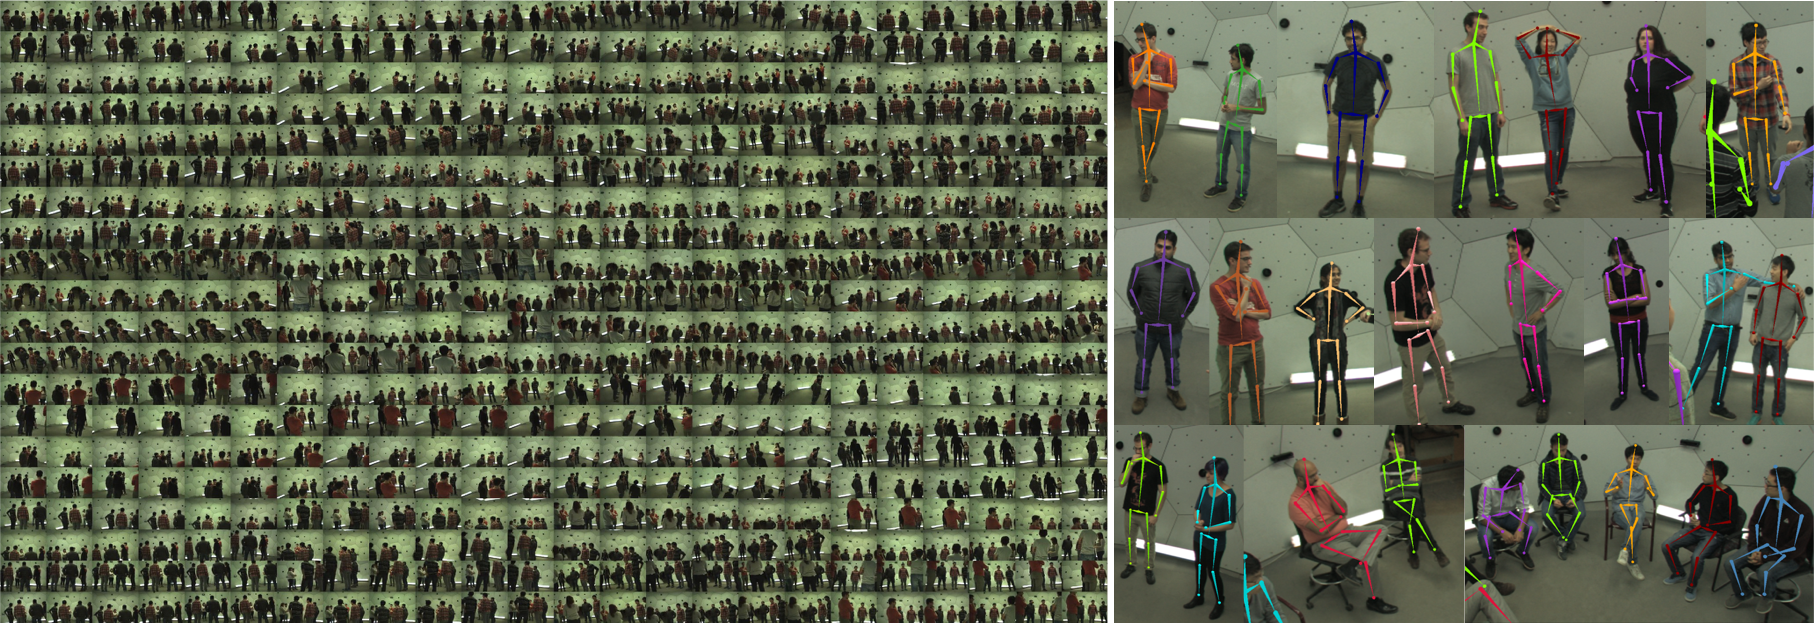
\includegraphics[width=\linewidth]{imgs/Teaser_0814}
%	\caption{(Left) 480 unique VGA views capturing a social interaction within the Panoptic Studio. (Right) HD example views showing frequently occurring postures that carry rich social signals, with 3D body pose automatically annotated by our method.} 
%	\label{fig:iconicPoses}
%\end{figure*}

\chapter{Introduction}
%The way humans communicate is one of the clearest factors that differentiates us from other animals. 
Along with verbal language, we use many other channels for communication, including facial expression, body gestures, hand motions, and interpersonal proximity, collectively referred to as \emph{nonverbal social signals}. The use of all these channels is important in social interactions, where subtle emotions and intentions are transmitted via the combination of such signals~\cite{Moore13}. Endowing machines with such social interaction abilities is an essential goal of Artificial Intelligence (AI) to make machines that can effectively cooperate with humans.% This area is related to multidisciplinary research fields covering psychology, natural language processing, affective computing, human-robot interaction, machine learning, and computer vision.


A way to endow machines with such social skills would be to encode all the rules that humans observe during social communication~\cite{cassell1994animated, cassell2000embodied}. Unfortunately, nonverbal interaction is still poorly understood despite its importance in social communication~\cite{Mehrabian67,Mehrabian81,Birdwhistell-1970}, making it hard to formalize all rules about how to understand and use social signals. An alternative direction of this ``symbolic" paradigm~\cite{newell1976} is to take the ``non-symbolic" (or connectionist) approach~\cite{rumelhart1986parallel} to learn the way humans communicate purely from the data without any hand-coded high level representations. Interestingly, we have recently witnessed significant progress in Natural Language Processing (NLP) showing the potential to allow machines to ``freely'' communicate with humans using written language and speech~\cite{young2018recent}. This success has been led by data-driven approaches leveraging large-scale language datasets and a powerful modeling tool, deep neural networks~\cite{lecun2015deep}, to automatically learn the patterns of human verbal communication. Remarkably, these achievements have not made extensive use of the prior knowledge about grammar and the structure of languages that linguists have accumulated over centuries. Motivated by this, this thesis hypothesizes that a similar approach can be an important breakthrough in modeling nonverbal communication. 

%
%\label{sec:introduction}
%\begin{figure}[h]
%	\centering
%	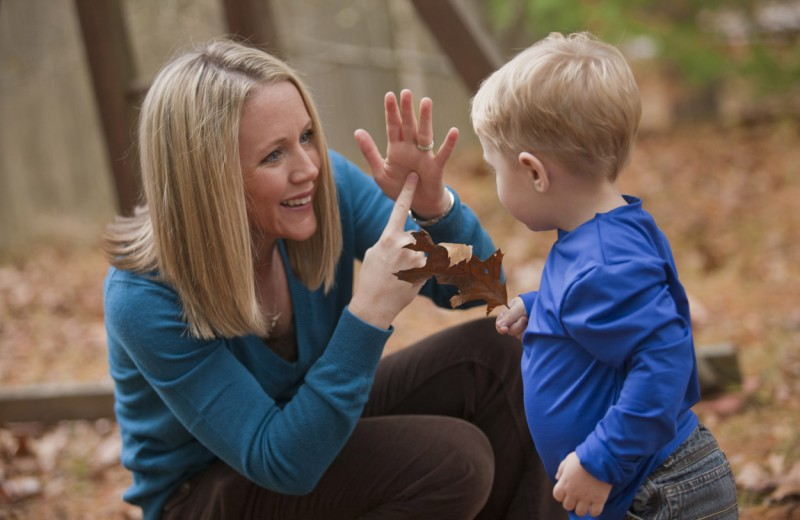
\includegraphics[trim=0 0 0 0, clip=true, height=0.2\columnwidth]{figures/intro_1}
%	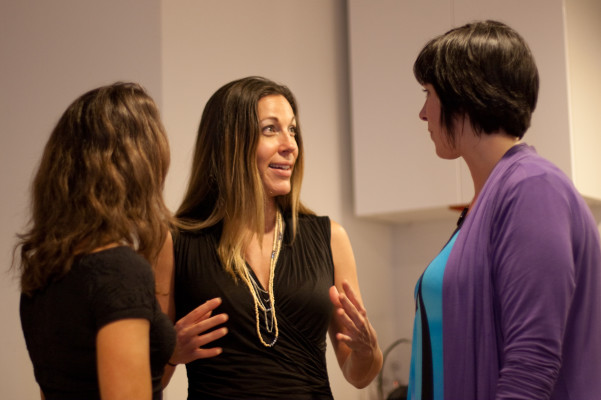
\includegraphics[trim=0 0 0 0, clip=true, height=0.2\columnwidth]{figures/intro_5}
%	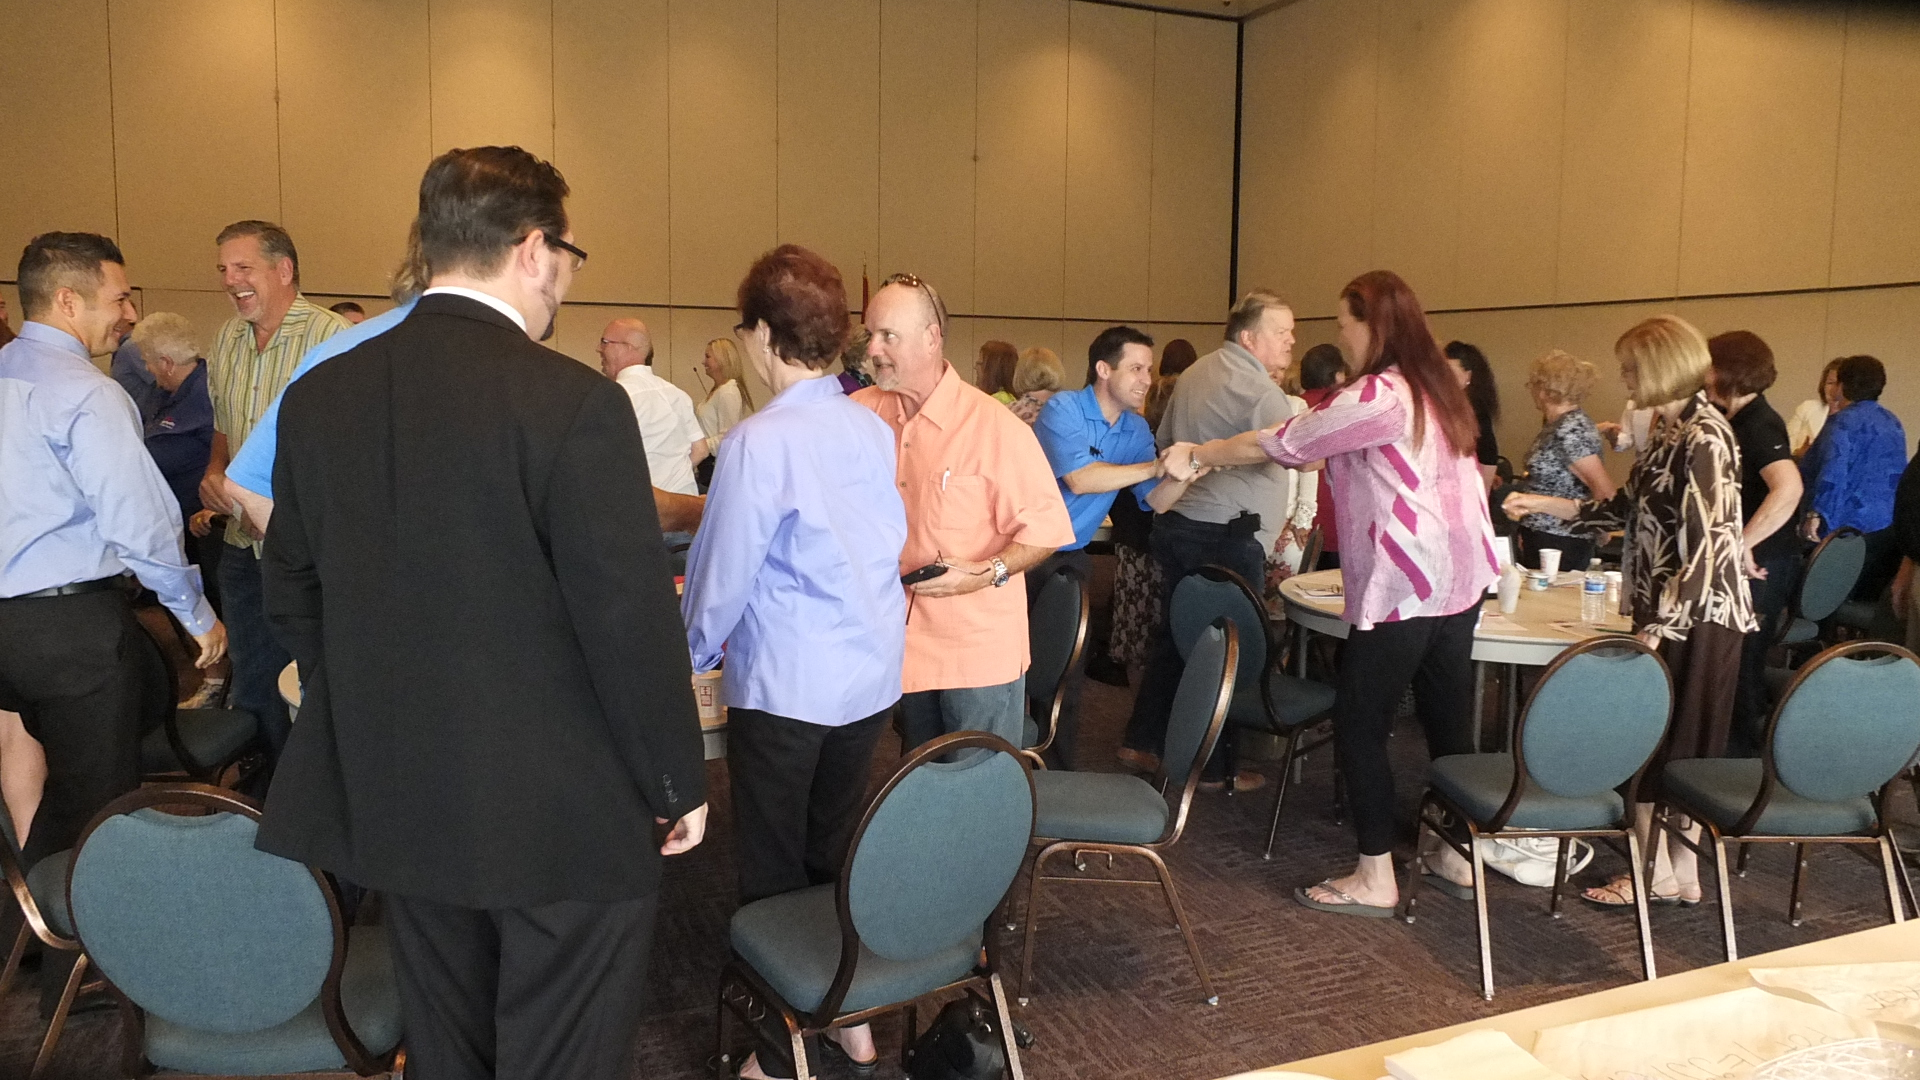
\includegraphics[trim=0 0 0 0, clip=true, height=0.2\columnwidth]{figures/intro_3}
%	\caption{Nonverbal signals play an important role in social communication to transmit messages that cannot be conveyed by verbal language. However, we still lack an understanding of the underlying protocols of these signals. Two major challenges to computationally analyze nonverbal signals in social communication are: (1) measuring the signals at high resolution and (2) modeling nonverbal communication as information flow in the high dimensional space.}	
%	%	\caption{Kinesic signals play important roles in social communication to transmit messages that cannot be conveyed by verbal languages. In this thesis proposal, we present a system and method to measure full body kinesic signals including anatomical landmarks from body, face, and hands. We also propose an approach to model kinesic signals in social interaction by optimizing a prediction function in continuous high bandwidth kinesic signal space.}	
%	\label{fig:ch1_intro}
%\end{figure}


However, there exists a fundamental difficulty in building a data-driven nonverbal communication model: the data is extremely rare. In the verbal language domain, words contain the full expressive power to record verbal signals by a composition of a handful of discrete symbols. Especially on the Internet, there already exist millions of articles or dialogues which are readily usable for data-driven methods (either supervised or unsupervised). However, for nonverbal signals, how to ``record" or collect these signals is uncertain. Imagine a situation where a group of people are communicating in our daily life. The positions and orientations of individuals, their body gestures, gaze, and facial expressions (among others) are the data we are interested in. Notably, these social signals emitted from all people in the group need to be simultaneously sensed to study their correlation and causality. Although there also exist millions of videos where our daily activities---including social interactions---are captured on the Internet, these raw videos cannot be directly used because we have to first measure the behavioral cues (relative location, face, body pose, and so on) from the raw pixels to focus on investigating the rules of nonverbal interactions. %Fortunately, measuring human behavior including person detection~\cite{}, body pose estimation~\cite{}, face keypoint detection, hand keypoint estimation, markerless motion captures have all been greatly advanced, enabling us to collect non-verbal signal dataset.


This thesis explores two scientific questions to computationally study social signals in nonverbal communication: (1) how to measure the ``full spectrum of social signals", including facial expressions, hand gestures, and body motions of an interacting group and (2) how to formalize a ``Connectionist" model by leveraging these new types of signal measurements aiming to teach machines how to decode and encode nonverbal signals to genuinely interact with humans. As major advancements in science are nearly always preceded by innovations in engineering that enable us to measure the world, the first part of this thesis starts by presenting a novel system and method to sense and measure such signals. As a core contribution, a massively multiview capture system, the \emph{Panoptic Studio} shown in the top of Figure~\ref{fig:teaser}, is built to capture naturally interacting multiple people in social situations (Chapter~\ref{chapter:system}). Methods to measure the subtle 3D movements of anatomical landmarks including facial expression, hand gestures, and body motions are also presented, leveraging a large number of views of the Panoptic Studio System (Chapter~\ref{chapter:trajectory}, \ref{chapter:mocap}, and  \ref{chapter:totalcapture}). Our system and method enable us to measure and record the various behavioral cues in face-to-face interactions without using any intrusive devices or artificial markers. 


In the latter part of this thesis, we computationally study the dynamics among interpersonal social signals by leveraging a large-scale social signal corpus built from our system and measurement method. In this research, we verify that the social signals naturally emerging in an interacting group are highly correlated and predictive each other. To achieve the goal, we first collect a large scale dataset where the full spectrum social signals are measured from hundreds of participants in a carefully designed triadic interaction scenario (Chapter~\ref{chapter:dataset}). Then, we formalize a social signal prediction problem as a way to model the dynamics and correlations between various channels of social signals (Chapter~\ref{chapter:prediction}). We explore several social signal prediction tasks defined with various input and output signals to verify the strong links among them. %To this end, we apply the models to build an artificial agent that mimics the nonverbal communication skills of humans, which we refer to as a ``social Artificial Intelligence".

%
%In the latter part of this thesis, we introduce a new research task to build machines that can encode and decode social signals. We hypothesize that the social signals naturally emerging in an interacting group are highly correlated and predictive each other. Thus, we formalize a social signal prediction problem as a way to model such correlation. To demonstrate this, we first collect a large scale dataset where the full spectrum social signals are measured from hundreds of participants in a carefully designed triadic interaction scenario (Chapter~\ref{chapter:dataset}). Then, we leverage this dataset to explore a social signal prediction task to mimic the social behaviors of humans (Chapter~\ref{chapter:prediction}); we formulate that humans are communicating by receiving a set of social signals from others and emitting response signals as output, which are again directed to others as inputs. Machines can learn nonverbal communication skills by automatically finding the patterns between these signal flows. Importantly, our dataset allows us to investigate wide channels of nonverbal cues and their correlations. We explore several subtasks of the social signal prediction to verify the existence of the correlation of social signals, and finally present a framework to build a social Artificial Intelligence by consolidating our social signal prediction modules. 


\section{Key Challenges}
This thesis aims to computationally model social interaction, focusing on nonverbal social signals. Two major challenges in pursuing the direction are addressed.
%To achieve the goal, the signals naturally emerging from interacting people should be obtained first. However, it is challenging to capture and measure such signals in social situations due to multiple challenges addressed in this section. The lack of existing data limits the opportunity to computationally model nonverbal social communication, causing a singular focus on limited measurements and scenarios (e.g., face only~\cite{tronick1989infant} or a table setup allowing limited body motions~\cite{gunes2006bimodal, banziger2012introducing, de2004modeling}). In this thesis, two major challenges in pursuing computational analysis of nonverbal social interactions are addressed.\\ % . 
\paragraph{How To Measure Nonverbal Social Signals:}
To achieve the goal of this thesis, the signals naturally emerging from interacting people should be obtained first. However, it is challenging to sense and measure such social signals, because of the following three reasons. First, during social interactions, strong occlusions emerge functionally (e.g., people systematically face each other while interacting, bodies are occluded by gesticulating limbs). Thus, measurements from a monocular view can hardly capture the entire social signals of all the people involved in the communication (e.g., Figure~\ref{fig:teaser}). Second, subtle motions from faces and hands that play an important role in social interactions should be measured together with large motions from torsos and limbs. This introduces a sensing challenge because often face and hand motions are captured at close range~\cite{beeler2010high,ghosh2011multiview, Beeler2011, bradley2010high, valgaerts2012lightweight, Oikonomidis-12, Tompson-14a, Sridha-15, Tzionas-16}, while torso and limb motions are captured in a sufficiently large working volume where people can freely move~\cite{deAguiar-2008, Gall-09, Stoll-11, Elhayek-15}. Third, the social signals should be measured non-intrusively to allow the people involved a communication to behave naturally and voluntarily. Thus, popular marker-based motion capture systems (e.g., \cite{VICON}) are not applicable. 

Despite the advances in human sensing and markerless motion capture fields in computer vision and graphics, these challenges have not been fully solved yet. Most of the existing methods prior to this thesis focus on the motion of a single subject~\cite{deAguiar-2008,Vlasic-2009,Furukawa2008,Gall-09, Stoll-11, Baak-13,Shotton-13} or exaggerated motions of actors~\cite{Ye-2012,Liu-2013}. Importantly, there is no existing system that can track, without markers, the human body, face, and hands of multiple individuals simultaneously.

Due the limit of available measurement tools, social signals are studied in limited scenarios, for example: (1) studies only focus on face signals ignoring body motions~\cite{messinger2009automated, lucas_trust_2016,mckeown2012semaine}; (2) studies consider situations in a table setup where participants' motions are limited~\cite{carletta2005ami, Lepri-12,messinger2009automated, nojavanasghari2016emoreact, lucas_trust_2016,mckeown2012semaine}; (3) studies assume a small number of people (mostly dyadic communications)~\cite{messinger2009automated,nojavanasghari2016emoreact, lucas_trust_2016, katsimerou2016crowdsourcing,mckeown2012semaine,gunes2006bimodal}.
% 
%
%are rarely measured in social situations, since most of the face and hand systems assume a close distance to the target which can be hardly used for body motion capture system. It is necessary that such signals from faces and hands are measured together with large motion from torsos and limbs, because subtle messages for communications are usually transmitted by the organized motion of the whole body.\\ 
%
%Second, voluntary motions in a social signals should be captured by a non-intrusive method
%
%Third, large motions and subtle details should be capture together. 
%
% This means that a multiview setup to is needed. 
%
% To accurately analyze social interactions, a volume sufficient to house a social group should be assumed, yet all the subtle details of the motion where important social signals are embedded must be captured. A laboratory setup with multiple cameras is preferred to achieve this objective, and it is expected that the sensing challenges can be reduced according to increasing unique view points. However, in most prior work, a few cameras are often used, and, thus, limited research directions are only considered, for example: (1) studies only focus on face signals ignoring body motions~\cite{messinger2009automated, lucas_trust_2016,mckeown2012semaine}; (2) studies consider situations in a table setup where participants' motions are limited~\cite{carletta2005ami, Lepri-12,messinger2009automated, nojavanasghari2016emoreact, lucas_trust_2016,mckeown2012semaine}; (3) studies assume only few number of people (e.g., dyadic communications)~\cite{messinger2009automated,nojavanasghari2016emoreact, lucas_trust_2016, katsimerou2016crowdsourcing,mckeown2012semaine,gunes2006bimodal}.
%
%%\noindent \textbf{How To Measure Kinesic Signals}:  
%For computational analysis, captured raw data (images or videos) should be semantically labeled. For example, a human can infer 3D structure of other people and perceive movements of their anatomical landmarks (e.g., mouth, hands, eyes, and so on). Similarly, it is necessary to measure this semantics of kinesic signals from captured images and videos to make machines to decode their meaning. Importantly, these kinesic signals should be measured non-intrusively to avoid potential primes in natural interactions, and, thus, artificial markers or a specialized suit often used in motion capture system should not be exploited. Markerless motion capture in computer vision tackles this challenge, but most previous work is demonstrated in the scenes that are far from social situations, often capturing a single subject only, and assuming a predefined 3D template for each individual~\cite{Gall-09, Vlasic-08, Brox-10, Stoll-11, deAguiar-2008, Vlasic-2008}. Motions from faces and hands that play an important role in social interactions are rarely measured in social situations, since most of the face and hand systems assume a close distance to the target which can be hardly used for body motion capture system. It is necessary that such signals from faces and hands are measured together with large motion from torsos and limbs, because subtle messages for communications are usually transmitted by the organized motion of the whole body.\\ 
%\mbox{ }\\
\paragraph{How To Model Nonverbal Communications:} 
Modeling social signals using computational methods is a largely unexplored area due to the following four reasons. First, the lack of available dataset or measurement technology limits the opportunity to computationally investigate the social signal modeling. Because of this reason, studies on body gestures are relatively rare~\cite{gunes2006bimodal, banziger2012introducing, de2004modeling}, while many researchers focus on facial expressions exploiting existing automatic measurement tools~\cite{Torre15} with an existing coding system~\cite{ekman1977facial}. Similarly, although we want to investigate the correlation between various behavioral cues (e.g., facial expression and hand gestures), the challenges in simultaneously measuring these signals make it hard to explore this direction.

Second, there is no good way to represent and objectively annotate the semantics embedded in social signals. For example, a ``smile" signal, formed by flexing the muscles at the side of the mouth with a contraction of the muscles at the corner of the eyes, may be recognized as ``happiness". However, the internal emotion expressed by the signals may not be simply annotated by a discrete status of ``smile" or ``happiness", because it may have a variety of subtly different meanings depending on the intensity of the facial movements. Importantly, the mapping between the social signal measurements to the semantic space is subjective to the observers~~\cite{steidl2005all}.

Third, the high complexity of social signals that are located in a continuous and high dimensional space makes the modeling harder. Unlike words, the start and end timing of social signals are ambiguous. The organized motions from torso, face, and hands need to be considered together~\cite{aviezer2008angry,barrett2011context}. A social interaction among multiple people (more than two) is also challenging due to the diversity of interactions. All these challenges make computational social signal modeling difficult.

Finally, it is unclear how to evaluate the performance of the model. For example, a social signal prediction model may generate a ``realistic" nonverbal signals, but we are lack of methods to quantify how realistic the output is.

%Modeling social signals using computational methods is a largely unexplored area due to the limited availability of the data. Most of the previous work focuses on recognizing coarse semantics from the signal measurements\cite{ekman1969, osgood1952nature, russell1979affective, plutchik2001nature}. For example, a smile signal, formed by flexing the muscles at the side of the mouth with a contraction of the muscles at the corner of the eyes, may be recognized as happiness. However, the internal emotion expressed by the measured signals cannot be simply annotated by the words of ``smile" or ``happiness", because it may have a variety of subtly different meanings and intensities depending on the spatial and temporal variations of the facial movements. These approaches are fundamentally limited, because: (1) the semantic dimensions or categories are hand-designed without a clear evidence that it fully covers the entire internal status of humans and (2) the mapping between the social signal measurements to the semantic space is subjective to the observers. Furthermore, most of these approaches focus on facial expressions, and study for body gestures are rarely investigated~\cite{gunes2006bimodal, banziger2012introducing, de2004modeling}. How to teach machines to use social signals (encoding the social signals) in responding to conversational partners during social interactions is also poorly explored.

%Most prior approaches focus on deciphering the semantic meanings of social signals, which are often annotated into a few discrete categories~\cite{ekman1969} or a set of latent dimensions\cite{osgood1952nature, russell1979affective, plutchik2001nature} (see a recent survey~\cite{noroozi2018survey}). These approaches, however, are fundamentally limited, because: (1) the semantic dimensions or categories are hand-designed without a clear evidence that it fully covers the entire internal status of humans and (2) the mapping between the social signal measurements to the semantic space is subjective to the observers. Especially, these approach may be able to make machines to recognize coarse semantic meanings of humans behaviors (decoding the social signals), but cannot teach how to use such signals (encoding the social signals) in responding to conversational partners during social interactions. %Especially, recognizing a combination of all body movements as a single semantic label (either a category or a point in the latent dimensions) is extremely ambiguous. 
 
 %The Figure~\ref{fig:kinesicflow} describes an information flow in kinesic communication between individuals, where an encoding and a decoding between signals and messages are continuously performed. These approaches, however, are fundamentally limited, because we cannot objectively measure or represent the internal status (e.g., the messages conveyed by signals and their interpretations in Figure~\ref{fig:kinesicflow}), but only can measure the exposed signals themselves.

%Prior work annotate social signals (e.g., face landmarks and EMG sensor output) by a few manually defined categories in quantized degrees (e.g., sentiment), but it basically assumes a mapping from the high dimensional continuous signals to a low dimensional discrete space, losing large amount of subtle details of signals.\\

%	\begin{figure}[t]
%		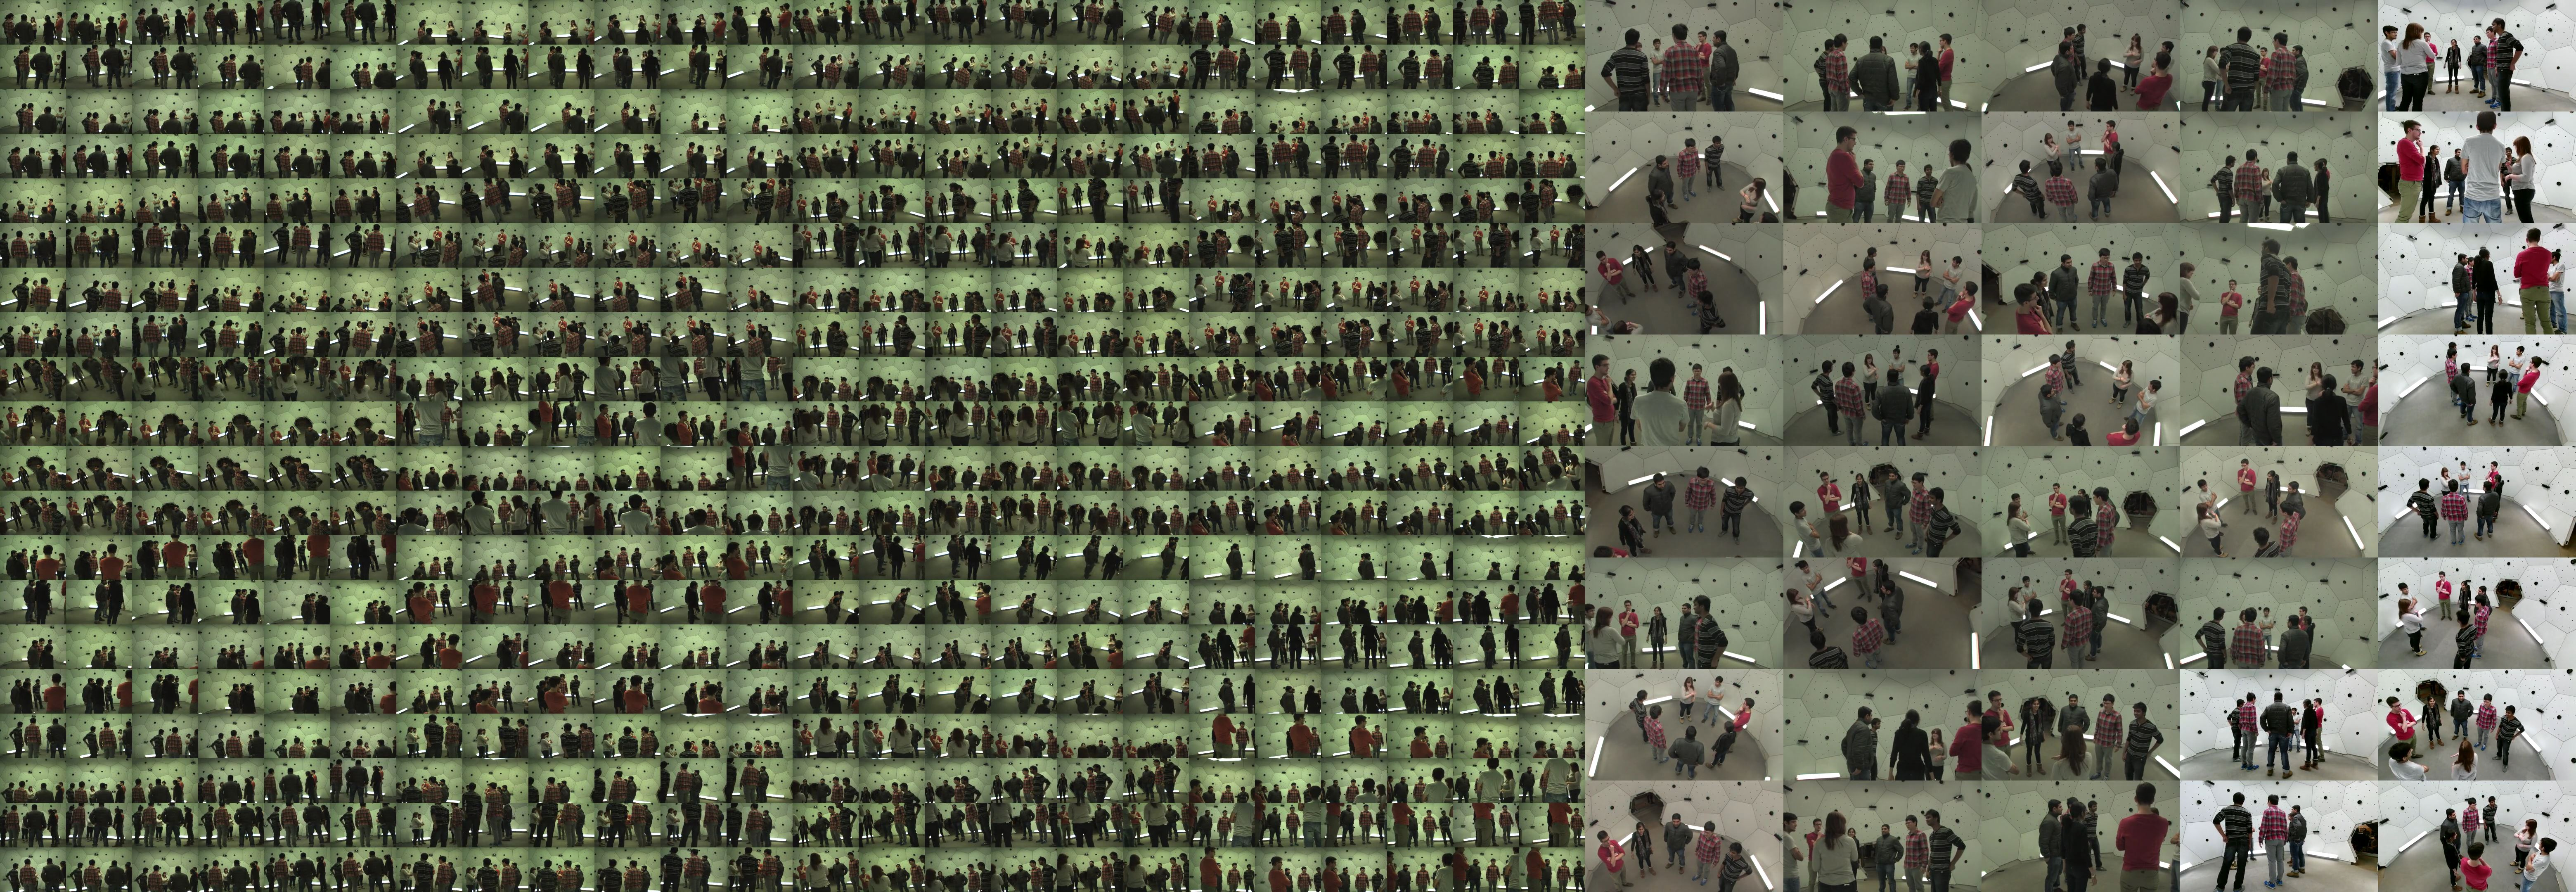
\includegraphics[width=\linewidth]{figures/Teaser}
%		\caption{521 unique views by 480 VGAs, 31 HDs, and 10 RGB+D sensors capturing a social interaction within the Panoptic Studio.} 
%		\label{fig:panopticviews}
%	\end{figure}

%
%\begin{figure}[t]
%	\centering
%	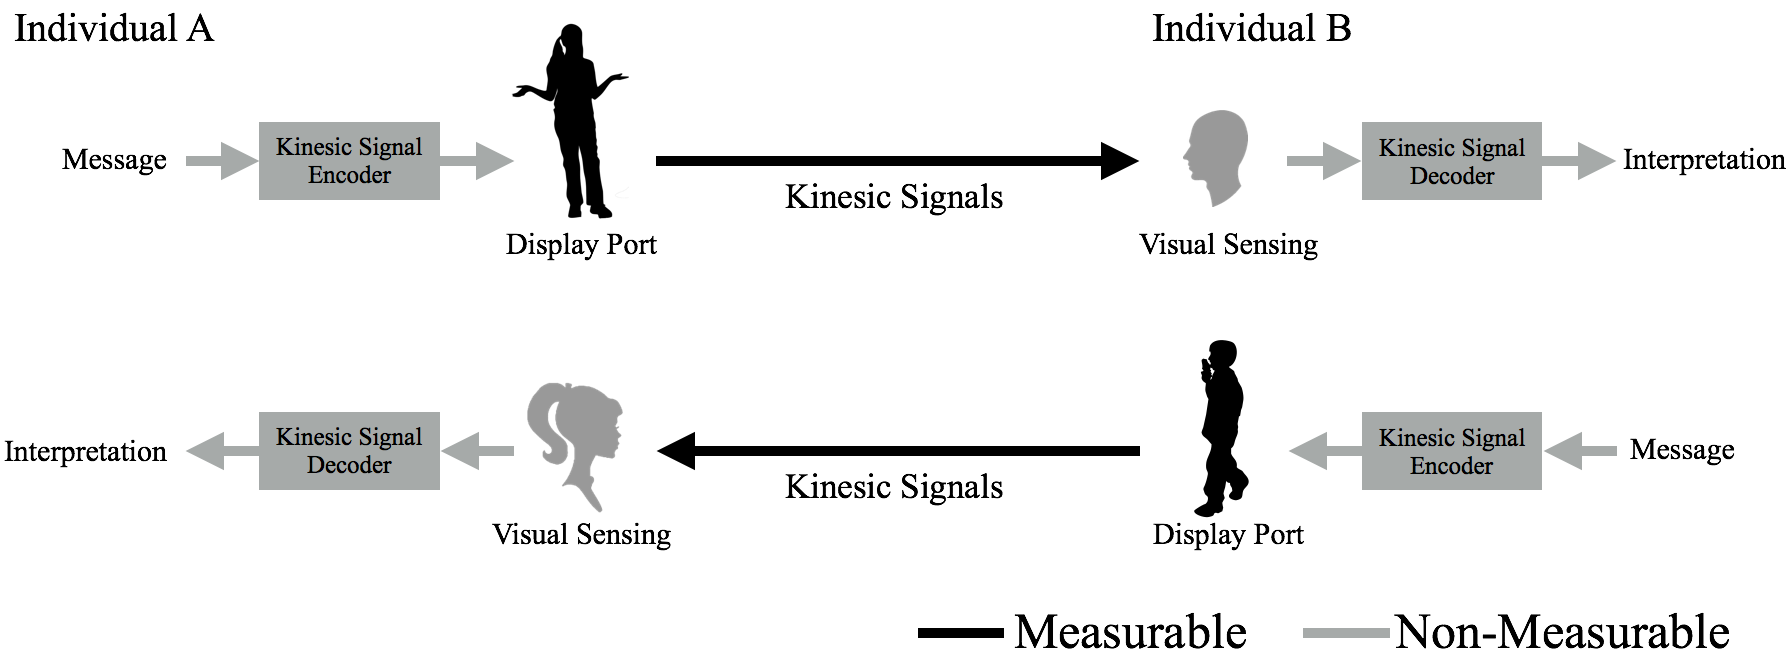
\includegraphics[trim=0 0 0 0, clip=true, width=\textwidth]{figures/kinesicflow2}
%	\caption{Kinesic communication can be considered as an information flow among people. Messages are converted by an encoder and transmitted by our body as a form of kinesic signals. The transmitted signals are sensed, decoded, and finally interpreted by a receiver. We have no clear way to measure the flow or status inside our mind, but only can measure the exposed signals.}	
%	\label{fig:kinesicflow}
%\end{figure}


\begin{figure}[t]
	\centering
	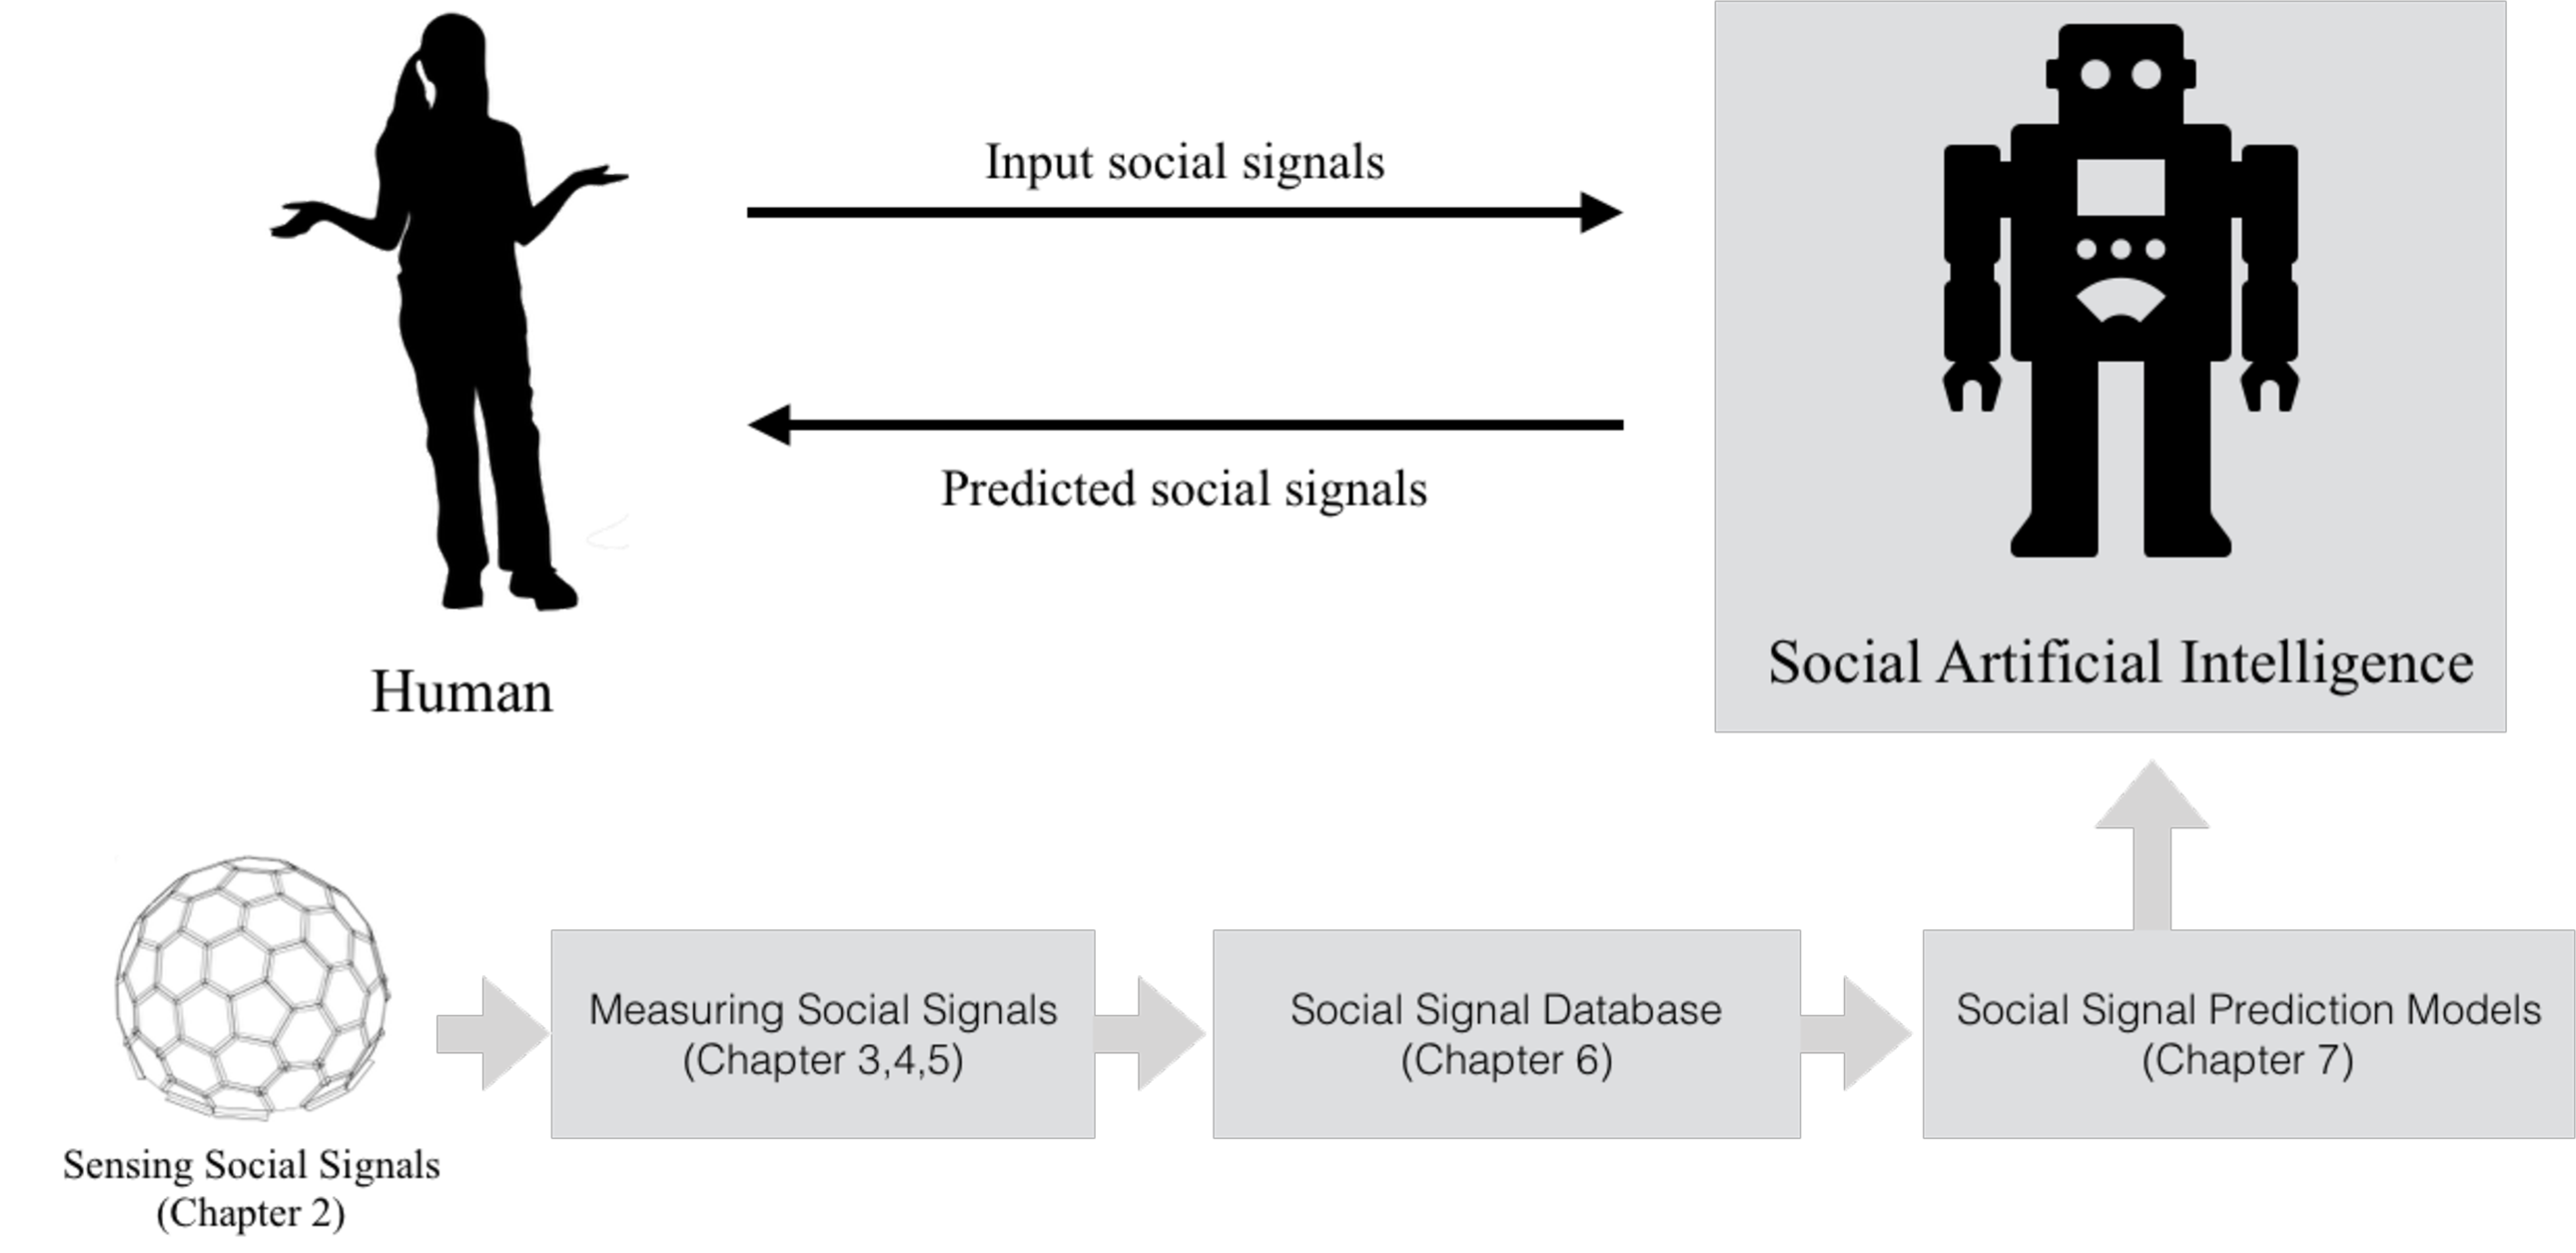
\includegraphics[trim=0 0 0 0, clip=true, width=\textwidth]{figures/intro_framework}
	\caption{Thesis overview. We explore new approaches in sensing, measuring, and modeling social signals to ultimately endow machines with nonverbal communication abilities}	
	\label{fig:thesis_overview}
\end{figure}



\section{Thesis Contribution}

\noindent \textbf{Thesis statement.}
\emph{We advocate that the full spectrum of social signals---including the body gestures, facial expression, and hand motion---of a naturally interacting group can be measured by a system with a sufficient number of cameras. Based on the measurement, we also argue that such naturally emerging social signals are predictive each other, and modeling their correlation is crucial to enable social Artificial Intelligence.}\\
\mbox{ }\\
\indent This thesis presents a ``full-stack" framework to apply computational methods to model nonverbal social communication. The core contribution of thesis spans a new sensor system to capture interacting multiple people (Chapter~\ref{chapter:system}), a novel methodology to measure the full spectrum of social signals (Chapter~\ref{chapter:trajectory}, \ref{chapter:mocap}, and  \ref{chapter:totalcapture}), a large-scale social interaction dataset (Chapter~\ref{chapter:dataset}), and formalizing a predictive model of social signals (Chapter~\ref{chapter:prediction}). The core contributions of this thesis are summarized below and an overview of this thesis is illustrated in Figure~\ref{fig:thesis_overview}.
%
%creation of a new scientific discipline of computational behavioral science,
%by measuring the full spectrum of social signals transmitted during interpersonal social interaction.
%
%
%
%The objective of this thesis is to develop a system to measure and model kinesic signals of interacting people. As a core contribution, we build a massively multiview system, the CMU Panoptic Studio, which is composed of 521 heterogeneous camera sensors. Based on the system, we present a method to measure the full spectrum of 3D kinesic signals of interacting multiple people, including the subtle motions of faces, hands, feet, and bodies. Example results are shown in the Figure~\ref{fig:teaser}. A large-scale dataset capturing the interactions of a large number of groups are collected and publicly released\footnote{Panoptic Studio Dataset: \url{http://domedb.perception.cs.cmu.edu/}}.
%
%We also present a framework to model kinesic signals as an information flow among people, by presenting a method to predict kinesic signals of an individual in a social situation. The goal is to build a model to mimic the social communication of humans by producing appropriate response kinesic signals by receiving other people's kinesic signals as input. The model is trained using a Deep Neural Network with a large scale interaction dataset we have collected. We also leverage our social signal prediction model to quantify the amount of information emitted by each body part, which can be interpreted as a way to measure how each channel of kinesic signals contributes in kinesic communication. 

\subsection{Panoptic Studio: A Massively Multiview System (Chapter~\ref{chapter:system})}
We built a new sensor system, the Panoptic Studio, specifically designed to overcome the sensing challenges emerging in social situations. The system is composed of 521 synchronized sensors with different types, including 480 VGA cameras, 31 HD cameras, and 10 RGB+D sensors. The large number of sensors densely cover a large capture volume (5.49$m$ of a diameter) sufficient to have multiple people, enabling to relieve occlusions among interacting people. 

We present a novel modularized design architecture to simplify the complexity of the system. The system is composed of repeated modules with the same shape and architecture, and each module is controlled by a separate local machine. This modularized design makes it easy to control and manage the system, and also enables efficient data acquisition by saving data locally. All cameras are accurately synchronized (or temporally aligned) by a hardware clock, and spatially calibrated in a common 3D world space. The core design choices and technical solutions including structural design, architecture, temporal calibration, and spatial calibration are addressed in Chapter~\ref{chapter:system}.

%, and densely cover the capture volume (5.49$m$ of a diameter) sufficient to have multiple people. The system is composed of three type of sensors: 480 VGA cameras, 31 HD cameras, and 10 RGB+D sensors. The VGA cameras are chosen to have more viewpoints given the same pixel budget, while HD cameras are necessary to capture the detailed structure of body parts such as faces and hands. RGB+D cameras make it easier to obtain a dense 3d point cloud at each time regardless the colors and textures of people. The combination of sensors contribute together in measuring kinesic signals at high resolution including the motion of 3D anatomical landmarks of full body, face, and hands, as well as measuring a dense 3D surface movement. 


\subsection{Measuring 3D Social Signals (Chapters~\ref{chapter:trajectory},~\ref{chapter:mocap},~\ref{chapter:totalcapture})}

We present the first method to measure the full spectrum of 3D social signals including subtle motions from body, face, and hands. The core goals in developing the methods are: (1) simultaneously capturing the \emph{total body motion} of all body parts when a group of people are naturally interacting; (2) building a fully automatic method to capture social sequences at scale without human labor; (3) minimizing assumptions about scenes to be applicable in any type of motion and appearance of arbitrary number of people; and (4) avoiding intrusive approaches, such as attaching artificial markers and avoiding a tedious 3D template building step. To this end, we present a method based on ``weak'' perceptual processes from a large number of views, and robustly measure social signals by satisfying the aforementioned principles. In Chapter~\ref{chapter:trajectory}, a method to reconstruct dense surface movements, which we refer to as a ``trajectory stream", is presented by fusing optical flow cues from the large number of views in 3D. The core challenge of the method is to reason about a time varying visibility to fully exploiting the large number of views. In Chapter~\ref{chapter:mocap}, reconstructing the movement of 3D anatomical landmarks is presented. In this method, we run 2D keypoint detectors for body, face, and hands respectively in each view, and fuse them in 3D to reconstruct 3D locations of anatomical landmarks. By associating them with the trajectory stream, we obtain accurate markerless motion capture results, as well as semantic labeling of the trajectory stream.  In Chapter~\ref{chapter:totalcapture}, we present a novel 3D deformable human body model for total body motion capture, which can express the motions from full body including facial expression and hand gestures in a unified parametric space. 


	
%\noindent \textbf{Proposed Work:} The current measurement results will be spatially and temporally improved by using temporal cues and dense point clouds from multiple RGB-D cameras. Our current method are presented for the goal in this thesis proposal, but it is not able to be applied to long-term sequences of our dataset due to the heavy computational cost. 

%\begin{figure}[t]
%	\centering
%	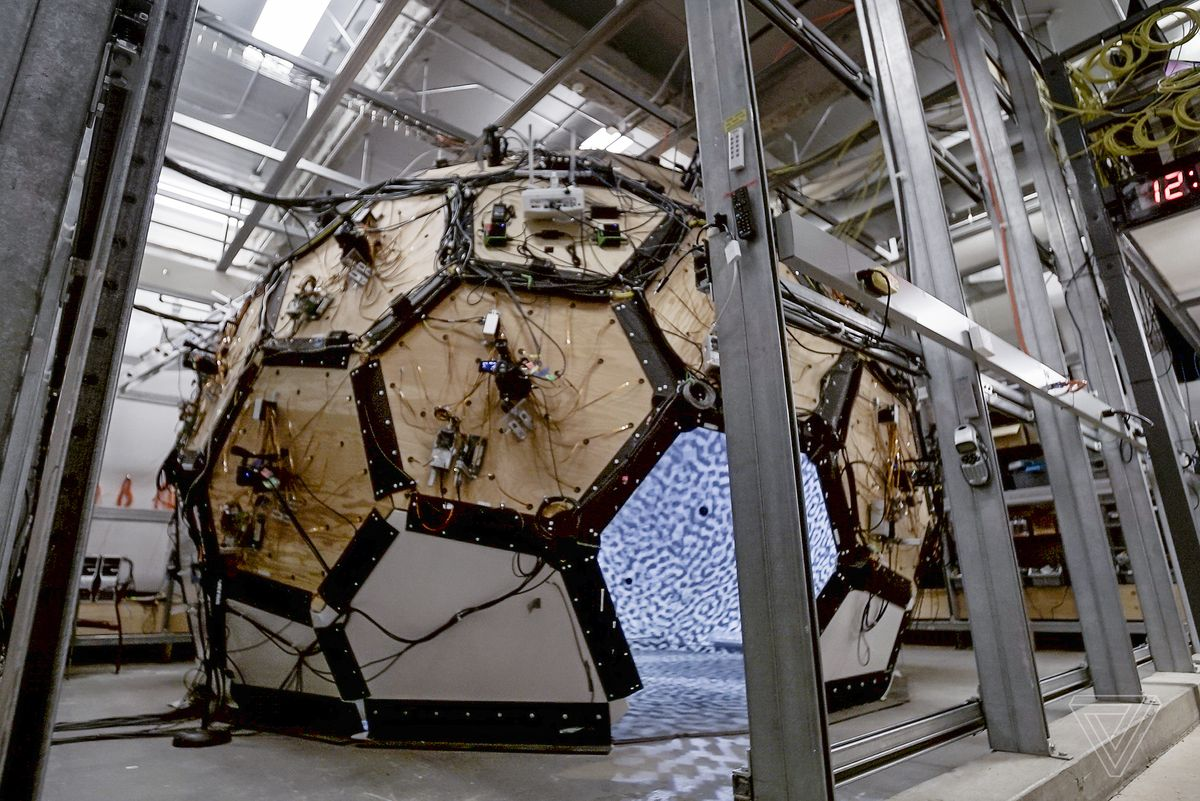
\includegraphics[trim=0 0 0 0, clip=true, width=0.32\textwidth]{figures/panoptic}
%	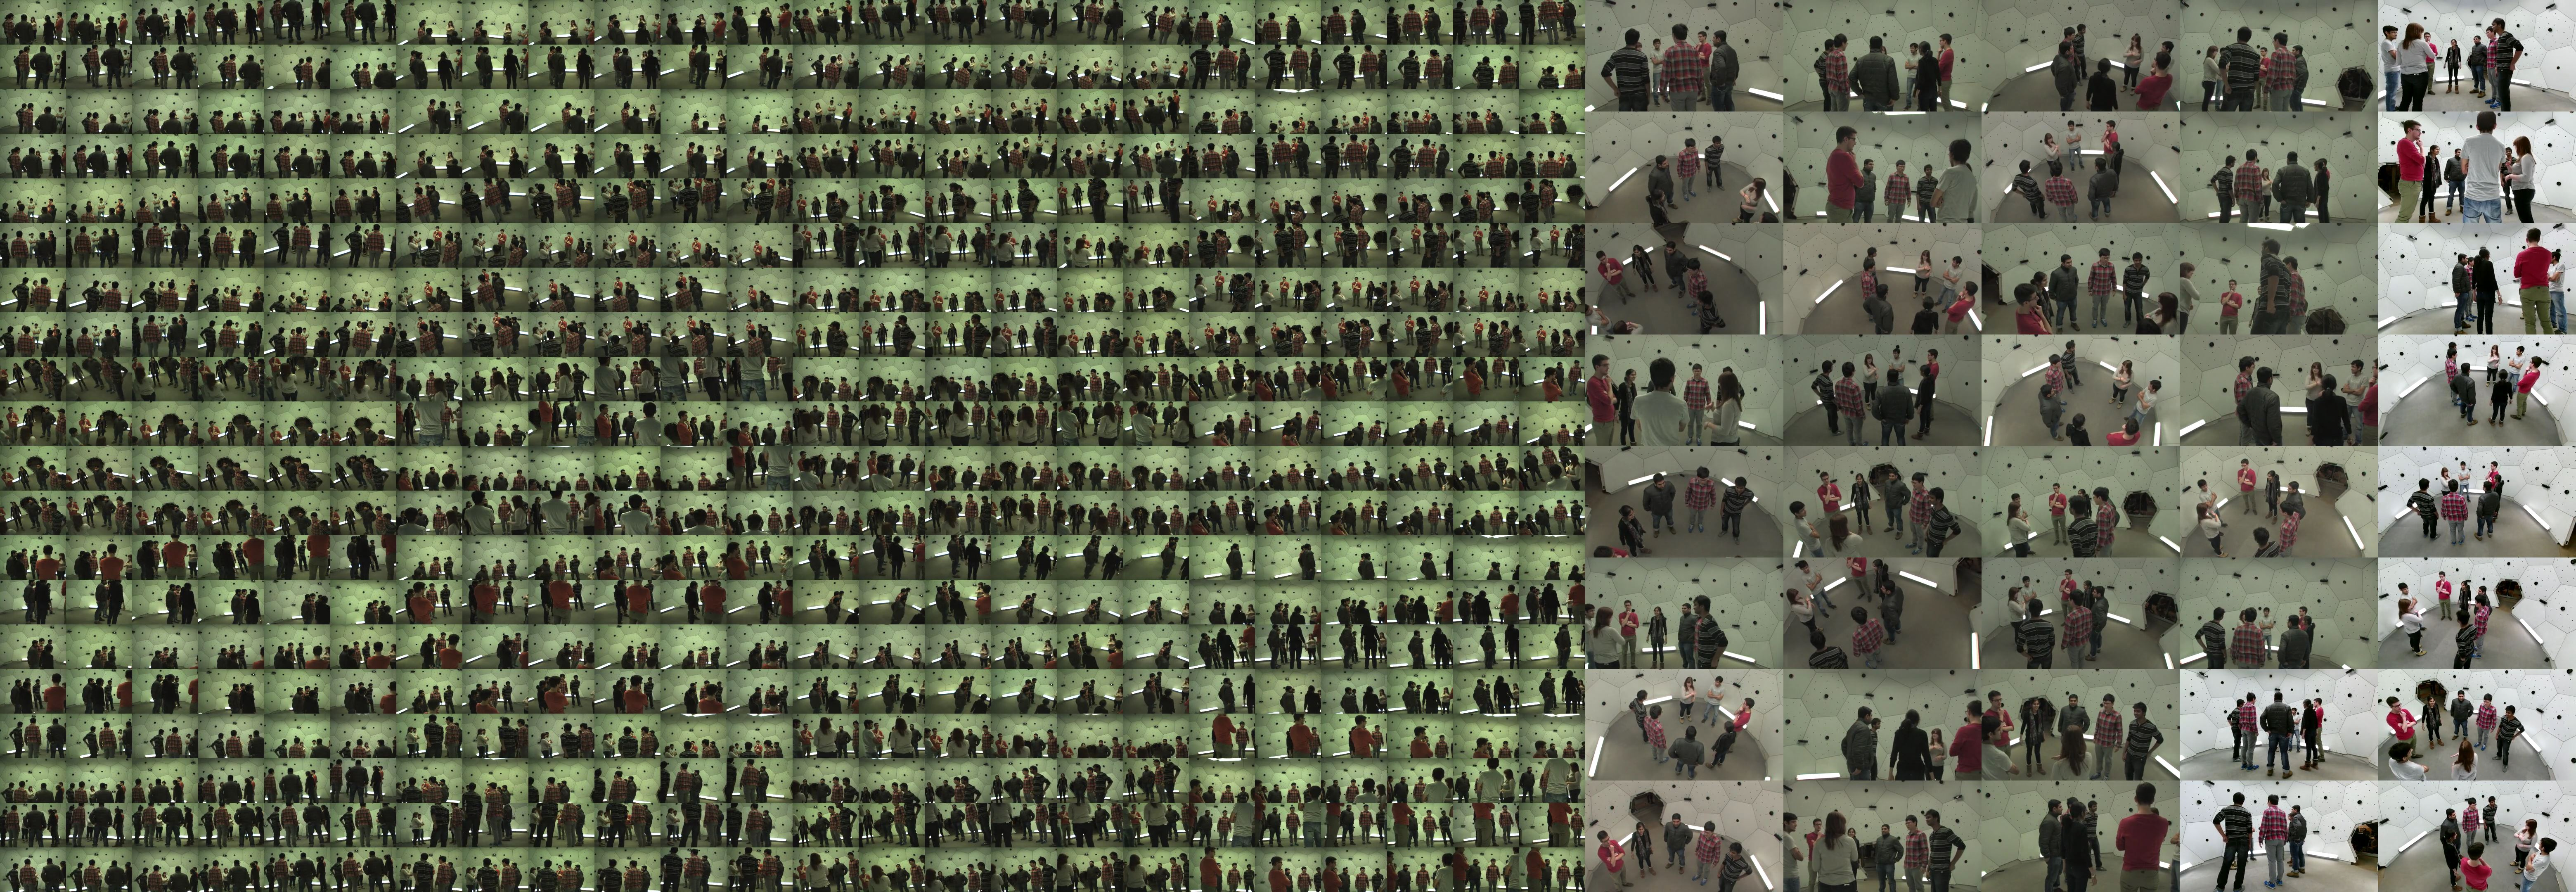
\includegraphics[width=0.62\textwidth]{figures/Teaser}\\
%	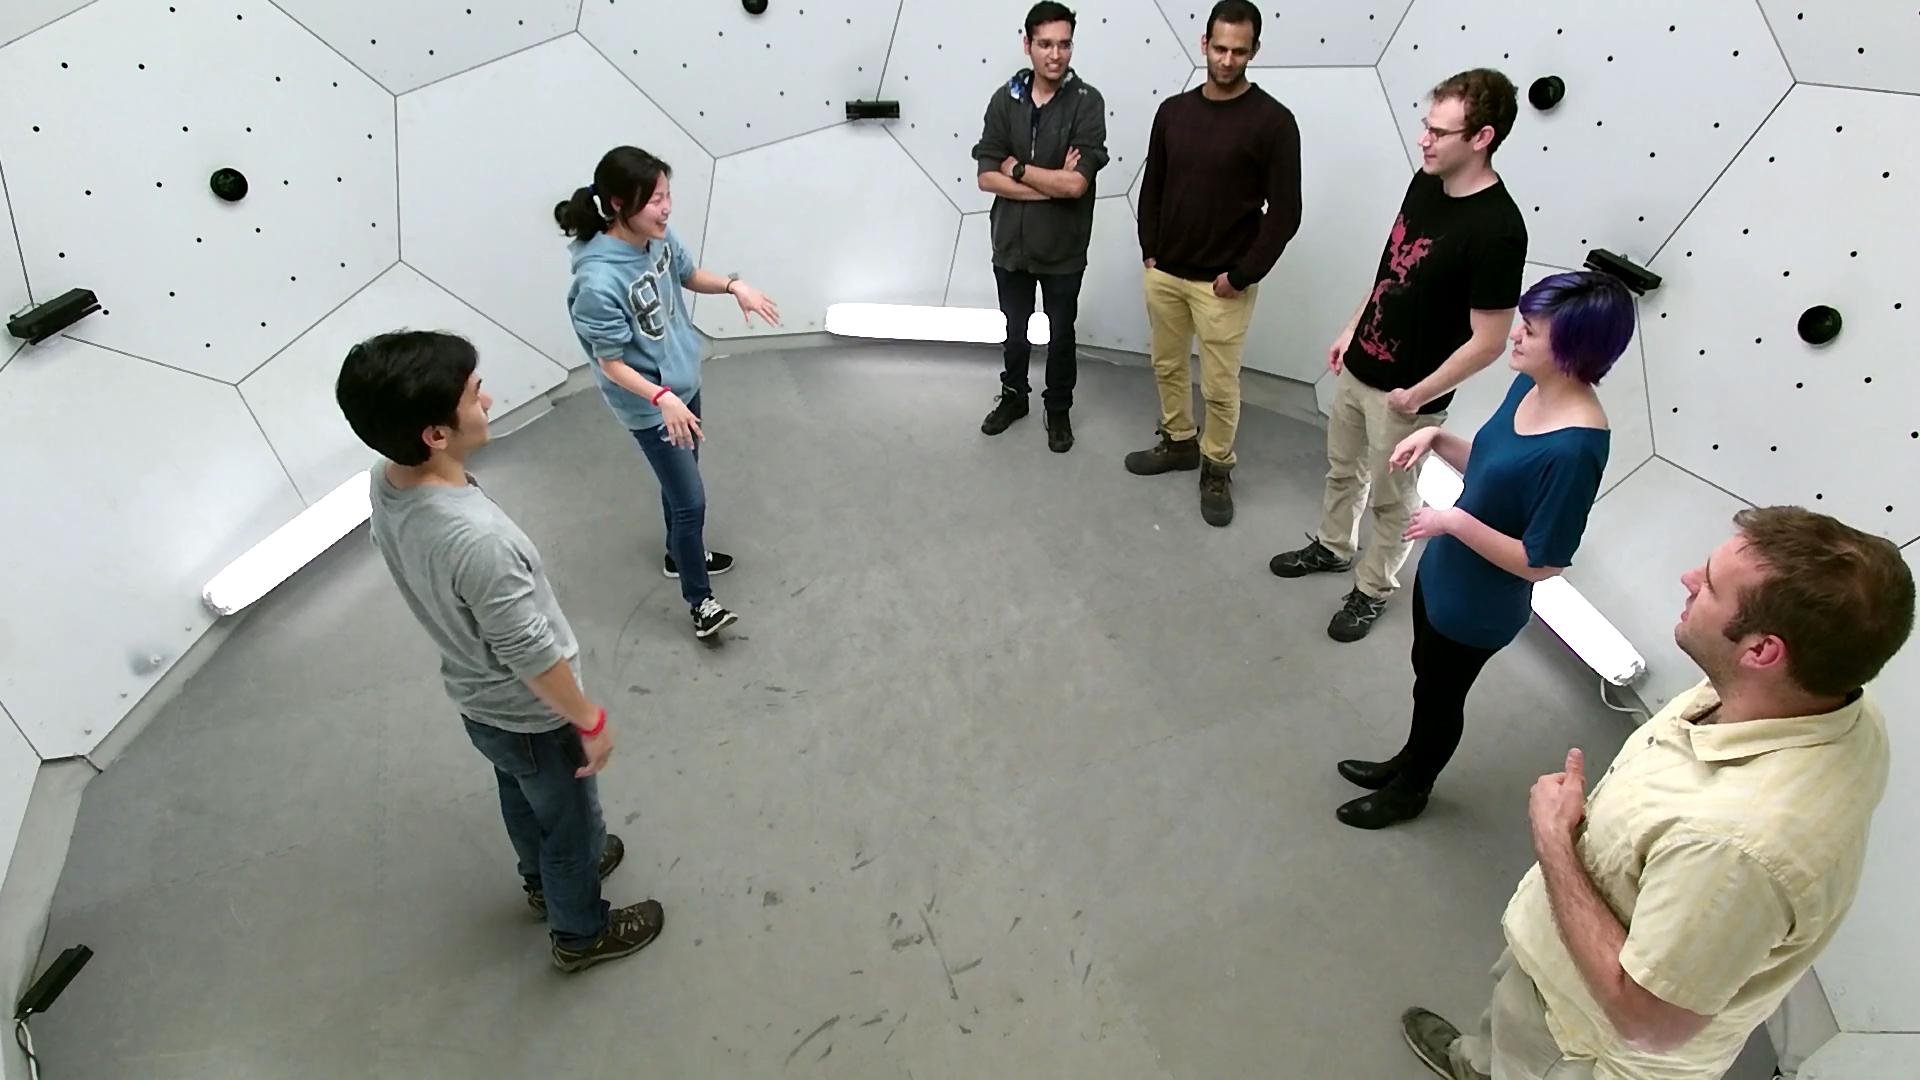
\includegraphics[trim=0 0 0 0, clip=true, width=0.311\textwidth]{figures/teaser_1}
%	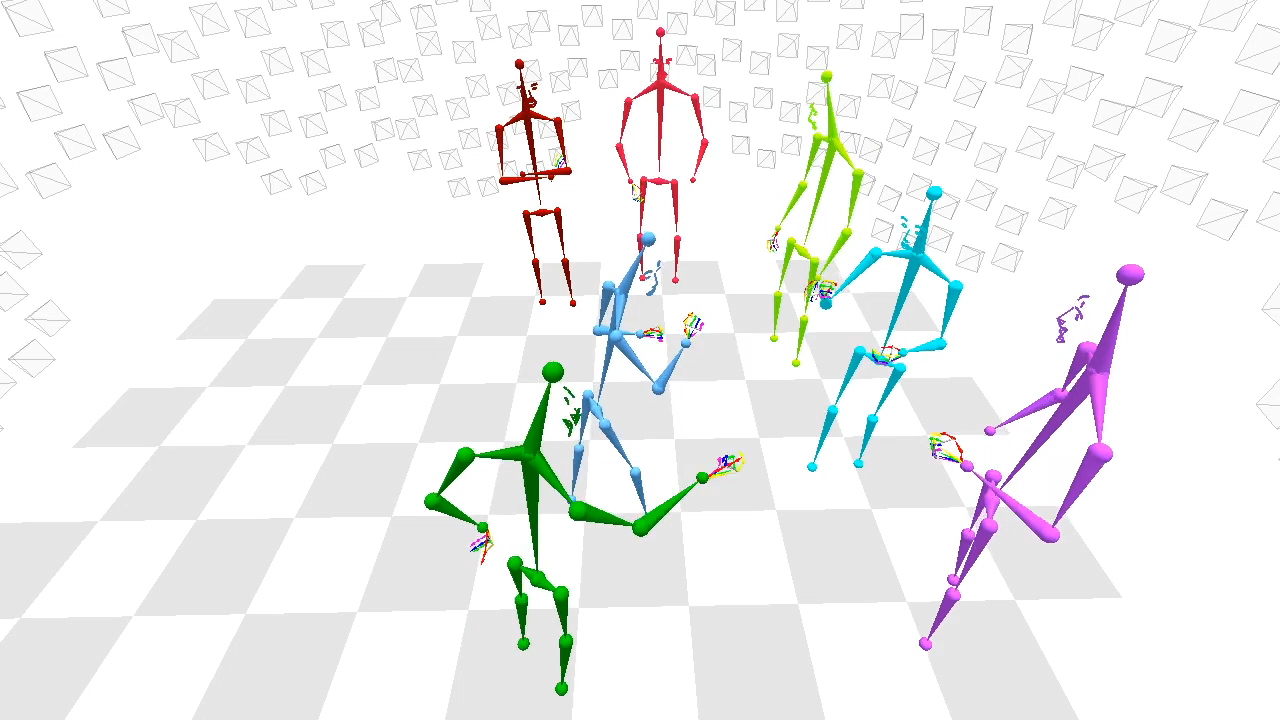
\includegraphics[trim=0 0 0 0, clip=true, width=0.311\textwidth]{figures/teaser_2}
%	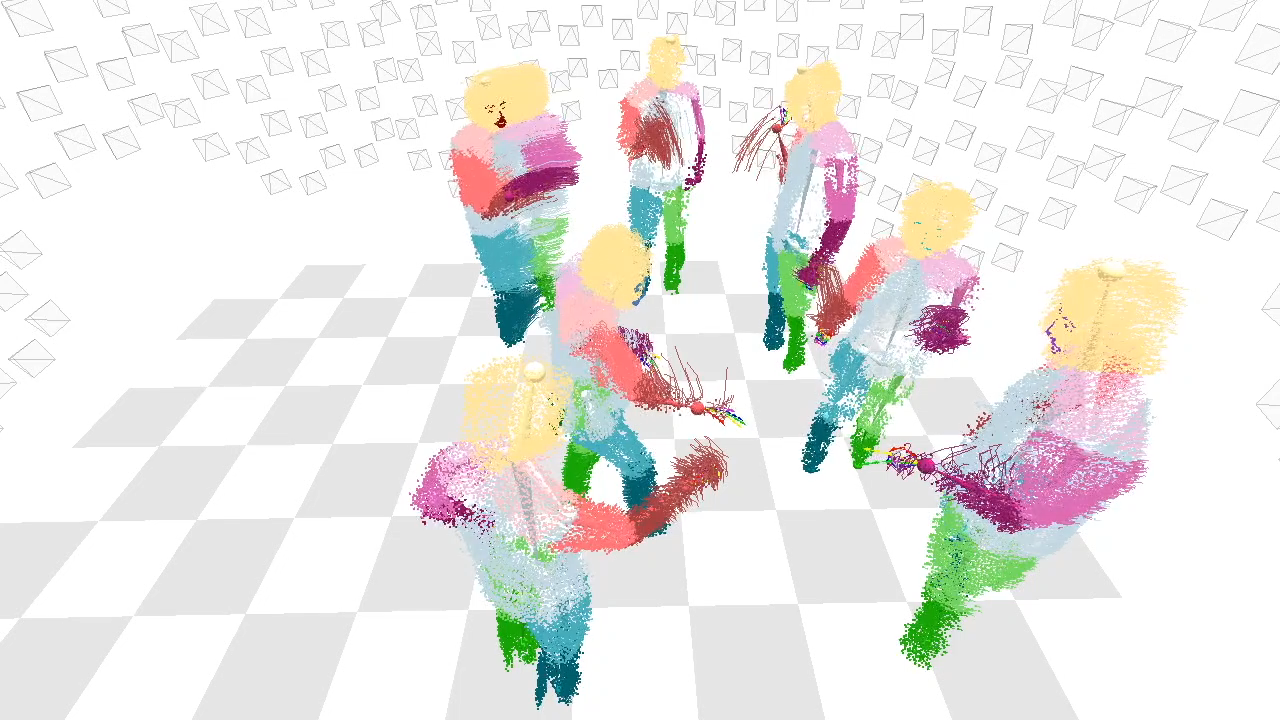
\includegraphics[trim=0 0 0 0, clip=true, width=0.311\textwidth]{figures/teaser_3}
%	\caption{(Top left) The Panoptic Studio, (Top right) 521 unique views by 480 VGAs, 31 HDs, and 10 RGB+D sensors capturing a social interaction within the Panoptic Studio, (Bottom) An example scene captured in the Panoptic Studio and measured kinesic signals.}	
%	\label{fig:teaser}
%\end{figure}


\begin{figure}[t]
	\centering
	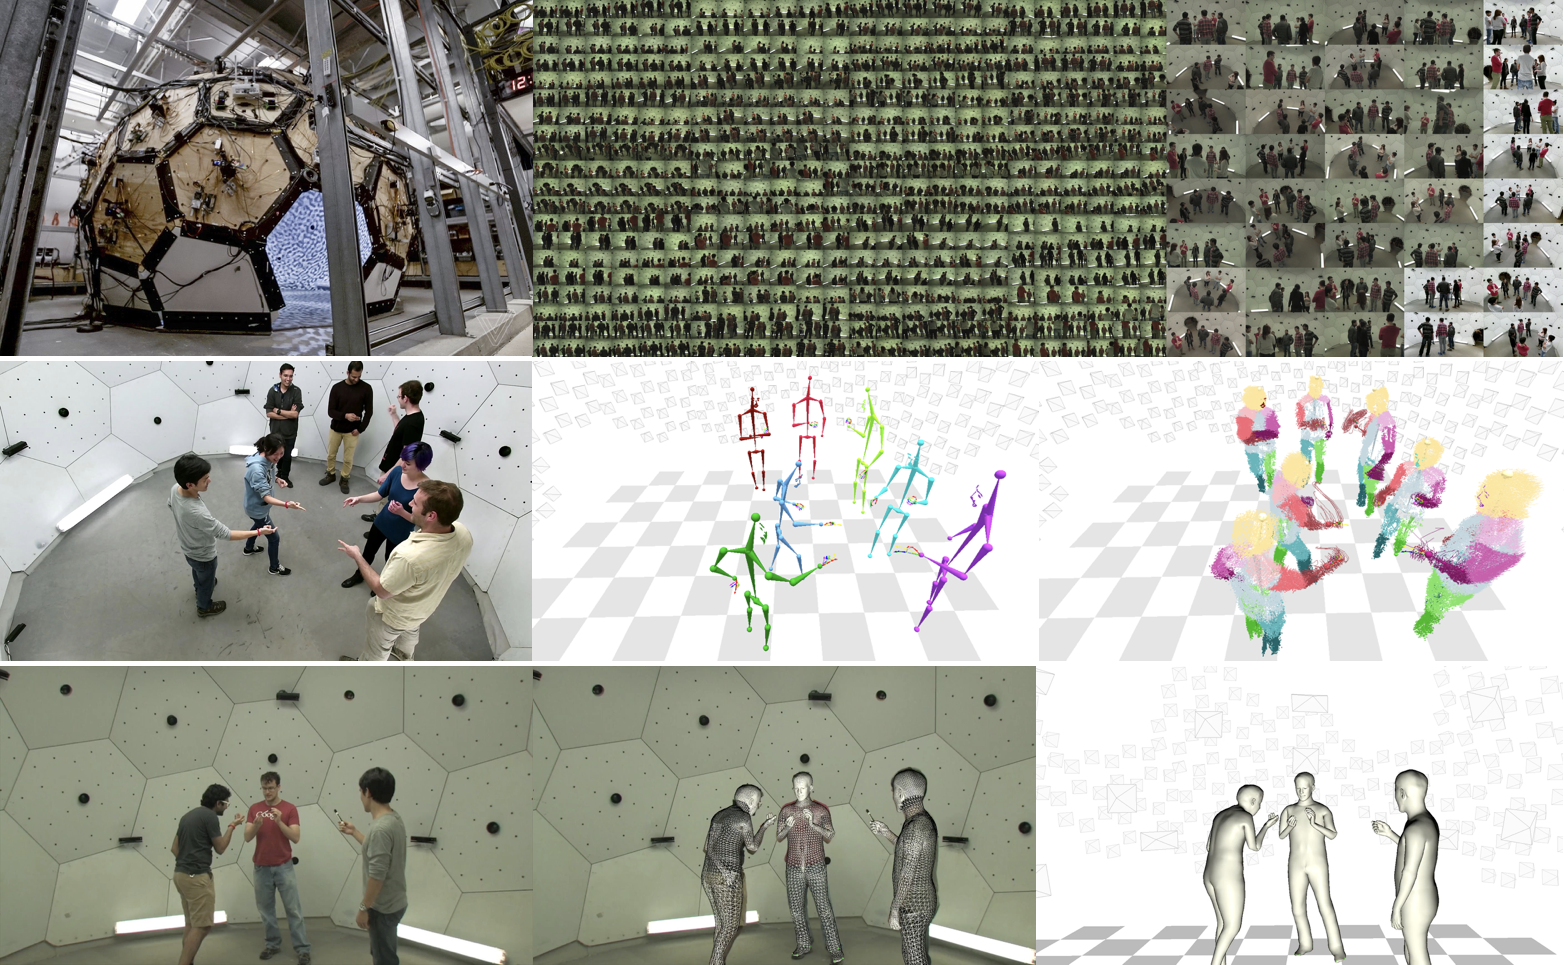
\includegraphics[width=\textwidth]{figures/teaser_4}
	\caption{(Top left) The Panoptic Studio; (Top right) 521 unique views by 480 VGAs, 31 HDs, and 10 RGB+D sensors capturing a social interaction within the Panoptic Studio; (Middle left) An example scene captured in the Panoptic Studio; (Middle center) Measured anatomical landmarks from bodies, faces, and hands; and (Middle right) Measured motion of dense 3D surface points of multiple people; (Bottom) a total motion capture result by the Adam model, showing an input image (left), the reconstruct mesh models overlaid on an input image (middle), and a 3D view (right).}	
	\label{fig:teaser}
\end{figure}

\subsection{A Large-Scale Human Motion Database (Chapter~\ref{chapter:dataset})  }
We build a large-scale dataset by capturing face-to-face interactions of hundreds of participants in our Panoptic Studio. The scenes are captured in a carefully designed triadic negotiation scenario, referred to as \emph{Haggling}, where voluntary social behaviors can naturally emerge. The common social scenario makes it easier to model social interaction, by putting all the subjects in the same social situation. The various behavioral cues including facial expressions, body motions, hand gestures, and individual voices, are sensed and measured by our markerless motion capture system. 

Along with the social game dataset, we also use our system to capture other motions to build a large-scale 3D human motion database. Our database contributes to invent new computer vision techniques. For example, our dataset enables us to build a popular hand keypoint detector~\cite{simon2017hand} in the OpenPose Library~\cite{openpose}, the first deformable 3D human model for total motion capture~\cite{joo2018}, and the first monocular 3D human total capture method applicable in-the-wild~\cite{Xiang2019}. Importantly, we publicly released our dataset in our database website\footnote{\url{http://domedb.perception.cs.cmu.edu}}.

\subsection{Formalizing Social Signal Prediction To Model Nonverbal Interactions  (Chapter~\ref{chapter:prediction})}

We introduce a \emph{Social Signal Prediction} task as a way to computationally model nonverbal interactions. The objective of this task is to predict the behavior of a target person in a social situation. We hypothesize and verify that a target person's behavior is correlated to the behavioral cues of other individuals. For example, the location and orientation of the target person should be strongly affected by the position of conversational partners (known as Proxemics~\cite{Hall66} and F-formation~\cite{kendon90}), and the gaze direction, body gestures, and facial expressions of the target person should also be ``conditioned" by the behaviors of the conversational partners. In this social signal prediction task, we model this conditional distribution among interacting subjects, to ultimately teach a robot how to behave in a similar social situation. In Chapter~\ref{chapter:prediction}, we present several subtasks in modeling a subset of social signals among subject involved in a social interaction, and demonstrate their social signals are predictive. To this end, we present a framework to mimic the nonverbal behavior of the target person responding to other subjects' behavior.%, which we call social Artificial Intelligence. 

%We explore methods to continuously predict high dimensional social signals in social situations based on a data-driven way. Our model takes the social signals emitted by others as input, and produces kinesic signals of the target individual as output. Conceptually, our model regresses a decoder and an encoder in Figure~\ref{fig:kinesicflow} together in a single optimization function, where the decoder interprets the conveyed messages in kinesic signal from others and the encoder transmits the message of target person through kinesic signals. The core advantage of our model is that its input and output are defined by objectively measurable signals, without requiring the representation of the semantic meaning of them. Our model is built using a Deep Neural Network, and trained by the large-scale dataset collected by our Panoptic Studio. Importantly, our model also enables to measure the importance of each body signal in a social communication, quantifying accuracy by eliminating each part signal. The detailed method and preliminary results are presented in Chapter~\ref{chapter:prediction}.


%This thesis demonstrates several state-of-the-art measurement techniques for sensing human behaviors, including the first 3D total body motion capture with a new deformable model~\cite{joo2018}, enabling to build the first 2D hand keypoint detector~\cite{simon2017hand,openpose}, and demonstrating the first monocular 3D total motion capture~\cite{xiang2019}. The system also has been used for many other applications


%the first 2D hand keypoints detector, the first 3D total body motion capture by a new deformable model, and the first monocular 3D total motion capture.


%The new system and measurement method show a broad impact in human sensing fields by demonstrating . 


%gain attentions demonstrate that the full spectrum motion capture is possible to measure the social signals of interacting people. dataset contributes to build a new types of measurement including 3D total body motion capture and hand motion capture and the natrually new potlarge scale system

% This thesis demonstrates several state-of-the-art measurement techniques in computer vision and computer graphics fields, including the first 2D hand keypoints detector, the first 3D total body motion capture by a new deformable model, and the first monocular 3D total motion capture.

%\section{Impact}
%
%This thesis takes an important step to computationally measure and model nonverbal signals to ultimately endow machines with nonverbal communication abilities. The work in this thesis has gained a great attention from the research community. In summary:
%
%\begin{itemize}
%	\item The Panoptic Studio and our markerless motion capture method have been featured on many major media outlets, including the Discovery Channel, Reuters, IEEE Spectrum, BBC News, NBC News, Wired, The Verge, Engadget, and others.
%	
%	\item We organize a tutorial, ``DIY A Multiview Camera System: Panoptic Studio Teardown", in conjunction with CVPR 2017 to share the experience in building multiview systems.  
%	
%	\item Our system is used to build the first 2D hand pose keypoint detector~\cite{simon2017hand}, which is a part of the OpenPose library~\cite{openpose}. The OpenPose library has been selected as a trending repository on GitHub~\footnote{\url{https://github.com/trending/c++}}.
%	
%	%	\item Our system is used for many other applications by artists (Mica, ) and other researchers.
%	
%	\item Our work for total motion capture~\cite{joo2018} won the \textbf{CVPR Best Student Paper Award}, 2018.
%\end{itemize}
%
%The relevant publication list for this thesis is as follows: 
%\begin{itemize}
%	\item  \noindent \href{http://www.cs.cmu.edu/~hanbyulj/14/CVPR_2014_Visibility.pdf}{``MAP Visibility Estimation for Large-Scale Dynamic 3D Reconstruction,"}\\ 
%	Joo et al, CVPR, 2014 \href{https://www.youtube.com/watch?v=LaHTjBWago8}{(Video)}
%	
%	\item \noindent \href{http://www.cs.cmu.edu/~hanbyulj/panoptic-studio/ICCV2015_SMC.pdf}{``Panoptic Studio: A Massively Multiview System for Social Motion Capture,"}\\ 
%	Joo et al, ICCV, 2015 
%	
%	\item \noindent \href{https://ieeexplore.ieee.org/document/8187699}{``Panoptic Studio: A Massively Multiview System for Social Interaction Capture,"}\\ 
%	Joo et al, 2016 (TPAMI 2017 as an extended version of ICCV 2015) \href{https://www.youtube.com/watch?v=m0-7HnWvxG4}{(Video)}
%	
%	\item \noindent \href{https://arxiv.org/abs/1704.07809}{``Hand Keypoint Detection in Single Images using Multiview Bootstrapping ,"}\\ 
%	Simon, Joo, et al, CVPR, 2017 \href{https://www.youtube.com/watch?v=Lajt6vS_dSM}{(Video)}	
%	
%	\item \noindent \href{http://openaccess.thecvf.com/content_cvpr_2018/papers/Joo_Total_Capture_A_CVPR_2018_paper.pdf}{``Total Capture: A 3D Deformation Model for Tracking Faces, Hands, and Bodies,"}\\ 
%	Joo et al, 2018 (CVPR 2018, Best Student Paper Award) \href{https://www.youtube.com/watch?v=5QzdXQSf-oY}{(Video)}	
%	
%	\item \noindent 
%	\href{https://arxiv.org/pdf/1812.01598.pdf}{Monocular Total Capture: Posing Face, Body, and Hands in the Wild"}\\ 
%	Xiang, Joo, et al, 2018
%	
%	\item \noindent 
%	{Towards Social Artificial Intelligence: Nonverbal Social Signal Prediction in A Triadic Interaction"}\\ 
%	Joo et al, 2018
%	
%	\item \noindent Panoptic Studio Database: \url{http://domedb.perception.cs.cmu.edu}
%	
%	
%\end{itemize}



%%%%%%%%%%%%%%%%%% Old intro starts %%%%%%%%%%%%%%%%%% 
%During social communications, we use nonverbal signals to transmit messages and intents that cannot be conveyed with words. For example, it is commonly accepted by social psychologists that much of the emotional meaning is expressed via nonverbal signals \cite{Mehrabian67, Mehrabian81, Birdwhistell70, Moore13}. 
%Nonverbal signals include not only facial expressions and body gestures (also called Kinesics~\cite{Birdwhistell70}), but also all types of ``other-than-words" channels used in communications, including distance between people (e.g., proxemics~\cite{Hall66}), relative position (e.g., F-formation \cite{kendon90}), prosody, physical appearance, haptics, and so on. Interestingly, although we are very familiar with how to use these signals, the underline protocol is still very poorly understood---Sapir~\cite{Sapir-1949} called it ``an elaborate code that is written nowhere, known to no one, and understood by all". Such limited knowledge makes it difficult to transfer the ability of nonverbal communication to machines and robots, and therefore, machines that can convincingly interacting socially with humans do not currently exist. 
%
%Drawing an analogy to telecommunication systems, nonverbal communications also involve senders, receivers, and a ``protocol" to pass messages, where the protocol represents a system of rules to encode and decode the transmitted information via measurable signals. A possible way to decipher the nonverbal code is then by directly modeling the encoder and decoder, based on observed data. For example, happiness and joyfulness can be encoded into a smiling signal expressed by facial muscles. If it were possible to collect a large amount of mappings between the measured nonverbal signals and the transmitted semantic meanings, the protocol could be modeled using a supervised learning technique. In the study of verbal communication, this approach can be applicable. Speech can be transformed (encoded) to languages without ambiguity or losing information. It also follows strict grammatical rules and is composed of well-defined elements, words and phonemes. Once they are transformed into languages they are mostly ready to be further processed to better understand communications.  
%
%
%Much of the nonverbal communication work to date is based on the similar approach (e.g., facial expression database collected by asking subjects to perform a series of predetermined expressions~\cite{de2011facial}), it is comparatively far less understood. The major limitation of this direction is the fact that there is no way to correctly label the messages transmitted via nonverbal signals. The signals are on a continuous space mixed by multiple high dimensional channels, and thus a large amount data is missing if we simply label or describe them by words in discrete levels. Thus, there is no good way to transform the signals to the data to be processed other than saving the signals themselves. 
%
%Three major challenges arise: (1) How to capture social signals; (2) How to measure social signals; and (3) How to understand social signals. First, the social signal can be only captured by observing interacting people in natural scenarios. However, there are principal challenges in capturing social signaling between individuals in a group: (1) social interactions have to be measured over a volume sufficient to house a dynamic social group, yet subtle details of the motion where important social signals are embedded must be captured; (2) strong occlusions emerge functionally in natural social interactions (e.g., people systematically face each other while interacting, bodies are occluded by gesticulating limbs); (3) human appearance and configuration variation is immense; and (4) social signaling is sensitive to interference---for instance, attaching markers to the face or body, a pre-capture model building stage, or even instructing each individual to assume a canonical body pose during an interaction, primes the nature of subsequent interactions. To avoid these obstacles many of previous work restrict the scenarios to a table setup where people are sitting on chairs by limiting their bodily movements~\cite{alameda2016salsa, mccowan2005ami, lepri2012connecting}.
%
%Second, how to measure social signals from recorded videos is not straightforward. To be ideal, stereo images as human does can be used as the input of the system to mimic human's social interaction. However, this basically means that the system should hand all the perception processes as they are performed in humans' brain. Instead, we may consider to extract ``semantic" signals from raw videos, and they including facial expression and body motion, which can be easier to be further processed. However, this also requires to solve multiple fundamental problems in computer vision. 
%
%Third, how to understand the nonverbal communication is largely unexplored area. The major limitation of pursuing such direction is the fact there is no large scale data where model can be trained. Studies to understand human motions are usually based on single person's motion only~\cite{mnih2012conditional, Fragkiadaki_2015_ICCV, jain2016structural}. Otherwise, the previous work is usually based on modeling encoder between the manually annotated labels and coarse signals (which contains the ``biased labeling problem" mentioned above). To be objectively understand the communication, the model should be based on ``observed" signals only which can be measurable by systems.
%
%
%To address these challenges, we develop the ``Panoptic Studio", a novel multiview camera system equipped with 480 VGA cameras, 31 HD cameras, 10 RGB+D cameras, and multiple microphones. This massively multiview system can directly release many capture challenges including covering a large volume, and handling occlusions. There are multiple issues to be carefully considered to design such a big system including synchronization, calibration, capturing system, machine communications, and so on. In this thesis, all the design aspect of the Panoptic Studio is addressed as the results of multiple years of collaboration of several contributors. This paper also address the way to extract various social signals (joint landmarks, facial landmarks, finger landmarks, and dense surface trajectory streams). The core idea in measuring this social signals is based on relatively ``weak" measurement from each view but relying on a large number of views, rather than relying on a complicated template model with strong prior assumption about this scenes. In this thesis, the method and demonstration to measure subtle details of social signals in a fully automatic ways are presented. 
%
%An essential part to understand nonverbal behavior is based on a large scale data. As a core part of this thesis, a large scale dataset is captured and measure using our system. To share the dataset to public, we also build to a system to efficiently share the date to all the research communities. Several aspect in designing the system and dataset is also addressed. More importantly, we scale up the data size in the unprecedented level by inviting hundreds of participants. The game protocol is also carefully designed with a close collaboration psychologists.
%
%As the last chapter of this thesis, we present a method to understand nonverbal communication based on measurable signals. In contrast to the previous work which tries to model the ``encoder" between the message to signal directly, we only use the ``objectively" measurable signal without requiring biased human annotations. To this end, we introduce a novel research problem, \emph{Social Signal Prediction}, problem and study the impact of social signals in predicting future motion of the target humans.  
%%%%%%%%%%%%%%%%%% Old intro ends %%%%%%%%%%%%%%%%%% 
%
%
%\begin{figure}[t]
%	\centering
%	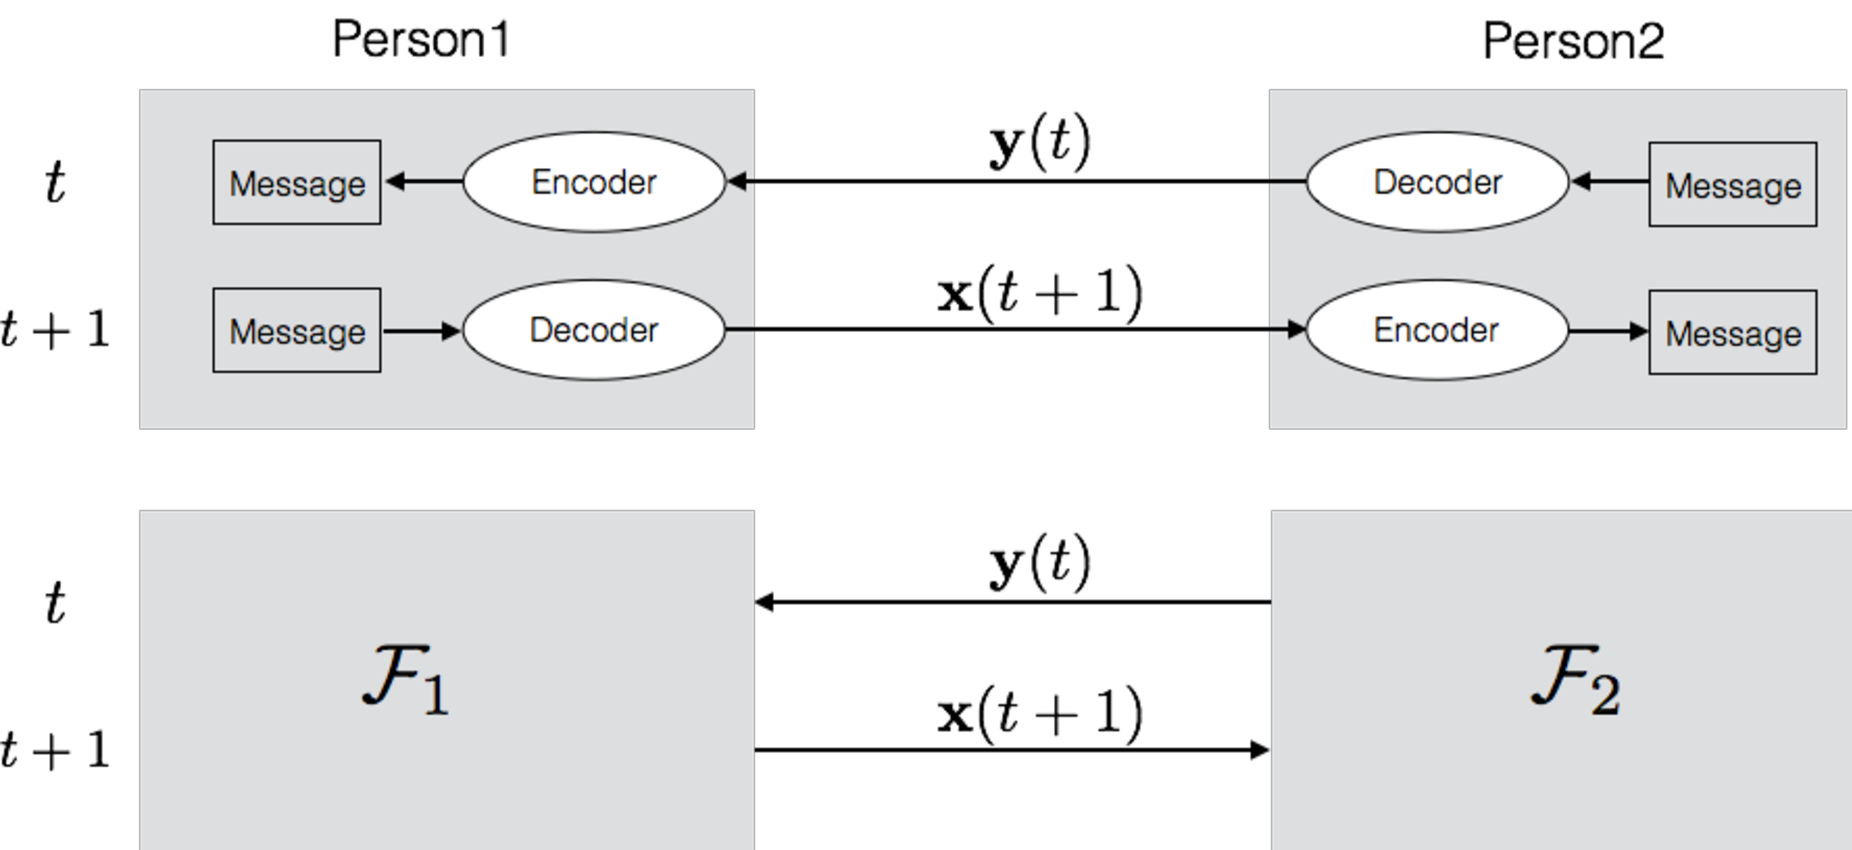
\includegraphics[trim=0 0 0 0, clip=true, width=0.5\columnwidth]{figures/encodDecod2}
%	
%	\caption{Encoder and Decoder model of Social Signals}	
%\end{figure}

%\begin{itemize}
%	\item Motivation: Nonverbal social signals play important role in social communication, transmitting rich information which cannot be conveyed by languages. 
%	\item They are still poorly understood. Why?
%	\item Challenges
%		\subitem - Measurement: large volume, occlusions, immense pose configuration, priming issue (requiring a markerless method).
%		\subitem - Understanding (prediction): high dimensional, hard to model by a hand-crafted way, no available large scale data for ``natural" social interactions, no previous work based on a data-driven method. 
%	\item Our approach
%		\subitem - We present a new capture system and method using massively multiple views: social interaction should be measured by fusing lots of (simple) measurements, rather than complicated methods with a few views
%		\subitem - We present a new data-driven method to model socially interacting multiple people's motion: the model should be trained using a large scale data capturing ``natural" social interactions
%
%\end{itemize}


%\section{Notation}

%During social communication, people use nonverbal body signals using their body movement and facial expression to transmit their intent and emotion. The convey signals have richer information which cannot be conveyed by just using verbal cues. This signal plays very important role, but poorly understood up to now. 

%
%Despite the fundamental role nonverbal cues play in enabling social function~\cite{Birdwhistell-1970,Philpott-1983}, the protocol underlying this communication is poorly understood---Sapir~\cite{Sapir-1949} called it ``an elaborate code that is written nowhere, known to no one, and understood by all". Some structures of this code have been identified through observational study, such as reciprocity~\cite{Brazelton-1974} or synchrony~\cite{Condon-1974}. However, systematic studies of such phenomena have remained almost entirely focused on the analysis of facial expressions, despite emerging evidence~\cite{Meeren-2005,Aviezer-2012} that facial expressions provide a fundamentally \emph{incomplete} characterization of nonverbal communication. One proximal cause for this singular focus on the face is that capturing natural social interaction presents challenges that current state-of-the-art motion capture systems simply cannot address. This paper describes an approach to capture social signals in natural human interactions, presenting fundamental innovations that span capture design architecture, motion reconstruction algorithms, and a large scale dataset capturing more than 3 hours of group interaction scenes using 521 heterogeneous sensors.
%
%There are four principal challenges in capturing social signaling between individuals in a group: (1) social interactions have to be measured over a volume sufficient to house a dynamic social group, yet subtle details of the motion where important social signals are embedded must be captured; (2) strong occlusions emerge functionally in natural social interactions (e.g., people systematically face each other while interacting, bodies are occluded by gesticulating limbs); (3) human appearance and configuration variation is immense; and (4) social signaling is sensitive to interference---for instance, attaching markers to the face or body, a pre-capture model building stage, or even instructing each individual to assume a canonical body pose during an interaction, primes the nature of subsequent interactions. 
%
%In this paper, we present a system designed to address these issues, with integrated innovations in hardware design, motion representation, and motion reconstruction. The organizing principle is that social motion capture should be performed by the consolidation of a large number of ``weak" perceptual processes rather than the analysis of a few sophisticated sensors. The large number of views provide robustness to occlusions, provide precision over the capture space, and facilitate the boosting of weak 2D human pose detectors into a strong 3D skeletal tracker without any prior about the scenes and subjects. In particular, our contributions include: 
%
%	1) \textbf{Modularized Hardware}: We present the modular design of a massively multiview capture consisting of 480 VGA cameras, 31 HD Cameras, and 10 Kinect v2 RGB+D sensors, distributed over the surface of geodesic sphere with a 5.49m diameter (sufficient to house social groups).  %simultaneously triggered/accurate time aligned
%	
%	2) \textbf{3D Motion Reconstruction Algorithm for Interaction Capture}:  We present a method to automatically reconstruct full body motion of interacting multiple people. Our method does not rely on a 3D template model or any subject-specific assumption such as body shape, color, height, and body topology. Yet, our method works robustly in various challenging social interaction scenes of arbitrary number of people, producing temporally coherent time-varying body structures. Furthermore, our method is free from error accumulation and, thus, enables capture of long term group interactions (e.g., more than 10 minutes). 
%	%Our system does not require subjects to: (1) perform any predefined pose for initial alignment; (2) wear clothings with distinctive color from others, (3) directly face sensors to get reasonable measurements; (4) restrict the in-group movement of subjects. All these benefits are key to enabling the study of social interactions at scale. 
%	
%%	3) \textbf{Skeletal Representation}: We present a new representation for social motion capture labeling and embedding a dense 3D trajectory stream within a moving skeletal frame for each individual.
%	%	\item \textbf{3D Motion Reconstruction Algorithm}: We present a novel algorithm, inspired by boosting approaches, for fusing ``weak" human pose detection in each view with 3D tracking, to estimate the articulated nonrigid representation across the diverse set of views
%	%Our algorithm is designed to capture the motion of arbitrary (unknown) number of multiple people, without making prior assumptions about the subjects such as their body shape, texture, and measurement of bone length. Thus, we do not require a predefined model for each individual, or require participants to assume a canonical body pose for initialization during capture. 
%	
%	3) \textbf{Social Interaction Dataset}: We publicly share a novel dataset which is the largest in terms of the number of views (521 views), duration (3+ hours in total), and the number of subjects in the scenes (up to 8 subjects) for full body motion capture. Our dataset is distinctive from the previously presented datasets in that ours captures natural interactions of groups without controlling their behavior and appearance and contains motions with rich social signals as shown in Figure~\ref{fig:iconicPoses} (right). The system described in this paper provides empirical data of unprecedented resolution with the promise of facilitating data-driven exploration of scientific conjectures about the communication code of social behavior. All the data and output are publicly shared on our website\footnote{ \url{https://domedb.perception.cs.cmu.edu}}. 
%	
	
%	
%\section{Proposal Summary}
%\subsection{Completed Work to Data}
%\subsection{Proposed Work}
%\subsection{Timeline}
%\section{Notations}
%
%\section{Multiview System}
%\section{Markerless Motion and Face Capture}
%\section{Social Signal Processing}
%\section{Overview of Contributions}
%\subsection{Timeline}
%\begin{figure}[!ht]
%	\centering
%	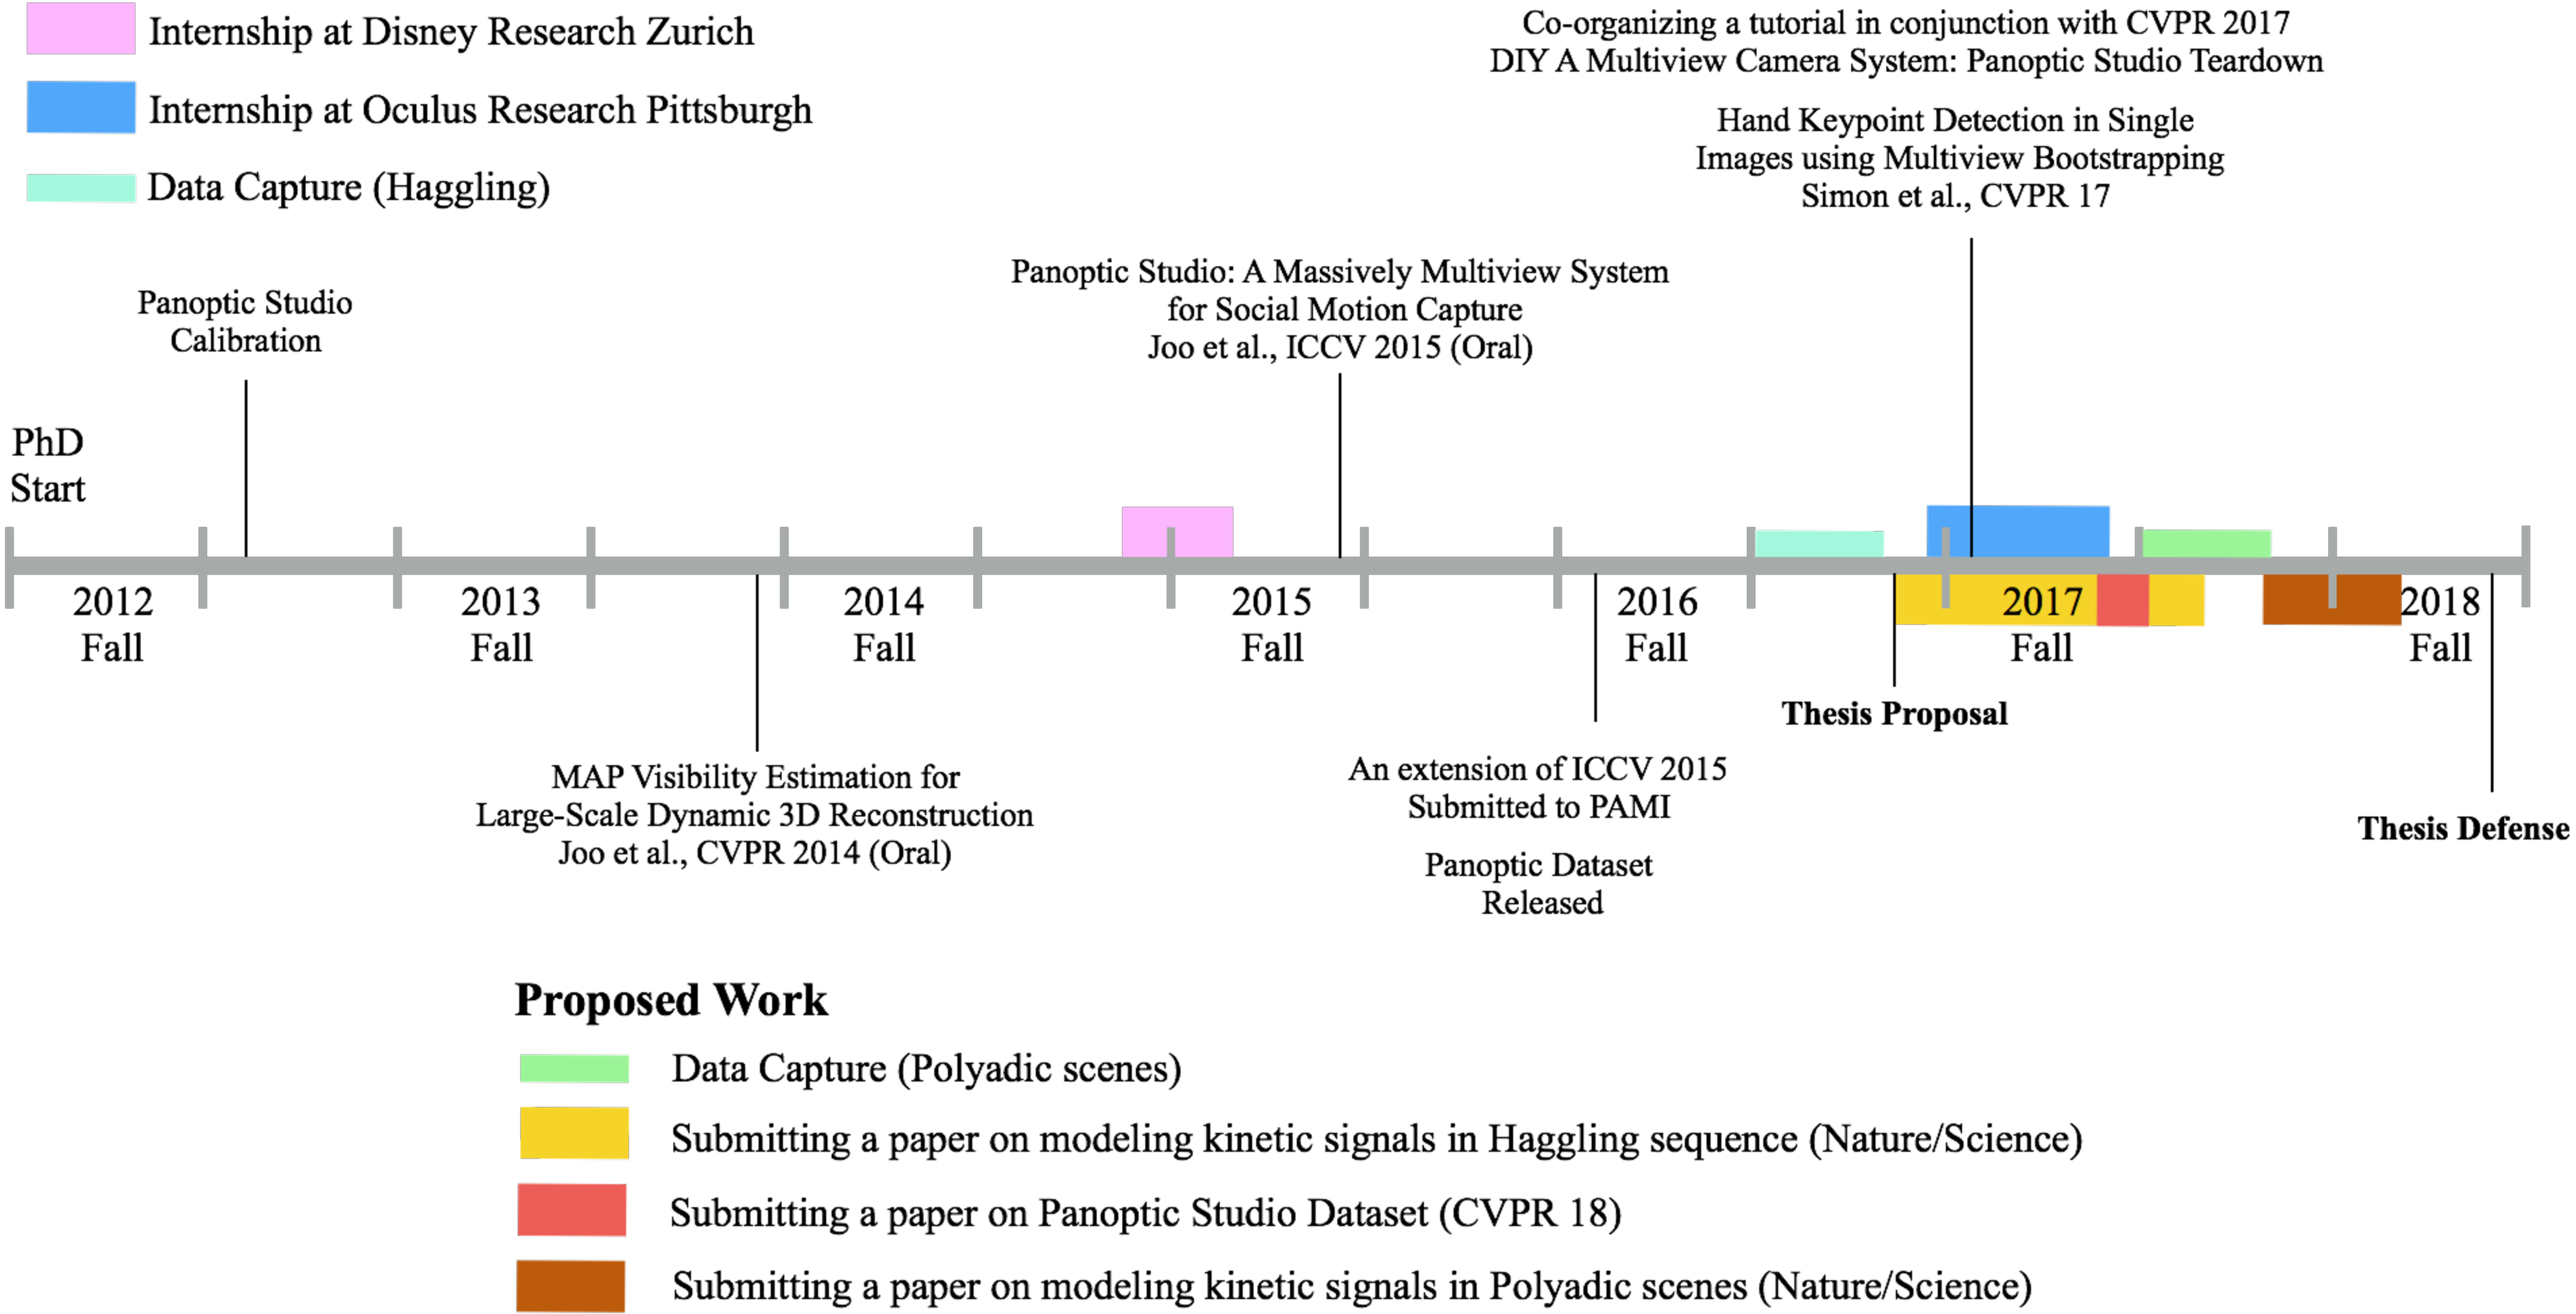
\includegraphics[trim=0 0 0 0, clip=true, width=0.95\textheight,angle=270,origin=c]{figures/timeline}
%%	\caption{A Timeline}	
%	\label{fig:timeline}
%\end{figure}

\newpage 

%%	
%%
	\part{Sensing Social Signals}
	% !TEX root = ../thesis.tex

%
%
%\chapter{The Panoptic Studio: A Massively Multiview Capture System}
%\section{Modularized Hardware Design}
%\subsection{Structure}
%\subsection{Architecture}
%\section{Calibration}
%\subsection{Temporal Calibration}
%\subsection{Spatial Calibration}
%\section{Capture Procedures}
%
%\chapter{Methods For Social Interaction Capture}
%\section{Dense Trajectory Stream Reconstruction}
%\section{Markerless Social Interaction Capture}
%\subsection{Body}
%\subsection{Face}
%\subsection{Hand}
%\section{Motion Refinement to Capture Subtle Details (Proposed)}
%\section{Panoptic Studio Dataset}


\chapter{The Panoptic Studio}%: A Massively Multiview System}
\label{chapter:system}

There are principal challenges in capturing social signals between individuals in a group: (1) social interactions have to be measured over a volume sufficient to house a dynamic social group, yet subtle details of the motion where important social signals are embedded must be captured; (2) strong occlusions emerge functionally in natural social interactions (e.g., people systematically face each other while interacting, bodies are occluded by gesticulating limbs); (3) human appearance and configuration variation is immense; and (4) social signaling is sensitive to interference---for instance, attaching markers to the face or body, a pre-capture model building stage, or even instructing each individual to assume a canonical body pose during an interaction, primes the nature of subsequent interactions. 

The Panoptic Studio is developed to overcome these challenges. The system has a large geodesic sphere structure with a 5.49m diameter, with heterogeneous sensors on its surface including 480 VGA cameras, 31 HD cameras, 10 RGB+D sensors, 23 microphones, and 5 DLP projectors. The core principle and motivation in building this system is to obtain as much measurement as possible to have minimum assumptions about the scenes. We found that the large number of views of the system greatly releases all the aforementioned sensing challenges, and also enables us to use relatively ``weak" perceptual processes from the large number of views 	rather than a complicated method with strong assumptions about the scenes. To this end, this system enables us to measure the full spectrum social signals of naturally interacting groups. This chapter covers the various hardware and low-level software issues in building the Panoptic Studio, including structure design, architectures, synchronization, and spatial calibration.  

The Panoptic Studio is the output of several years of collaboration with Tomas Simon, Xulong Li, Hao Liu, Lei Tan, Lin Gui, Timothy Godisart, Sean Banerjee, Hyun Soo Park, Iain Matthews, Bart Nabbe, Shohei Nobuhara, Takeo Kanade, and Yaser Sheikh. 
%do not introduce any kind of sight restriction on the subjects
%Why not using just 100 HD instead of this combination?)
%Modularized design is the key (same number of cameras, HD on the center). 

% Modularized design, VGA, HD, Kinect
\section{Structural Design}
% Add optimization routine
The physical frame of the studio is a variant of a face-transitive solid called a truncated pentagonal hexecontahedron. This particular structure was selected because it has among the largest number of transitive faces of any geodesic dome~\cite{Williams1979}. The transitivity of the faces enables the modular architecture, and ensures that the structure remains easy to upgrade and customize with different panels of the same configuration. The structure has a diameter of 5.49m and a total height of 4.15m. The floor of the dome is 1.40m below the center of the sphere structure to increase access to the edges. In all, the structure consists of 6 pentagonal panels, 40 hexagonal panels, and 10 trimmed base panels. The interior and exterior view of the Panoptic Studio are shown in Figure~\ref{fig:dome_ext_int} and a 360\degree~panoramic view of the interior of the Panoptic Studio is shown in Figure~\ref{fig:dome_panorama}. The structural design is illustrated in the left of Figure~\ref{fig:dome_structure}.


\begin{figure}
	\centering       
	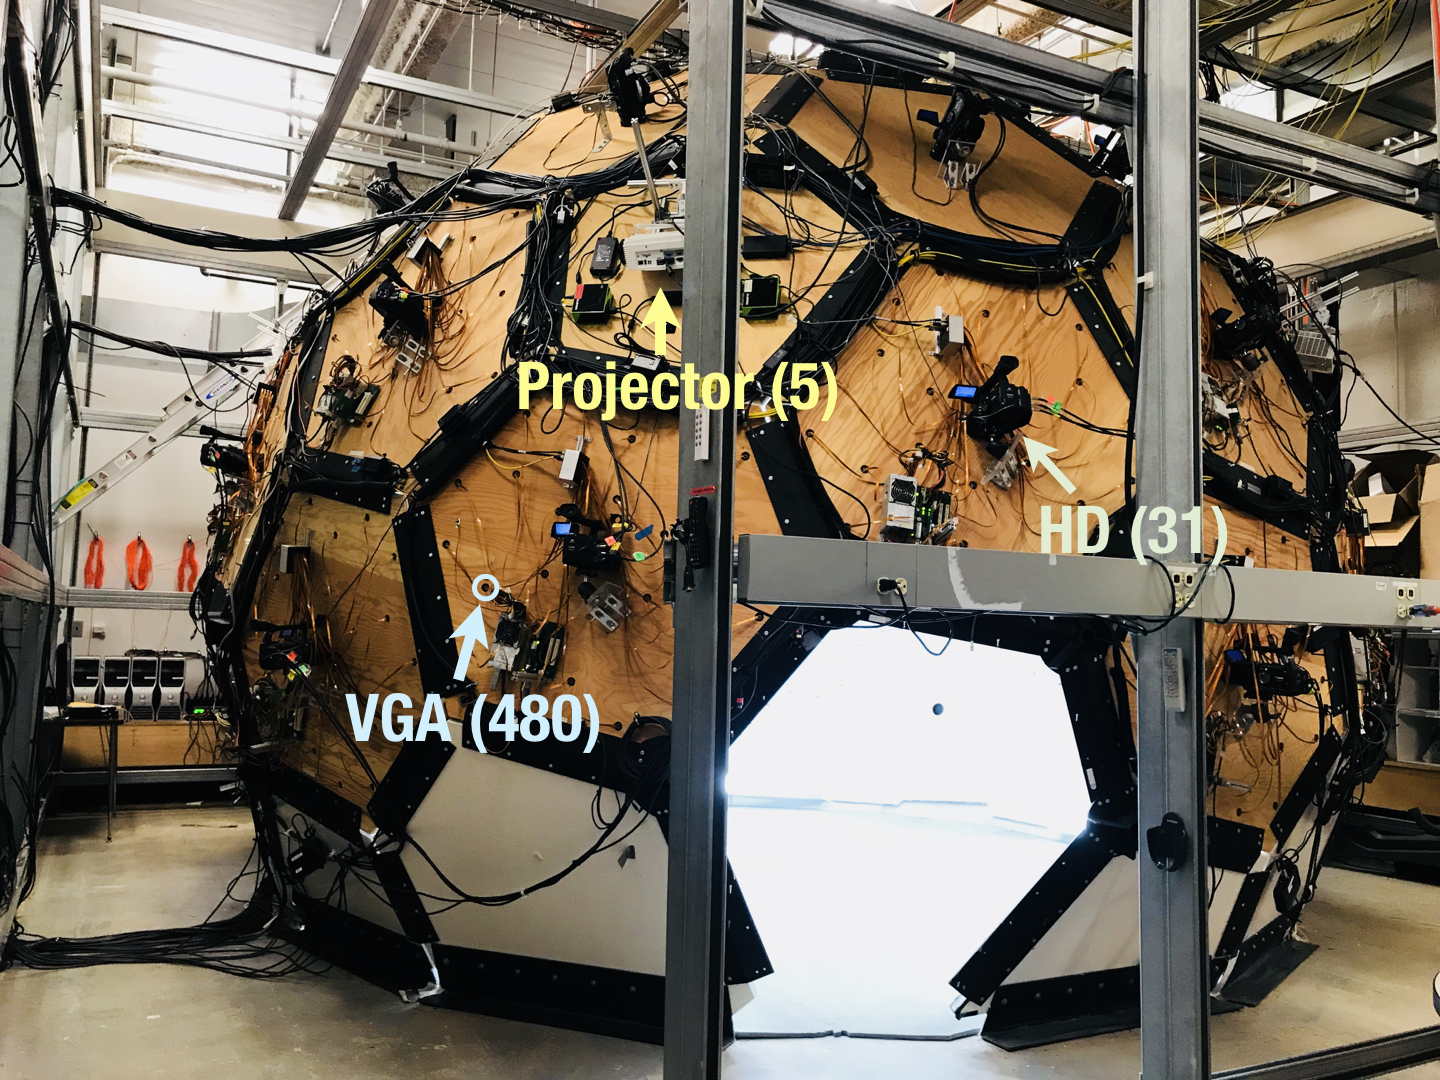
\includegraphics[trim=0 0 0 0,clip,width=\linewidth]{fig_system/dome_exterior2_label}
	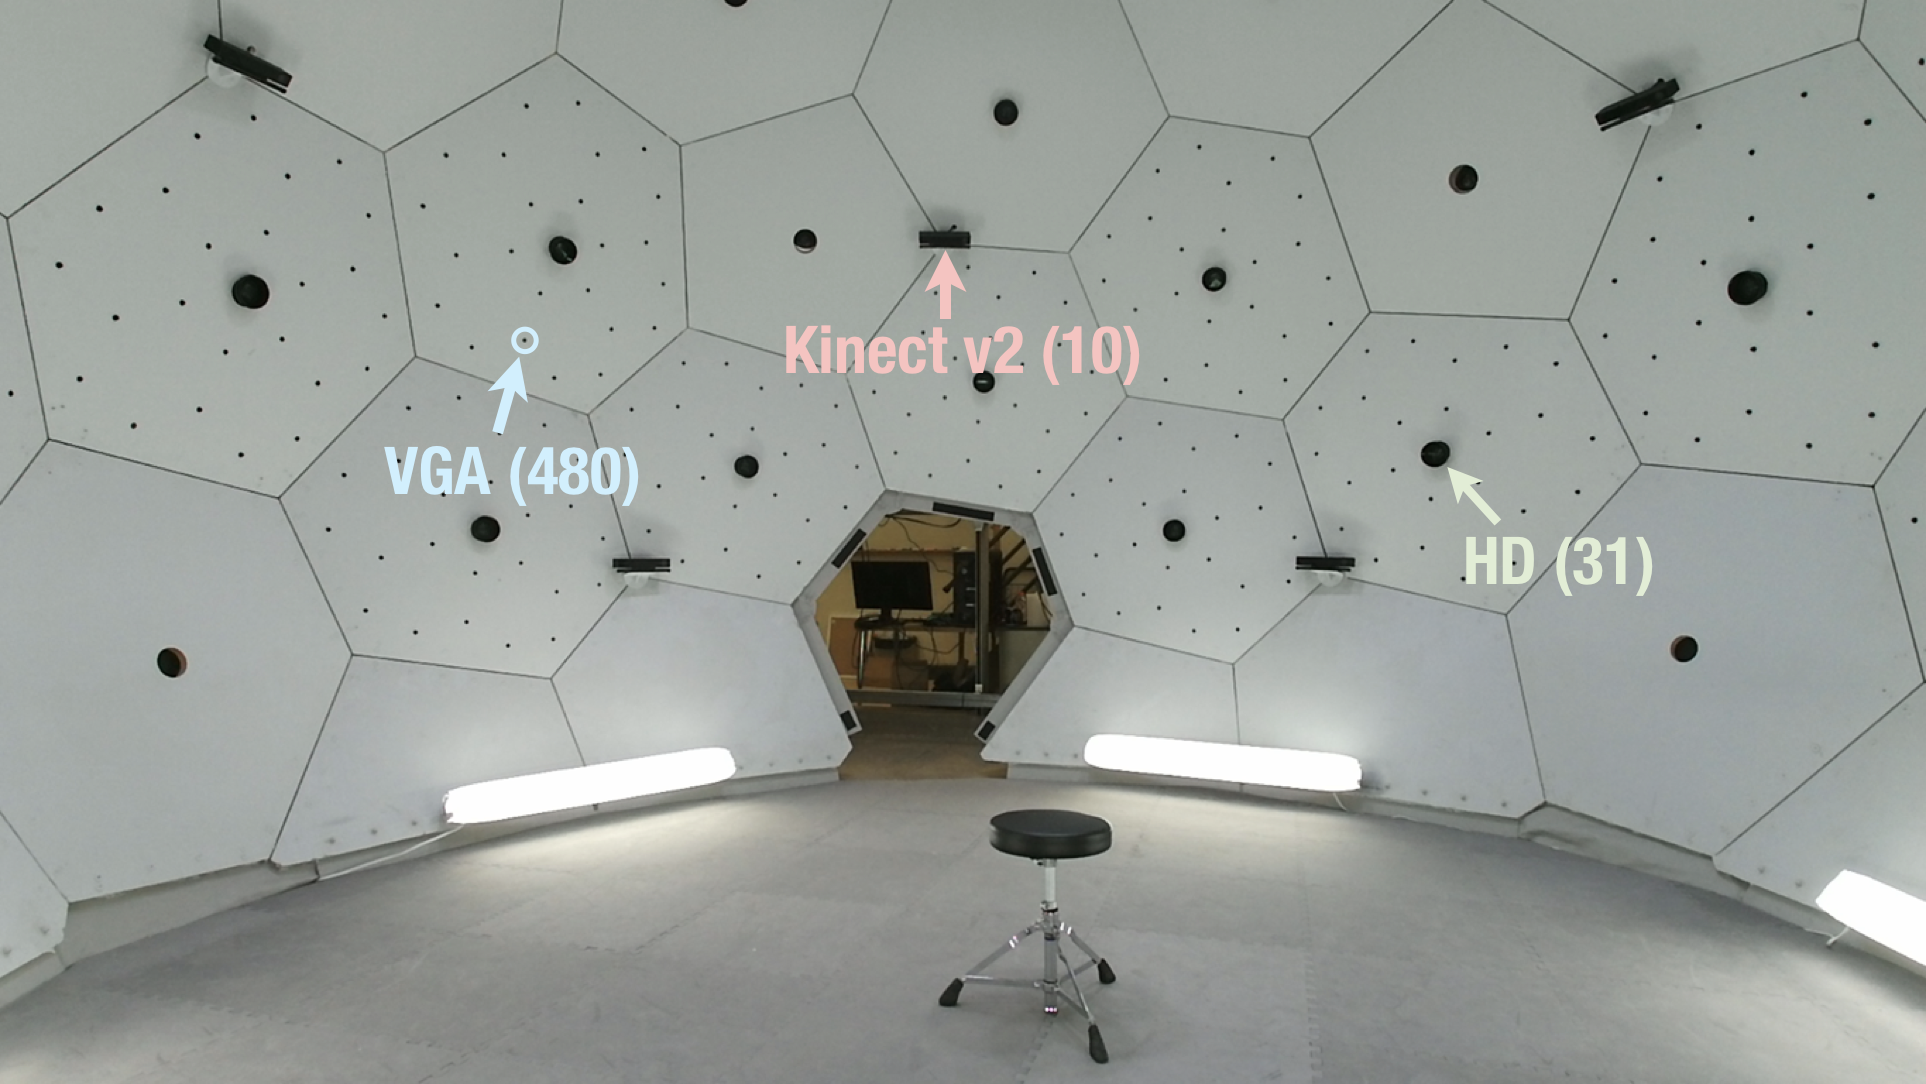
\includegraphics[trim=0 0 0 0,clip,width=\linewidth]{fig_system/panoptic_inside}	
	\caption{The exterior and interior shape of the Panoptic Studio, equipped with  480 VGA cameras, 31 HD cameras, 10 RGB+D cameras, and 5 DLP Projectors. (Top) The exterior of the Panoptic Studio. (Bottom) The interior of the Panoptic Studio.} 
	\label{fig:dome_ext_int}
\end{figure}

\begin{figure}
	\centering       
	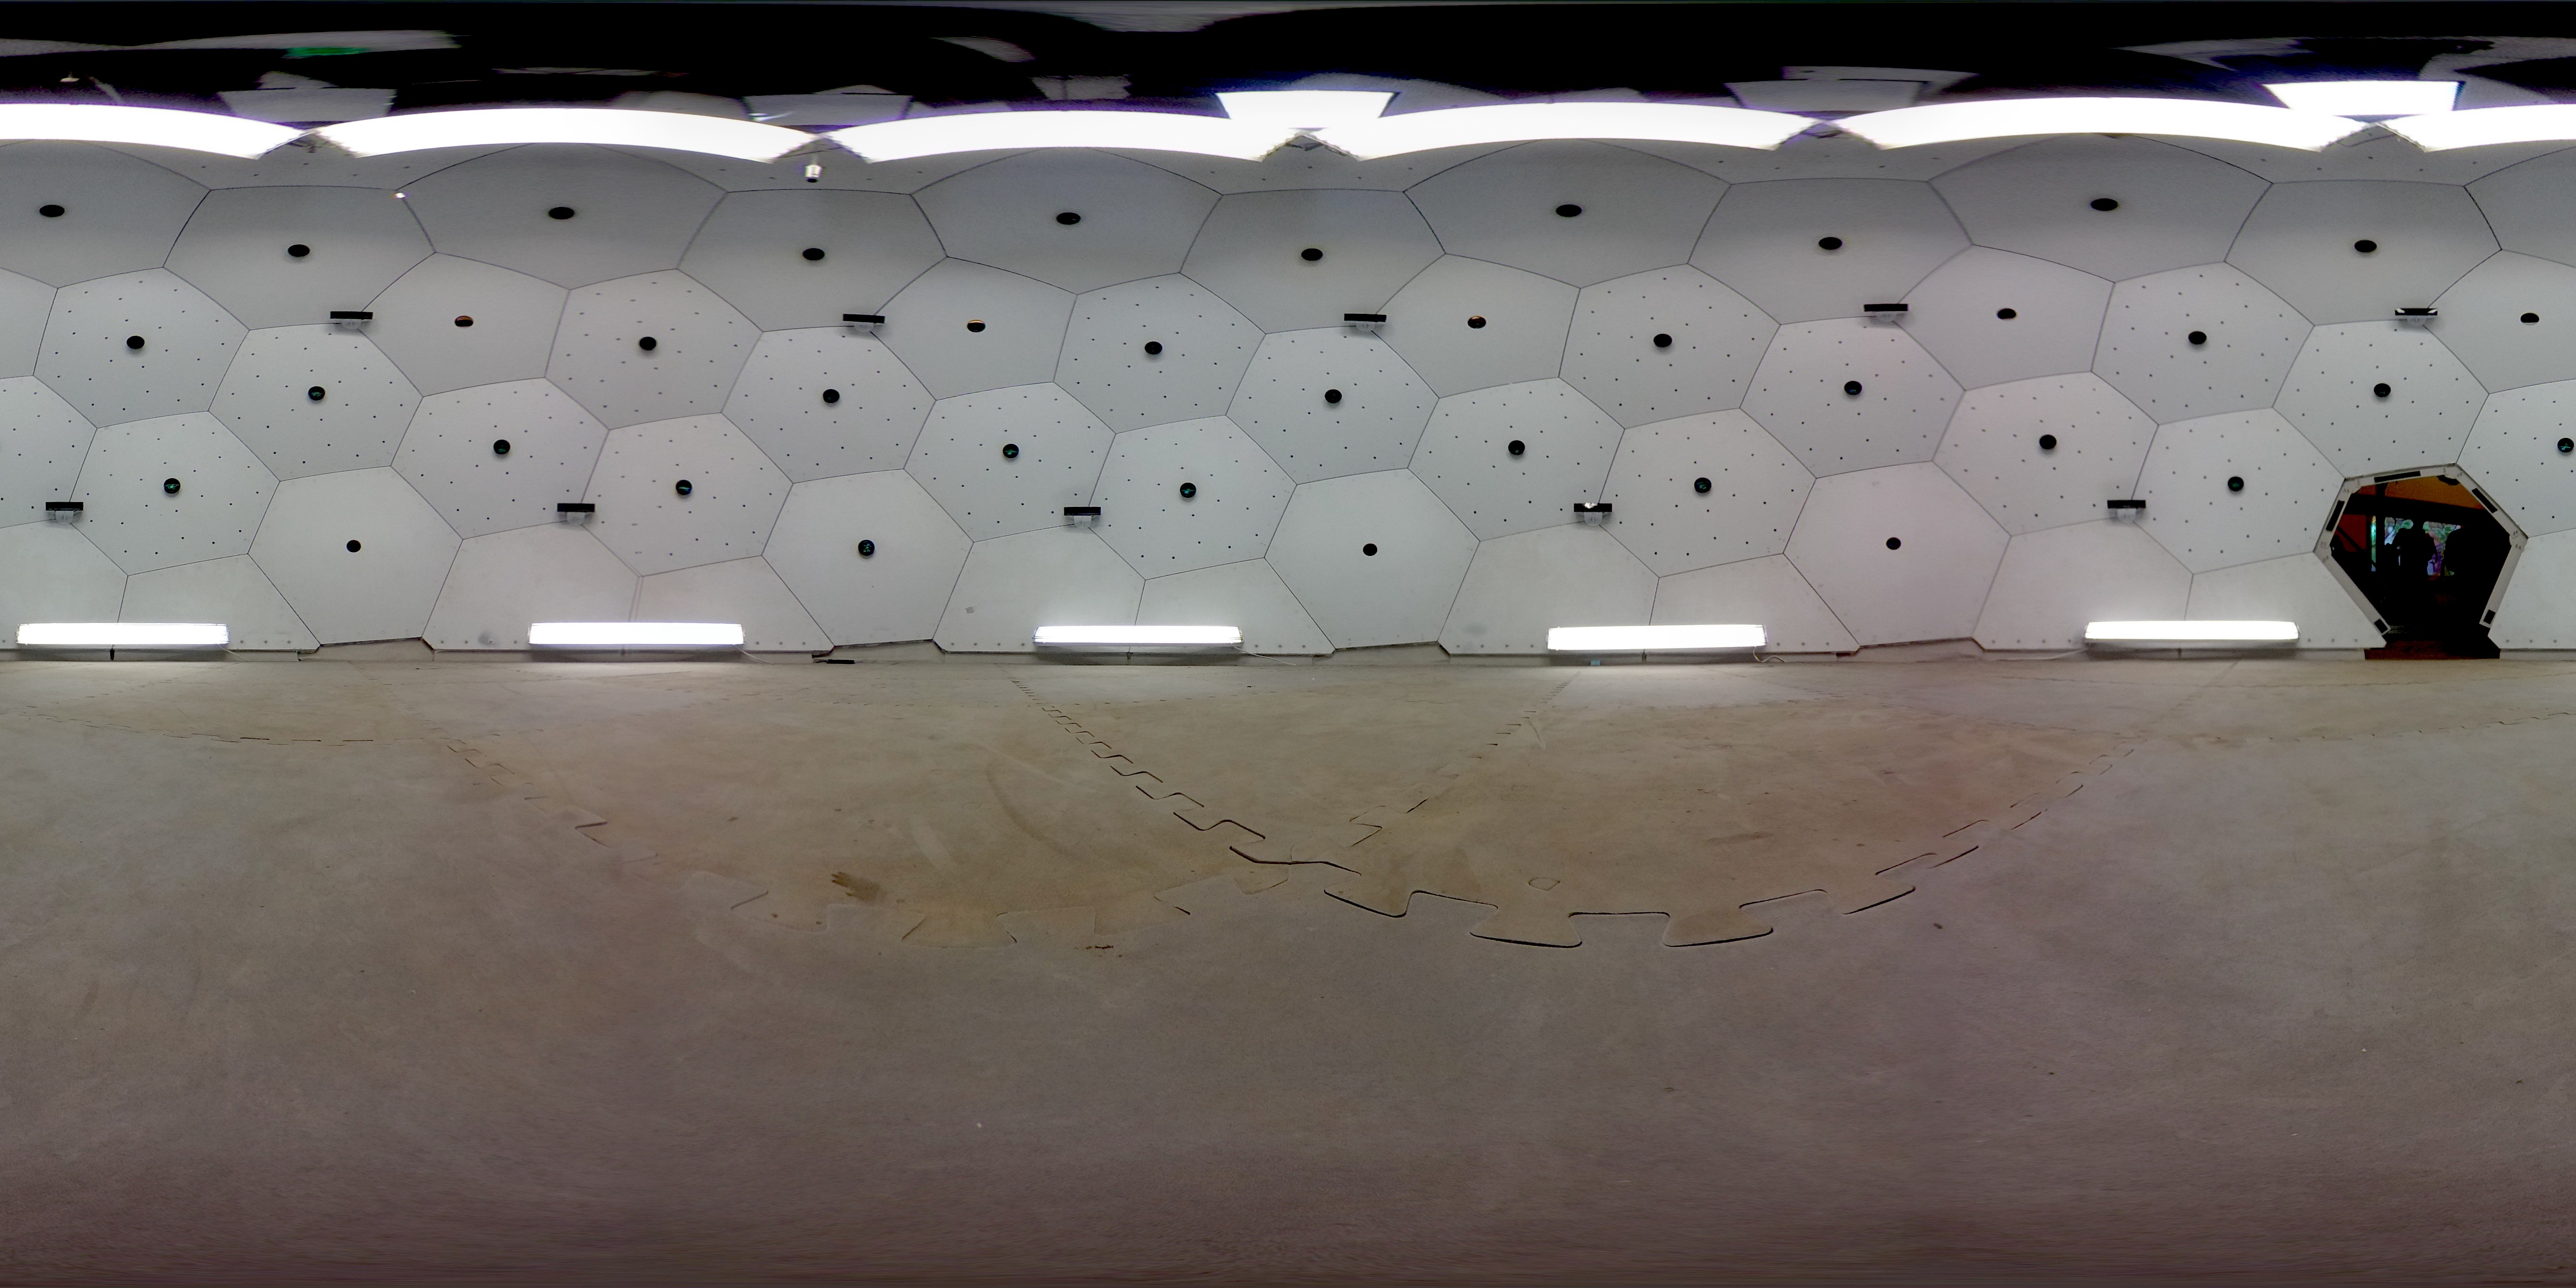
\includegraphics[trim=0 0 0 0,clip,width=\linewidth]{fig_system/dome_pano}	
	\caption{A 360\degree~panoramic photo captured inside the Panoptic Studio. The empty panel is the entrance of the Studio.} 
	\label{fig:dome_panorama}
\end{figure}

\begin{figure}
	\centering       
	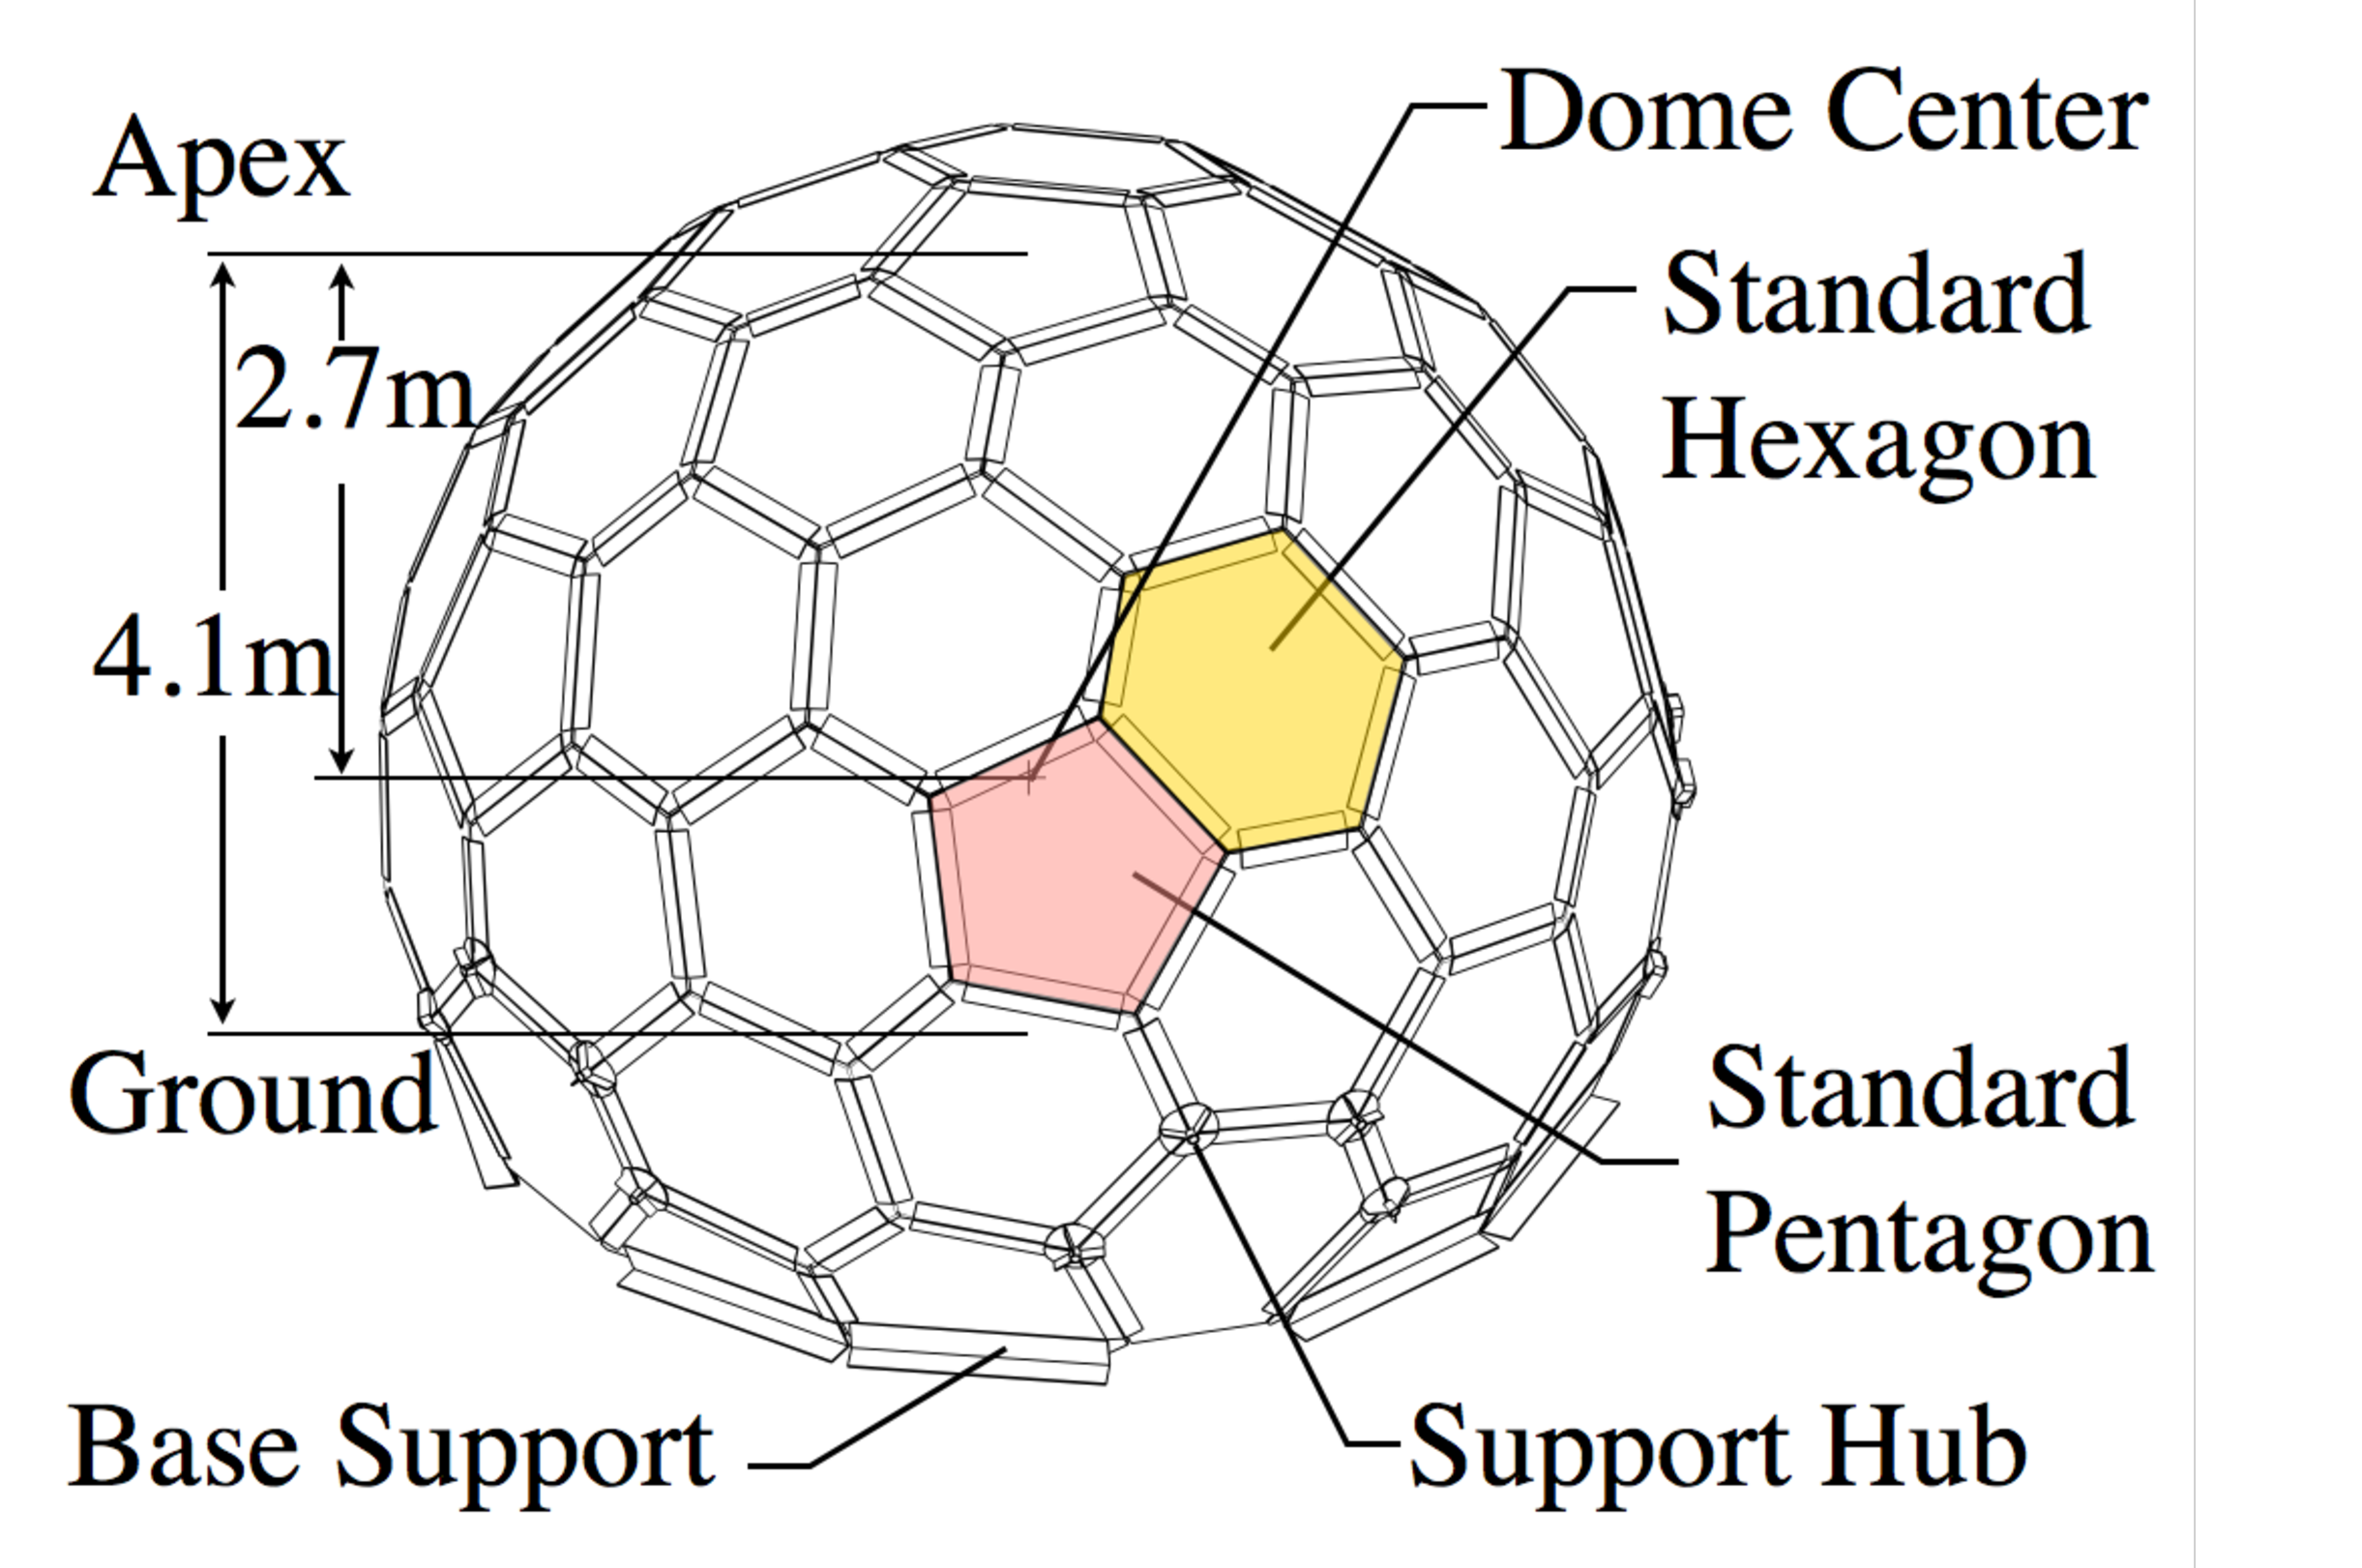
\includegraphics[trim=0 0 100 0,clip,width=0.48\linewidth]{figures/DomeFigure2} 
	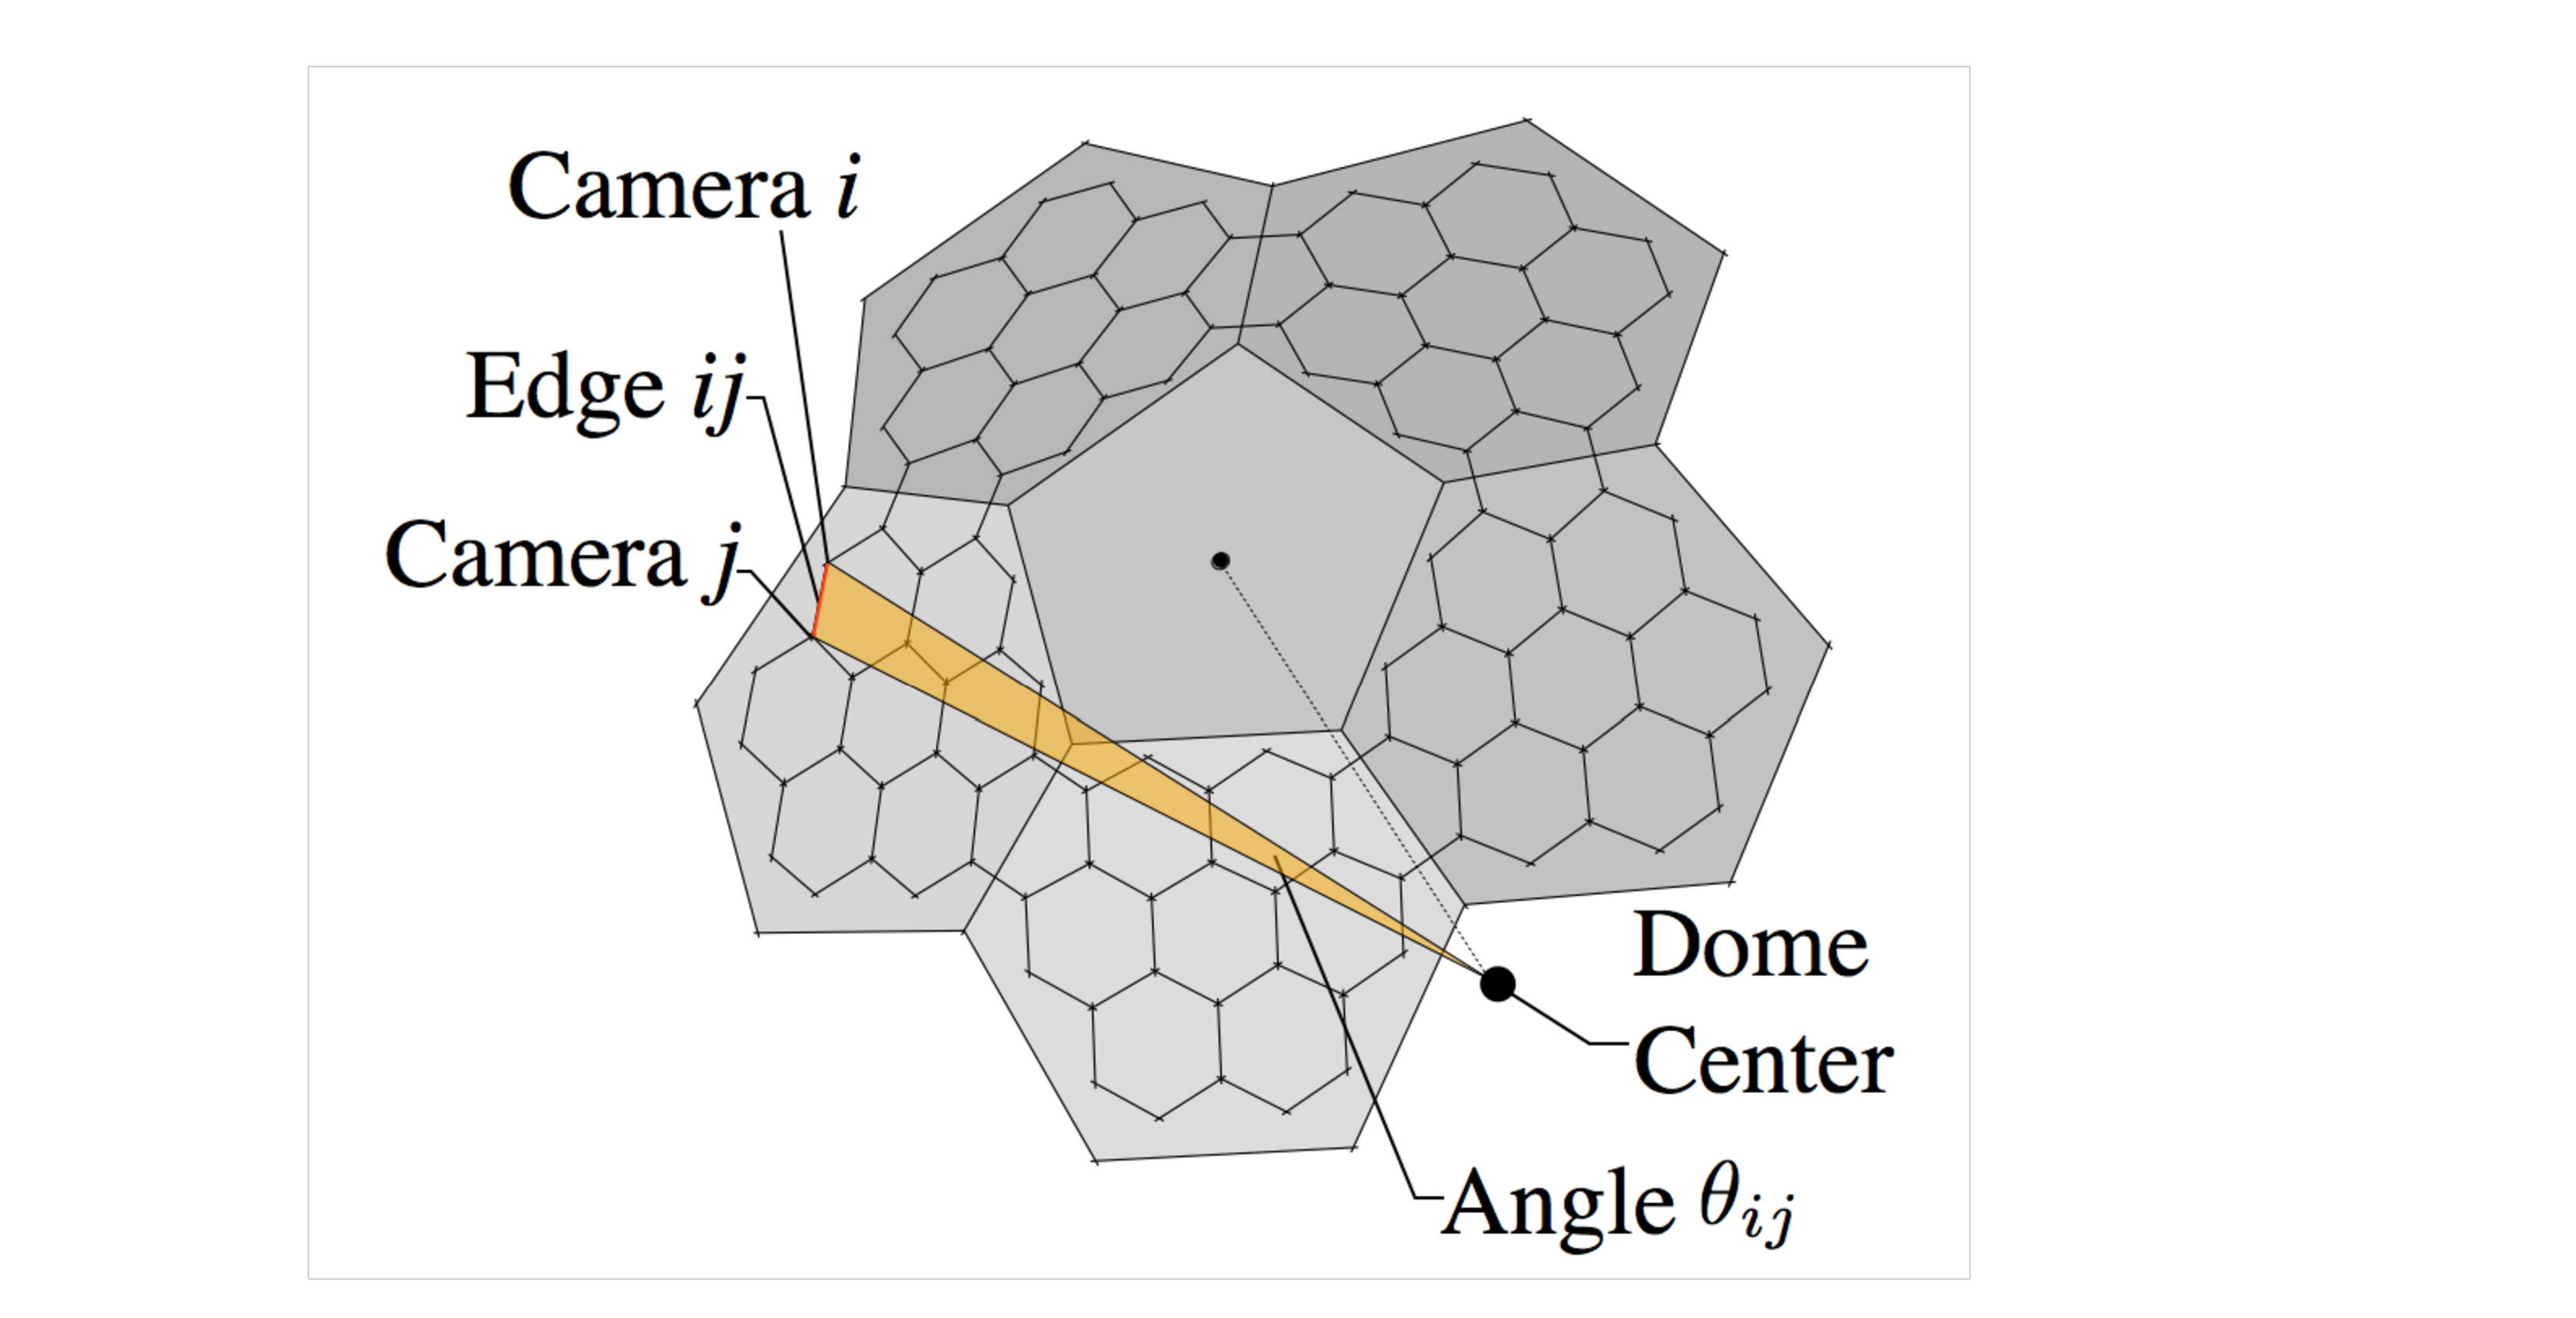
\includegraphics[trim=230 50 400 50,clip,width=0.48\linewidth]{figures/DomeFigure3}
	\caption{Structural Design of the Panoptic Studio (Left) The system has a modularized design with repeated pentagon and hexagon shapes, to ensure interchangeability (Right) Optimized VGA camera positions to ensure uniform angles with respect to the dome center between each camera and all its neighbors (e.g., Camera $i$ is a neighbor of Camera $j$).} 
	\label{fig:dome_structure}
\end{figure}


Our design was modularized so that each hexagonal panel houses a set of 24 VGA cameras and a HD camera. To determine the placement of the VGA cameras, we initialized their positions by tessellating the hexagon face into 24 triangles and using this initialization to define a 3-neighborhood structure shown in the right of Figure~\ref{fig:dome_structure}. Using this neighborhood structure and the initialization we determine the placement of the cameras over the geodesic dome by minimizing the difference in angles between all neighbors of every camera,

{\small
	\begin{equation}\nonumber
	\{\theta_{ij}\}^* = \arg \min_{\{\theta_{ij}\}} \sum_{p=1}^P \sum_{i=1}^{N} \sum_{j \in \mathcal{N}(i)}  \sum_{k \in \mathcal{N}(i) \neq j}  (r(\theta_{ij}|p)-r(\theta_{ik}|p))^2 ,
	\end{equation}
}where $P=20$ is the number of panels, $N=24$ is the number of cameras in each panel, $\mathcal{N}(\cdot)$ is the neighborhood of a camera, $r(\cdot|p)$ is a function transforming the angle on a reference panel to the $p$-th panel. The cameras sample the span of the vertical axis of the space and sample $48.71^\circ$ of the horizontal axis. With this distribution, the minimum baseline between any VGA camera and its nearest three neighbors is 21.05cm. 
	
The 31 HD cameras are installed at the center of each hexagonal panel, and 5 projectors are installed at the center of each pentagonal panel\footnote{Note that no sensors are installed on some panels (e.g., ceiling panels occluded by lights).}. Additionally, a total of 10 Kinect v2 RGB+D sensors are mounted at heights of 1 and 2.6 meters, forming two rings with 5 evenly spaced sensors each. %The interior and exterior of our system are shown in Figure~\ref{fig:domeFigure}, and components of our system is shown in Figure~\ref{fig:domeEquipment}


		 %Naturally, there is some variation in this number due to the physical imprecision of mounting.
	%Placement of cameras.
	%Williams, Robert (1979). The Geometrical Foundation of Natural Structure: A Source Book of Design. Dover Publications, Inc. ISBN 0-486-23729-X. (Section 3-9)
	% \noindent \textbf{Acquisition Hardware.} The dome has twenty panels, each with 24 VGA cameras and one HD camera, for a total for 480 VGA cameras and 16 HD cameras. The sensors are arranged to lie uniformly around the twenty panels. 
	
%	\begin{figure}
%	\centering       
%	%	\subfigure{\label{fig:domeFigure1}\includegraphics[trim=400 0 150 0,clip,width=0.45\linewidth]{imgs/Dome_outside}} 
%	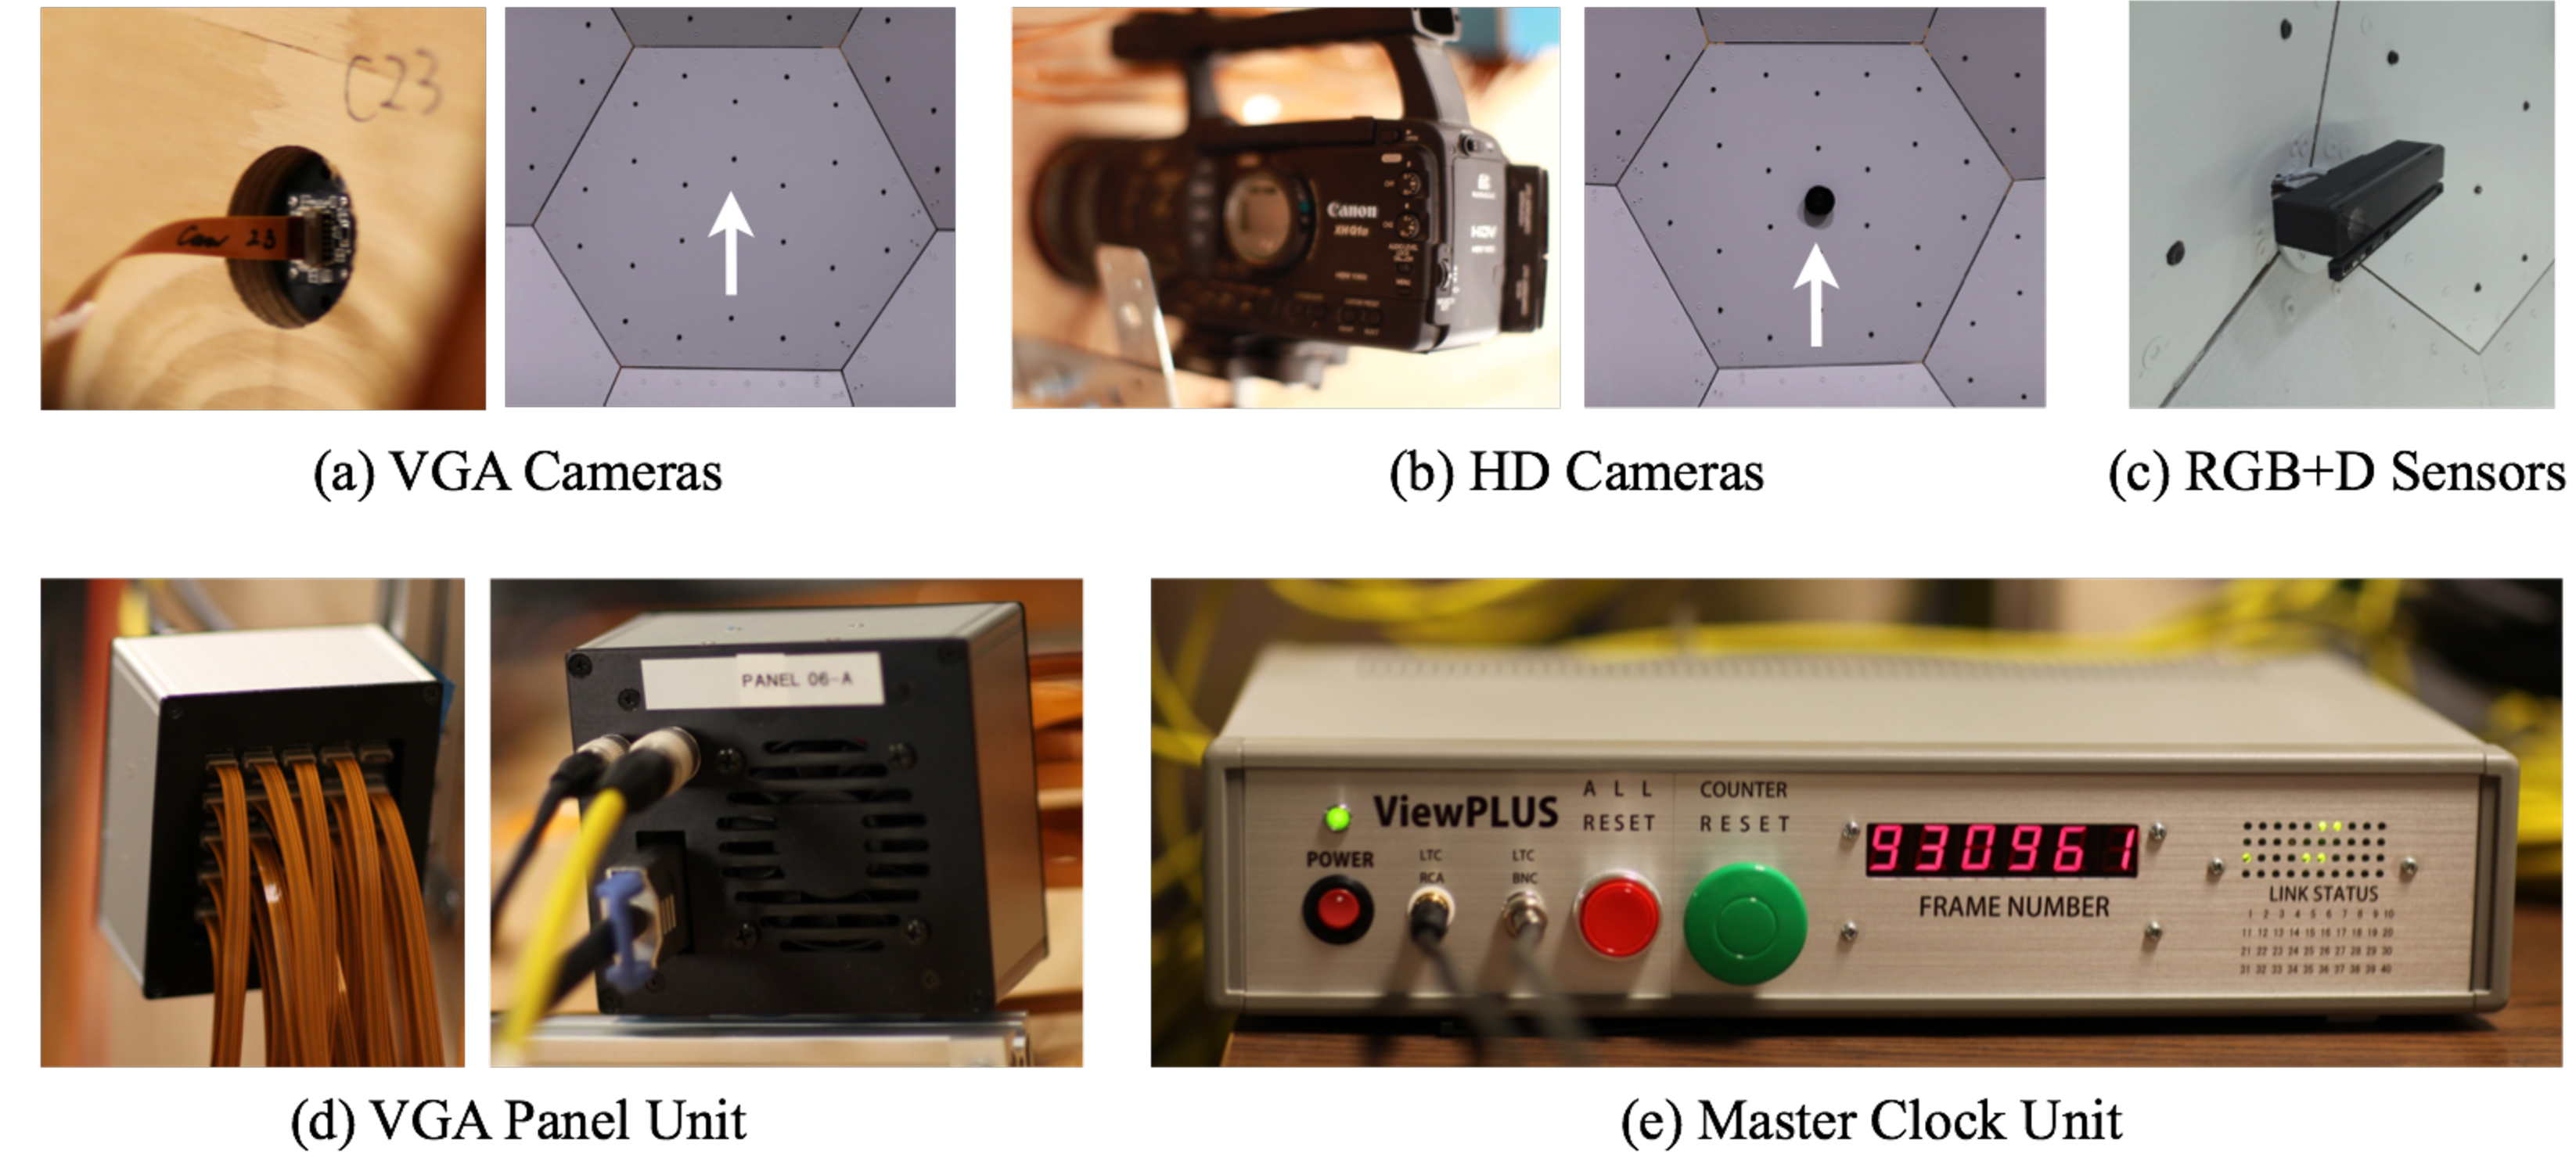
\includegraphics[trim=0 0 0 0,clip,width=\linewidth]{figures/Equipment}
%	\caption{Sensors and equipments installed in the Panoptic Studio. } 
%	\label{fig:domeEquipment}
%\end{figure}
\section{System Architecture}
%which consists of 480 VGA cameras, 31 HD cameras, 10 Kinect v2 RGB+D sensors, and 5 DLP projectors. 
Figure \ref{fig:dome_architecture} shows the architecture of our system. The panoptic studio is composed of four sub-systems: VGA camera system, HD camera system, RGB-D camera system, and projector system.

\noindent \textbf{VGA Camera System:} The 480 cameras are arranged modularly with 24 cameras in each of 20 standard hexagonal panels on the dome. Each module in each panel is managed by a Distributed Module Controller (DMC) that triggers all cameras in the module, receives data from them, and consolidates the video for transmission to the local machine. Each individual camera is a global shutter CMOS sensor, with a fixed focal length of 4.5mm, that captures VGA ($640\times480$) resolution images at 25Hz. The detailed configuration is shown in Figure~\ref{fig:dome_vgaSystem}. 

\begin{figure}[t]
	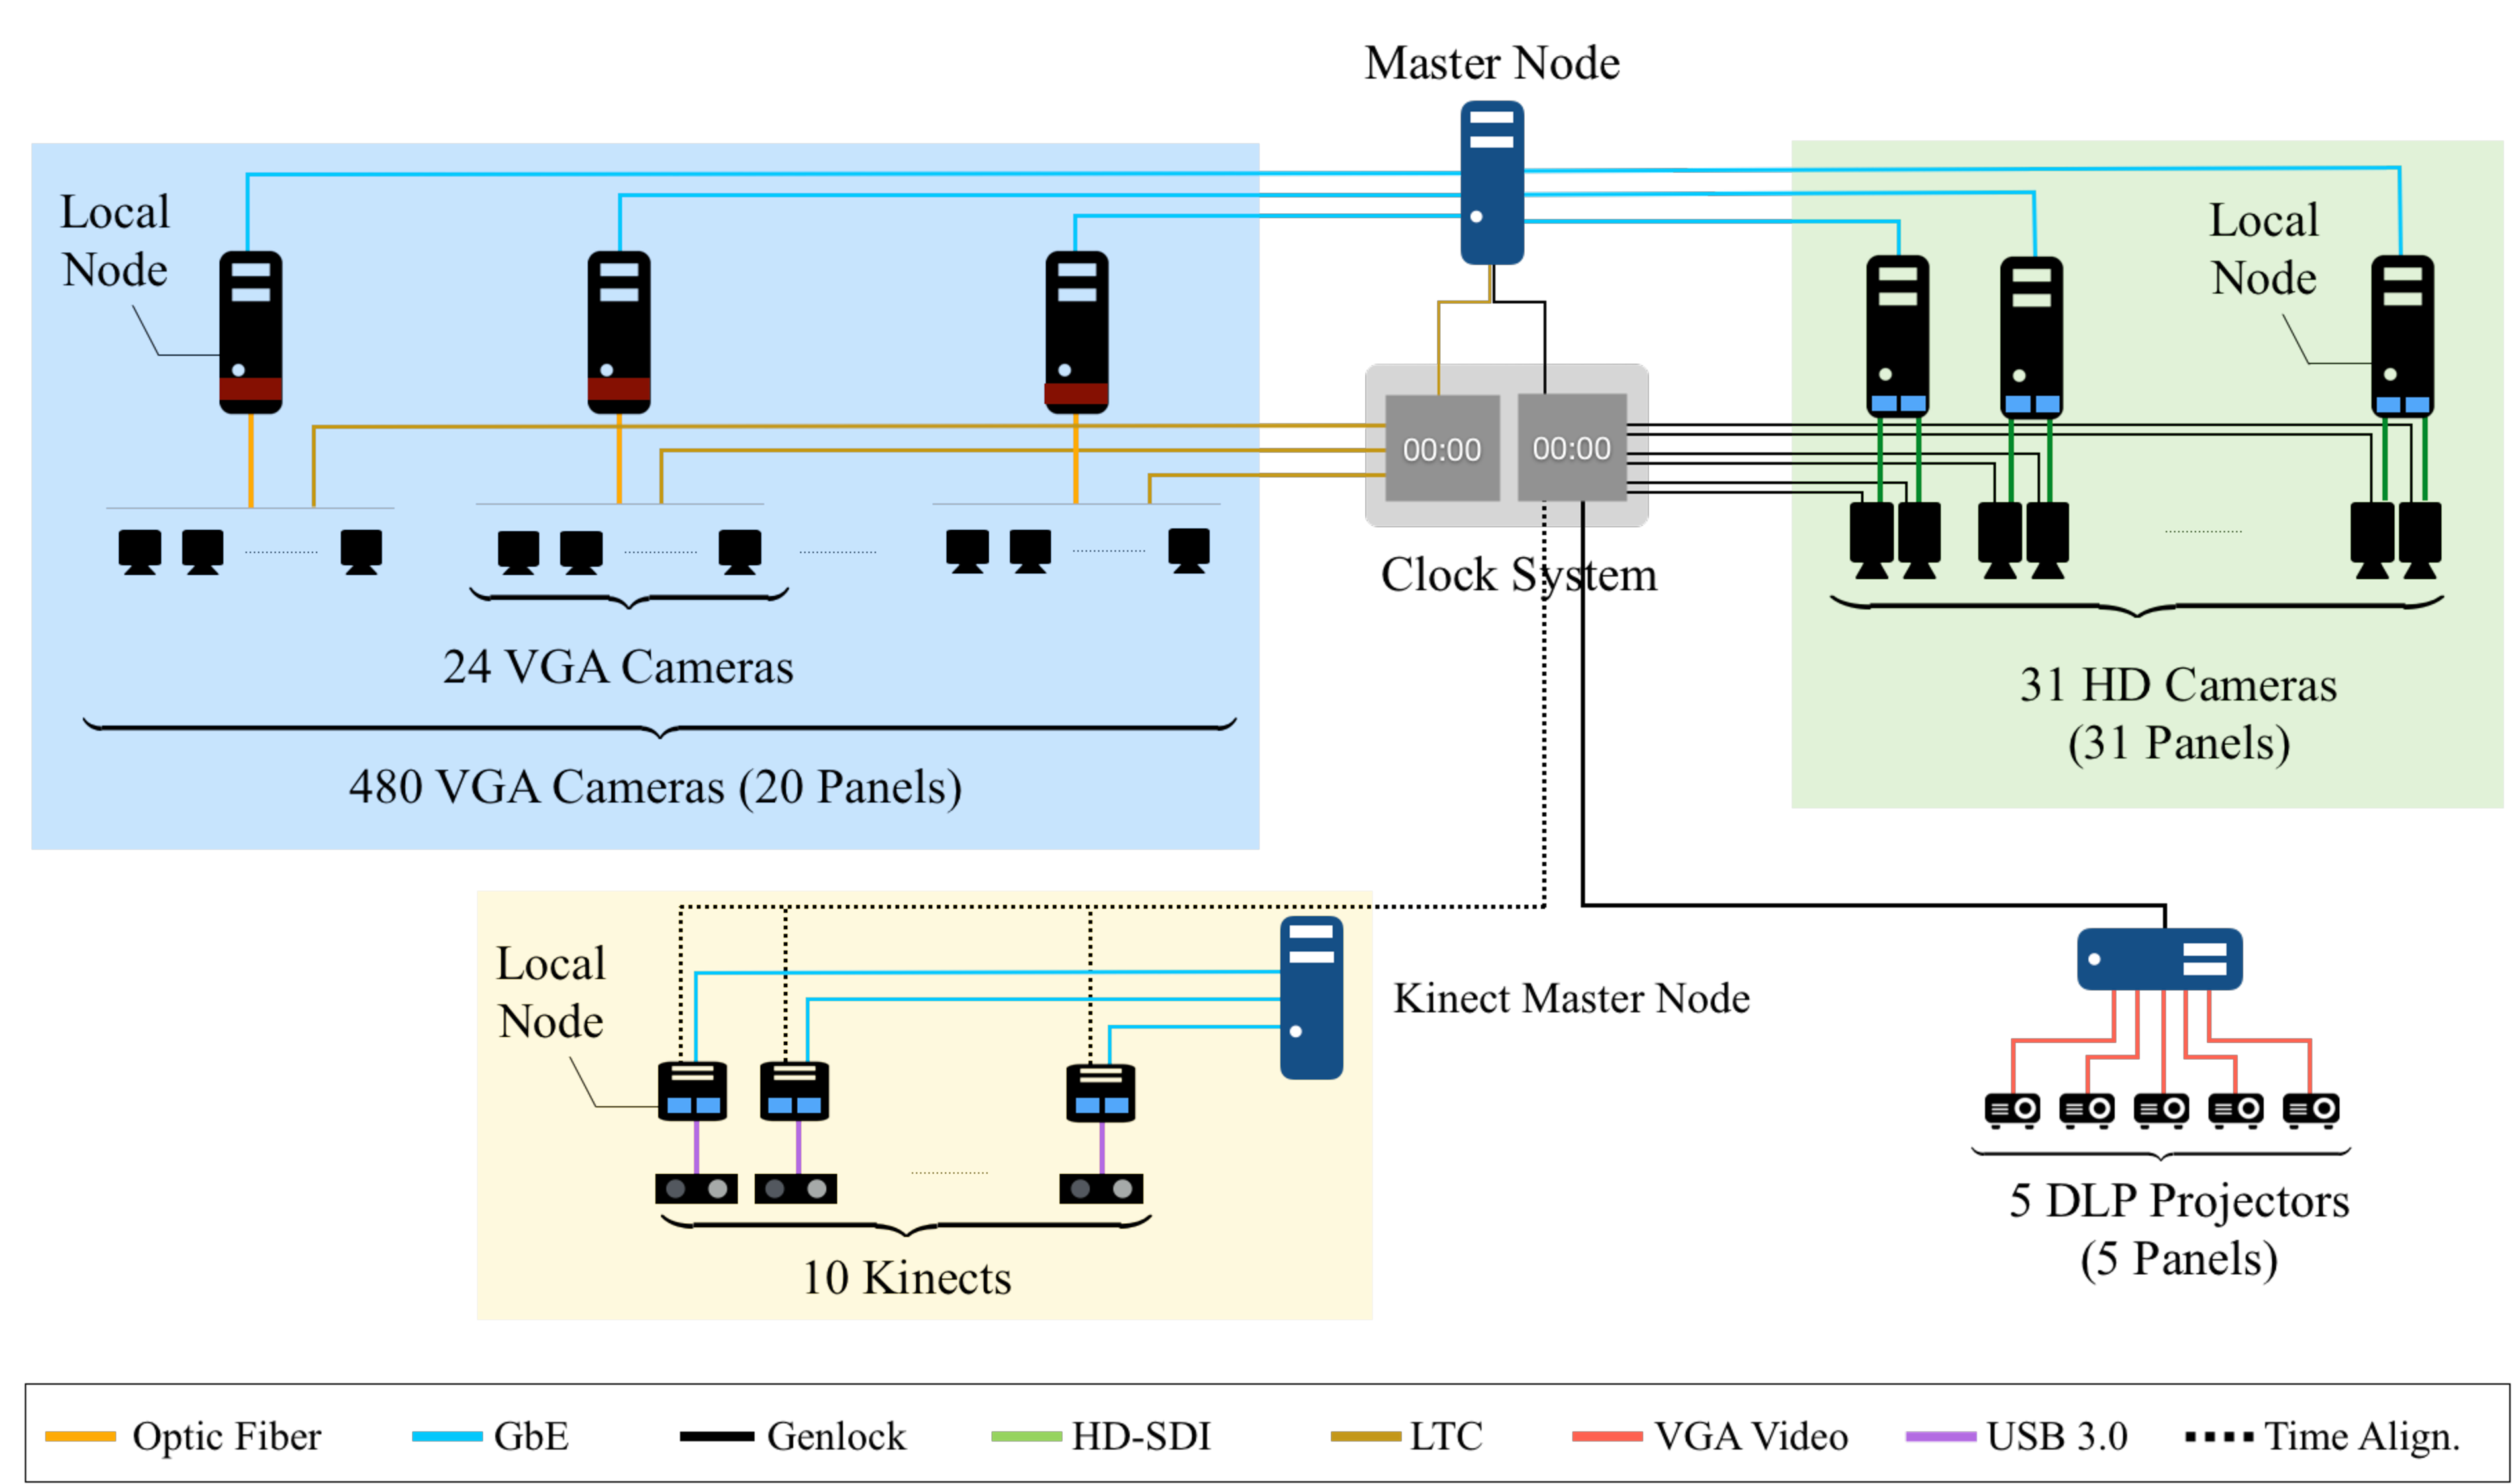
\includegraphics[width=\linewidth]{fig_system/panoptic_architecture}
	%\includegraphics[width=\linewidth]{images/Design6.pdf}
	%	\vspace{-0.2in}
	\caption{Modularized system architecture. The system is composed of four sub-systems, depending on sensor types. The studio houses 480 VGA cameras, 31 HD cameras, 10 RGB+D sensors, and 5 DLP projectors. The 480 VGA cameras are synchronized by a clock system with 25 Hz, and HD cameras and projectors are synchronized by another clock system with 29.97 Hz. Both clocks are temporally aligned by recording them as a stereo signal. 10 RGB-D sensors are also time-aligned in the common time domain. All the sensors are spatially calibrated to the same coordinate system.}
	\label{fig:dome_architecture}
\end{figure}

Each panel produces an uncompressed video stream at 1.47 Gbps, and thus, for the entire set of 480 cameras the data-rate is approximately 29.4 Gbps. To handle this stream, the system pipeline has been designed with a modularized communication and control structure. For each module, the clock generator sends a frame counter, trigger signal, and the pixel clock signal to each DMC associated with a panel. The DMC uses this timing information to initiate and synchronize capture of all cameras within the module. Upon trigger and exposure, each of the 24 camera heads transfers back image data via the camera interconnect to the DMC, which consolidates the image data and timing from all cameras. This composite data is then transferred via optical interconnect to the module node, where it is stored locally. The 20 local nodes for VGA camera system are shown in left of the Figure~\ Each module node has dual purpose: it serves as a distributed RAID storage unit\footnote{Each module has 3 HDDs integrated as RAID-0 to have sufficient write speed without data loss, totaling 60 HDDs for 20 modules.} and participates as a multi-core computational node in a cluster. All the local nodes of our system are on a local network on a gigabit switch. The acquisition is controlled via a master node that the system operator can use to control all functions of the studio.



\begin{figure}
	\centering       
	\includegraphics[trim=0 0 0 0,clip,width=\linewidth]{fig_system/vga_system}	
	\caption{A VGA camera module. We use a customized camera array with 24 VGA cameras as a single module. Each module is controlled by a camera controller that is connected to a small desktop machine. They are attached to the panel. The small desktop machine is connected to a single VGA node machine, to transfer captured data.} 
	\label{fig:dome_vgaSystem}
\end{figure}


\begin{figure}
	\centering       
	\includegraphics[trim=0 0 0 0,clip,width=\linewidth]{fig_system/hd_system}	
	\caption
	{An HD camera module. We use an off-the-shelf HD camcorder with external genlock and timecode signals for the synchronization. Two HD cameras are connected to a single HD machine.} 
	\label{fig:dome_hdSystem}
\end{figure}

\begin{figure}[t]
	\centering       
	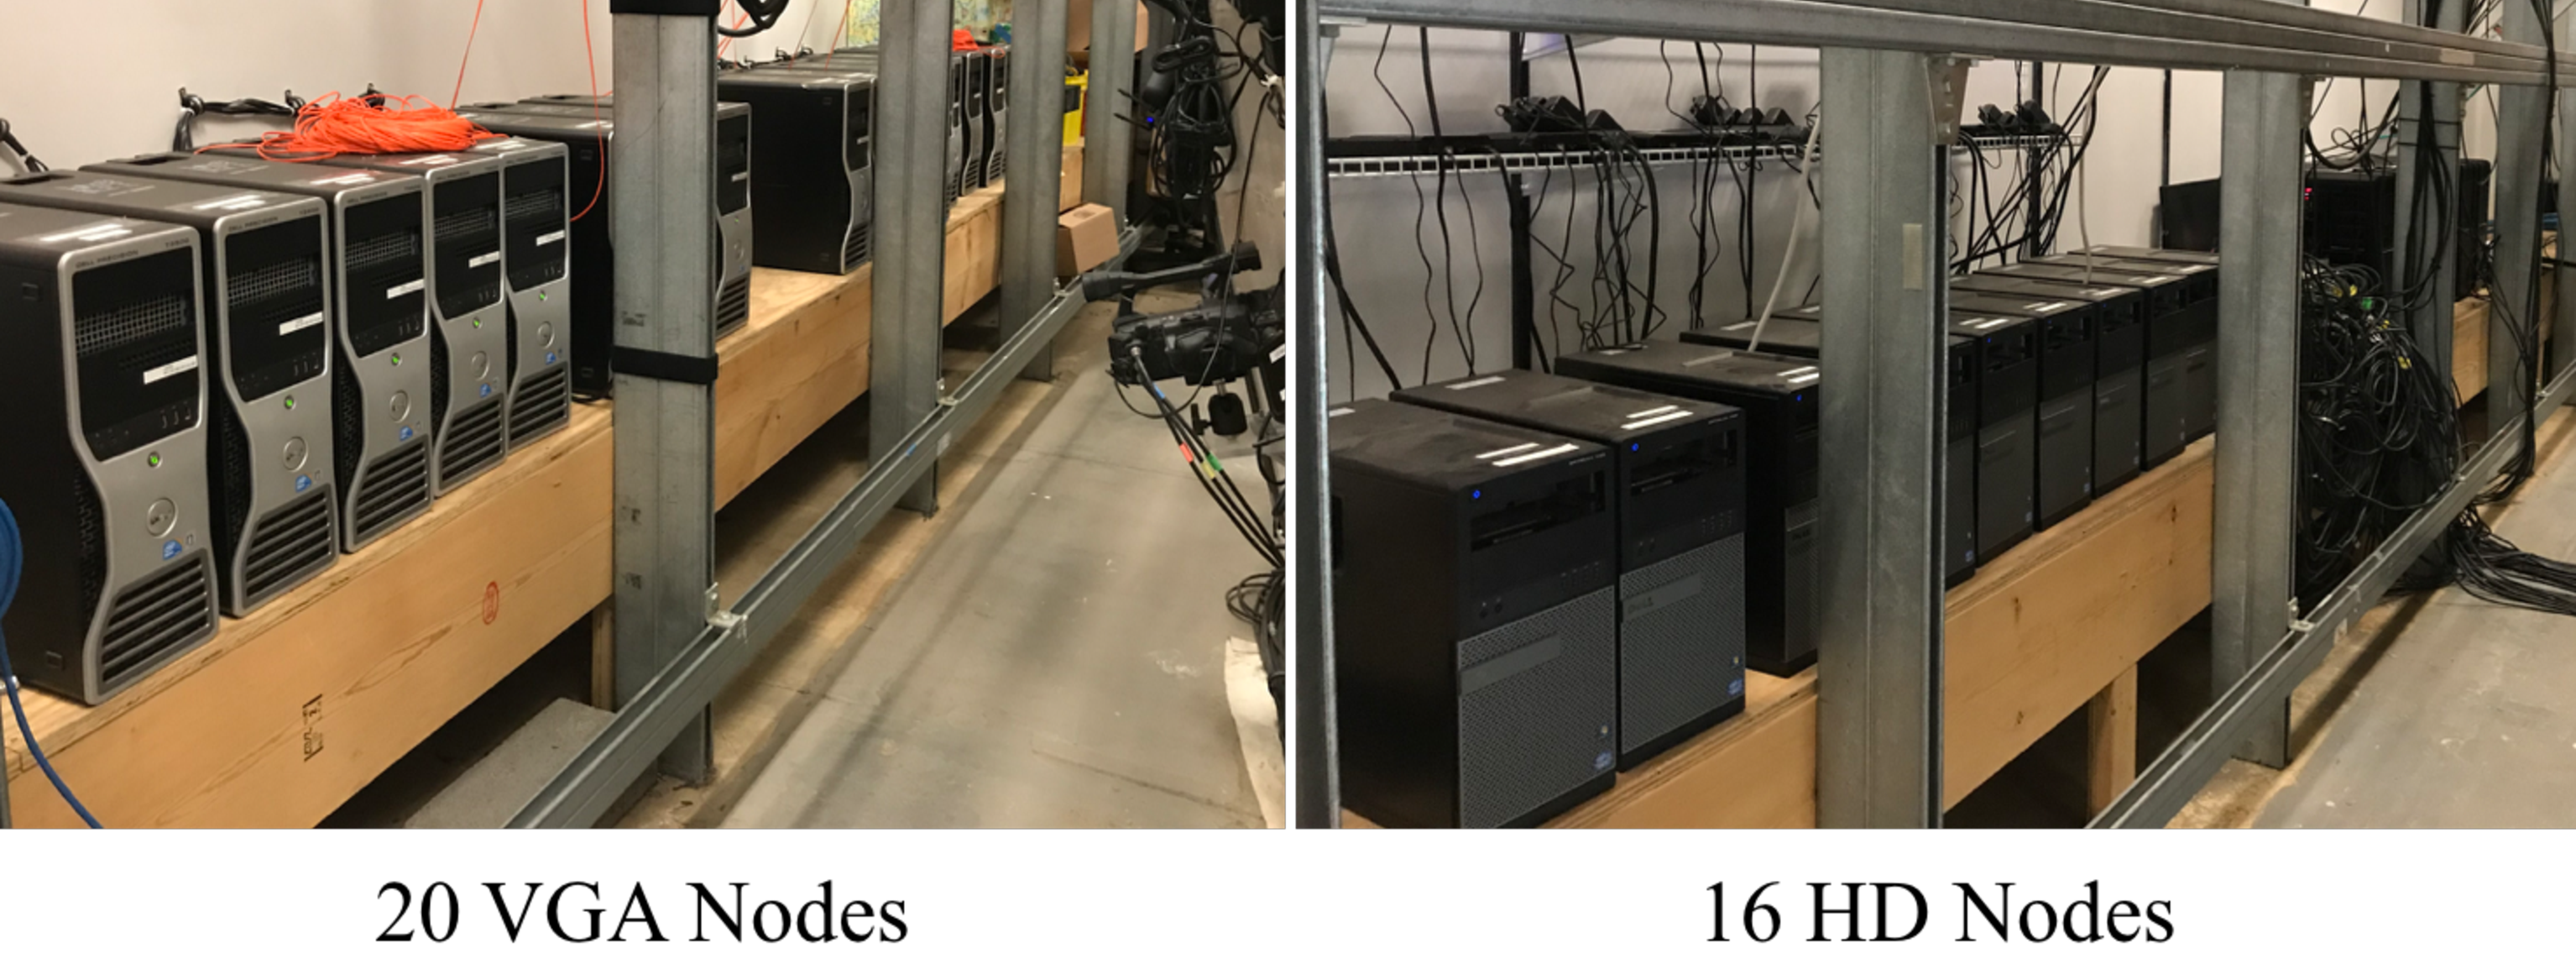
\includegraphics[trim=0 0 0 0,clip,width=\linewidth]{fig_system/machines}
	\caption{VGA subsystem is controlled by 20 node machines, and HD subsystem is controlled by 16 node machines. All nodes are connected and controlled by a master node to initiate the capture.}
	\label{fig:dome_machines}
\end{figure}
\begin{figure}[t]	
	\centering
	\begin{subfigure}{0.71\textwidth}
		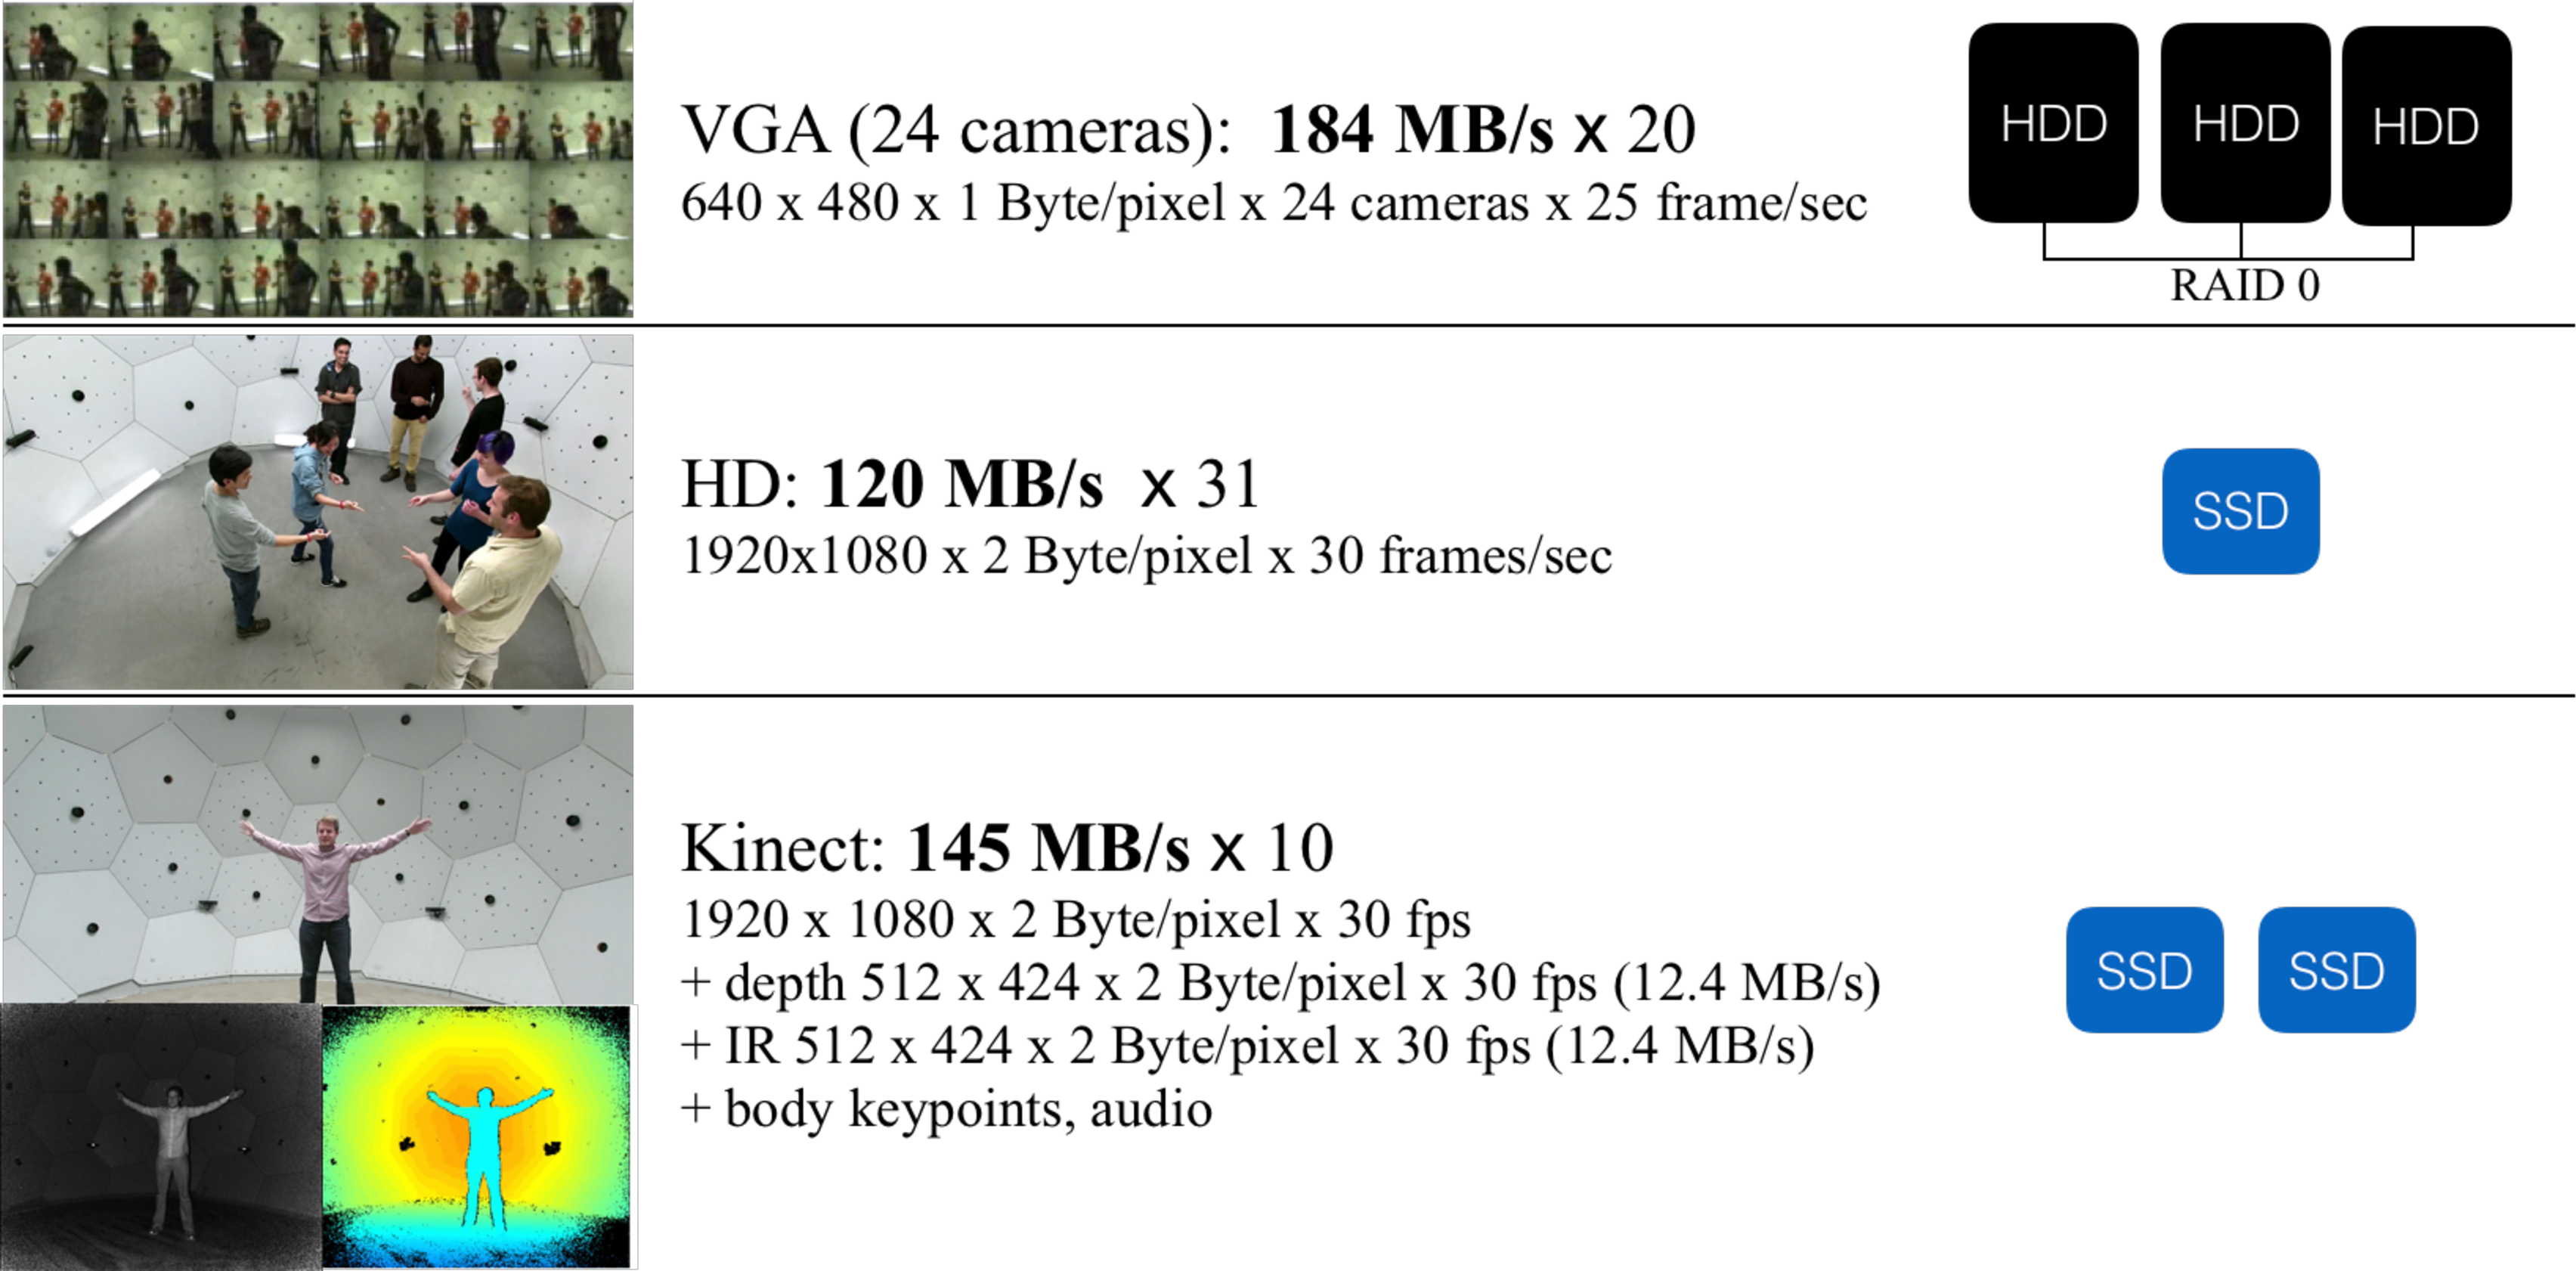
\includegraphics[width=\textwidth]{fig_system/storage}
		\caption{Data size and local storage for each node}
		\label{fig:dome_datasize}
	\end{subfigure}
	\begin{subfigure}{0.27\textwidth}
		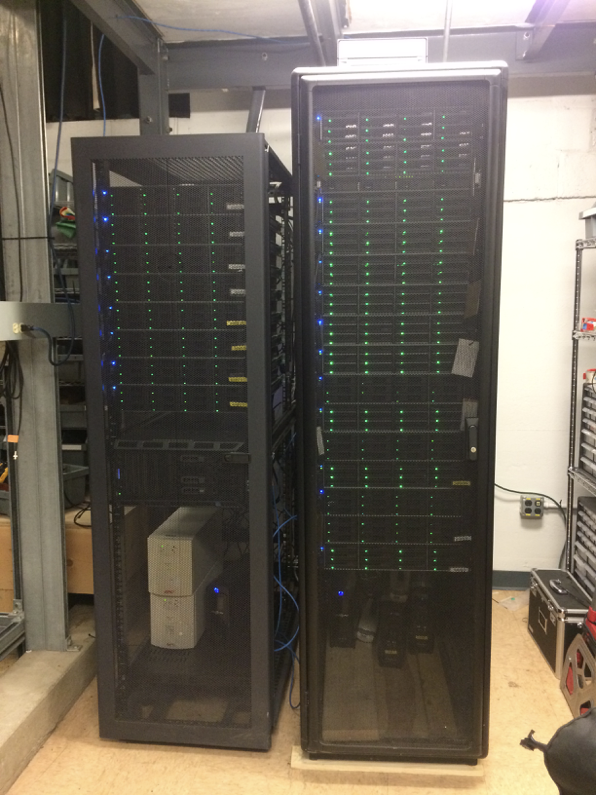
\includegraphics[width=\textwidth]{fig_system/dome_NAS}
		\caption{NAS sotrage system}
		\label{fig:dome_NAS}
	\end{subfigure}
	\caption{(a) Overall data size the Panoptic Studio generates per each second, and storage solutions for local nodes (b) Network Attached Storage (NAS) system to store the data for long-term.}
\end{figure}

\begin{figure}
	\centering       
	%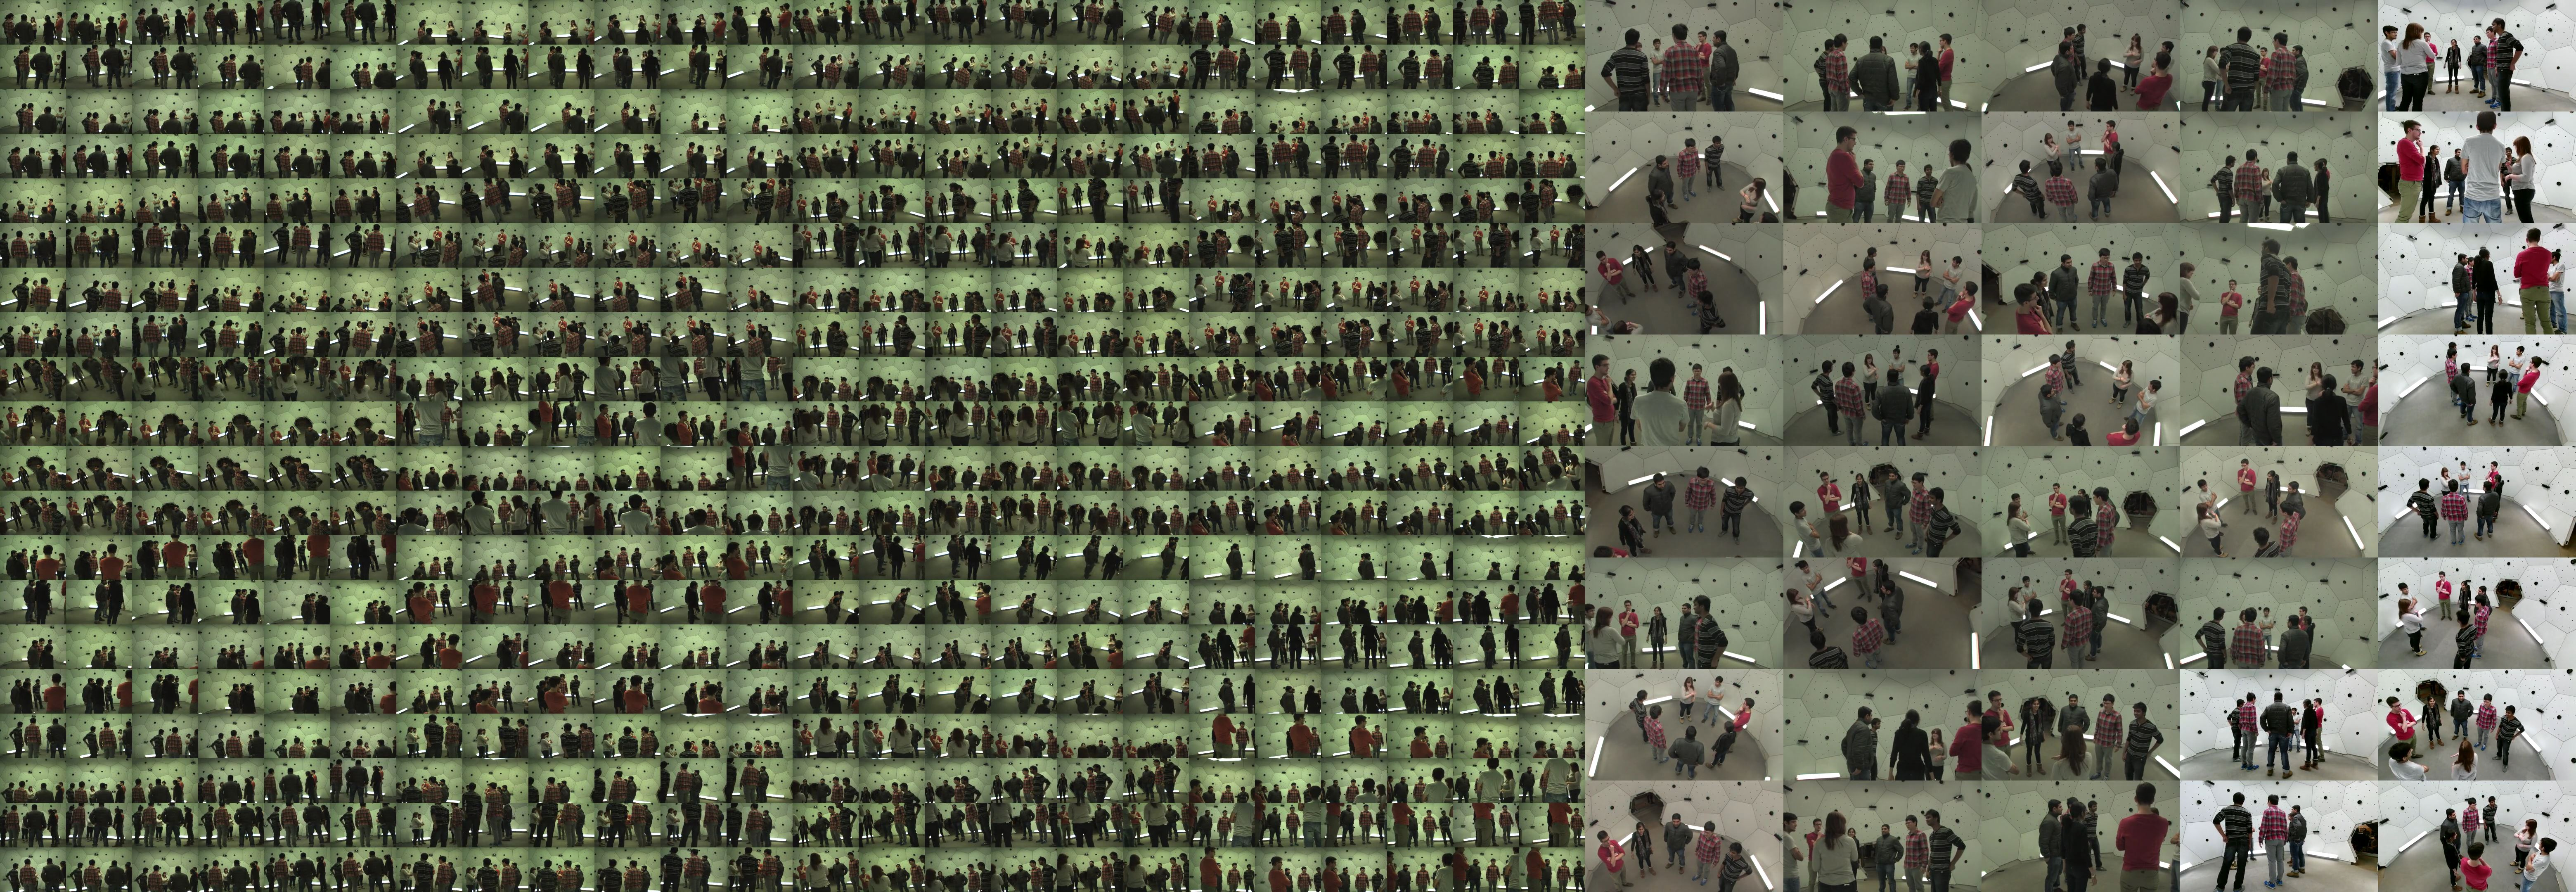
\includegraphics[trim=0 0 0 0,clip,width=\linewidth]{figures/Teaser}
	\includegraphics[trim=0 0 0 0,clip,width=\linewidth]{fig_system/480views_1126}
	\caption{An example scene from 520 camera views of the Panoptic Studio, from 480 VGA cameras, 30 HD cameras, and 10 RGB cameras of the RGB+D sensors.}
	\label{fig:dome_exampleScene}
\end{figure}

\begin{figure}
	\centering       
	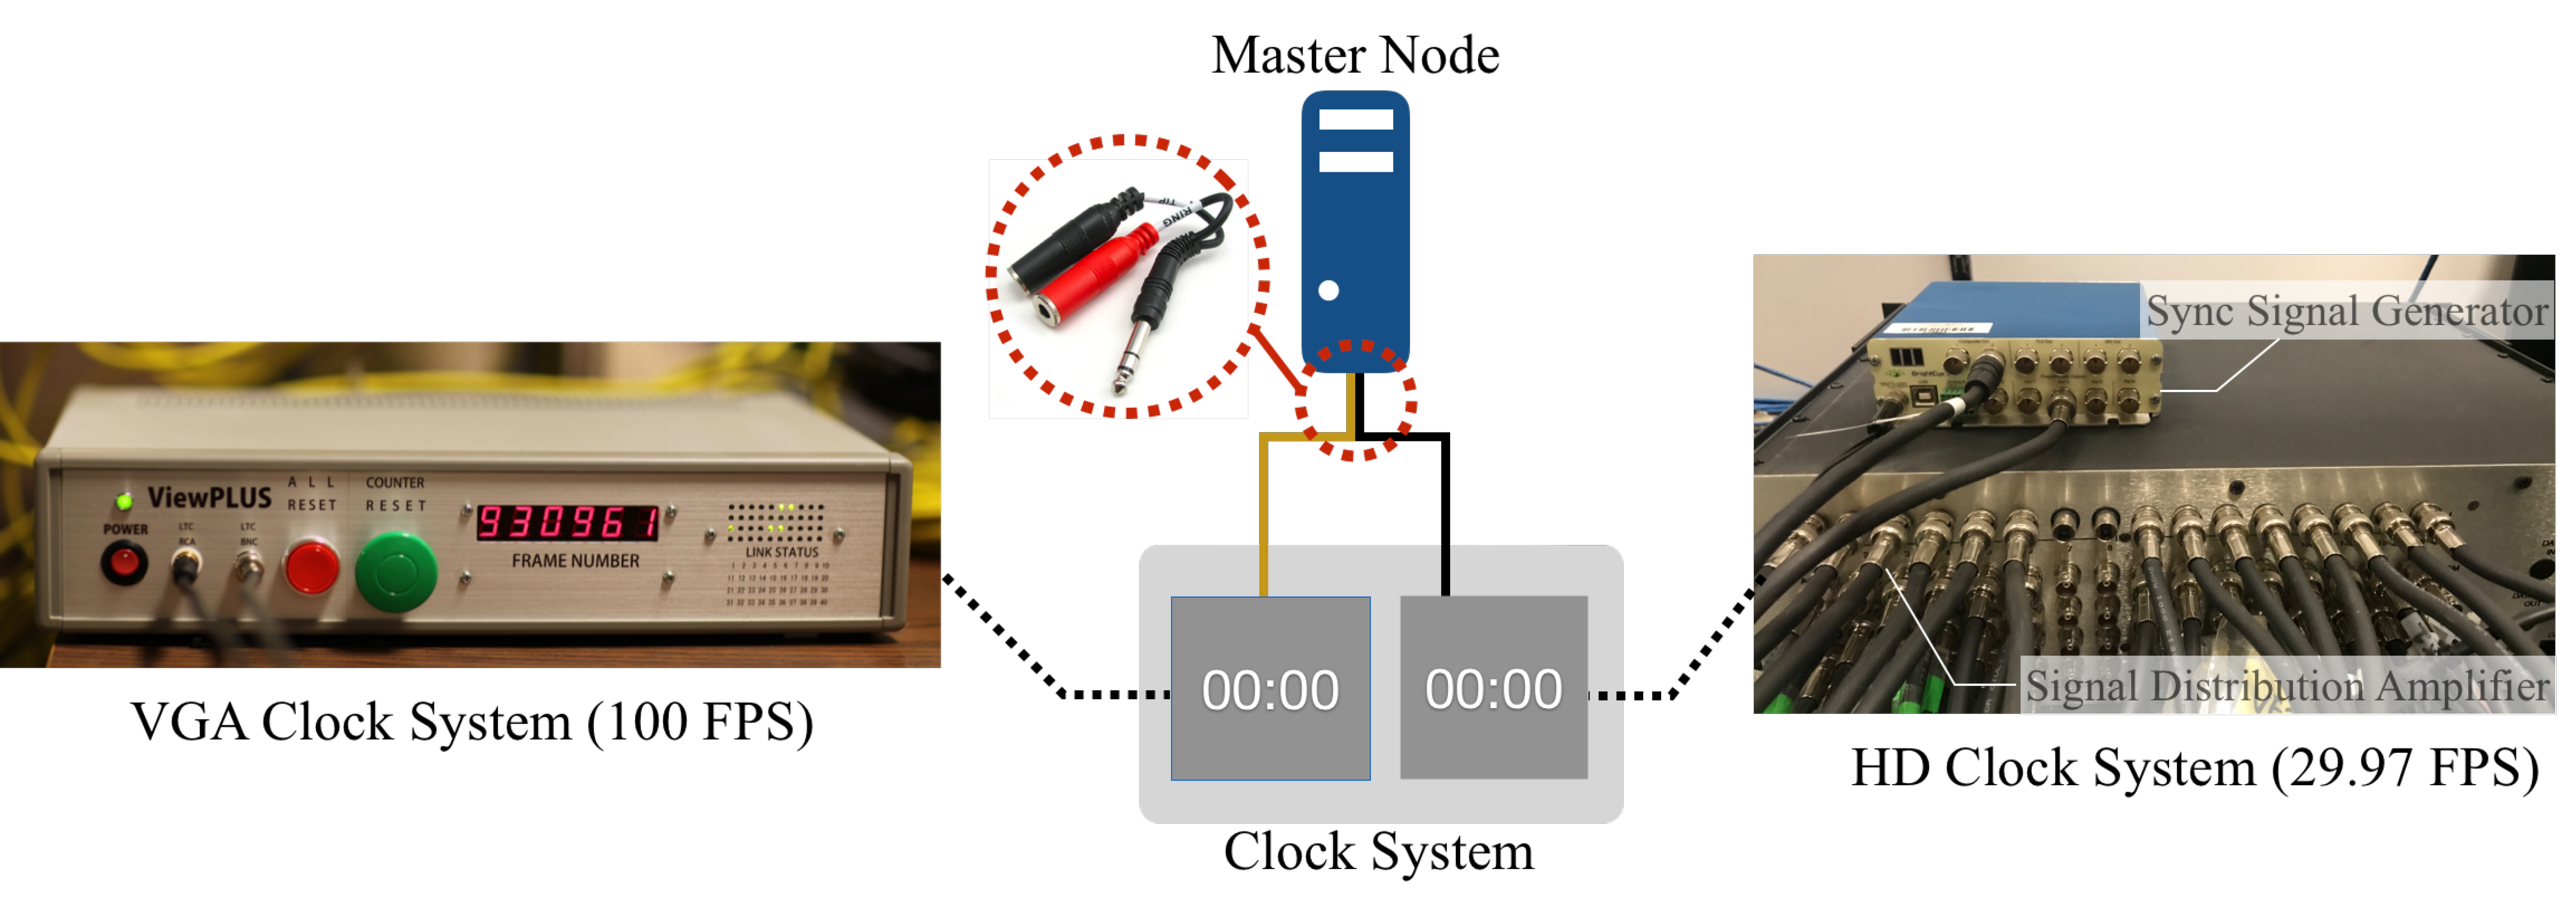
\includegraphics[trim=0 0 0 0,clip,width=\linewidth]{fig_system/dome_syncSystem}
	\caption{Time alignment between VGA camera system and HD camera system. The VGA clock generates 100 Hz time signals, which is downsampled to 25 Hz in VGA cameras, while the HD clock generates signals in 29.97 Hz. We connect them as a stereo audio signal and record it during the capture, which can be decoded afterward for temporal alignment.}
	\label{fig:dome_syncSystem}
\end{figure}
%The 31 HD cameras are installed at the center of each panel, and 
\noindent \textbf{HD Camera System:} HD cameras are also modularized and each pair of cameras are connected to a local node machine via SDI cables. We use Cannon XH G1s High Definition camcorders, which has 3 CCD sensors and capture scenes at 29.97 Hz with ($1920{\times}1080$) resolution. Each HD camera is equipped with a Canon 4.5-90 mm f1.6-f3.5 HD resolving lens, which we fit with a wide angle converter (Canon WD-H72). These cameras are genlocked and time-coded, driven by an external clock. The details of the HD camera modules are shown in Figure~\ref{fig:dome_hdSystem}. The data from a pair of HD cameras is transferred via HD-SDI to a local HD node. Each local node saves the data from two cameras to two SSD storage units respectively. 16 HD nodes are dedicated for 31 HD cameras, as shown in the right of the Figure~\ref{fig:dome_machines}.

%Additionally, a total of 10 Kinect v2 RGB+D sensors are mounted at heights of 1m and 2.6 meters, forming two rings with 5 evenly spaced sensors each. 

\noindent \textbf{RGB+D Sensor System:} Each RGB+D sensor is connected to a dedicated capture node that is mounted on the dome exterior. To capture at rates of approximately 30 Hz, the nodes are equipped with two SSD drives each and store color, depth, and infrared frames as well as body and face detections from the Kinect SDK. A separate master node controls and coordinates the 10 capture nodes via the local network. The details of this subsystem are described in the thesis work of Simon~\cite{simon2017}.


\noindent \textbf{Data Size and Storage System:} The data size of a minute of data from entire sensors is about 531 GB. The detailed data size for each sub-system is summarized in Figure~\ref{fig:dome_datasize} and an example scene captured by all the sensors are shown in the Figure~\ref{fig:dome_exampleScene}. The data from each sensor module is first saved to a local storage system for each connected node. We use different solutions, based on the data size generated by each sensor module. For VGA module with 25 cameras, we use 3 HDDs integrated as RAID-0. This solution provides fast writing speed with sufficient storage size to store more than two hours of data, while the system is unstable with frequent RAID system failures. For each HD camera, we dedicate a 1TB SSD, which can store more than 2 hours of data. And for Kinect module, we dedicate two 1TB SSDs. The all sensor data in the local storages are transferred to NAS for long-term storage, shown in Figure~\ref{fig:dome_NAS}. Panoptic Studio has about 1.5 PB storage space.


%\begin{figure}
%	\centering       
%	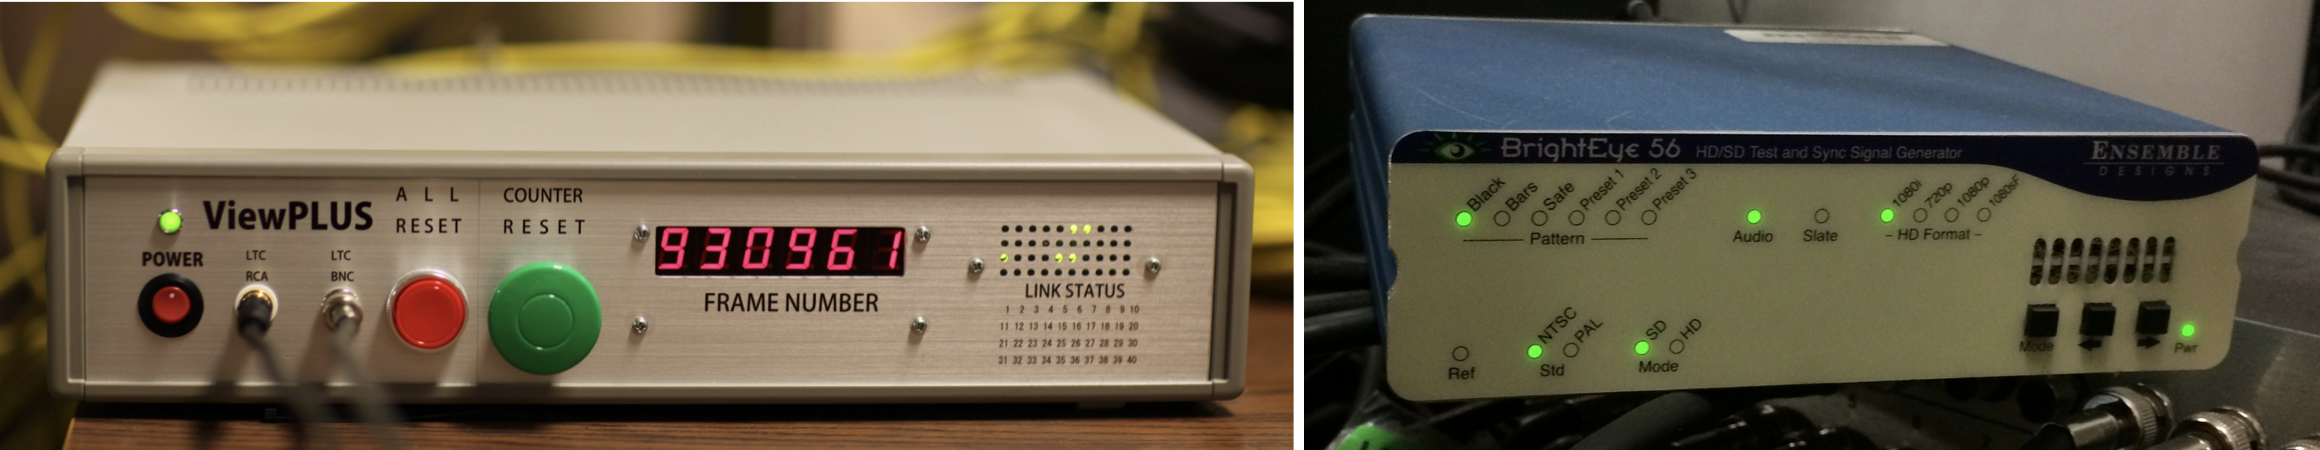
\includegraphics[trim=0 0 0 0,clip,width=\linewidth]{fig_system/dome_syncgens.png}
%	\caption{Sync generators.} 
%\end{figure}

\begin{figure}
	\centering
	%	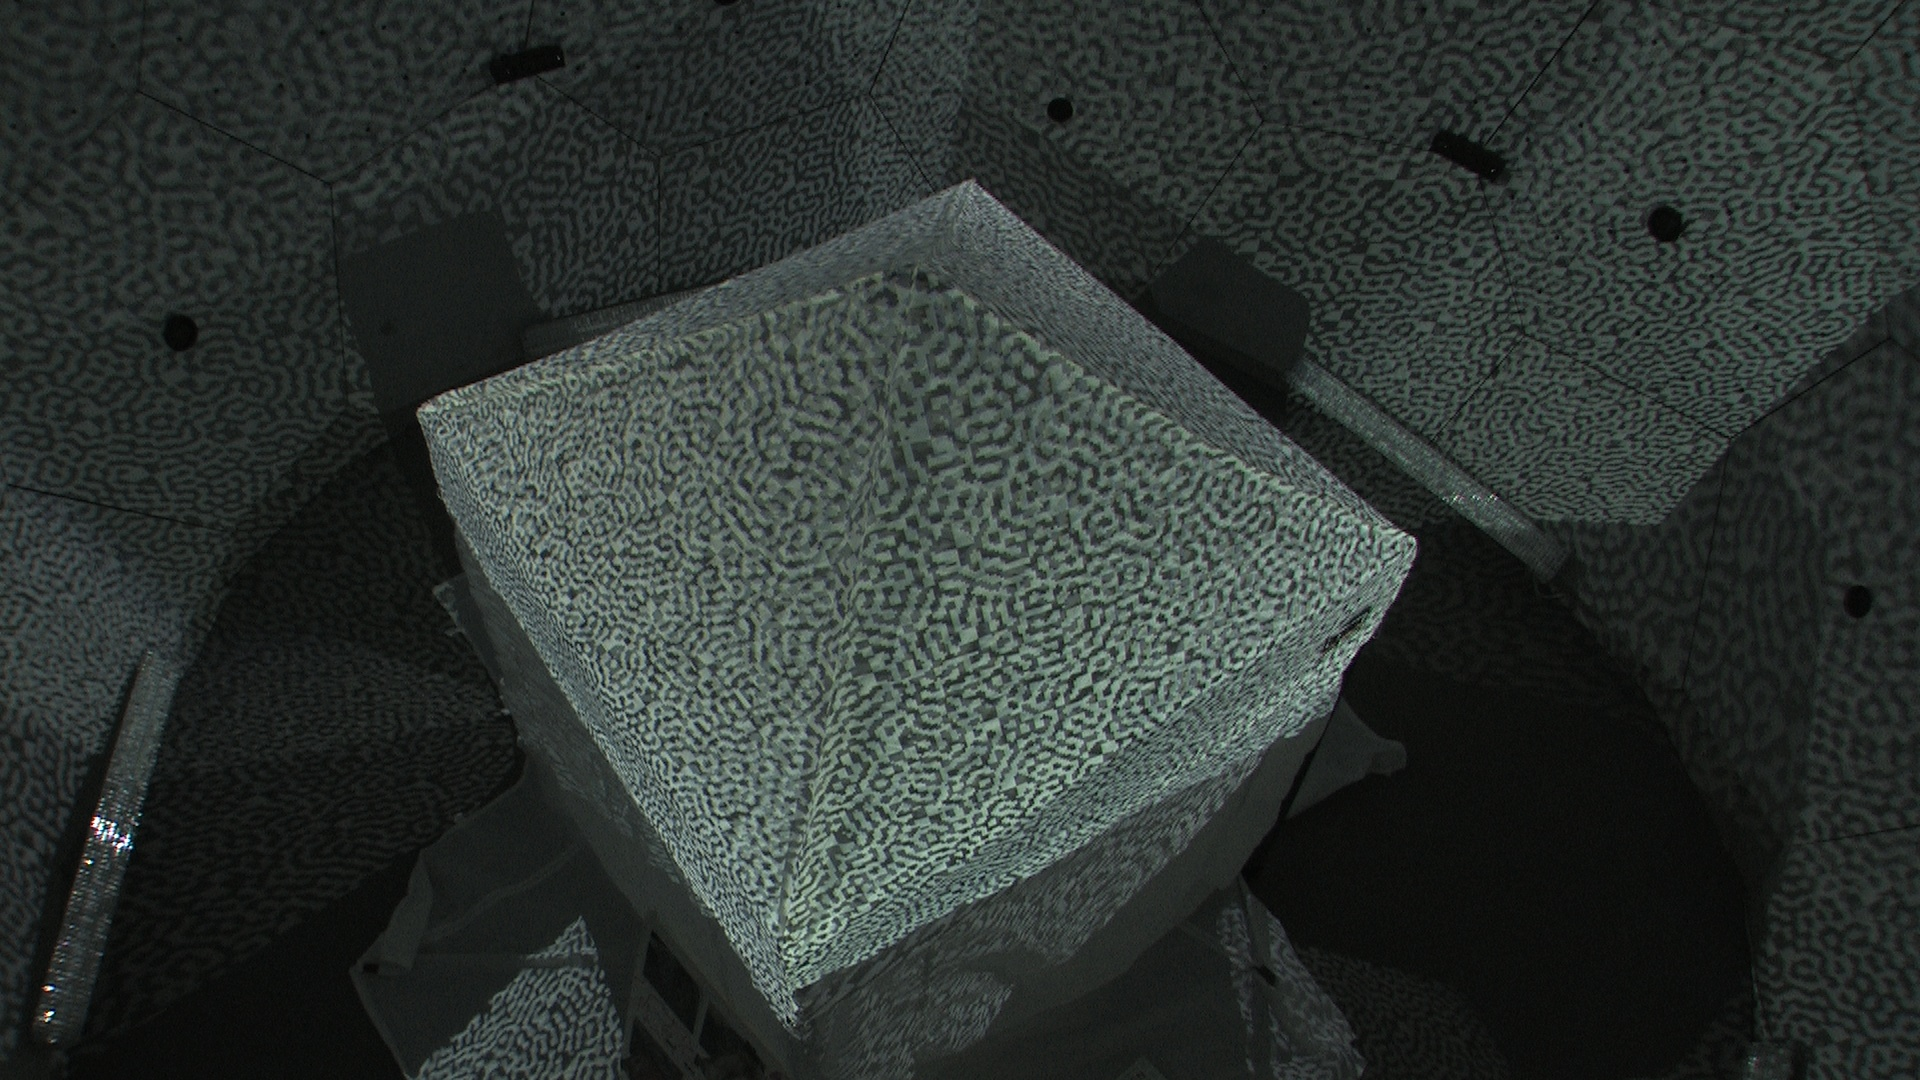
\includegraphics[height=0.2\linewidth]{figures/calib_tent_hd}
	%	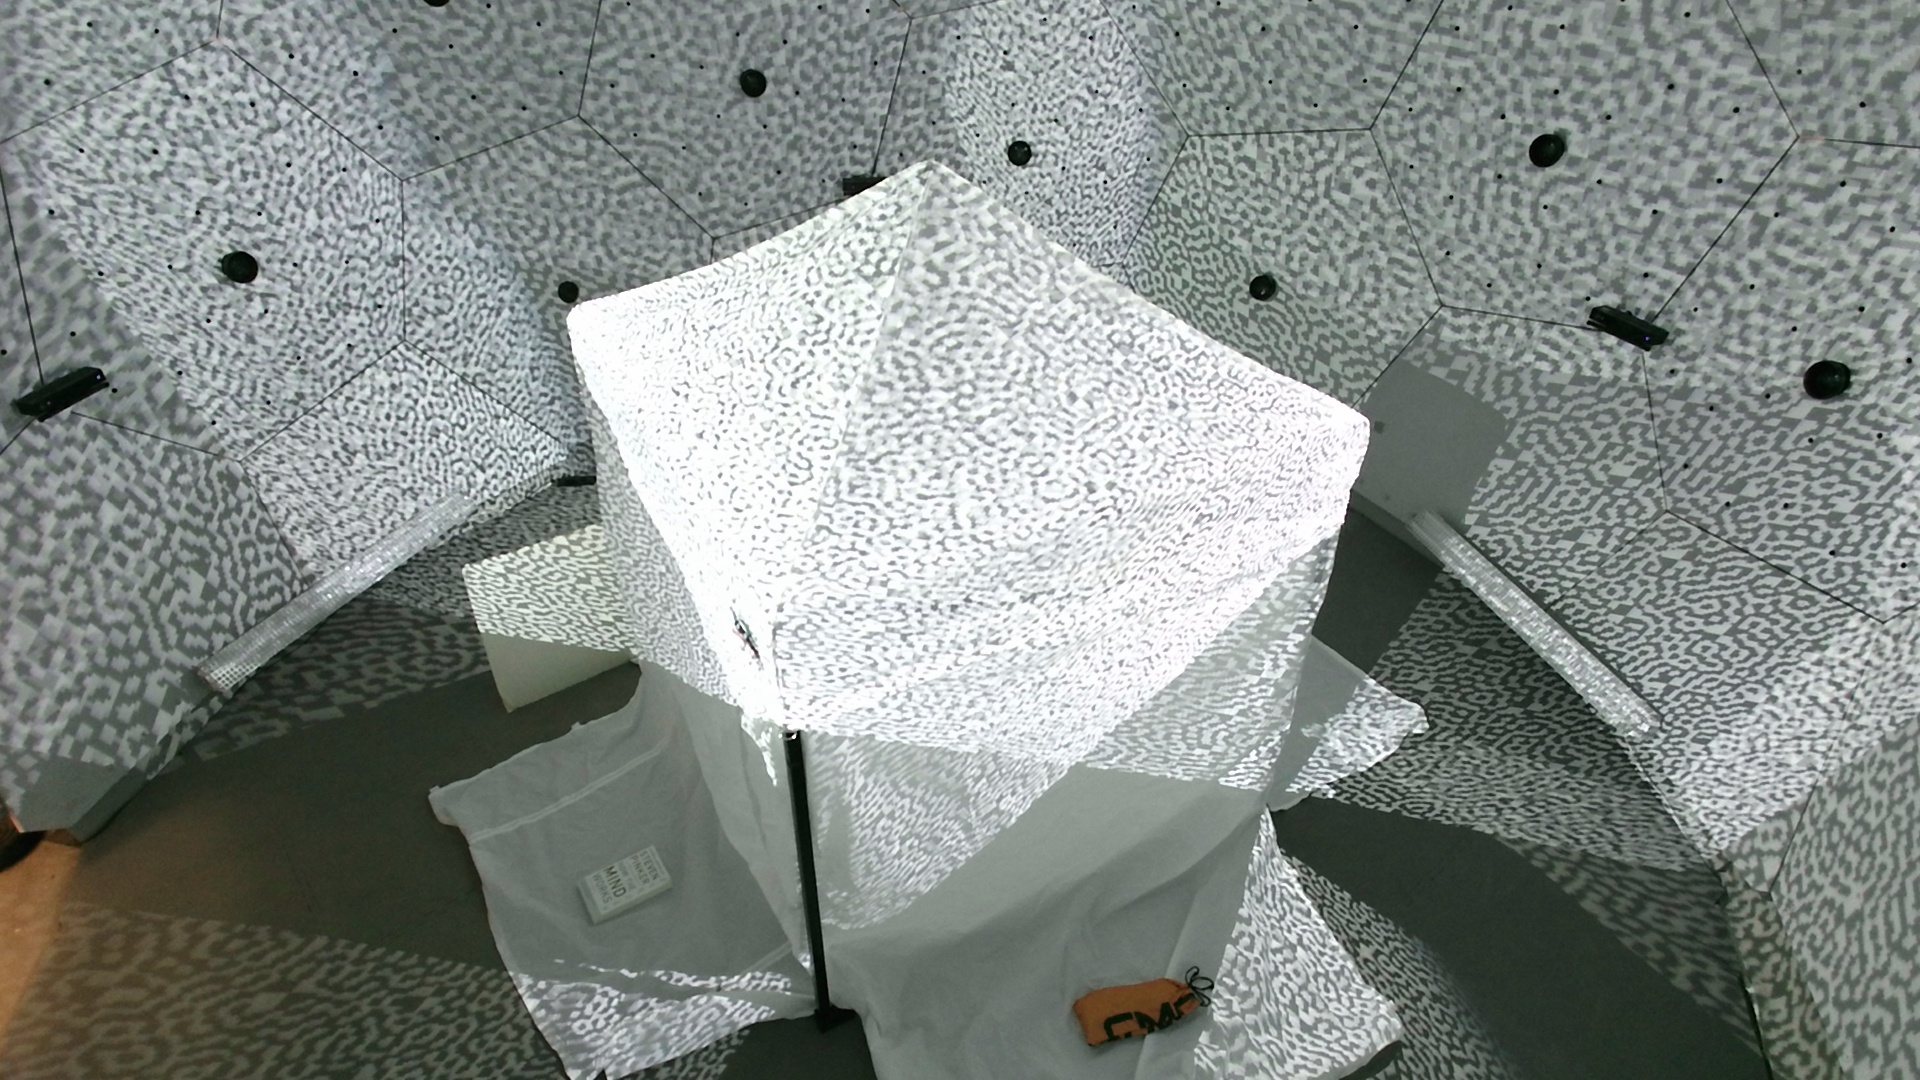
\includegraphics[height=0.2\linewidth]{figures/calib_tent_kinect}
	%	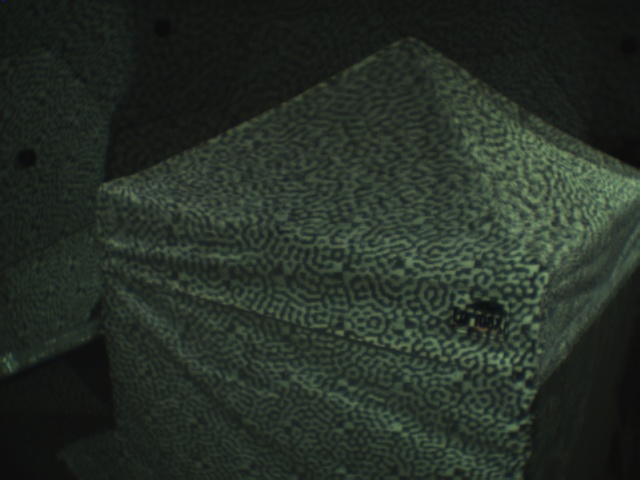
\includegraphics[height=0.2\linewidth]{figures/calib_tent_vga}\\
	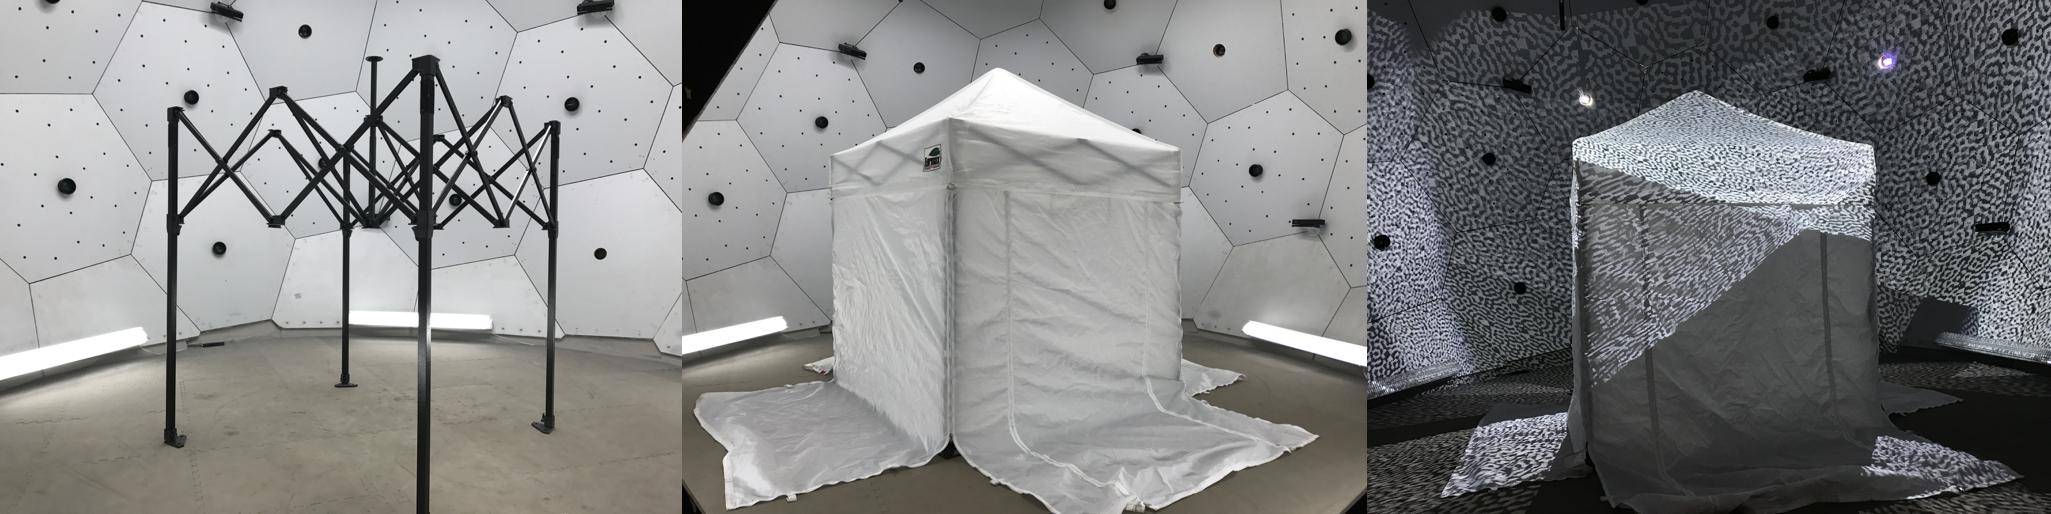
\includegraphics[width=\linewidth]{fig_system/cali_tent_3rdViews}\\
	\vspace{0.2cm}
	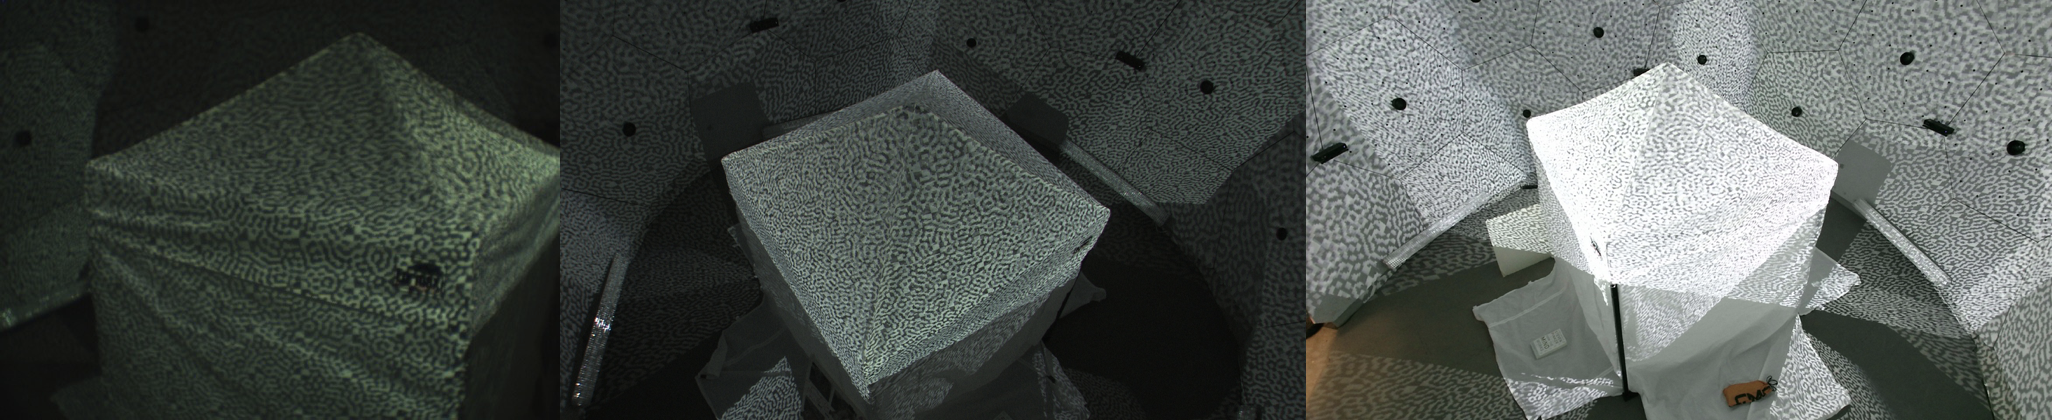
\includegraphics[width=\linewidth]{fig_system/cali_tent_camViews}\\
	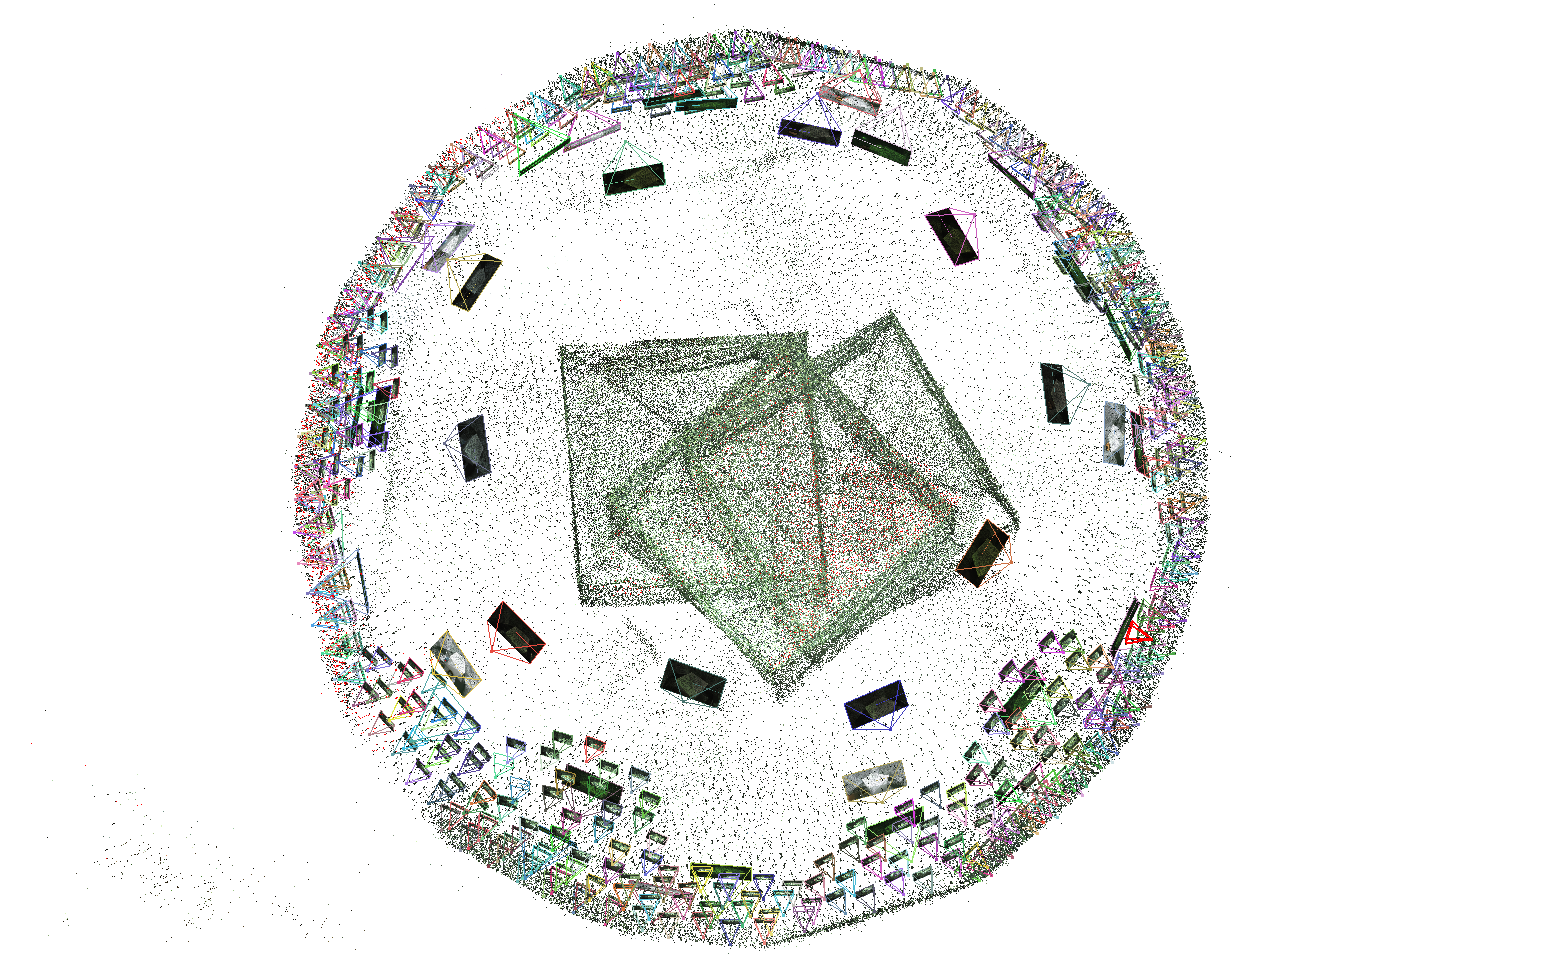
\includegraphics[trim=70 0 70 0,clip,width=0.45\columnwidth]{figures/domeCalib/38}  
	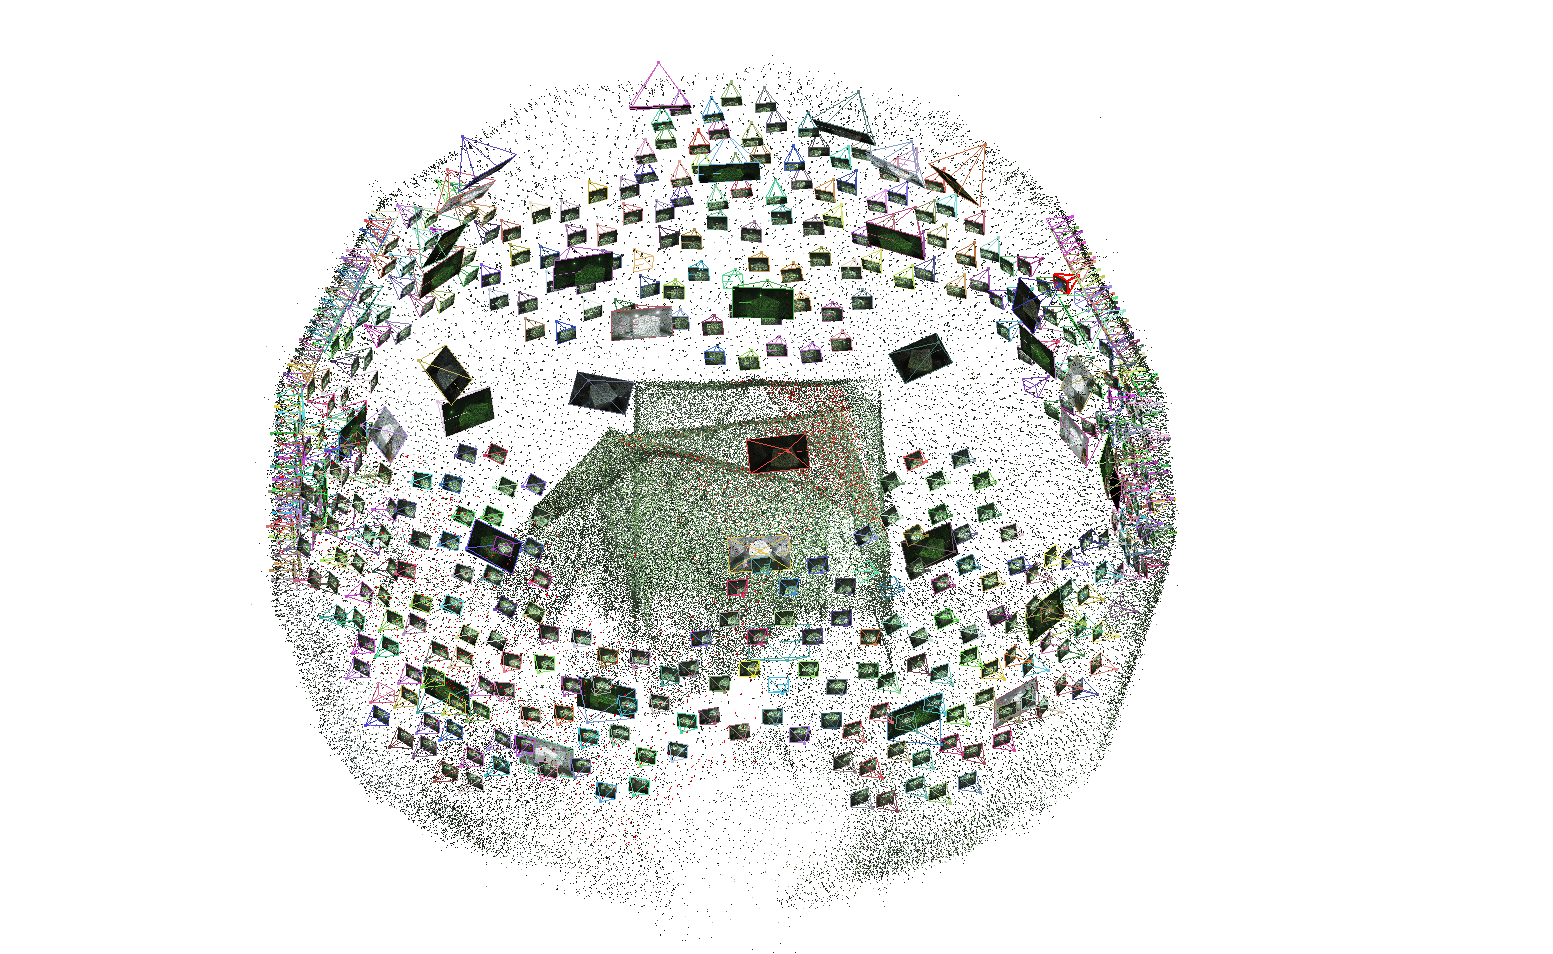
\includegraphics[trim=60 0 80 0,clip,width=0.45\columnwidth]{figures/domeCalib/39}  
	\caption{For efficient spatial calibration process, we use a portable folding tent structure by projecting random patterns from 5 DLP projectors. (Top row) the portable tent and projected patterns; (Middle left) a VGA view; (Middle center) an HD view; (Middle right) a Kinect view from its color camera; (Bottom row) Visualizations of 3D camera localization and a reconstructed 3D point cloud.} 
	\label{fig:spatialCalibration}
\end{figure}

\section{Temporal Calibration for Heterogeneous Sensors}
Synchronizing the cameras is necessary to use geometric constraints (such as triangulation) across multiple views. In our system, we use hardware clocks to trigger cameras at the same time. Because the frame rates of the VGA and HD cameras are different (25 fps and 29.97 fps respectively) we use two separate hardware clocks to achieve shutter-level synchronization among all VGA cameras, and independently among all HD cameras. To precisely align the two time references, we record the timecode signals generated from the two clocks as a single stereo audio signal, which we then decode to obtain a precise alignment at sub-millisecond accuracy, as shown in Figure~\ref{fig:dome_syncSystem}.

Time alignment with the Kinect v2 streams (RGB and depth) is achieved with a small hardware modification: each Kinect's microphone array is rewired to instead record an LTC timecode signal\footnote{As a result of this modification, microphone output on the Kinects is therefore discarded. More details about this hardware modification are available upon request.}.  This timecode signal is the same that is produced by the genlock and timecode generator used to synchronize the HD cameras, and is distributed to each Kinect via a distribution amplifier. We process the Kinect audio to decode the LTC timecode, yielding temporal alignment between the recorded Kinect data---which is timestamped by the capture API for accurate relative timing between color, depth, and audio frames---and the HD video frames. Empirically, we have confirmed the temporal alignment obtained by this method to be of at least millisecond accuracy.
%, with the RGB sensor being a rolling shutter with a scan time of approximately 25ms.


\section{Spatial Calibration}
We use Structure from Motion (SfM) to calibrate all of the 521 cameras. To easily generate feature points for SfM, five projectors are also installed on the geodesic dome. For calibration, they project a random pattern on a white structure as shown in the Figure~\ref{fig:spatialCalibration}, and multiple scenes (typically three) are captured by moving the structure within the dome. We perform SfM for each scene separately and perform a bundle adjustment by merging all the matches from each scene. We use the VisualSfM software~\cite{vsfm} with 1 distortion parameter to produce an initial estimate and a set of candidate correspondences, and subsequently run our own bundle adjustment implementation with 5 distortion parameters for the final refinement. The computation time is about 12 hours with 6 scenes (521 images for each) using a 6 core machine. 
In this calibration process, we only use the color cameras of Kinects. We additionally calibrate the transformation between the color and depth sensor for each Kinect with a standard checker board pattern, placing all cameras in alignment within a global coordinate frame.
%and the depth cameras are stitched to the global camera coordinate of other cameras in the end. 

\section{Lighting, Audio Recording, and Capture Softwares}

\noindent \textbf{Lighting:} We use a relatively low-cost solution for lighting by installing fluorescent lamps on the ceiling and floors, as shown in Figure~\ref{fig:dome_lighting}. The floor lights are important to reduce the shadow issues of the scenes. 

\noindent \textbf{Audio Recording:} Audio from microphones can be easily recorded and synchronized with cameras by connecting microphones to HD cameras. Each HD camera has two mono microphone inputs, by which the audio signals are saved as a stereo audio file. We installed one microphone on the floor and two microphones on the ceiling. We also use 20 wireless lapel microphones by connecting the wireless receivers to HD cameras, as shown in Figure~\ref{fig:dome_mic}. Each lapel microphone is assigned to a subject during the social interaction capture.  

\noindent \textbf{Capture Softwares:} As an important part of the system, we built several custom software systems to control the capture process. Each subsystem is controlled by a separate capture software which needs to be initiated to capture entire system together. We built a simple shell script to make this conveniently in the master node. For VGA, we built a server-client module, where a local server is opened and run at each VGA node to communicate with the master node. In the master node, users can check the status of each VGA module, visualize the camera views in real-time streaming, and initiate the capture. The VGA capture tool is shown in the Figure~\ref{fig:dome_vgaSW}. For the HD, we simply use a secure shell (SSH) protocol to automatically initiate the capture software at each machine. Kinect is separately controlled by the Kinect master node.

After the capture, the captured scenes from VGA and HD sensors can be visualized in our viewer, as shown in Figure~\ref{fig:dome_viewer}. The viewer loads capture data by remotely connecting all local storages. 

\begin{figure}
	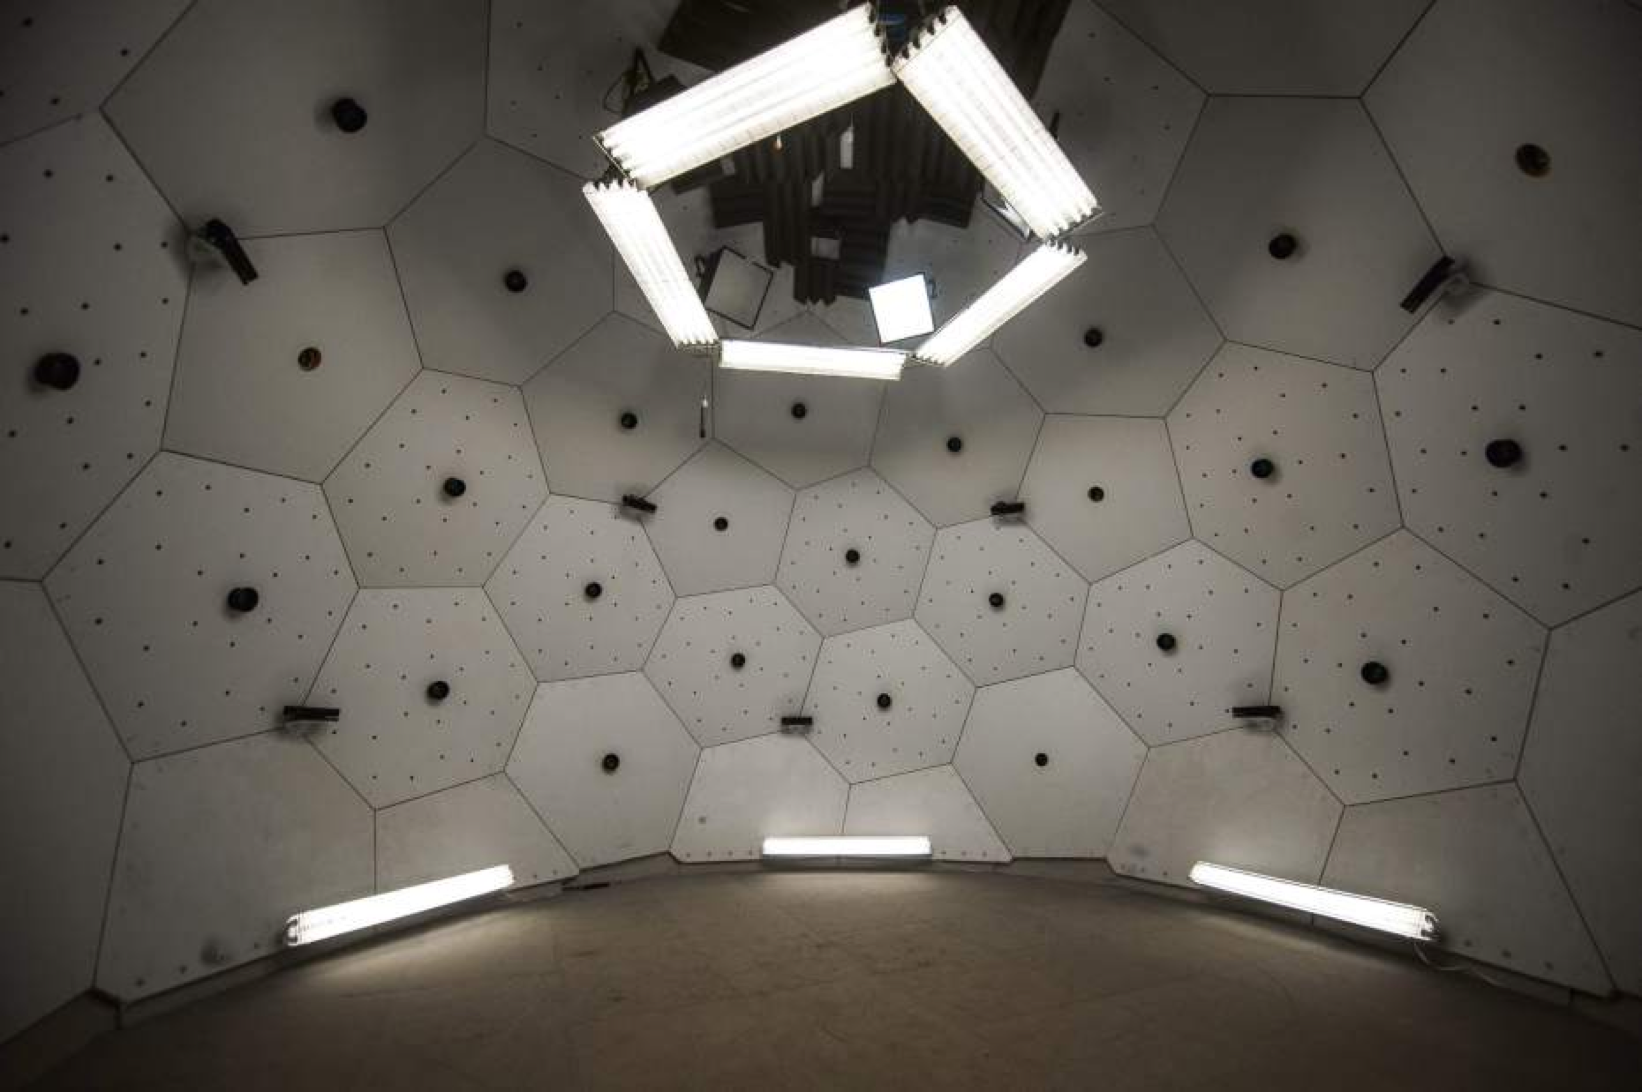
\includegraphics[width=\linewidth]{fig_system/dome_lighting}
	\caption{We use a relatively low-cost solution for lighting by installing fluorescent lamps on the ceiling and the floor.}
	\label{fig:dome_lighting}
\end{figure}

\begin{figure}
	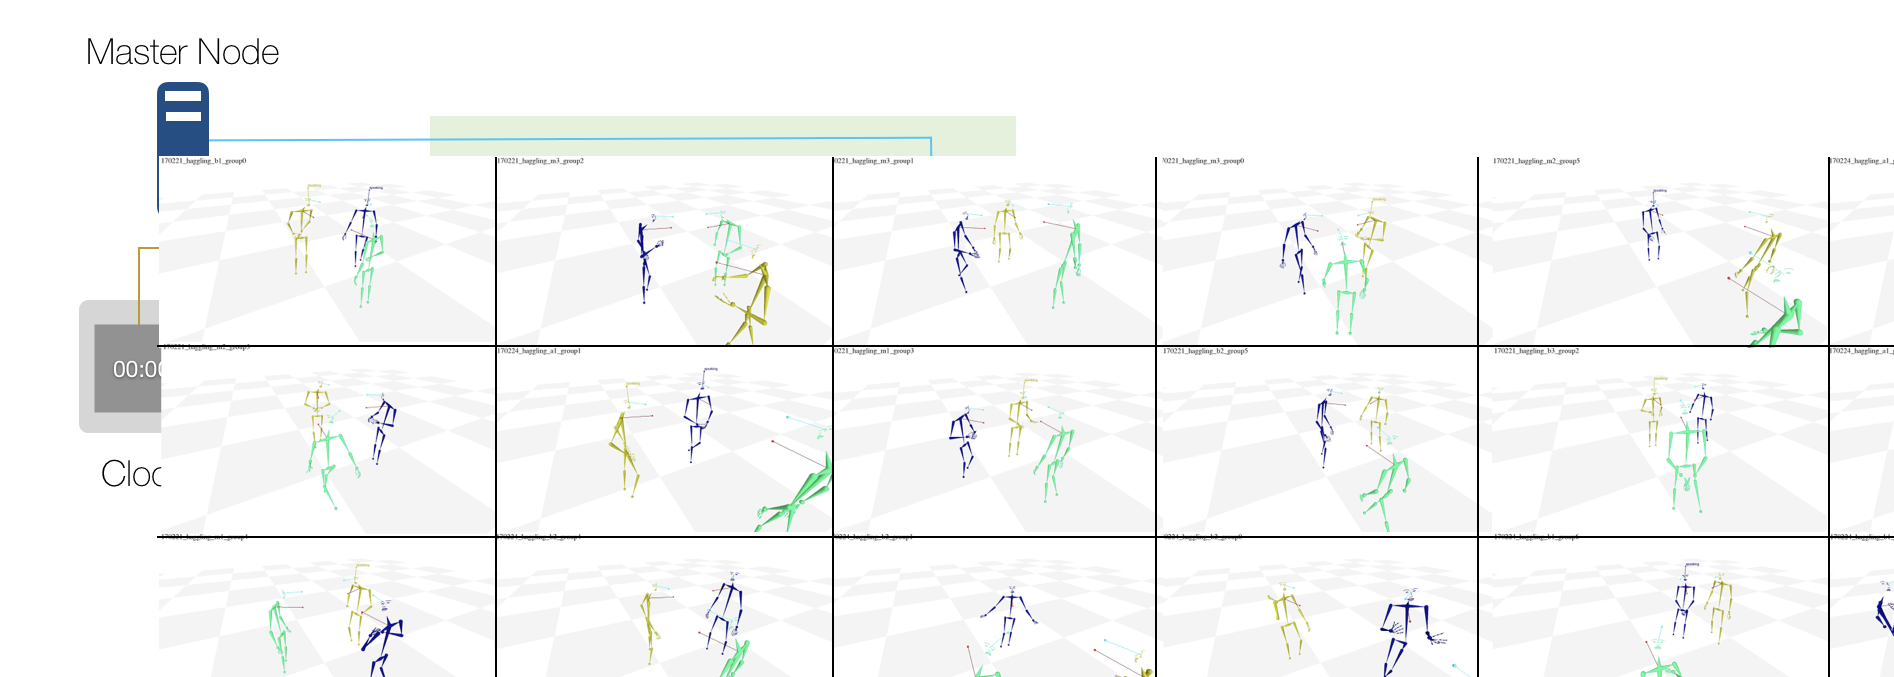
\includegraphics[width=\linewidth]{fig_system/dome_mic}
	\caption{Each HD camera has two mono microphone inputs, by which the audio signals are saved as a stereo audio file. We also use 20 wireless lapel microphones by connecting the wireless receivers to HD cameras.}
	\label{fig:dome_mic}
\end{figure}

\begin{figure}
	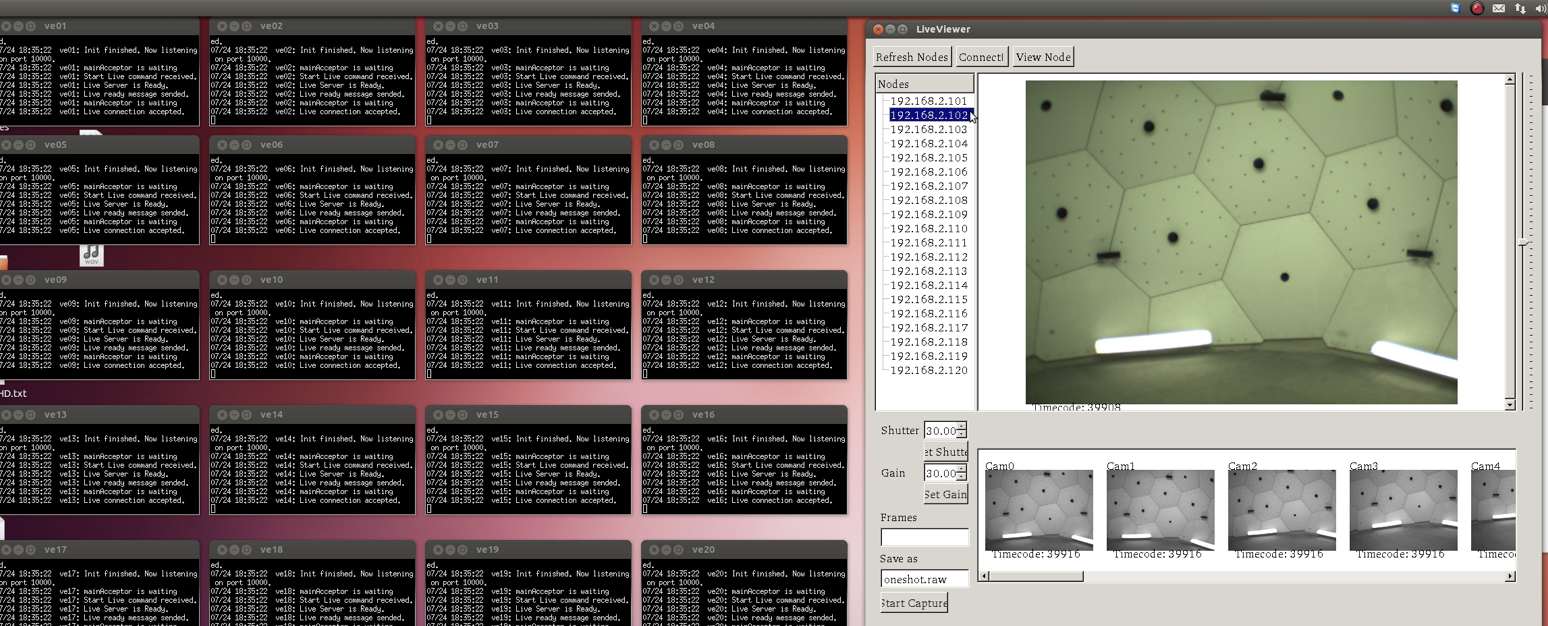
\includegraphics[width=\linewidth]{fig_system/dome_sw_capture.png}
	\caption{A capture software for VGA sub-system. In the master node, users can check the status of each VGA module (black consoles on the left), visualize the camera views in real-time streaming (the GUI tool on the right), and initiate the capture.}
	\label{fig:dome_vgaSW}
\end{figure}\vspace{0.5cm}
	
\begin{figure}[t]
	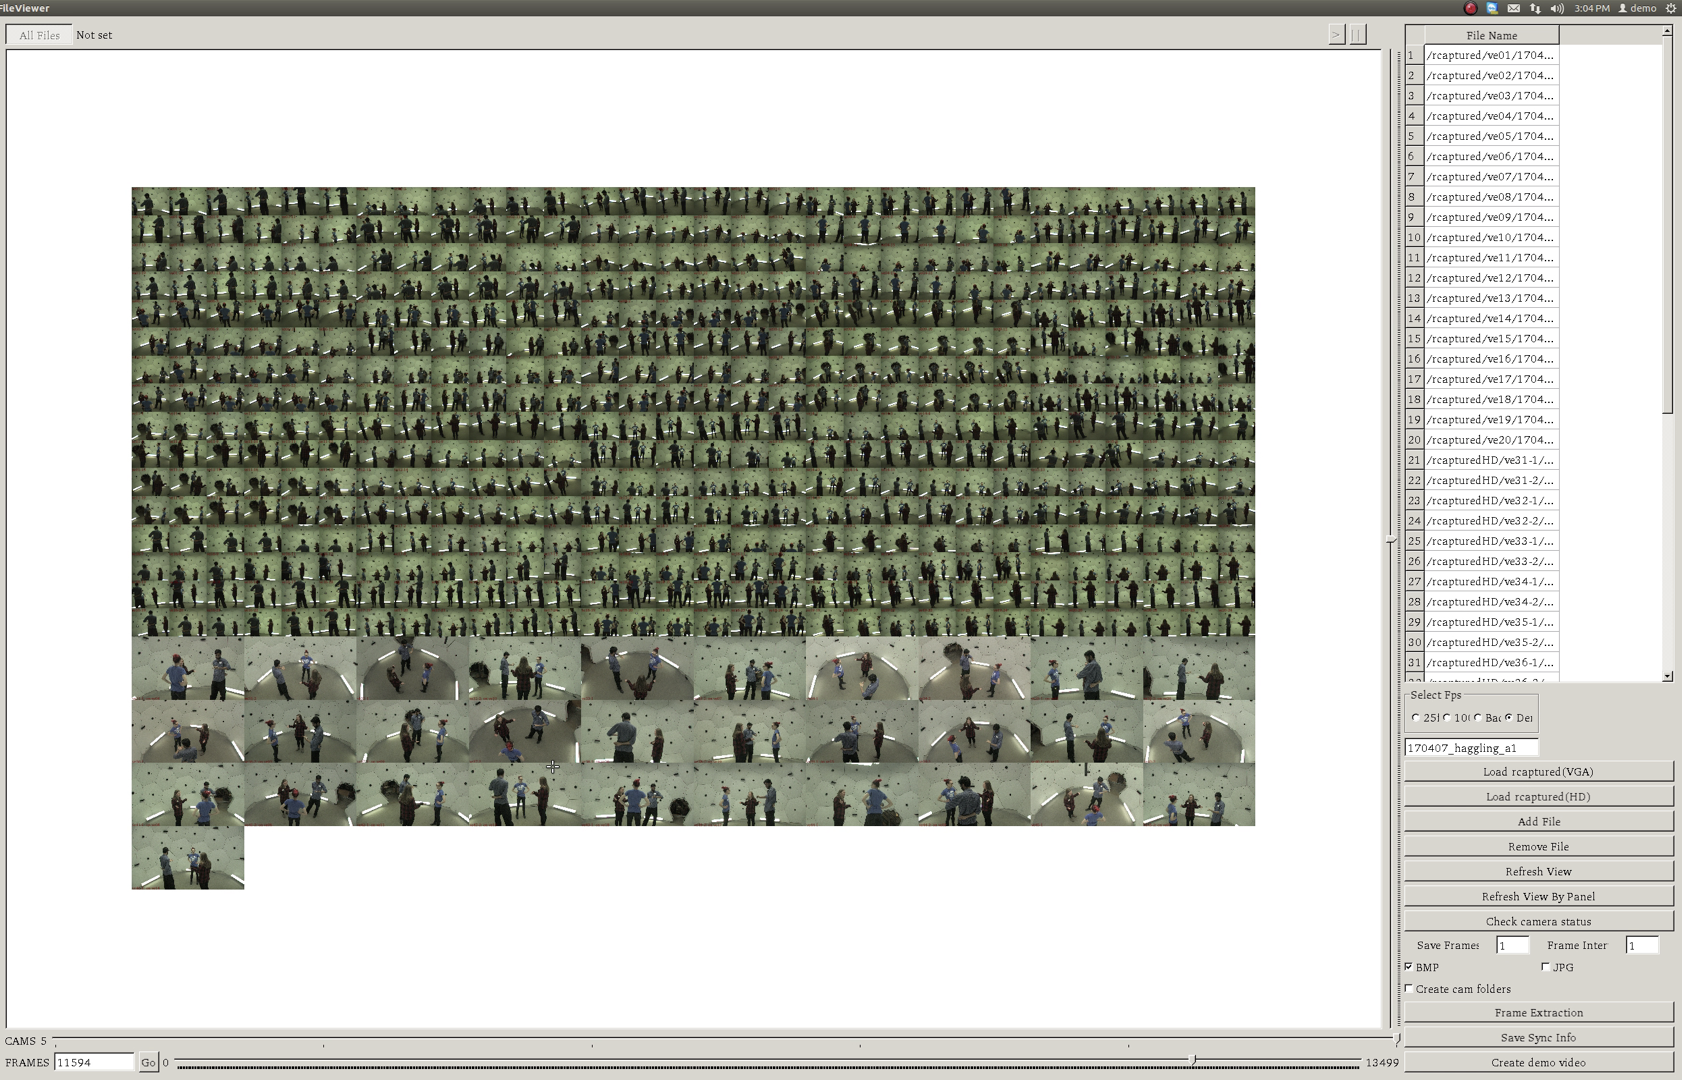
\includegraphics[width=\textwidth]{fig_system/dome_sw_viewer.png}
	\caption{A viewer to visualize the captured data from VGA and HD cameras.}
	\label{fig:dome_viewer}
	%\caption{Panoptic Studio Software System}
\end{figure}

\section{Limitations}
We found two limitations in our hardware design which can be reconsidered for follow-up research. The first is the incompatible frame rates among heterogeneous sensors, especially between HD cameras and VGA cameras, which makes it hard to fuse them for 3D reconstruction. Due to this reason, our method currently uses VGA cameras only, but we expect that this issue can be dealt with by interpolating cues in  the common time domain, because all the sensors are temporally aligned in millisecond level. The second issue is that all the camera views mainly focus on the center of the dome and, thus, fewer views are available at the edges of the capture volume. Such design is ideal given the assumption that subjects are located at the center of the system, but we observe that sometimes people tend to stand near the walls during social interactions. An alternative direction would be to make cameras focus on random locations so that view coverage can be uniformly spread throughout the working volume. 

%\section{Lighting}
%\section{Storage}
%\section{Hardware Details}
%\section{Capture Procedures}
%\section{Data Size}

%We use projectors to generate patterns. 
%We turn on projector one by one to reduce interference among them. 
%We run SfM using all the data. 
%We merge all the matching into a whole optimization. 
%
%With/Without tent
%All projectors/each projectors
%1 tent location, several tent location
%
%We evaluate the accuracy using a single scene with 2D maching points. Using each calibration, we reconstruct 3D and compute reprojection  error. 
%We use leave-out method to check each camera's reprojection error. 
%For kinect, we use checker board pattern. 
%Temporal alignment
%Among VGA
%Among HD
%Among Kinect
%VGA-HD
%VGA-HD-Kinect




\pagebreak
%	
%%	\part{Measuring Social Signals}
	\part{Reconstructing Social Signals}
	\epigraph{``Measure what is measurable, and make measurable what is not so."\par\raggedleft--- \textup{Galileo Galilei}}
	
%	Scientific achievements are often preceded by new innovations of measurement methods. Similarly, a method to accurately measure social signals at high resolution is the key to computationally analyze nonverbal communications. In this part of thesis, we build a system, the Panoptic studio, developed to capture social interactions, and present novel algorithms to measure full body motion of multiple people in social situations. The measured social signals include 3D movements of anatomical landmarks from face, body, and hands, and also contain dense 3D trajectories from body surfaces with part labels. Our method also enables to build a deformable 3D human model to capture dense 3D mesh structures for human body motion. 
%	\pagebreak
%	
	<<<<<<< HEAD:Chapter3/method_trajectorystream.tex
% !TEX encoding = UTF-8 Unicode
% !TEX root = ../thesis.tex

\chapter{Measuring Dynamic Dense 3D Surface Movements}
\label{chapter:trajectory}

Important messages during communication are often transmitted by subtle body movements. Accurately measuring such body movements in 3D across time is therefore important in analyzing social interactions. In this chapter, we aim at reconstructing dense 3D trajectories of dynamic 3D object, which we refer to as a \emph{3D trajectory stream}. However, such video-based 3D motion reconstruction is challenging, as natural motion produces a greater occurrence of measurement loss due to occlusion and also causes artifacts in imagery (e.g., motion blur and texture deformation). Utilizing a large number of cameras can address these challenges, because it is likely to (1) narrow the average baseline between nearby cameras, (2) reduce the occurrence of occlusion, and (3) provide robustness to measurement noise due to the surplus views. However, previous approaches are unable to fully leverage the increasing number of views to improve 3D tracking performance (in terms of the average length of reconstructed trajectories, the density of the trajectories, and the accuracy of localization). The principal cause of failure emerges from errors in reasoning about the time-varying \emph{visibility} of dynamic 3D points. Poor visibility reasoning severely affects tracking performance, as an algorithm cannot benefit from an alternate viewpoint if it is unaware that the point is visible in the alternate view. Furthermore, an erroneous conclusion that a point is visible in a camera can bias the reconstruction, often producing a characteristic ``jump" artifact where a point assumes the identity of a different location.


%Thousands of images exist for most significant landmarks around the world. The availability of such imagery has facilitated the development of large-scale 3D reconstruction algorithms, which fully leverage the number of views to produce dense and accurate 3D point clouds~\cite{Snavely:2006,Frahm:2010,Furukawa:2010}. Increasingly, landmark \emph{events} are also being captured at scale by hundreds of cameras at major sports games, concerts, and political rallies. However, analogous large-scale reconstruction algorithms, that are able to fully leverage a large number of views of an event to produce long, dense, and accurate 3D trajectories, do not yet exist. %In this paper, we present a method for reasoning about the visibility of the target points at each camera view, to reconstruct the 3D motion of a dynamic scene from a large number of views.



%Existing approaches have addressed these challenges through structural regularization, either by assuming a fixed topology \cite{Furukawa2008, Beeler2011} or by spatially regularizing the trajectories \cite{Basha2012a,Huguet2007,Vogel2011}. However, the performance of such approaches are usually limited in terms of accuracy and density of the reconstructed motion trajectories, due to the and they are failed in producing practically applicable 3D motion due to the limitation of measurement and over-regularization available information. 
%have been proposed usually in a limited system setup with relatively small number of cameras, as shown in Table~\ref{Table:camSettup}. 

%Following static reconstruction algorithms, existing approaches reason about visibility (if at all) assuming photometric consistency among cameras where the target point is visible \cite{Carceroni2002,Devernay2006,Furukawa2008}: if the local appearance of a point matches the expected appearance, it is considered visible in that camera. However, photometric consistency tends to require frontal facing cameras (with respect to the tangent plane at the point), are susceptible to imaging artifacts, and require accurate estimates of the tangent plane normal at the point. Poor visibility reasoning severely affects tracking performance and obstructs the full benefit of a large number of unique viewpoints. 

In this chapter, we demonstrate a method that precise inference of point visibility allows reconstruction algorithms to fully leverage large numbers of views to produce longer 3D trajectories with higher accuracy. In particular, our core algorithmic contributions in this chapter are: (1) the use of motion consistency as a cue for the visibility of moving points; (2) the use of viewpoint regularity as a prior and a measure for viewpoint proximity; and (3) a maximum a posteriori (MAP) estimate for visibility estimation by probabilistically incorporating these cues with photometric and geometric consistency. We report empirical performance in reconstructing 3D motion captured by 480 VGA cameras\footnote{This research was conducted before we build the HD and RGB+D sensors in the Panoptic Studio} in scenes that contains significant occlusion, large displacement, and changes in the topology of the scene.

\begin{figure}[t]
	\begin{center}
		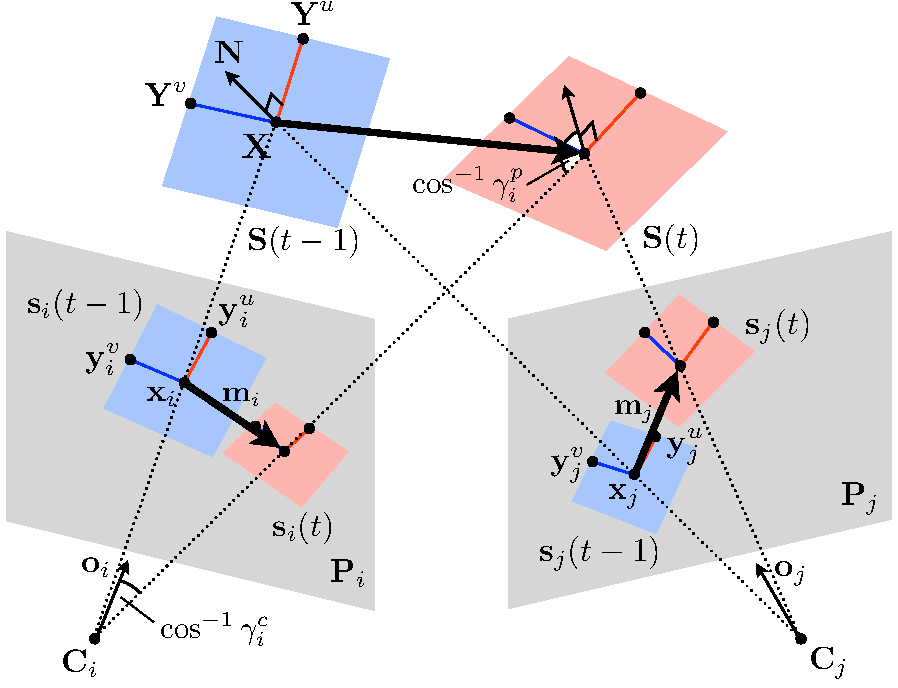
\includegraphics[width=0.6\linewidth]{figures/Notation_final}
		\caption{The motion of a patch between time $t-1$ and $t$ is reconstructed from multiple cameras.}
		\label{fig:notation}
	\end{center}
\end{figure}
%\interfootnotelinepenalty=10000
%\vspace{-0.2cm}
\section{Notation}
%\vspace{-0.2cm}
Our algorithm takes, as input, image sequences from $N$ calibrated and synchronized cameras over $F$ frames and produces, as output, 3D trajectories of $P$ moving points with their instantaneous orientations and associated visibility in each camera frame. Since the method is applied to each point independently, we consider only a single point here to simplify the exposition.

As shown in Figure~\ref{fig:notation}, we track a parallelogram patch centered on a target 3D point $\mathbf{X} \in \mathds{R}^3$, whose extent is defined by two additional points $\mathbf{Y}^u$ and $\mathbf{Y}^v \in \mathds{R}^3$. The texture information $\mathbf{Q} \in \mathds{R}^m$ associated with the patch is defined by a unit vector concatenating normalized intensity values at a fixed number of grid positions on the patch, where $m$ is the number positions in the grid\footnote{The texture vector $\mathbf{\mathbf{Q}}$ is normalized as follows:
	\begin{eqnarray}
	\mathbf{Q} = \frac{1}{\sqrt{\sum_{j=1}^m (Q_j-\overline{Q})^2}} \left[\begin{array}{c}Q_1-\overline{Q}\\\vdots\\ Q_m-\overline{Q} \end{array}\right] \label{Eq:normalized_texture}
	\end{eqnarray}
	where $\overline{Q} = \sum_{j=1}^m Q_j / m$ and $Q_j$ is the $j^{\textrm th}$ intensity value of the texture.}. 

The patch $\mathbf{S}(t)$ is denoted by the set $\{\mathbf{X}(t), \mathbf{Y}^u(t), \mathbf{Y}^v(t),\mathbf{Q}(t)\}$, which is associated with the camera visibility set $\mathbf{V}(t) = \{\mathbf{v}_1(t),\cdots,\mathbf{v}_N(t)\}$, where $\mathbf{v}_i(t)$ is a binary value representing visibility with respect to  the $i^{\textrm th}$ camera. % The normal $\mathbf{N}(t)$ is a unit vector orthogonal to the patch.
%\begin{equation}
%\mathbf{N}(t)= \frac{\left(\mathbf{Y}^u(t) - \mathbf{X}(t)\right) \times \left(\mathbf{Y}^v(t) - \mathbf{X}(t)\right)} {\left\| \left(\mathbf{Y}^u(t) - \mathbf{X}(t)\right) \times \left(\mathbf{Y}^v(t) - \mathbf{X}(t)\right) \right\|}. \nonumber
%\end{equation}
A 3D point is projected onto the $i^{\textrm th}$ camera associated with a $3\times4$ projection matrix $\mathbf{P}_i$. The projection matrix is parametrized by a camera center vector $\mathbf{C}_i \in \mathds{R}^3$ and a 3$\times$3 rotation matrix $\mathbf{R}_i \in SO(3)$. The ``look-at" vector $\mathbf{o}_i$ is aligned with the $z$-axis of the camera, i.e., the third column of $\mathbf{R}_i^\mathsf{T}$. 

The 3D patch is projected onto the camera plane to form the projected patch $\mathbf{s}_i(t) = \{\mathbf{x}_i(t), \mathbf{y}_i^u(t), \mathbf{y}_i^v(t), \mathbf{q}_i(t) \}$, where $\mathbf{x}_i(t)$, $\mathbf{y}^u(t)$, and $\mathbf{y}^v(t) \in \mathds{R}^2$ are the projected points, i.e., $\widehat{\mathbf{x}}_i(t) \cong \mathbf{P}_i \widehat{\mathbf{X}}(t)$, $\widehat{\mathbf{y}}_i^u(t) \cong \mathbf{P}_i \widehat{\mathbf{Y}}^u(t)$, and $\widehat{\mathbf{y}}_i^v(t) \cong \mathbf{P}_i \widehat{\mathbf{Y}}^v(t)$, where $\widehat{\cdot}$ is the homogeneous coordinate representation of each vector. $\mathbf{q}_i  \in \mathds{R}^m$ is the texture information of the projected patch, which is defined by a concatenation of all the intensities from the $i^{\textrm th}$camera, corresponding to the projected grid positions of $\mathbf{S}$, and normalized as in Equation~(\ref{Eq:normalized_texture}). Ideally, $\mathbf{Q}=\mathbf{q}_i$ if the 3D patch $\mathbf{S}$ is visible from the $i^{\textrm th}$ camera, discounting illumination variation. We denote $\mathbf{m}_i$ as 2D optical flow at $\mathbf{x}_i(t-1)$ in the $i^{\textrm th}$ camera, as shown in Figure~\ref{fig:notation}. 

The relationship between the $i^{\textrm th}$ camera and patch can be defined by the co-visibility set $\mathbf{\Gamma}_i = \{\gamma^c_i, \gamma^p_i\}$, where
\begin{eqnarray}
\gamma^c_i = \frac{ (\mathbf{X}-\mathbf{C}_i)^\mathsf{T}\mathbf{o}_i} { || \mathbf{X}-\mathbf{C}_i || }~~~{\textrm and}~~~\gamma^p_i = \frac{ (\mathbf{C}_i - \mathbf{X})^\mathsf{T}\mathbf{N}} { || \mathbf{C}_i - \mathbf{X} || }, \nonumber
\end{eqnarray}
$\gamma^c_i$ encodes the angle cosine of the patch location with respect to the camera ``look-at" vector $\mathbf{o}_i$ and $\gamma^p_i$ encodes the angle cosine of the camera location with respect to the 3D patch normal $\mathbf{N}$.

% In the tracking process, we compute 2D optical flow $\mathbf{m}_i$ at $\mathbf{x}_i(t-1)$ in the $i^{\rm th}$ camera as shown in Figure~\ref{fig:notation}. 


% We also define a scalar value $\gamma_i$ for the $i^{\rm th}$ camera representing the relationship between the camera center position and patch normal direction, as
% \begin{equation}
% \gamma_i = \frac{ (\mathbf{C}_i - \mathbf{X})^\mathsf{T}\mathbf{N}} { || \mathbf{C}_i - \mathbf{X} || }.
% \end{equation}
% A negative valued $\gamma_i$ means that the $i^{\rm th}$ camera center is located behind the patch.

\begin{figure}[t]
	\centering
	\includegraphics[width=0.7\linewidth]{figures/FlowChart}
	\caption{Overview of patch tracking and visibility estimation.}
	\label{fig:overview}
\end{figure}

%\vspace{-0.2cm}
\section{Overview}
%\vspace{-0.2cm}
At the initial time instance $t_0$, a target 3D patch is reconstructed and, over time, the algorithm alternately estimates the patch position and normal and its visibility with respect to all cameras. It should be noted that $t_0$ can be any arbitrary frame and that the tracking and the visibility computation are performed both forwards and backwards in time from $t_0$. We consider only forward tracking, from $t-1$ to $t$ to simplify the description. The flow chart of our algorithm is shown in Figure~\ref{fig:overview}.

\noindent \textbf{Patch Initialization.} Given the images from different cameras at the same time instance $t_0$, the algorithm reconstructs 3D points by matching features and triangulates them within a RANSAC framework. A 3D patch centered on $\mathbf{X}$ is reconstructed by maximizing the photometric consistency among the cameras where the patch is visible\footnote{The cameras that participate in RANSAC are used as an initial visible set, and the reference camera $\mathbf{P}_{\textrm{ref}}$ is selected as the one closest to the initial 3D point in the iniler set. A 3D patch centered on $\mathbf{X}$ is initialized as a fixed scale square patch (40mm$\times$40mm), with $\mathbf{N}$ parallel to $\mathbf{o}_{\textrm ref}$. We refine the patch based on the method described by Furukawa and Ponce~\cite{Furukawa2010} and select a new reference camera as the one closest to the current patch normal. The corresponding visibility set is updated by selecting cameras that have higher Normalized Cross Correlation (NCC) score than a threshold compared to $\mathbf{P}_{\textrm{ref}}$. Within the patch initialization process, the normal refinement and visibility update are iterated.}. This initializes $\mathbf{S}(t_0)$ and $\mathbf{V}(t_0)$.

\noindent \textbf{Patch Tracking.} Given the previously obtained 3D patch $\mathbf{S}(t-1)$ and visibility $\mathbf{V}(t-1)$, the algorithm estimates the next 3D patch $\mathbf{S}(t)$ based on 2D optical flow in the cameras defined by $\mathbf{V}(t-1)$. For the $i^{\textrm th}$ camera in $\mathbf{V}(t-1)$, optical flow~\cite{Lucas1981} is estimated at multiple scales at the points $\mathbf{x}_i(t-1)$, $\mathbf{y}^u_i(t-1)$, and $\mathbf{y}^v_i(t-1)$. To eliminate unreliable flow, a backward-forward consistency check~\cite{sundaram2010dense} is performed for flow at each scale and only the most reliable flow is retained. The next 3D positions, $\mathbf{X}(t)$, $\mathbf{Y}^{u}(t)$, and $\mathbf{Y}^{v}(t)$, are estimated by triangulating optical flow outputs within a RANSAC framework. The RANSAC process is crucial since $\mathbf{V}(t-1)$ may not be valid anymore at time $t$, due to motion. After RANSAC, the normal is refined by maximizing the photometric consistency among the images that belong to the inliers of RANSAC, as in the patch initialization process.

% ignored footnote
%\footnote{In practice, optical flow is computed from all the images regardless membership of visibility, since, in the end, it is used to compute the visibility likelihood based on motion-based consistency for all the cameras, as described in \ref{sub:Motion-Cue}}

\noindent \textbf{Visibility Estimation.} Based on the reconstructed $\mathbf{S}(t)$ and its motion from $\mathbf{S}(t-1)$, our approach finds the MAP estimate of the current visibility set $\mathbf{V}(t)$ by fusing photometric consistency, motion consistency, and geometric consistency, in conjunction with a Markov Random Field (MRF) prior. Typically, the tracking process is severely affected by false positive cameras where the target is not visible. Poor visibility reasoning at the RANSAC stage can cause a characteristic ``jump" error to a different scene point, and also reduces the normal refinement performance causing frequent local minima during the optimization process. Our precise visibility estimation results in longer trajectories of higher accuracy.

Patch tracking and visibility estimation are interdependent processes. At each time instance, we can iterate these two procedures until convergence; in practice, a single iteration is usually sufficient.  

\section{Visibility Estimation\label{sec:Optimal-Visibility-Estimation}}
%In this section, we model visibility estimation as MAP inference using various cues presented in the subsequent subsections. In subsection~\ref{sub:Photo-Cue}, we describe appearance consistency, a common way to deal with visibility~\cite{Carceroni2002,Devernay2006,Furukawa2008}. Then, we present a novel cue, motion consistency for visibility estimation (subsection~\ref{sub:Motion-Cue}). We also model additional cues the relation between camera centers and patch normal direction (subsection~\ref{sub:Normal-cue}), and the prior likelihood of two cameras to be in a visible set using a Markov Random Field (subsection~\ref{sub:prior}). Finally, we describe an algorithm to optimally estimate visibility based on all the available cues by finding the minimum cut of a capacitated graph over cameras (subsection~\ref{sub:graphcuts}).

In this section, we present a method to compute the maximum a posteriori (MAP) estimate of visibility $\mathbf{V}$ using photometric consistency, motion consistency, and geometric consistency, with a proximity prior. These cues are represented using 2D texture $\{ \mathbf{q}_i \}_{i=1}^N$, 2D optical flow $\{ \mathbf{m}_i \}_{i=1}^N$, and the co-visibility set $\{ \mathbf{\Gamma}_i \}_{i=1}^N$. Given these cues and by applying Bayes theorem, the probability of visibility is
\begin{align}
&P( \mathbf{V} | \mathbf{q}_1, \mathbf{m}_1, \mathbf{\Gamma}_1, \cdots, \mathbf{q}_N,  \mathbf{m}_N, \mathbf{\Gamma}_N ) \nonumber\\
&\propto P(\mathbf{q}_1, \mathbf{m}_1, \mathbf{\Gamma}_1, \cdots, \mathbf{q}_N,  \mathbf{m}_N, \mathbf{\Gamma}_N |  \mathbf{V}) P(\mathbf{V}).  \nonumber
\end{align}
%\begin{eqnarray}
%&& P( \mathbf{V} | \mathbf{q}_1, \mathbf{m}_1, \mathbf{\Gamma}_1, \cdots, \mathbf{q}_N,  \mathbf{m}_N, \mathbf{\Gamma}_N ) \nonumber\\
%&\propto& P(\mathbf{q}_1, \mathbf{m}_1, \mathbf{\Gamma}_1, \cdots, \mathbf{q}_N,  \mathbf{m}_N, \mathbf{\Gamma}_N |  \mathbf{V}) P(\mathbf{V}).  \nonumber
%\end{eqnarray}

%Assuming that (1) the probability of cues for each camera is conditionally independent given visibility and (2) that cue is conditionally independent given the visibility of its camera, the probability can be written as
Given the visibility of each camera, we assume that (1) the cues in that camera are conditionally independent to the cues in other cameras and the visibility of other cameras, (2) that each cue within the same camera is conditionally independent to each other. The probability can be written as
\begin{eqnarray}
%&=& \left( \prod_{i=1}^{N} P( \mathbf{q}_i,\mathbf{m}_i,\gamma_i | \mathbf{v}_1, \cdots, \mathbf{v}_N) \right) P(\mathbf{v}_1, \cdots, \mathbf{v}_N) \nonumber\\
%&=& \left( \prod_{i=1}^{N} P( \mathbf{q}_i,\mathbf{m}_i,\gamma_i | \mathbf{v}_i) \right) P(\mathbf{v}_1, \cdots, \mathbf{v}_N) \nonumber\\
\left( \prod_{i=1}^{N} P( \mathbf{q}_i | \mathbf{v}_i )P( \mathbf{m}_i | \mathbf{v}_i) P( \mathbf{\Gamma}_i| \mathbf{v}_i) \right)P(\mathbf{V}).
\label{eq:initProb}
\end{eqnarray}
The MAP estimate of visibility $\mathbf{V}^*$ can be obtained by maximizing the expression in Equation~(\ref{eq:initProb}), i.e., 
\begin{eqnarray}
\mathbf{V^*} = \underset{\mathbf{V}}{\operatorname{argmax}}  \left( \prod_{i=1}^{N} P( \mathbf{q}_i | \mathbf{v}_i )P( \mathbf{m}_i | \mathbf{v}_i)P( \mathbf{\Gamma}_i| \mathbf{v}_i) \right) P(\mathbf{V}), \nonumber
\end{eqnarray}
or equivalently,
\begin{eqnarray}
\mathbf{V^*} =\underset{\mathbf{V}}{\operatorname{argmax}}  \sum_{i=1}^{N} \log P( \mathbf{q}_i | \mathbf{v}_i)  + \sum_{i=1}^{N} \log P( \mathbf{m}_i | \mathbf{v}_i ) +\nonumber\\
+ \sum_{i=1}^{N} \log P( \mathbf{\Gamma}_i| \mathbf{v}_i) + \log P(\mathbf{V}).
\label{eq:goalFunction}
\end{eqnarray}
We describe the probability of each cue and the prior in the subsequent sub-sections, and compute the MAP estimate by finding the minimum cut of a capacitated graph over cameras~\cite{boykov2001fast}. 

%model visibility estimation as MAP inference using various cues presented in the subsequent subsections. Our goal is finding optimal visibility given all the available cues --- the 2D texture $\{ \mathbf{q}_i \}_{i=1}^N$, 2D flow $\{ \mathbf{m}_i \}_{i=1}^N$, and camera center positions $\{ \mathbf{C}_i \}_{i=1}^N$ with respect to the patch normal $\mathbf{N}$. Given $\{\mathbf{q}_i, \mathbf{m}_i, \mathbf{C}_i\}_{i=1}^N $, we find the visibility set $\mathbf{V} \in \{0,1\}^{\textrm N}$ which maximizes the following probability:

%where we assume that each cue in each camera is conditionally independent given visibility $\mathbf{v}_i$. The optimal visibility can then be estimated by maximizing Equation~\ref{eq:initProb}

%Using the probability defined above, 
%
%\begin{eqnarray}
%P(m_i~|~v_i) &=& exp(\frac{\|x_i-m_i\|^2}{\sigma^2}) \nonumber\\
%P(p_i~|~v_i) &=& exp(\kappa \mu^\mathsf{T}p_i) \nonumber\\
%P(n_i~|~v_i) &=& T(o_t^{\mathsf{T}}n_i < \theta) / \tau
%\end{eqnarray}
%

\subsection{Photometric consistency}\label{sub:Photo-Cue}
%\subsection{Photometric Consistency for Visibility Likelihood}\label{sub:Photo-Cue}
Photometric consistency has been widely used for reasoning about visibility~\cite{Snavely:2006,Frahm:2010,Furukawa:2010,Furukawa2008,Devernay2006}. It measures the correlation between the texture $\mathbf{Q}$ of a 3D patch and the texture $\mathbf{q}_i$ of the corresponding patch in the $i^{\textrm th}$ camera. Normalized Cross Correlation (NCC) is one such measure of photometric consistency, which is robust to illumination variation. Since $\mathbf{Q}$ and $\mathbf{q}_i$ are defined as normalized unit vectors by Equation~(\ref{Eq:normalized_texture}), $\mathbf{Q}^\mathsf{T}\mathbf{q}_i$ measures the NCC. We model the probability distribution of $\mathbf{q}_i$ using a von Mises-Fisher distribution around $\mathbf{Q}$, i.e., $\mathbf{q}_i\sim \mathcal{V}(\mathbf{Q}, \kappa)$, which is defined by $\mathbf{Q}^\mathsf{T}\mathbf{q}_i$. $\kappa$ is a concentration parameter that controls the degree of variation of the texture. Lower values of $\kappa$ allows more variation between $\mathbf{Q}$ and $\mathbf{q}_i$. From the distribution, we can describe the logarithm of the probability of $\mathbf{q}_i$ given $\mathbf{v}_i$ as 
\begin{eqnarray}
%P(\mathbf{q}_i | \mathbf{v}_i) = C_p\exp(\kappa\mathbf{Q}^\mathsf{T}\mathbf{q}_i).
\log P(\mathbf{q}_i | \mathbf{v}_i) \propto \kappa\mathbf{Q}^\mathsf{T}\mathbf{q}_i.
\label{eq:eq_appearance}
\end{eqnarray}

\subsection{Motion Consistency}\label{sub:Motion-Cue}
In dynamic scenes, motion is an informative cue for determining visibility. Given the 3D motion of a patch, the observed optical flow at the $i^{\textrm th}$ camera must be consistent with the projected 3D motion of the target patch, if the patch is visible from the camera view. In other words, motion consistency requires that 2D optical flow $\mathbf{m}_i$ must be consistent with the projected displacement of the 3D motion $\mathbf{x}_i(t) - \mathbf{x}_i(t-1)$.

%, where 
%\begin{eqnarray}
%\mathbf{P}_i \mathbf{X}(t) = \mathbf{P}_i \mathbf{X}(t-1) + \mathbf{m}_i ,
%\mathbf{x}_i(t) = \mathbf{x}_i(t-1) + \mathbf{m}_i,
%\end{eqnarray} 
We model the probability distribution of $\mathbf{m}_i$ using a normal distribution around the projected 3D displacement, i.e., $\mathbf{m}_i \sim \mathcal{N}\left( \mathbf{x}_i(t) - \mathbf{x}_i(t-1), \sigma \right) $, where $\sigma$ is the standard deviation capturing the certainty of the 3D motion estimation in pixel units. Therefore, the log likelihood can be written as 
\begin{eqnarray}
\log P( \mathbf{m}_i | \mathbf{v}_i) \propto -\frac{\| \mathbf{m}_i - \left( \mathbf{x}_i(t) - \mathbf{x}_i(t-1) \right)  \|^2}{2\sigma^2}.
\label{eq:eq_motion}
\end{eqnarray}

Motion consistency is a necessary condition. We now characterize cases when the motion consistency cue is ambiguous. Let $\mathbf{X}(t)$ and $\mathbf{X}'(t)$ be two distinct points in 3D space. Motion consistency cue is ambiguous if and only if the following two conditions hold:
\begin{eqnarray}
\mathbf{P}_i {\widehat{\mathbf{X}}}(t)&\cong&\mathbf{P}_i {\widehat{\mathbf{X}}'}(t)\label{Eq:projection1}  \nonumber \\
\mathbf{P}_i {\widehat{\mathbf{X}}}(t+1)&\cong&\mathbf{P}_i {\widehat{\mathbf{X}}'}(t+1)\label{Eq:projection2}
\label{eq:ambiguousMotion}
\end{eqnarray}
where $\| \mathbf{X} - \mathbf{C}_i \| > \| \mathbf{X'} - \mathbf{C}_i \|$, i.e., $\mathbf{X}'(t)$ occludes $\mathbf{X}(t)$ for the $i^{\textrm th}$ camera.
% , and assume that $\mathbf{X}'(t)$ is occluding $\mathbf{X}(t)$ in the $i^{\textrm th}$ camera's view as
% \begin{eqnarray}
% \mathbf{P}_i {\widehat{\mathbf{X}}}(t)&=&\mathbf{P}_i {\widehat{\mathbf{X}}'}(t)\\
% \mathbf{P}_i {\widehat{\mathbf{X}}}(t+1)=\mathbf{P}_i {\widehat{\mathbf{X}}'}(t+1)
% \end{eqnarray}
% where $\| \mathbf{X} - \mathbf{C}_i \| > \| \mathbf{X'} - \mathbf{C}_i \|$. Motion consistency is ambiguous if,
% \begin{eqnarray}
% \mathbf{P}_i {\widehat{\mathbf{X}}}(t+1)=\mathbf{P}_i {\widehat{\mathbf{X}}'}(t+1).
% \label{eq:ambiguousMotion}
% \end{eqnarray}
In a static scene, motion does not exist and thus, the motion consistency cue is always ambiguous because $\mathbf{X}(t) = \mathbf{X}(t+1)$ and $\mathbf{X'}(t) = \mathbf{X'}(t+1)$. Another case that occurs in practice is when the occluding patch and the occluded patch lie on a body undergoing global translational motion, under a camera that approaches orthographic projection. 

%Let the points undergo affine transform between frames as follows:
We characterize the set of ambiguous motions where Equation (\ref{eq:ambiguousMotion}) holds, assuming that $\mathbf{X}(t)$ and $\mathbf{X}'(t)$ undergo the same affine transform between frames, as 
\begin{eqnarray}
\mathbf{X}(t+1)&=&\mathbf{A} \mathbf{X}(t) +  \mathbf{a} \label{Eq:transform1}  \nonumber \\
\mathbf{X'}(t+1)&=&\mathbf{A} \mathbf{X'}(t) + \mathbf{a} \label{Eq:transform2}, 
\end{eqnarray}
where $\mathbf{A} \in \mathds{R}^{3 \times 3}$ and  $\mathbf{a} \in \mathds{R}^{3}$ represent a 3D affine transform. The motion consistency cue is ambiguous if and only if the following condition holds:
\begin{eqnarray}
\mathbf{X} \in {\textrm null}\left( [\mathbf{a}]_{\times} \mathbf{A} \right), \label{Eq:nullspace}  
\end{eqnarray}
where ${\textrm null}(\cdot)$ is the null space of $\cdot$. See the Appendix for a proof. In ideal cases with infinite precision and zero measurement noise, this condition rarely occurs (if there is motion).

%
%
%Under the action of $\mathbf{A}$, 
%\begin{eqnarray}
%{\mathbf{X}}(t+1)=\mathbf{A} {\mathbf{X}}(t), \label{eq:trans}\\
%{\mathbf{X}}'(t+1)=\mathbf{A} {\mathbf{X}}'(t).
%\end{eqnarray}
%
%
%
%From these equations, we can have the following linear systems,
%\begin{eqnarray}
%\mathbf{0}&=&\left[\begin{array}{c} \mathbf{P} \\ \mathbf{P} \mathbf{A}\end{array}\right] (\mathbf{X}(t)-{\mathbf{X}(t+1)})\nonumber\\
%&=&\left[\begin{array}{ccc} 1 & 0 & 0\\ 0 & 1 & 0 \\ a_{11}& a_{12}&a_{13}\\a_{21}& a_{22}&a_{23}\end{array}\right] (\mathbf{X}(t)-{\mathbf{X}(t+1)})\nonumber\\
%&=& \mathbf{D} (\mathbf{X}(t)-{\mathbf{X}(t+1)}).
%\end{eqnarray}
%where $a_{ij}$ is the $i,j$ element in $\mathbf{A}$. If a null space of $\mathbf{D}$ exists, the cue is ambiguous because there exists infinitely number of distinct ${\mathbf{X}(t+1)}$s. The first two rows in $\mathbf{D}$ are linearly independent and $\mathbf{D}$ can be rank-deficient only when the last two rows are spanned by the first two rows. This results in $a_{13}=0$ and $a_{23}=0$. Thus, it can be seen that if the object undergoes a linear transform $\mathbf{A}$, motion becomes ambiguous, if $\mathbf{A}$ has the following form,
%\begin{eqnarray}
%\mathbf{A} = \left[\begin{array}{ccc} \times & \times & 0 \\
%                                       \times & \times & 0 \\
%                                   \times & \times & \times\end{array} \right]. \nonumber
%\end{eqnarray}
%\color{black}


\begin{figure}[t]
	\includegraphics[width=1\columnwidth]{figures/NormalConstraint}
	\caption{(a) The valid region filtered by  $\gamma_p$ and $\tau_p$ is shown as a shaded region. The angle limitation with respect to the $\mathbf{N}$ is computed as $\cos^{-1}{\tau_p}$. (b) 
		$g_\textrm{s}$ computed by two cameras are shown as a shaded polygon, where $\int_V \mathcal{H} (\mathbf{o}_i^{\mathsf{T}} \mathbf{o}_j) F_i(v) F_j(v) {\textrm d}v >0$. (c) An example where $\mathcal{H} (\mathbf{o}_i^{\mathsf{T}} \mathbf{o}_j)=0$ is shown. An oriented patch cannot be visible by two cameras facing each other simultaneously.}
	\label{fig:PatchRelationMRF}
\end{figure}



\subsection{Geometric consistency} \label{sub:Normal-cue}

Oriented patches are only visible from cameras whose ``look-at" vector $\mathbf{o}_i$ is in the opposite direction to the patch normal $\mathbf{N}$ and in front of it. We incorporate this geometric cue based on the co-visibility set $\mathbf{\Gamma}_i$ considering the camera position relative to the patch normal direction and the patch position relative to the camera ``look-at" vector. The probability of $\mathbf{\Gamma}_i$, given visibility $\mathbf{v}_i$, can be written as 
%(We will show a couple of exceptional cased in our experimental results), i.e., camera view angle with respect to the current patch normal:
\begin{eqnarray}
P(\mathbf{\Gamma}_i | \mathbf{v}_i ) = \begin{cases} \frac{1}{ (1- \tau_c)(1- \tau_p)} & {\textrm if~} \gamma_i^c \geq \tau_c,{\textrm and~} \gamma_i^p \geq  \tau_p  \\
0 & {\textrm otherwise,}\end{cases} 
%P(\mathbf{C}_i ~|~ \mathbf{v}_i = 1) &=& \begin{cases} \frac{1}{\rho} & {\rm if~} \mathbf{N}^\mathsf{T} \overline{\mathbf{X} \mathbf{C}_i}  > \tau\\\
%                                                           0 & {\rm otherwise.}\end{cases}
%P(\mathbf{c}_i ~|~ \mathbf{v}_i = 1) &=& T(o_t^{\mathsf{T}}n_i < \theta) / \tau
\label{eq:eq_normal}
\end{eqnarray}
where $\tau_c<1 $ is the cosine angle representing the field of view of the camera, and $\tau_p<1$ is a threshold (cosine angle) to determine the angular visibility with respect to the patch normal. Figure~\ref{fig:PatchRelationMRF}(a) shows an example of the cue, where the shaded area represents the valid region according to $\tau_p$.

%where $\overline{\mathbf{X} \mathbf{C}_i}$ is a unit vector from target point (patch center) to the camera center, $\rho$ is a normalization factor so that sum of the distribution becomes one. $\tau$ is threshold to determine a angle limitation where the patch is visible. 

\subsection{Visibility Regularization Prior} \label{sub:prior}
Under a Markov Random Field prior over camera visibility, we decompose the joint probability of visibility $P(\mathbf{V})$ into pairwise probabilities, i.e.,
\begin{eqnarray}
P(\mathbf{v}_1, \cdots, \mathbf{v}_N)= \prod_{i,j \in \mathcal{G}(i)} P(\mathbf{v}_i, \mathbf{v}_j),
\end{eqnarray}
where $\mathcal{G}(i)$ is the set of adjacent camera indices of the $i^{\textrm th}$ camera. This decomposition captures the prior distribution of visibility, representing the prior that two cameras that have similar viewpoints are likely to have consistent visibility. This proximity constraint constitutes prior knowledge that can regularize noisy visibility when both photometric consistency and motion consistency cues are weak (e.g., due to motion blur in an individual camera). We model the log likelihood of the joint probability as follows:
\begin{eqnarray}
\log P(\mathbf{v}_1, \cdots, \mathbf{v}_N) \propto \sum_{i,j \in \mathcal{G}(i)} g_s (\mathbf{v}_i,\mathbf{v}_j),
\label{eq:eq_mrf}
\end{eqnarray}
where $g_s$ is defined by the cost between two cameras using the overlapping volume of the two camera frustums. This is estimated as follows:
\begin{eqnarray}
g_\textrm{s}(\mathbf{P}_i,\mathbf{P}_j) = \frac{\int_V \mathcal{H} (\mathbf{o}_i^{\mathsf{T}} \mathbf{o}_j) F_i(v) F_j(v) {\textrm d}v} {\int_V F_i(v) + F_j(v) - F_i(v)F_j(v) {\textrm d}v}, 
%g_\textrm{s}(\mathbf{P}_i,\mathbf{P}_j) = \frac{|\int_V \mathcal{H} (\mathbf{o}_i^{\mathsf{T}} \mathbf{o}_j) F_i(v) F_j(v) {\rm d}v|^2}{\int_V F_i(v) {\rm d}v \int_V F_j(v) {\rm d}v},
\end{eqnarray}
where $v$ is an infinitesimal volume in the working space $V$ (see Figure~\ref{fig:PatchRelationMRF}(c)). $F_i(v)$ is a binary function defined as 
\begin{eqnarray}
F_i(v) = \begin{cases} 1 & {\textrm if~}v~{\textrm is~visible~from~the~}i^{\textrm th} {\textrm~camera}
\\ 0 & {\textrm otherwise.}
\end{cases}
\end{eqnarray}
$\mathcal{H}$ is a Heaviside step function to take into account a pair of cameras oriented in similar directions. Equation~(\ref{eq:eq_mrf}) captures the ratio between the volume of the intersections of camera frustums and the volume of the union of camera frustums. Figure~\ref{fig:PatchRelationMRF}(b) illustrates $g_\textrm{s}$ where the shaded polygon represents $\int_V \mathcal{H} (\mathbf{o}_i^{\mathsf{T}} \mathbf{o}_j) F_i(v) F_j(v) {\textrm d}v$, and Figure~\ref{fig:PatchRelationMRF}(c) shows an example where $\mathcal{H} (\mathbf{o}_i^{\mathsf{T}} \mathbf{o}_j)=0$.

%i.e.,
%\begin{eqnarray}
%\mathccal{H}(o_i,o_j) = \begin{cases} 1 & {\rm if~} o_i^\matthsf{T}o_j >0
%					\\ 0 & {\rm otherwise.}
%		\end{cases}
%\end{eqnarray}

In practice, we discretize the working volume using voxels and count the number of common voxels that are projected inside both cameras. This enables us to reward consistent visibilities in proximal cameras. %Figure~\ref{fig:MRF}(b) and (c) shows examples of camera relation and computed edge cost. %, and Figure~\ref{fig:MRF}(b),(c) show the generated camera graph in our system setup with calculated edge cost. 

\subsection{MAP Visibility Estimation via Graph Cuts\label{sub:graphcuts}} 
We incorporate Equations~(\ref{eq:eq_appearance}), (\ref{eq:eq_motion}), (\ref{eq:eq_normal}), and (\ref{eq:eq_mrf}) into Equation~(\ref{eq:goalFunction}) to find the MAP estimate of visibility $\mathbf{V^*}$ and, therefore, Equation~(\ref{eq:goalFunction}) can be rewritten as:
\begin{eqnarray}
\mathbf{V^*} = \underset{\mathbf{V}}{\operatorname{argmin}}  \sum_{i=1}^{N} E_d( \mathbf{v}_i) + \sum_{ i, j \in \mathcal{G}(i) } E_s (\mathbf{v}_i,\mathbf{v}_j),
\end{eqnarray}
where $E_d$ encodes photometric consistency, motion consistency, and geometric consistency, and $E_s$ encodes the prior between cameras. 
%\begin{eqnarray}
%E_d(\mathbf{v}_i) =& \frac{\| \mathbf{m}_i - ( \mathbf{x}_i(t) - \mathbf{x}_i(t-1) )  \|^2} {2\sigma^2} -\kappa {\mathbf{Q}_i}^\mathsf{T} \mathbf{q}_i + \delta(\gamma_i ) \nonumber\\
%E_s(\mathbf{v}_i,\mathbf{v}_j) =& \begin{cases} -g_\textrm{s}(\mathbf{P}_i,\mathbf{P}_j) & {\rm if~} \mathbf{v}_i=\mathbf{v}_j  \nonumber\\                                                             
%0 & {\rm otherwise,}\end{cases} 
%\end{eqnarray}
\begin{eqnarray}
E_d(\mathbf{v}_i) =& \frac{\| \mathbf{m}_i - ( \mathbf{x}_i(t) - \mathbf{x}_i(t-1) )  \|^2} {2\sigma^2} -\kappa {\mathbf{Q}_i}^\mathsf{T} \mathbf{q}_i + \delta(\mathbf{\Gamma}_i ) \nonumber\\
E_s(\mathbf{v}_i,\mathbf{v}_j) =& \begin{cases} 0 & {\textrm if~} \mathbf{v}_i=\mathbf{v}_j  \nonumber\\                                                             
g_\textrm{s}(\mathbf{P}_i,\mathbf{P}_j) & {\textrm otherwise,}\end{cases} 
\end{eqnarray}
where $\delta = \log(1-\tau_c)(1-\tau_p)$  if $\gamma_i^c > \tau_c$ and $\gamma_i^p>\tau_p$, or $\delta=\infty$, otherwise. This minimization problem can be optimally computed via graph cuts~\cite{boykov2001fast}. 
%originates from the distribution related to patch's normal direction (Equation~\ref{eq:distributionNormal}). $\delta$ is infinity value when $P(\mathbf{C}_i ~|~ \mathbf{v}_i = 1) = 0$, or zero otherwise. 

%\begin{figure}[t]
%	\centering       
%	%  \subfigure[An input image]{\label{Fig:visEx_target}\includegraphics[height=0.15\textwidth]{Target}}
%	\subfloat[Selected patch]{\label{Fig:visEx_Input}\includegraphics[height=0.2\textwidth]{figures/GT_input_final}}
%	\subfloat[Ground truth]{\label{Fig:visEx_GT}\includegraphics[height=0.2\textwidth]{figures/GT}}
%	\subfloat[Photo-consistency]{\label{Fig:visEx_App}\includegraphics[height=0.2\textwidth]{figures/AppOnly}} 
%	\subfloat[MAP] {\label{Fig:visEx_MAP}\includegraphics[height=0.2\textwidth]{figures/MAP}} 
%	\subfloat[Visibility Accuracy Comparison]{\label{Fig:VisibilityError}\includegraphics[height=0.2\textwidth]{figures/VisibilityError2}}
%	%    \subfigure[Failure case of MAP estimate]{\label{Fig:MAP_failure}\includegraphics[height=0.22\textwidth]{MAP_failure_example}} 
%	\caption{The red arrow denotes the normal vector of the selected patch. The pyramid structures represent camera poses, where blue cameras belong to the visible set (we warp the camera positions for better visualization). (a) The selected patch is shown in 3D and 2D image. (b) We manually generate ground truth visibility. (c) Visibility estimated by the baseline. (d) Visibility estimated by our method. (e) We compare accuracy of visibility estimates of both methods.} 
%	\label{Fig:visibilityError}
%\end{figure}


\begin{figure}[t]
	\centering
	\begin{subfigure}{0.3\textwidth}
		\includegraphics[width=\textwidth]{figures/GT}
		\caption{Ground truth}
	\end{subfigure}
	\begin{subfigure}{0.3\textwidth}
		\includegraphics[width=\textwidth]{figures/AppOnly}
		\caption{Photo-consistency}
	\end{subfigure}
	\begin{subfigure}{0.3\textwidth}	
		\includegraphics[width=\textwidth]{figures/MAP}
		\caption{MAP}
	\end{subfigure}\\
	
		\begin{subfigure}{0.3\textwidth}
			\includegraphics[width=\textwidth]{figures/GT_input_final}
			\caption{Selected patch}
		\end{subfigure}
	\begin{subfigure}{0.4\textwidth}
		\includegraphics[width=\textwidth]{figures/VisibilityError2}
		\caption{Visibility Accuracy Comparison}
	\end{subfigure}
	%    \subfigure[Failure case of MAP estimate]{\label{Fig:MAP_failure}\includegraphics[height=0.22\textwidth]{MAP_failure_example}} 
	\caption{The red arrow denotes the normal vector of the selected patch. The pyramid structures represent camera poses, where blue cameras belong to the visible set (we warp the camera positions for better visualization). (a) The selected patch is shown in 3D and 2D image. (b) We manually generate ground truth visibility. (c) Visibility estimated by the baseline. (d) Visibility estimated by our method. (e) We compare accuracy of visibility estimates of both methods.} 
	\label{Fig:visibilityError}
\end{figure}


\section{Results}
% \begin{figure}
% \includegraphics[width=1\columnwidth]{images/CameraGraph}

% \caption{Calibrated 480 cameras and their graph }


% \label{fig:CameraGraph}
% \end{figure}


% \subsection{System Setup and Datasets}

We evaluate our algorithm on a variety of challenging scenes in the presence of significant occlusion (Circular Movement and Falling Boxes), large displacement (Confetti and Fluid motion), and topological change (Falling boxes and Volleyball). Our visibility estimation enables us to better leverage a large number of cameras in producing accurate and long trajectories. The dataset used in the evaluation is summarized in Table~\ref{Table:dataset} and is available on the project website. The sequences were captured at the CMU Panoptic Studio~\cite{PanopticStudio2014} containing 480 cameras capturing 640$\times$480 video at 25 Hz. The cameras are extrinsically and intrinsically calibrated, and are synchronized via an external clock.


\begin{table} [t]

\centering
\caption{Summary of the datasets.}\label{Table:dataset}
\resizebox{0.8\textwidth}{!}{
	\begin{tabular}{c|c|c|c|c}
		\hline 
	{Sequence} & {Frames} & {Duration} & {\# of points}  & {Av. traj. length}\tabularnewline
		\hline 
		\hline 
	{Circ. Movement} & {250} & {10.0 sec} & {10433} & {404.9 cm}  \tabularnewline
		\hline 
	{Volleyball} & {210} & {8.4 sec} & {8422} & {326.4 cm} \tabularnewline
		\hline 
	{Bat Swing} & {200} & {8.0 sec} & {3849} & {224.1 cm} \tabularnewline
		\hline 
	{Falling Boxes} & {160} & {6.4 sec} & {17934} & {164.7 cm}\tabularnewline
		\hline 
	{Confetti} & {200} & {8.0 sec} & {10345} & {103.0 cm} \tabularnewline
		\hline 
	{Fluid Motion} & {200} & {8.0 sec} & {3153} & \scriptsize{123.1 cm} \tabularnewline
		\hline 
	\end{tabular} 
}
\end{table}

% foot note for \label{Fig:visibilityError}
%\footnotetext{We warp the camera positions for better visualization.}

\subsection{Quantitative Evaluation}
\noindent\textbf{Visibility Estimation Accuracy.} We select an arbitrary patch in the Circular Movement sequence reconstructed at a time instance, and manually generate ground-truth visibility data at each sampled time instance by selecting cameras where the target patch is visible. We compare our visibility estimation method (MAP) against a baseline method based on photometric consistency alone, which is a cue commonly used by previous approaches~\cite{Carceroni2002,Devernay2006,Furukawa2008}. Visibility estimation results generated from each method at a time instance are visualized in Figure~\ref{Fig:visibilityError}. As a criterion, we compute the true positive detection rate between the ground truth data and $\mathbf{V}(t)$ estimated by both methods. The true positive rate from each method is shown in Figure~\ref{Fig:VisibilityError}, demonstrating that our method outperforms the baseline method by a significant margin.\\ %In particular, almost all of error of the proposed method are caused by the cameras located at extreme view angle with respect to the patch where it is hard to determine the ground truth value. 
\noindent \textbf{Tracking Accuracy and Length.}
We evaluate our method considering both tracking accuracy and trajectory length. Inspired by the evaluation criterion proposed by Furukawa and Ponce~\cite{Furukawa2008}, a test sequence is generated by appending it at the end of itself in reverse order, and the tracking algorithm is performed on the generated sequence. The tracked patches must return back to the original position, if tracking is accurate. In this experiment, the 3D error is defined by the 3D distance between initial and the final locations of the target point. We generate five test sequences using the Circular Movement sequence by changing the duration (10 to 50 frames) from a fixed initial frame. For the evaluation, we count the number of successfully reconstructed trajectories that have less than 2 cm drift error. Figure~\ref{Fig:traj_distance_histo} shows a histogram of the number of trajectories using 480 cameras.  Our MAP estimate method outperforms the method based on photometric consistency in terms of both number of trajectories and length of trajectories. We also perform experiments with different number of cameras by uniformly sampling cameras to examine its impact on tracking success rate. Figure~\ref{Fig:survivedPt} shows how our method leverages a large number of cameras. Note that the number of successfully tracked trajectories increases faster than the method based on photometric consistency. 
%
%\begin{figure}[t]
%	\centering       
%	\subfloat[Tracking Performance]{\label{Fig:traj_distance_histo}\includegraphics[width=0.4\textwidth]{figures/Circular_Cam480_pt_length3}}
%	\subfloat[Number of cameras]{\label{Fig:survivedPt}\includegraphics[width=0.4\textwidth]{figures/Circular_PtNum_CamNum3}}     
%	\caption{(a) Our MAP estimate outperforms the baseline method in terms of the number of trajectories and the length of trajectories. (b) Our method leverages the large number of views, and shows a faster increasing curve than the baseline method.} 
%	\label{Fig:quantitative}
%\end{figure}

\begin{figure}[th]
	\centering       
	\includegraphics[width=\textwidth]{figures/VisibilityQualitativeFull_small2}
	\caption{We qualitatively demonstrate the performance of MAP visibility estimation using the  sequence. The normal of the selected patch is shown as a red arrow in the 3D view (left) and projected patch is shown as a red polygon in each image (right). The images with a blue boundary are the views that belongs to the visibility set. The bat occludes the patch and its effect can be seen as a ``shadow" on the visibility set of cameras (left).}
	\label{Fig:VisQ}
\end{figure}


\subsection{Qualitative Evaluation}
\noindent \textbf{Visibility Boundary.} We qualitatively demonstrate the performance of our MAP visibility estimation using the  sequence by illustrating cameras in the visibility set in 3D, and showing the projection of the target patch in the images, as shown in Figure~\ref{Fig:VisQ}. This result shows a clean visibility boundary, showing the occluded views by the baseball bat.  

\noindent \textbf{3D Trajectory Recontruction.}
We generate an initial patch cloud for a selected time instance, and perform forwards and backwards patch tracking, up to 150 frames, for all the sequences summarized in Table~\ref{Table:dataset}. Figure~\ref{Fig:qualtitative} shows the reconstructed trajectories. The reconstructed time instances are color coded. Note that our method can be applied multiple times to different time instances to increase the density of the trajectories. \\
\textbf{Circular movement:} Three people rotate around the person at the center (Figure~\ref{Fig:circular}). This experiment is used to evaluate our method in terms of visibility reasoning\\
\textbf{Volleyball:} Two people play volleyball (Figure~\ref{Fig:ball_play}). We demonstrate an event where motion is fast and occlusion is severe. We are able to reconstruct the trajectories of the ball and players.\\
\textbf{:} A person swings a baseball bat. The reconstructed long trajectories can provide a computational basis for sport analytics, capturing subtle motion (Figure~\ref{Fig:baseball}).\\
\textbf{Falling boxes:} A person collides with stacked boxes and the boxes collapse. The scene includes severe occlusion and topological change of the structure (Figure~\ref{Fig:box}).\\
%In this sequence, occlusion is severe because one side of the scene is completely occluded by the stacked boxes. Also the topology of the structure changes significantly where spatial regularity cannot be applied (Figure~\ref{Fig:box}).\\
\textbf{Confetti:} A person throws confetti in the air. 3D reconstruction of such sequences is challenging because of occlusion and appearance changes. Visibility estimation is challenging as the confetti are small and their appearance changes abruptly (Figure~\ref{Fig:confetti}). \\
\textbf{Fluid motion:} We generate turbulent flow in a room using a fan and small confetti (Figure~\ref{Fig:confetti})\footnote{For this result, we turned off geometric consistency by setting $\tau_c = 0$ and $\tau_p = 0$, as the objects are well approximated by planes.}. 
%Our visibility method that leverages a large number of cameras enables us to estimate chaotic motion. This sequence is more challenging than the Confetti sequence because of large displacement, motion blur, and severe interference among the confetti. 
%Our visibility estimation method enables us to reconstruct the chaotic motion of confetti by leveraging the large number of cameras (Figure~\ref{Fig:confetti})\footnote{For this result, we turned off normal cue by setting $\tau = 0$}.

%
%% \begin{comment}
%\begin{figure}[t]
%	\centering       
%	\subfloat[Circular movement]{\label{Fig:circular}\includegraphics[width=0.45\textwidth]{figures/circle_small}} 
%	\subfloat[Volleyball]{\label{Fig:ball_play}\includegraphics[width=0.45\textwidth]{figures/volleyBall_small}}\\
%	\subfloat[Bat Swing]{\label{Fig:baseball}\includegraphics[width=0.45\textwidth]{figures/baseball_small}}
%	\subfloat[Falling boxes]{\label{Fig:box}\includegraphics[width=0.45\textwidth]{figures/box_small}}\\
%	\subfloat[Confetti]{\label{Fig:confetti}\includegraphics[width=0.45\textwidth]{figures/confetti_small}} 
%	\subfloat[Fluid motion]{\label{Fig:fluid_motion}\includegraphics[width=0.45\textwidth]{figures/fluid_small}}   
%	\caption{We reconstruct 3D trajectories in real world scenes in the presence of significant occlusion, large displacement, and topological change. The color codes the time that trajectory points are reconstructed. Note that each trajectory is individually reconstructed without any spatial or temporal regularization.} 
%	\label{Fig:qualtitative}
%\end{figure}
%% \end{comment}


% \begin{comment}
\begin{figure}[t]
	\centering       
	\includegraphics[width=0.45\textwidth]{figures/circle_small} 
	\includegraphics[width=0.45\textwidth]{figures/volleyBall_small}\\
	\includegraphics[width=0.45\textwidth]{figures/baseball_small}
	\includegraphics[width=0.45\textwidth]{figures/box_small}\\
	\includegraphics[width=0.45\textwidth]{figures/confetti_small}
	\includegraphics[width=0.45\textwidth]{figures/fluid_small}   
	\caption{We reconstruct 3D trajectories in real world scenes in the presence of significant occlusion, large displacement, and topological change. The color codes the time that trajectory points are reconstructed. Note that each trajectory is individually reconstructed without any spatial or temporal regularization.} 
	\label{Fig:qualtitative}
\end{figure}
% \end{comment}


\section{Summary}
In this chapter, we present a method to reason about the time-varying visibility for 3D trajectory reconstruction to leverage the large number of views in the Panoptic Studio. We address novel cues (motion consistency, geometric consistency, and visibility regularization prior) for visibility estimation, and fuse them with the commonly used photometric consistency cue, within a MAP estimation framework. We demonstrate that our algorithm provides a more accurate visibility and, consequently, produces longer and denser 3D trajectories than a baseline using only photometric consistency. Unlike the photometric consistency cue, The motion consistency cue is complementary to the photometric cue, as it does not require the texture and the explicit 3D shape of the target 3D patch. Although the motion consistency cue can be ambiguous, this ambiguity, in practice, usually occurs for the cameras behind the target patch when the whole object body (including the patch) undergoes pure translation; this case is handled well by the geometric consistency of the patch and camera. 

A key benefit of our approach is that it does not use any spatial or temporal regularization over the position of the point---the regularization used in our approach is over visibility. This results in ``faithful" reconstruction of 3D point motion that is not biased or smoothed out by prior models of deformation, and this advantage is essential in measuring objective kinesic signals in social situations. 


\pagebreak
	% !TEX encoding = UTF-8 Unicode
% !TEX root = ../thesis.tex

\chapter{Measuring 3D Motion of Anatomical Landmarks}
\label{chapter:mocap}

Although subtle motion of any part of body may have a specific message in kinesic communication, a set of anatomical landmarks from face, body\footnote{We use the term ``body" landmark to refer to the landmarks from torso, arms, and legs detected by human body pose detectors~\cite{Belagiannis2014, wei2016convolutional} in computer vision community. It does not contain faces and hands.}, and hands can well approximate a large amount of such movements. It is expected, however, that the amount of information that kinesic signals transmit can be greatly missing if too few number of landmarks are measured. For example, having only facial landmarks ignoring entire body movement may lose critical parts of information in kinesic signals. Most or prior work have remained almost entirely focused on the analysis of facial expressions only, despite emerging evidence~\cite{Meeren-2005,Aviezer-2012} that facial expressions provide a fundamentally \emph{incomplete} characterization of nonverbal communication. One proximal cause for this singular focus on the face is that capturing natural social interaction presents challenges that current state-of-the-art motion capture systems simply cannot address. %This chapter describes an approach to capture social signals in natural human interactions, presenting fundamental innovations that span capture design architecture, motion reconstruction algorithms, and a large scale dataset capturing more than 3 hours of group interaction scenes using 521 heterogeneous sensors.

%How to fuse
In this chapter, we present a method to measure 3D motion of anatomical landmarks from face, body, and hands by exploiting a large number of cameras in the Panoptic Studio. The organizing principle is that kinesic signal capture should be performed by the consolidation of a large number of ``weak" perceptual processes rather than the analysis of a few sophisticated sensors. The large number of views provides robustness to occlusions, provides precision over the capture space, and facilitates the boosting of weak 2D human pose detectors into a strong 3D skeletal tracker without any prior about the scenes and subjects. Our method does not rely on a 3D template model or any subject-specific assumption such as body shape, color, height, and body topology. Yet, our method works robustly in various challenging social interaction scenes of arbitrary number of people, producing temporally coherent time-varying body structures. Furthermore, our method is free from error accumulation and, thus, enables capture of long term group interactions (e.g., more than 10 minutes). All these properties are important to enable the study of social interactions at scale (capturing motion from hundreds of participants). 

We mainly focus on body motion capture of interacting multiple people in this chapter, and example results reconstructing naturally emerging body postures are shown in Figure~\ref{fig:iconicPoses}. Once 3D body landmarks are obtained, 3D faces and hands are subsequently reconstructed by running 2D face and hand detector~\cite{Tomas-17} on the candidate regions specified by the body landmarks. To this end, 3D face and hand landmarks are reconstructed by triangulating detected 2D hand and face landmarks across views. 
 %Our system does not require subjects to: (1) perform any predefined pose for initial alignment; (2) wear clothings with distinctive color from others, (3) directly face sensors to get reasonable measurements; (4) restrict the in-group movement of subjects. All these benefits are key to enabling the study of social interactions at scale. 


%%%%%%%%%   Original Intro %%%%%%%%%   %%%%%%%%%   
%Despite the fundamental role nonverbal cues play in enabling social function~\cite{Birdwhistell-1970,Philpott-1983}, the protocol underlying this communication is poorly understood---Sapir~\cite{Sapir-1949} called it ``an elaborate code that is written nowhere, known to no one, and understood by all". Some structures of this code have been identified through observational study, such as reciprocity~\cite{Brazelton-1974} or synchrony~\cite{Condon-1974}. However, systematic studies of such phenomena have remained almost entirely focused on the analysis of facial expressions, despite emerging evidence~\cite{Meeren-2005,Aviezer-2012} that facial expressions provide a fundamentally \emph{incomplete} characterization of nonverbal communication. One proximal cause for this singular focus on the face is that capturing natural social interaction presents challenges that current state-of-the-art motion capture systems simply cannot address. This chapter describes an approach to capture social signals in natural human interactions, presenting fundamental innovations that span capture design architecture, motion reconstruction algorithms, and a large scale dataset capturing more than 3 hours of group interaction scenes using 521 heterogeneous sensors.
%
%There are four principal challenges in capturing social signaling between individuals in a group: (1) social interactions have to be measured over a volume sufficient to house a dynamic social group, yet subtle details of the motion where important social signals are embedded must be captured; (2) strong occlusions emerge functionally in natural social interactions (e.g., people systematically face each other while interacting, bodies are occluded by gesticulating limbs); (3) human appearance and configuration variation is immense; and (4) social signaling is sensitive to interference---for instance, attaching markers to the face or body, a pre-capture model building stage, or even instructing each individual to assume a canonical body pose during an interaction, primes the nature of subsequent interactions. 
%
%In this chapter, we present a system designed to address these issues, with integrated innovations in hardware design, motion representation, and motion reconstruction. The organizing principle is that social motion capture should be performed by the consolidation of a large number of ``weak" perceptual processes rather than the analysis of a few sophisticated sensors. The large number of views provide robustness to occlusions, provide precision over the capture space, and facilitate the boosting of weak 2D human pose detectors into a strong 3D skeletal tracker without any prior about the scenes and subjects. In particular, our contributions include: 
%
%1) \textbf{Modularized Hardware}: We present the modular design of a massively multiview capture consisting of 480 VGA cameras, 31 HD Cameras, and 10 Kinect v2 RGB+D sensors, distributed over the surface of geodesic sphere with a 5.49m diameter (sufficient to house social groups).  %simultaneously triggered/accurate time aligned
%
%2) \textbf{3D Motion Reconstruction Algorithm for Interaction Capture}:  We present a method to automatically reconstruct full body motion of interacting multiple people. Our method does not rely on a 3D template model or any subject-specific assumption such as body shape, color, height, and body topology. Yet, our method works robustly in various challenging social interaction scenes of arbitrary number of people, producing temporally coherent time-varying body structures. Furthermore, our method is free from error accumulation and, thus, enables capture of long term group interactions (e.g., more than 10 minutes). 
%%Our system does not require subjects to: (1) perform any predefined pose for initial alignment; (2) wear clothings with distinctive color from others, (3) directly face sensors to get reasonable measurements; (4) restrict the in-group movement of subjects. All these benefits are key to enabling the study of social interactions at scale. 
%
%%	3) \textbf{Skeletal Representation}: We present a new representation for social motion capture labeling and embedding a dense 3D trajectory stream within a moving skeletal frame for each individual.
%%	\item \textbf{3D Motion Reconstruction Algorithm}: We present a novel algorithm, inspired by boosting approaches, for fusing ``weak" human pose detection in each view with 3D tracking, to estimate the articulated nonrigid representation across the diverse set of views
%%Our algorithm is designed to capture the motion of arbitrary (unknown) number of multiple people, without making prior assumptions about the subjects such as their body shape, texture, and measurement of bone length. Thus, we do not require a predefined model for each individual, or require participants to assume a canonical body pose for initialization during capture. 
%
%3) \textbf{Social Interaction Dataset}: We publicly share a novel dataset which is the largest in terms of the number of views (521 views), duration (3+ hours in total), and the number of subjects in the scenes (up to 8 subjects) for full body motion capture. Our dataset is distinctive from the previously presented datasets in that ours captures natural interactions of groups without controlling their behavior and appearance and contains motions with rich social signals as shown in Figure~\ref{fig:iconicPoses} (right). The system described in this chapter provides empirical data of unprecedented resolution with the promise of facilitating data-driven exploration of scientific conjectures about the communication code of social behavior. All the data and output are publicly shared on our website\footnote{ \url{https://domedb.perception.cs.cmu.edu}}. 
%

\begin{figure}[t]
	\includegraphics[width=\linewidth]{figures/iconicSocialPose}
	\caption{HD example views showing frequently occurring postures that carry rich social signals, with 3D body pose automatically annotated by our method.} 
	\label{fig:iconicPoses}
\end{figure}

\section{Method Overview and Notation}
Our algorithm is composed of two major stages. The first stage takes, as input, images from multiple views at a time instance (calibrated and synchronized), and produces 3D body skeletal proposals for multiple human subjects. The second stage further refines the output of the first stage by using a dense 3D patch trajectory stream~\cite{Joo2014}, and produces temporally stable 3D skeletons and an associated set of labeled 3D patch trajectories for each body part, describing subtle surface motions.

In the first stage, a 2D pose detector~\cite{Wei-2016} is computed independently on all 480 VGA views at each time instant $t$, generating detection score maps for each body joint (see Fig.~\ref{fig:overview_mocap}b). The 2D score maps for each body joint~$j\in\{1,\cdots,J\}$ are combined into a 3D score map $H_j(\mathbf{Z})$ by projecting a grid of voxels $\mathbf{Z}\in \mathds{R}^3$ onto the 2D score maps and computing an average 3D score at each voxel (subsection~\ref{subsection:nodeProposals}).
%In the first stage, we consider a single time instant $t$ and drop the time variable for clarity. A 2D pose detector~\cite{Wei-2016} is computed on all 480 VGA images and generates detection score maps for each body joint (see Fig.~\ref{fig:overview}b). The 2D score maps for each body joint~$j$ are combined into a 3D score map $H_j(\mathbf{Z})$ by projecting a grid of voxels $\mathbf{Z}\in \mathds{R}^3$ onto the 2D score maps, computing an average 3D score (subsection~\ref{subsection:nodeProposals}).
%In the first stage, we will consider a single time instant $t$ and drop the time variable for clarity. To produce evidence of the location of different anatomical landmarks, our algorithm runs, on each of the 480 VGA views, a state-of-the-art 2D human pose detector~\cite{Wei-2016}. Each person detection comprises 15 anatomical landmarks or \emph{nodes} (3 for the head/torso and 12 for the limbs) and is associated with 2D heat maps~$h_{ij}^{c}(\mathbf{z})$ representing the detection score for node $j$ of the $i$-th person detection in camera $c$ at pixel ${\mathbf{z}}\in \mathds{R}^2$.  We combine all 2D heat maps for node $j$ into a 3D heat map $H_j(\mathbf{Z})$ by discretizing the volume into a grid of voxels $\mathbf{Z}\in \mathds{R}^3$, and projecting each voxel onto the 2D heat maps. The 3D score is the average over views $c$ of the maximum score across all detections~$i$.
%To produce evidence of the location of different anatomical landmarks, in the first stage, our algorithm runs a state-of-the-art 2D human pose detector~\cite{Wei-2016} on each of the up to 480 different viewpoints from the VGA cameras. The $i$-th 2D skeleton in a camera view $c$ at time $t$ is denoted by $s_{it}^c \in \mathds{R}^{30}$, and is composed of fifteen 2D anatomical landmarks or \emph{nodes} (3 for the head/torso and 12 for the limbs). Since the first stage of our method is performed at each time independently, we will consider a fixed time instant $t$, and drop the time variable for clarity. The $j$-th node of $s_{i}^c$ is denoted by $s_{i}^c(j) \in \mathds{R}^{2}$. The method of \cite{Wei-2016} also provides a heat map representing the per-pixel detection confidence for each node $s_{i}^c(j)$, which we denote as $h_{ij}^{c}(z)$, where ${z}\in \mathds{R}^2$ indexes 2D image space. We also save a merged version of 2D heatmap $h_j^{c}(z)$ for each joint $j$ at each view $c$ by taking the maximum over all person detections $i$ in $h_{ij}^{c}(z)$. The 2D score maps of node $j$ from all views are then combined into a 3D score map $H_j({Z})$, where ${Z}\in \mathds{R}^3$ indexes 3D space.\red{This seems incomplete. Reference details below?} 

Our approach then generates several levels of proposals, as shown in Figure~\ref{fig:overview}. A set of \textit{node proposals} $\mathbf{N}_j$ for each joint $j$ is generated by non-maxima suppression of the 3D score~map~$H_j(\mathbf{Z})$, where the $k$-th node proposal~$\mathbf{N}_j^k \in \mathds{R}^{3}$ is a putative 3D position of that anatomical landmark. Similarly, the set of \textit{part proposals} is denoted by $\mathbf{P}_{uv}$, where $u$ and $v$ are joints and $(u,v) \in \mathbf{B}$ is the set of body parts or {\em bones} composing a skeleton hierarchy.
%Because our skeleton is a tree structure and has fifteen nodes, $| \mathbf{B} | = 14$.
The $k$-th part proposal, $\mathbf{P}_{uv}^k= (\mathbf{N}_u^{k_u}, \mathbf{N}_v^{k_v}) \in \mathds{R}^6$, is a putative body part connecting two node proposals, $\mathbf{N}_u^{k_u}$ and $\mathbf{N}_v^{k_v}$, where the index $k$ enumerates all possible combinations of $k_u$ and $k_v$. As the output of the first stage, our algorithm produces \textit{skeletal proposals}; we refer to the $k$-th proposal as $\mathbf{S}^k = \{\mathbf{P}_{uv}^{k}\}_{uv \in \mathbf{B}}$. A skeletal proposal is generated by finding an optimal combination of part proposals using a dynamic programming method under the score function defined in subsection~\ref{subsection:dynamicProgamming}. Here, we abuse the notation to have $\mathbf{P}_{uv}^{k}$ refer to the optimally assigned part $u,v$ of skeleton $k$ (the superscript $k$ is understood to be the optimal mapping, from context). After reconstructing skeletal proposals at each time $t$ independently, we associate skeletons from the same identities across time and generate \textit{skeletal trajectory proposals} $\mathbf{\tilde{S}}^k(t) = \{\mathbf{\tilde{P}}^k_{uv}(t)\}_{uv \in \mathbf{B}}$, where $\mathbf{\tilde{P}}^k_{uv}(t)$ is a \textit{part trajectory proposal}, a moving part across time, with $k$ similarly overloaded to denote the optimal associations determined in each frame $t$.


%Our approach then generates several levels of proposals, as shown in Figure~\ref{fig:overview}. A set of \textit{node proposals} for landmark $j$ is denoted by $\mathbf{N}_j$, and is generated by non-maxima suppression of the score~map~$H_j(\mathbf{Z})$. The $k$-th node proposal~$\mathbf{N}_j(k) \in \mathds{R}^{3}$ is a putative 3D position of that anatomical landmark. Similarly, the set of \textit{part proposals} is denoted by $\mathbf{P}_{uv}$, where $(u,v) \in \mathbf{B}$ is the set of all parts composing a skeleton hierarchy. Since our skeleton is a tree structure and has fifteen nodes, $| \mathbf{B} | = 14$. The $k$-th part proposal, $\mathbf{P}_{uv}(k)= (\mathbf{N}_u(k_1), \mathbf{N}_v(k_2)) \in \mathds{R}^6$, is a body part connecting two node proposals, $\mathbf{N}_u(k_1)$ and $\mathbf{N}_v(k_2)$. As the output of the first stage, our algorithm produces \textit{skeletal proposals}; we refer to the $k$-th proposal as $\mathbf{S}(k) = \{\mathbf{P}_{uv}^k({k_{uv}})\}_{uv \in \mathbf{B}}$. A skeletal proposal is generated by finding the optimal combination of part proposals using a dynamic programming method under the score function defined in subsection~\ref{subsection:dynamicProgamming}. After reconstructing skeletal proposals $\mathbf{S}_t$ at each time $t$, we associate skeletons from the same identities across time and generate \textit{skeletal trajectory proposals} $\mathbf{\tilde{S}}(k) = \{\mathbf{\tilde{P}}^k_{uv}\}_{uv \in \mathbf{B}}$, where $\mathbf{\tilde{P}}^k_{uv}$ is a \textit{part trajectory proposal}, a moving part across time.


In the second stage, we refine the skeletal trajectory proposals generated in the first stage using dense 3D patch trajectories~\cite{Joo2014}. To produce evidence of the motion of different anatomical landmarks, we compute a set of dense 3D trajectories $\mathbf{F}=\{\mathbf{f}_i\}_{i=1}^{N_F}$, which we refer to as a \textit{3D patch trajectory stream}, by tracking each 3D patch independently. Each patch trajectory $f_i$ is initiated at an arbitrary time (every 20th frame in our results), and tracked for an arbitrary duration (30 frames backward-forward in our results) using the method of Joo et al. \cite{Joo2014}. Our method associates a part trajectory $\mathbf{\tilde{P}}^k_{uv}$ with a set of patch trajectories $\mathbf{F}_{uv}^k$ out of $\mathbf{F}$, and these trajectories determine rigid transformations, $T(t{+}1\,|\,t) \in SE(3) $, between any time $t$ to $t{+}1$ for this part. These labeled 3D trajectories associated to each part provide surface deformation cues and also play a role in refining the quality by reducing motion jitter, filling missing parts, and detecting erroneous parts.




\begin{figure}[t!]
	\includegraphics[width=\linewidth]{figures/overview2}
	%\includegraphics[width=\linewidth]{images/Design6.pdf}
	\caption{Several levels of proposals generated by our method. (a) Images from upto 480 views. (b)~Per-joint detection score maps. (c)~Node proposals generated after non-maxima suppression. (d)~Part proposals by connecting a pair of node proposals. (e)~Skeletal  proposals generated by piecing together part proposals. (f)~Labeled 3D patch trajectory stream showing associations with each part trajectory. In~(c-f), color means joint or part labels shown below the figure.} 
	\label{fig:overview_mocap}
\end{figure}

\begin{table}[t]	
	\renewcommand{\arraystretch}{1.3}
	\caption{Summary of Notation.}
	\label{Table:notations}
	\centering
	\begin{tabular}{l|l}
		\hline 
		Notation & Descriptions \tabularnewline
		\hline 	
		$s_{i}^c $ & $i$-th 2D skeleton detection in a camera view $c$ \tabularnewline		
		\hline 
		$s_{ij}^c $ & $j$-th joint of $i$-th 2D skeleton in a camera view $c$  \tabularnewline		
		\hline 
		$h_{ij}^{c}(\mathbf{z})$ & 2D score map of $j$-th joint of $i$th skeleton in view $c$  \tabularnewline		
		\hline 
		$h_{j}^{c}(\mathbf{z}) $ & Merged score map of $j$-th joint of all skeletons in view $c$  \tabularnewline		
		\hline 
		${H}_{j}(\mathbf{Z})$ & 3D score map for the $j$-th joint \tabularnewline		
		\hline 
		$\mathbf{N}_j$ & Node proposals for the $j$-th joint\tabularnewline		
		\hline 
		$\mathbf{P}_{uv}$ & Part proposals for the part connecting nodes $(u,v)$ \tabularnewline		
		\hline 
		$\mathbf{S}$ & Skeletal proposals connecting multiple part proposals \tabularnewline		
		\hline 
		$\mathbf{\tilde{S}}(t)$ & Skeletal trajectory proposals, associated through time  \tabularnewline		
		\hline   
		$\mathbf{\tilde{P}}_{uv}(t)$ & Part trajectory proposals for the connecting nodes $(u,v)$ \tabularnewline		
		\hline 
		$\mathbf{F}$	& 3D Patch Trajectory Stream, $\{\mathbf{f}_i\}_{i=1}^{N_F}$  \tabularnewline		
		\hline   
		$\mathbf{F}_{uv}$	& A subset of  $\mathbf{F}$ associated to $\mathbf{\tilde{P}}_{uv}$ \tabularnewline		
		\hline   
	\end{tabular} 
\end{table}




\begin{figure}[t]
	\includegraphics[width=\linewidth]{figures/HeatMaps3}
	%\includegraphics[width=\linewidth]{images/Design6.pdf}
	\caption{2D pose detections and score maps generated by the method of \cite{Wei-2016}. (Column 1) Example views out of 480 views with proposals by the pose detector (Column 2-7) Heat maps for each node on each view. Note that the body pose detector distinguishes left-right limbs.}\label{fig:poseDetection}
\end{figure}
\section{The First Stage: Skeletal Proposals Generation}
%Our algorithm takes advantage of recent advances in 2D body pose detection by running a state-of-the-art detector in all the views of our massively multiview system and fusing the 2D cues in 3D space to estimate 3D skeletal poses at each time instance. 
Our algorithm integrates 2D pose detections across the many views of our massively multiview system, fusing simple 2D cues to estimate 3D skeletal poses at each time instance.
While detections in any single view may be incomplete or inaccurate---typically due to occlusions---we find that aggregating these cues across many views yields very stable results. Our method is simple, yet robust thanks to the large number of views. In contrast, prior marker-less motion capture methods are typically ``model-dependent'', requiring a 3D template model to constrain shape deformations, a motion model to constrain temporal deformations, and a relatively complex energy function minimization that trades off each of these priors~(e.g., \cite{Gall-09,Furukawa-2008, Elhayek-16}). Our method in this stage is essentially based on triangulating detections at a single time instance, and, thus, does not suffer from error accumulation or drift. It does not require a 3D template model, prior assumptions about the subject or the motion, or an initial alignment for tracking. In this section, we describe how the proposals are generated and built up from 2D cues.  
%Importantly, its simplicity makes it trivially parallelizable, allowing us to run it on long sequences with complex social interactions. 
%Our method is free from almost all prior knowledge about the scene and target subject (color, texture, height, shape, bone length, number of people, topology), and works generally well in variety of scenes by producing accurate skeletal proposals of multiple people for very long sequences. In this section, we describe how the skeletal proposals are built from 2D cues in multiple views. 

%We adopt an incremental approach to estimating skeletal motion, fusing appearance and motion cues across the set of views. In this section, we describe how the proposals are generated and built upon from these cues. 


\subsection{3D Node Score Map and Node Proposals}
\label{subsection:nodeProposals}
A single-view 2D pose detector is computed on all VGA views at each time instant, and is used to generate 2D pose detections and per-joint score maps in each image. Because the first stage of our method is performed at each time independently, we will consider a fixed time instant $t$, and drop the time variable for clarity. We use the detector of Wei et al.~\cite{Wei-2016} without additional training. The method of \cite{Wei-2016} requires bounding box proposals for each human body as initialization, thus, we first apply a person detector similar to R-CNN \cite{Girshick-14}, and run the pose detector on the detected person proposals represented as bounding boxes. Each 2D skeleton detection $i$ in a camera view $c$ is denoted by $\mathbf{s}_{i}^c \in \mathds{R}^{2\times 15}$, and is composed of 15 anatomical landmarks or \emph{nodes} (3 for the head/torso and 12 for the limbs), also referred to as joints\footnote{We modify the skeleton hierarchy of \cite{Wei-2016} to have an explicit torso bone, by taking the center of the two hip nodes as a body center node.}. The position of the $j$-th node of the $i$-th person detection is denoted by $\mathbf{s}_{ij}^c \in \mathds{R}^{2}$. The method of \cite{Wei-2016} also provides a score map representing the per-pixel detection confidence for each node $s_{ij}^c$, which we denote as $h_{ij}^{c}(\mathbf{z})\in[0,1]$, where $\mathbf{z}\in \mathds{R}^2$ indexes 2D image space. We also compute a merged score map by taking the maximum across all person detections at each pixel, $h_{j}^{c}(\mathbf{z})=\max_i h_{ij}^{c}(\mathbf{z})$. Merged score maps of example views are shown in Figure~\ref{fig:poseDetection}.

%The 2D score maps of node $j$ from all views are then combined into a 3D score map $H_j(\mathbf{Z})$, where $\mathbf{Z}\in \mathds{R}^3$ indexes 3D space.

%The output of the pose detector for each person proposal is a set of heat maps corresponding to each body node (14 joints in total) with peak locations of a single person. Since each image may have multiple people, we save heatmaps $h_{ij}^{c}(\mathbf{z})$ for each detected person $i$ with node $j$ in camera $c$. We also calculate a merged heatmap by taking the maximum across all detections at each pixel, $h_{j}^{c}(\mathbf{z})=\operatorname{max}_i h_{ij}^{c}(\mathbf{z})$. Each 2D skeleton $s_{i}^c $ in a view $c$ contains a tree-like skeletal hierarchy composed of 15 nodes. Note that we have a 2d score heatmap $h^{c}_j$ for each node and for each view. Since the method of \cite{Wei-2016} shows excellent performance in distinguishing person-centric left/right limbs, we also distinguish them, keeping the score maps of left/right limbs separately, which ends up with 15 score heatmaps (3 for head/torso nodes, and 12 for limbs) in each view. Score maps of example views are shown in Figure~\ref{fig:poseDetection}.

%Since our method in this stage work on a single each time independently, we will consider a fixed time $t$ in this section. 

%The score map of a node $j$ in a view $c$ is defined as 
%\begin{equation}
%\mathbf{\phi}_j^c(z)=\max_i \alpha^c_i \mathcal{G}(z~|~s_{ij}^c,\sigma^c_i),
%\end{equation}
%where $z \in \mathds{R}^2$ is a 2D location, and $\mathcal{G}$ is a Gaussian kernel centered on $s_{ij}^c$ with covariance $\sigma^c_i$, and scaled by the detection score $\alpha^c_i$.

 %Although the pose detection results are highly reliable, there exists cases where it failed due to the occlusions among people or self-occlusions. These failures can be robustly handled once we fuse the 2d cues multiple views in 3D. 

To combine 2D node score maps from multiple views into 3D, we generate a 3D score map for each node using a spatial voting method. We first index the 3D working space into a voxel grid (4cm in our implementation), and compute the \textit{node-likelihood} score of each voxel by projecting the center of the voxel to all views and taking the average of the 2D scores at the projected locations. The 3D score map $H_j(\mathbf{Z})$ for a node $j$ at the 3D position $\mathbf{Z}\in\mathds{R}^3$ is defined as 
\begin{equation}
{H}_j(\mathbf{Z}) = \frac{1}{ | V(\mathbf{Z}) | } \sum_{c \in V(\mathbf{Z})} {h^c_j \left(\mathcal{P}_c({\mathbf{Z}}) \right) }  ,
\end{equation}
where $\mathcal{P}_c(\cdot)\in\mathds{R}^2$ denotes projection into camera~$c$, $V(\mathbf{Z})$ is the set of cameras where the 3D location $\mathbf{Z}$ is visible, and $| V(\mathbf{Z}) |$ is the cardinality of the set. Note that the 3D score map for each node is computed separately, producing fifteen 3D score maps at each time instant. 
%We perform this process at every frame independently. %When the pose detector is unreliable, we found that taking summation is better than average, but in our case with the state-of-art detector, we find that summation and average have similar performance, but we chose the average score since it is better in selecting thresholds. 

From the 3D score map for each node at each time instance, we perform Non-Maxima Suppression (NMS), and keep all the candidates above a fixed threshold $\tau$ (we use $\tau{=}0.05$). The results are shown in the Figure~\ref{fig:overview}c, and the same results color-coded by the node scores are shown in Figure~\ref{fig:proposalScores}. Each node proposal, denoted as $\mathbf{N}_j^k$ for the $k$-th proposal for node $j$, is a putative candidate for the $j$-th anatomical landmark of a participant.

%The generated 3D node score maps and node proposals play two meaningful roles: (1) Initial node locations by which we can perform dynamic programming to construct skeletons; (2) It provides association among 2D peak locations across views which allows us to perform further optimization to minimize reprojection error. This is described in subsection XX. %Since we can perform the additional optimization to refine the 3D location of each joint, we can use coarse voxel grid, and we use 4cm voxel here. 

\subsection{Part Proposals}
\label{subsection:partProposals}

Given the generated node proposals, we infer part proposals by estimating connectivity between each pair of nodes that make up a possible body part. The 2D detector \cite{Wei-2016} uses appearance information during the inference, and, thus, the result tends to preserve connectivity information (e.g., left knee is connected to the left foot of the same person). Our approach fuses them by voting 2D connectivity into 3D. More specifically, we define a connectivity score between a pair of node proposals by projecting them onto all views, and checking in how many views they are actually connected, i.e., both nodes belong to the same person detection. Formally, the connectivity score of a part $\mathbf{P}_{uv}^k$ between two node proposals $( \mathbf{N}_{u}^{k_u}, \mathbf{N}_{v}^{k_v})$, where $(u,v) \in \mathbf{B}$, is defined as
\begin{gather}
%\mathbf{L}( \mathbf{P}_{uv} )=  \sum_{c} \delta^c_{uv} \left( \frac{\mathbf{M}^c \mathbf{\hat{N}}^{k_1}_{u}}{(\mathbf{M}^c \mathbf{\hat{N}}^{k_1}_{u} )_3}, \frac{\mathbf{M}^c \mathbf{\hat{N}}^{k_2}_{v}}{(\mathbf{M}^c \mathbf{\hat{N}}^{k_2}_{v})_3}\right), \nonumber 
{\Phi}( \mathbf{P}_{uv}^k )=  \frac{1}{ | V( \mathbf{P}_{uv}^k ) | } \sum_{c \in V(\mathbf{P}_{uv}^k)}   \max_{i} \phi_{iuv}^c \left( \mathcal{P}_c(\mathbf{N}^{k_u}_{u}),\mathcal{P}_c(\mathbf{N}^{k_v}_{v}) \right), \nonumber \\
\phi_{iuv}^c(\mathbf{z}_u,\mathbf{z}_v) = w_{iuv}^c(\mathbf{z}_u,\mathbf{z}_v)\delta^c_{iuv} \left(\mathbf{z}_u,\mathbf{z}_v \right) \nonumber
%w_{uv}^c(z_u^{k_1}, z_v^{k_2})\delta^c_{uv} \left( i, z_u^{k_1}, z_v^{k_2} \right)
% 
% \mathbf{M}^c(\mathbf{N}^{k_1}_{u}), \mathbf{M}^c(\mathbf{N}^{k_2}_{v}) 
%  
%h_{iu}^c(\mathbf{M}^c(\mathbf{N}^{k_1}_{u})) + h_{iv}^c(\mathbf{M}^c(\mathbf{N}^{k_1}_{u})) 
%}{(\mathbf{M}^c \mathbf{\hat{N}}^{k_1}_{u} )_3}, \frac{\mathbf{M}^c \mathbf{\hat{N}}^{k_2}_{v}}{(\mathbf{M}^c \mathbf{\hat{N}}^{k_2}_{v})_3}\right), \nonumber 
\end{gather}
where
\begin{align}
w_{iuv}^c(\mathbf{z}_u,\mathbf{z}_v) &= \frac{1}{2}\left(h_{iu}^c(\mathbf{z}_u) + h_{iv}^c(\mathbf{z}_v) \right), \text{and} \nonumber\\
\delta^c_{iuv}( \mathbf{z}_u ,\mathbf{z}_v) &=  \begin{cases}
1 & \mathrm{if}\,\, h_{iu}^c( \mathbf{z}_u ) > \tau ~\mathrm{and}~h_{iv}^c( \mathbf{z}_v ) > \tau\\
0 & {\mathrm otherwise}.
\end{cases} \nonumber
\end{align}
Here, $\mathcal{P}_c(\mathbf{N}^{k_u}_{u})$ and $\mathcal{P}_c(\mathbf{N}^{k_v}_{v})$ are the projections of the two nodes of $\mathbf{P}_{uv}^k$ in view $c$, and $ V( \mathbf{P}_{uv}^k )$ is the set of cameras where the 3D part is visible. Intuitively, the part score ${\Phi}$ represents the average connectivity score across all views from all potentially corresponding 2D person detections. Because we do not know the correspondence from 3D parts to 2D person detections, we take the maximum score across all possible detections $i$ in each view. Assuming that the projected part corresponds to the $i$-th person detection in camera $c$, the part connectivity score %The function $\phi_{iuv}^c$ defines the connectivity score for the part proposal when projected on camera $c$, and $i$ iterates over all skeleton detections in that view.
$\phi_{iuv}^c$ is defined as the average score of the projected nodes, denoted by $w_{iuv}^c(\mathbf{z}_u,\mathbf{z}_v)$. The delta function $\delta^c_{iuv}$ additionally ensures that $\phi_{iuv}^c$ is nonzero only if both projected node locations have a sufficiently high score for the same detection $i$ (i.e., both nodes are detected as part of a single person). An example of computed part scores is shown in Figure~\ref{fig:proposalScores}.
%If the part proposal is actual an body part, there are many detections supporting the connectivity with high heat map score value. In contrast, if a pair of node is not a valid body part, the score becomes low although each node score has high score values because not many 2D skeletons support connection for the part. In this case, for example, the average of heat map score $w_{iuv}$ may have large value, but the delta function should be off. 
%$\phi_{iuv}^c$ is defined by the multiplication of an averaged 2D heat map score $w_{iuv}^c(z_u,z_v)$ and a delta function $\delta^c_{iuv}$. The $w_{iuv}^c(z_u,z_v)$ is the average of heat map scores of corresponding nodes, $u$ and $v$ here, of the $i$-th skeleton. The delta function $\delta^c_{iuv}$ is on only if both projected location has sufficiently high score in the heat map, meaning that the connectivity of the projected 2D part is supported by the detected $i$-th skeleton. Note that 2D heat maps, $h_{iu}^c$ and $h_{iv}^c$, correspond to the same $i$-th detection. Intuitively, the 3D part score $\mathbf{\Phi}$ represents the average of 2d connectivity score from all potentially corresponding 2D skeletons. If the part proposal is actual body part, there are many corresponding 2D skeletons supporting the connectivity with high heat map score value. In contrast, if a pair of node is not a valid body part, the score becomes low although each node score has high score values because not many 2D skeletons support connection for the part. In this case, for example, the average of heat map score $w_{iuv}$ may have large value, but the delta function should be off. An example of computed part score is shown in Figure~\ref{fig:proposalScores}.


\subsection{Generating Skeletal Proposals by Dynamic Programming}
\label{subsection:dynamicProgamming}


\begin{figure}
	\includegraphics[width=\linewidth]{figures/ProposalScores}
	%\includegraphics[width=\linewidth]{images/Design6.pdf}
	\caption{Computed scores for node proposals and part proposals. The color encodes scores.} 
	\label{fig:proposalScores}
\end{figure}

Our method generates skeleton proposals by piecing together the part proposals. Since each skeleton is a tree structure, this can be computed efficiently using Dynamic Programming (DP)---but only for a single person. Therefore, we use DP to greedily find 3D skeletons $\mathbf{S}^k$ which maximize the sum of part scores,
\begin{gather}
%\Theta_{\mathbf{S}} (\mathbf{S}^k)= \sum_{u \in \mathbf{Skel}} \Phi_{u}(\mathbf{Z}_u) +  \lambda \sum_{(u,v) \in \mathbf{B}} \mathbf{L} \left( \mathbf{P}_{uv} \right), \nonumber
\Theta (\mathbf{S}^k)= \max_{(k_{1},\cdots,k_J)}\sum_{(u,v) \in \mathbf{B}} {\Phi} \left( \mathbf{P}_{uv}^{k} \right). \nonumber
\end{gather}
A skeleton $\mathbf{S}^k$ is given by the mapping $k\mapsto(k_1,\cdots,k_J)$, where the J-tuple $(k_1,\cdots,k_J)$ determines the assignment of node proposals $\mathbf{N}_j^{k_j}$ for each joint $j$ in the body. After picking the highest scoring skeleton $\Theta(\mathbf{S}^k)$, the assigned nodes $(k_1,\cdots,k_J)$ are removed from the pool of available node proposals and we run DP again to find the next highest scoring skeleton, and so on until all possible skeletons are found.

One option here would be to threshold the skeleton scores $\Theta(\mathbf{S}^k)$ at some minimum value to determine valid detections. However, we can do better: each 3D skeleton  should be supported by 2D detections, and each 2D detection can correspond to only a single 3D skeleton. This observation is important because the voting used to generate 3D node proposals assigns equal score to {\em all} voxels along the line of sight of each 2D detection (Sect.~\ref{subsection:nodeProposals}), and, similarly, the $\max$ over detections in the part score $\Phi(\cdot)$ makes  $\Theta(\mathbf{S}^k)$ an overestimate. 
%Note that the score function only has unary terms for each part and lacks pairwise terms, distinguishing it from other 3D Pictorial Structure (3DPS) methods. Our method does not use any bone length priors, and, thus, it does not use a pairwise spring model. This shows a big advantage in applying the method to subjects of arbitrary height---we demonstrate results ranging from toddlers to tall adults.
%Although we have scores associated with each node, our formulation does not explicitly use a node score because the part score already captures this value (it is the average node score of the end points). After generating all possible skeletal proposals, we perform NMS and retain the best local skeletons. 

To avoid this form of double counting, our method places each 3D node $\mathbf{N}^{k}_{j}$ in skeleton $\mathbf{S}^k$ in correspondence with the closest 2D joint detection in each view. For each 3D node $\mathbf{N}^{k}_{j}$, we create a set of correspondences $\mathcal{C}_j^k$ with elements $(c,i)$ such that the distance $\| \mathcal{P}_c(\mathbf{N}_j^k) - \mathbf{s}_{ij}^c \|_2$ is the minimum across all detections $i$ in view $c$ and smaller than $\delta{=}10$px. 
Once a 2D correspondence is established, we remove it from the set of available 2D detections, and, as above, this is performed greedily in order of decreasing skeleton score $\Theta(\mathbf{S}^k)$. Skeletons where the head node has fewer than two correspondences are discarded, i.e., if $|\mathcal{C}_{j}^k|<2$ for $j$ the head.

We additionally use the set of correspondences $\mathcal{C}_j^k$ to refine the 3D node locations by minimizing reprojection error. This overcomes the discretization error introduced by the voxel grid resolution. The final 3D node location $\hat{\mathbf{N}}^{k}_{j}$ is then
\begin{gather}
\hat{\mathbf{N}}^k_j = \arg\min_\mathbf{Z} \sum_{(c,i) \in \mathcal{C}_j^k} \left\|\mathcal{P}_c(\mathbf{Z}) - \mathbf{s}_{ij}^c \right\|_2. \nonumber
\end{gather}
The output of the algorithm described in this section is 3D skeletal proposals reconstructed independently at each time instance. After performing this process on all frames, our method associates skeletons from the same identity across time by simply considering spatial distance of the head node. That is, for a $\mathbf{S}_t^{k_1}$ reconstructed at time $t$, we find a corresponding skeleton at $\mathbf{S}_{t+1}^{k_1}$ with the closest head node location from $\mathbf{S}_t^{k_1}$ within a threshold. 
%We find this simple association works well in practice, since head parts are reconstructed reliably and false positive skeleton detections that are near true detections are filtered out by NMS. 
To be somewhat robust to missing skeleton detections, our method associates across a window of time. If there is no corresponding skeleton at time $t+1$, we also consider the next time $t+2$ and find a corresponding skeleton.
% to missing detections. 
%This missing holes can be filled using the method described in the next section using temporal cues from 3D patch trajectory streams. 

%It should be noted that our method is highly general without using prior assumptions such color, texture, height, shape, bone length, and number of people in the scene, which is suitable for social study where diverse subjects can be participated. 
This first stage of our method is performed without considering any temporal cues. The advantages of this are that the method can easily handle a varying number of people, there is no need to impose priors on the motion or skeletons, and the bulk of the computation is easily parallelized across frames. In many cases, we find that the results from the first stage are already sufficient for many applications. However, the results exhibit some jitter---especially for complex scenes with limited views per person---and missed or noisy detections do not benefit from evidence found in adjacent frames. We address these issues in the second stage of our method.

\section{The Second Stage: Temporal Refinement and Trajectory Stream Labeling}
The per-frame skeletal proposals from the first stage can be improved by using temporal coherence. We use motion cues from a {\em 3D patch trajectory stream}: dense 3D point tracks computed by the method of Joo et al.~\cite{Joo2014}. We find an association between each part trajectory proposal and a subset of the patches in the trajectory stream, and use it to reduce motion jitter, remove false detections, and fill in missing detections. The resulting labeled patch trajectories also capture rich motion information representing the subtle deformations of the surface for each body part (see Fig.~\ref{fig:overview}f).

%\begin{figure}[t]
%	\centering       
%	\subfigure[Patch cloud]{\label{fig:patchCloud}\includegraphics[width=0.8\columnwidth]{imgs/patchTraj/patchCloud_normal}} 
%	\subfigure[A magnified view]{\label{fig:patch_magnifiedView}\includegraphics[width=0.8\columnwidth]{imgs/patchTraj/patchCloud_mag}} 
%	%	\subfigure[A selected part proposal]{\label{fig:partTrajectoryProposals2}\includegraphics[trim=70 0 70 0,clip,height=0.14\textwidth]{img/Proposals/partTrajectoryProposals3}}
%	\caption{2D body pose detection result on an example view.} 
%	
%	\label{fig:patchCloud}
%\end{figure}
%
%
%
%\begin{figure}[t]
%	\centering
%	\begin{subfigure}{\linewidth}
%	\includegraphics[width=0.8\columnwidth]{imgs/patchTraj/patchCloud_normal} 
%	\caption{Patch cloud}
%	\label{fig:patchCloud}
%	\end{subfigure}
%%	\subfigure[A magnified view]{\label{fig:patch_magnifiedView}\includegraphics[width=0.8\columnwidth]{imgs/patchTraj/patchCloud_mag}} 
%	%	\subfigure[A selected part proposal]{\label{fig:partTrajectoryProposals2}\includegraphics[trim=70 0 70 0,clip,height=0.14\textwidth]{img/Proposals/partTrajectoryProposals3}}
%	\caption{2D body pose detection result on an example view.} 
%	
%	\label{fig:patchCloud}
%\end{figure}

\subsection{Patch Trajectory Stream Reconstruction}
\label{subsection:patchTrajectoryRecon}
We can only observe surface motions, not the true motion of the underlying skeleton, so it is not immediately apparent how best to enforce temporal consistency in the motion of body parts. Clothing in particular makes the relationship between surface motion and body parts difficult to model. To keep the use of priors and models to a minimum, we therefore choose to measure surface motion independently from the underlying skeletal motion and postpone all decisions about part-to-surface associations.

To represent surface motion, we use the method of \cite{Joo2014} to track a dense 3D patch cloud---a set of points with corresponding surface normal and a small spatial extent, representing the surface locally---and estimate the motion of each of these patches. Instead of generating the initial patches to track using SIFT matching and triangulation (as in \cite{Joo2014}), we use the depth maps from our 10 RGB+D sensors to generate an initial set of 3D patches. For a single frame, a dense 3D point cloud is first generated from the depth maps, and planar local patches centered on each point are initialized. The size of patches is manually determined by considering image resolution and fixed for entire processes at {6cm$\times$6cm}. To find the normal of each patch, we apply Singular Value Decomposition (SVD) to the coordinates of points within a neighborhood (determined by Euclidean distance from the center point with the patch size as a threshold), and the least principal axis is selected as the normal direction. The sign of the normal is disambiguated by considering camera visibility. 

The remainder of the algorithm (3D patch tracking) is as described in~\cite{Joo2014}. As a brief overview, a patch is represented by a triplet points (the center point, and two orthogonal points on the patch plane), and it is tracked by projecting the triplet points on all views where the target patch is visible. Optical flow tracking is performed in 2D on each point, and the tracked 2D flows are triangulated into 3D. The core idea to fully leverage a large number of views is to reason about the time-varying camera visibility of each patch. The visibility is optimally estimated in a MAP framework that combines photometric consistency, motion consistency, and visibility priors, see \cite{Joo2014} for more details. For our results, we initialize a 3D patch cloud every 20th frame, and track them backward and forward for 30 frames in each direction. As output, we obtain a dense 3D patch trajectory stream, $\mathbf{F}=\{\mathbf{f}_i\}_{i=1}^{N_F}$, where each $\mathbf{f}_i(t)\in\mathds{R}^3$ is the time-varying position of a tracked patch.

\subsection{Associating Part Trajectory Proposals and Trajectory Stream}
\label{subsection:trajectoryAssociation}
Part trajectory proposals $\mathbf{\tilde{P}}_{uv}$ represent the moving body parts of a single person, and are given by the optimal assignment used to generate skeletal trajectory proposals. These part trajectories lack temporal coherence because they are reconstructed independently in each frame. However, the trajectory streams provide evidence of the motion of each limb, and can be used to refine the motion of each body part. We therefore find an association between each part trajectory proposal and a subset of patch trajectories. This can be seen as a semantic labeling of the patch trajectory stream with the corresponding body parts (see Fig.\ref{fig:overview}f). 

Before performing this association, we first remove erroneous part detections which can readily be identified as outliers. 
%These outliers are typically false positives and happen when the 2D detections are consistently wrong across multiple views (e.g., from unusual poses), or due to a lack of visibility (e.g., people standing near the edges of the capture space). 
We find that a simple yet robust method is to use the depth maps from the multiple RGB+D sensors. At any time instant, a part can be considered as an outlier if it is {\em outside} of every surface in the dense point cloud. We simply test this by checking whether a part proposal is in front of the measured depth in any view, and mark it as erroneous if it is. 
This is a necessary but not sufficient condition because we test this from only the 10 available depth map views.
%, although a part passes the test, it might still be an outlier. 
However, we find that this method works well in practice and is efficient to implement. After identifying these outliers, we remove and treat them as missing data. Then, we can assume that this filtered part trajectory only suffers from relatively small jitter and occasionally missing data. 

We associate a set of patch trajectories with a filtered part trajectory proposal if they move rigidly and the patch normal is a match. Intuitively, the part should be located inside the body surface, and, thus, a vector from the closest point on the part to the patch center should have a similar direction as the patch normal---their inner product should be positive. For a part trajectory proposal, we only consider patches for which the normal satisfies this criterion for the entire duration of the patch trajectory. As additional criteria, we compute a measure of rigidity between a patch trajectory and a part trajectory proposal. We define this as the difference between the minimum and maximum distance between them across all frames $t$ in which they overlap:
\begin{gather}
d(\mathbf{f}_i,\mathbf{\tilde P}_{uv}^k) = \max_t \, l\!\left(\mathbf{f}_i(t),\mathbf{\tilde P}_{uv}^k(t)\right)  - \min_t \, l\!\left(\mathbf{f}_i(t), \mathbf{\tilde P}_{uv}^k(t)\right),   \nonumber
\end{gather}
where $l( \cdot, \cdot )$ is the orthogonal distance between the patch center and the line segment of the body part, i.e.,
\begin{gather}
l\!\left(\mathbf{f}_i(t),\mathbf{\tilde P}_{uv}^k(t)\right) = \min_\alpha \| \alpha \mathbf{N}_{u}^{k_u}(t) {+}(1{-}\alpha)\mathbf{N}_{v}^{k_v}(t)  - \mathbf{f}_i(t)\|_2. \nonumber
\label{eq:segment_distance}
\end{gather}
Here, the set of time instants $t$ satisfies that both the patch trajectory and part trajectory streams are valid, and only patch trajectories $i$ for which $0{\leq}\alpha{\leq}1$ at some time $t$ are considered. Intuitively, this cost approximates how rigidly they move together over time, going to zero for completely rigid motion. Each part trajectory $\mathbf{\tilde{P}}^k_{uv}$ is then associated with a set of patch trajectories $\mathbf{F}^k_{uv}$, for which the rigidity cost is less than a threshold, i.e., $\mathbf{F}^k_{uv} = \{ \mathbf{f}_i : d(\mathbf{f}_i,\mathbf{\tilde P}_{uv}^k){\leq}10\textrm{cm}\}$. If a patch trajectory is selected by multiple body parts (e.g., a static scene as an extreme case), the trajectory is associated with the body part with minimum $\max_t \, l (\mathbf{f}_i(t),\mathbf{\tilde P}_{uv}^k(t) )$ distance. An example of this labeling is shown in Figure~\ref{fig:overview}f.

\subsection{Motion Refinement by Associated Patch Trajectories}
From the set of patch trajectories $\mathbf{F}_{uv}^k$ associated to the part trajectory proposal $\mathbf{\tilde{P}}_{uv}^k$, we can compute the rigid transform between subsequent time instances from $t$ to $t{+}1$, $T(t{+}1\left|\right.t) $, and, progressively, to any frame $t'$ by concatenating transformations between subsequent frames, so that $T(t'\left|\right.t)\mathbf{\tilde{P}}_{uv}^k(t)$ represents the propagated part from time $t$ to $t'$. Using the transformation it is possible to propagate a body part's position to other time instants. Our method uses the propagated parts to reduce jitter and fill in missing holes by averaging multiple part locations propagated from different time instances. For a target time $t$, we can produce multiple proposals for the same part, including the proposal from the first stage of our method and propagated parts using the estimated transformations, creating a set 
\begin{gather}
\{ T(t\left|\right.t{-}n) \mathbf{\tilde{P}}_{uv}^k(t{-}n),\cdots\!,\mathbf{\tilde{P}}_{uv}^k(t),\cdots\!,T(t\left|\right.t{+}n) \mathbf{\tilde{P}}_{uv}^k(t{+}n) \}.		\nonumber
\end{gather}
If there are elements in this set, we take the average. If the set is empty due to consistently severe occlusions, we determine that the part at time $t$ is still missing. In practice, we use $n{=}$1. This procedure can also be iterated multiple times (including patch trajectory re-association) to fill in missing parts that are further than $n$ frames from any part proposal. We iterate this refinement until no more missing parts can be filled. After refinement, a node connected to multiple body parts can have different locations corresponding to each of the averaged parts, and we simply take the average to determine the final node locations. It should be noted that our method is different from temporal smoothing (e.g., ~\cite{Elhayek-16}). Instead, we use an actual measurement of 3D motion rather than impose a motion prior, which prevents over-smoothing even after several iterations. 


\section{Face and Hand Captures}
In this section, we briefly describe the method to capture 3d motion of faces and hands given reconstructed body landmarks. By projecting 3D landmark locations of head and wrists on each view, approximate regions of hands and face are obtained. We then apply 2d face pose detector and 2D hand detector on each region to find 2D landmark locations. Correspondences of landmarks across views are already given by construction, and final 3D face and hand are reconstructed by triangulation with RANSAC. 

We use the hand detector we present in~\cite{Tomas-17}. The hand detector is based on the same Convolutional Neural Network architecture of ~\cite{Wei-2016} which we used for 2D body pose detection, but trained on a hand keypoint dataset generated by Multiview Bootstrapping method proposed in \cite{Tomas-17}. Similarly, we also produce a 2D face detector using the same CNN architecture and a face dataset by Multiview Bootstrapping in the Panoptic Studio. We found that this method shows a comparable performance to the state-of-the-art methods and outperforms them in profile views.  Before applying detectors, occluded views are excluded by considering the orthogonal distance from camera rays and body skeletons, where thresholds is used to determine occlusion (15~cm for the metacarpals, 9~cm for the proximal phalanges, and 5~cm for the remaining bones). 


For a landmark location, we robustly triangulate it into a 3D location. We use RANSAC~\cite{Fischler-81} on points with confidence above a detection threshold $\lambda$. Additionally, we use a 4 pixel reprojection error to accept RANSAC inliers. With this set of inlier views for point, we minimize~\cite{ceres-solver} the reprojection error to obtain the final triangulated position. 

To improve robustness specifically for hands, we reconstruct entire fingers simultaneously. We triangulate all landmarks of each finger (4 points) at a time, and use the average reprojection error of all 4 points to determine RANSAC inliers. This procedure is more robust because errors in finger detections are correlated: e.g.,~if the knuckle is incorrectly localized, then dependent joints in the kinematic chain---the inter-phalangeal joints and finger tip---are unlikely to be correct. This reduces the number of triangulated keypoints (because the entire finger needs to be correct in the same view) but it further reduces the number of false positives, which is more important so that we do not train with incorrect labels. A similar approach is applied for face by grouping each eye, nose, and lip, and apply RANSAC respectively. 

\section{Results}

We quantitatively and qualitatively evaluate our method on various sequences captured in the Panoptic Studio. In the quantitative evaluation, we empirically show how the large number of views solves the challenging interaction capture problem; we compare performance using varying number of cameras on the scenes with different number of people. In the qualitative evaluation, we demonstrate the ``model-free" advantage of our method by showing compelling motion reconstruction results on subjects of diverse appearance, body shapes, and body sizes.

In this result section, we mainly focus on the performance of body motion capture, yet qualitative results of 3D face and hand captures are shown. 

%\subsection{Calibration/Sync Quality???} 
%\begin{itemize}
%	\item Checker board sequence
%	\item Leave-one-out test (1 pixel at most)
%\end{itemize}

% 	\begin{table} [t]	
% 		\centering
% 		\caption{Summary of Panoptic studio dataset. The second columns shows the number of subjects per scene with total number of subjects in the entire sequence (shown in the parenthesis). The fourth columns represent the number of reconstructed 3D skeletons. }\label{Table:socialDataset}

% 		\begin{tabular}{c|c|c|c}
% 			\hline 
% 			{Sequence Name} & {  \centering Subject \# } & { \centering  Duration } &Skeleton \#\tabularnewline
% 			\hline 
% 			\hline 	
% 			160422 mafia1 & 4-8  & 15 min   & 114K \tabularnewline		%150129_Ultimatum7
% 			\hline 
% 			160422 mafia2 & 7-8  & 15 min    & 135K \tabularnewline %134,625 		%150129_Ultimatum7
% 			\hline 
% 			160226 mafia1 & 7-8  & 10 min   & 92K \tabularnewline		%150129_Ultimatum7
% 			\hline 
% 			160226 mafia2 & 5-8 & 10 min  &  88K \tabularnewline	%87,882 	%150129_Ultimatum7
% 			\hline 
% 			160224 mafia1 & 4-7  & 8 min  & -\tabularnewline		%150129_Ultimatum7
% 			\hline 
% 			160224 mafia2 & 4-7  & 10 min  & 60K \tabularnewline		%150129_Ultimatum7
% 			\hline 
% 			151125 mafia1 & 4-8  & 10 min  & -\tabularnewline		%150129_Ultimatum7
% 			\hline 	
% 			160422 ultimatum1 & 2-8 & 15 min & 82K \tabularnewline %81,829		%150129_Ultimatum7 (11)
% 			\hline 
% 			160226 ultimatum1 & 2-8 & 14 min  & 68K \tabularnewline %67,725		%150129_Ultimatum7 (12)
% 			\hline 
% 			160224 ultimatum1 & 2-7  & 9 min & 44K \tabularnewline		%150129_Ultimatum7  (7)
% 			\hline 
% 			160224 ultimatum2 & 4-7 & 9 min& 46K \tabularnewline	%45,989	%150129_Ultimatum7 (7)
% 			\hline 
% 			160422 haggling1 & 3 & 8 min&  23K \tabularnewline %23,738		%150129_Ultimatum7
% 			\hline 
% 			160226 haggling1 & 3 & 8 min&  22K \tabularnewline	%22,060	%150129_Ultimatum7 (6) 
% 			\hline 		
% 			160224 haggling1 & 3  & 5 min &  15K \tabularnewline		%150129_Ultimatum7
% 			\hline 
% 			151125 007Bang &  6-7  &  5 min&  40K \tabularnewline	%40,235 	%150129_Ultimatum7
% 			\hline 	
% 			150129 007Bang  & 5 &  7  min&  26K  \tabularnewline	%25,891	%150129_Ultimatum7
% 			\hline 	
% 			160317 meeting1 & 6-8 & 10 min & 99K \tabularnewline		%150129_Ultimatum7
% 			\hline 				
% 			160401 ian3 &  2 & 5 min  & 10K \tabularnewline		%150129_Ultimatum7
% 			\hline 
% 			\hline 
% 			150821 dance1 & 1  &  3 min & 4K  \tabularnewline		%150129_Ultimatum7
% 			\hline 
% 			150821 dance3 & 1 &  5 min & 7K \tabularnewline		%150129_Ultimatum7
% 			\hline 	
% 			150303 cello4  & 1 &  5 min & 4K \tabularnewline		%150129_Ultimatum7
% 			\hline 
% 			150406 drum3 & 1 &  2 min & 4K  \tabularnewline		%150129_Ultimatum7
% 			\hline 
% 			Total & 1-8 & 187 min & 1.1 M
% 		\end{tabular} 
% 	\end{table}
%
%
%\begin{figure}[t]
%	\centering
%	\subfloat[Mafia]{\includegraphics[width=0.245\textwidth]{figures/datasetEx/mafia}} 
%	\subfloat[Ultimatum]{\includegraphics[width=0.245\textwidth]{figures/datasetEx/ultimatum}} 
%	\subfloat[Haggling]{\includegraphics[width=0.245\textwidth]{figures/datasetEx/haggling}}   
%	\subfloat[007-Bang]{\includegraphics[width=0.245\textwidth]{figures/datasetEx/bang}}   
%	\caption{Example scenes of social game sequences. The reconstructed 3D skeletons from the 480 VGA views are projected on novel HD views.} 
%	\label{fig:socialGames}
%\end{figure}

\begin{figure}[t]
	\centering
	\begin{subfigure}{0.245\textwidth}
	\includegraphics[width=\textwidth]{figures/datasetEx/mafia}
		\caption{Mafia}
	\end{subfigure}
	\begin{subfigure}{0.245\textwidth}
		\includegraphics[width=\textwidth]{figures/datasetEx/ultimatum}
				\caption{Ultimatum}
	\end{subfigure}
	\begin{subfigure}{0.245\textwidth}

		\includegraphics[width=\textwidth]{figures/datasetEx/haggling}
				\caption{Haggling}
	\end{subfigure}
	\begin{subfigure}{0.245\textwidth}

		\includegraphics[width=\textwidth]{figures/datasetEx/bang}
				\caption{007-Bang}
	\end{subfigure}
	\caption{Example scenes of social game sequences. The reconstructed 3D skeletons from the 480 VGA views are projected on novel HD views.} 
	\label{fig:socialGames}
\end{figure}

%\subsection{Dataset and Capture Procedures}
%We captured a group of people engaged in social interactions using the Panoptic Studio\footnote{Some sequences were captured with fewer than the full set of cameras due to hardware failures during capture.}. To evoke natural interactions, we involved participants in various games: \emph{Ultimatum}, \emph{Mafia}, \emph{Haggling}, and \emph{007-Bang Game}. The first two games are used in experimental economics and psychology to study conflict and cooperation, and the latter two games also induce a variety of rich non-verbal signals in participants. Example scenes of each game are shown in Figure~\ref{fig:socialGames}. Refer to the supplementary material for descriptions of the games and capture procedures. In our captures, subjects were informed of the rules of the game but were otherwise not instructed about how to behave, nor was their clothing or appearance controlled. They were also not initially aware of our research goals to avoid potential biases in their gestures\footnote{The majority of the sequences are captured with people randomly recruited from a university campus; some sequences were captured for testing purposes and feature researchers with knowledge of the project. Those sequences are marked in our dataset website.}. The scenes in our dataset contain various natural motions which may commonly occur in the interactions of daily life, as shown in Figure~\ref{fig:iconicPoses} and \ref{fig:qualitativeSocial}. 
%% During the capture, people come in and out of the system. 
%
%To additionally demonstrate the performance of our system and methods, we capture other challenging sequences, including a group of 8 seated people participating in a discussion (\emph{meeting} sequence), a mother and a toddler at play (\emph{toddler} sequence), musical performances with severe occlusions due to the instruments (\emph{drummer} and \emph{cellist}), and a sequence featuring various fast motions and challenging postures (\emph{dancer}). 
%
%In aggregate, the dataset contains about 198 minutes ($\sim$297K frames) of videos, for a total of about 154 million images. Our dataset is summarized in the supplementary material. 
% 338 individuals, assuming the same person in different sessions is different, are participated for the study and about 1 M of 3D poses are reconstructed. 
%
%The main distinguishing features of this collection compared to previous markerless motion capture datasets are: (1) natural interactions in the scenes showing rich and subtle non-verbal cues, (2) social groups of up to 8 interacting people, and (3) coverage by a large number of views (up to 521). We make all the data available on our website, including all synchronized camera feeds, calibration, 3D pose reconstruction results, and 3D trajectory streams: \url{https://domedb.perception.cs.cmu.edu}. %\url{https://domedb.perception.cs.cmu.edu}.
%
%\begin{figure}[t]
%	\centering
%	\captionsetup{position=top}
%	\subfloat[Two people]{\includegraphics[trim=40 180 60 170,clip,width=0.245\textwidth]{figures/0822_quant_noLegend/PCK-Threshold-two-people.pdf}
%		\llap
%		{\shortstack{%
%				\includegraphics[width=0.1\textwidth]{figures/0807_quant_noLegend/two}\\
%				\rule{0ex}{3ex}	%vertical
%			}
%			\rule{1ex}{0ex}	%horizontal
%		}	
%	}
%	\subfloat[Three people]{\includegraphics[trim=40 180 60 170,clip,width=0.245\textwidth]{figures/0822_quant_noLegend/PCK-Threshold-three-people.pdf}
%		\llap
%		{\shortstack{%
%				\includegraphics[width=0.1\textwidth]{figures/0807_quant_noLegend/three}\\
%				\rule{0ex}{3ex}
%			}
%			\rule{1ex}{0ex}
%		}	
%	}
%	\subfloat[Five people]{\includegraphics[trim=40 180 60 170,clip,width=0.245\textwidth]{figures/0822_quant_noLegend/PCK-Threshold-five-people.pdf}
%		\llap
%		{\shortstack{%
%				\includegraphics[width=0.1\textwidth]{figures/0807_quant_noLegend/five}\\
%				\rule{0ex}{3ex}
%			}
%			\rule{1ex}{0ex}
%		}	
%	}
%	\subfloat[Seven people]{\includegraphics[trim=40 180 60 170,clip,width=0.245\textwidth]{figures/0822_quant_noLegend/PCK-Threshold-seven-people.pdf}
%		\llap
%		{\shortstack{%
%				\includegraphics[width=0.1\textwidth]{figures/0807_quant_noLegend/seven}\\
%				\rule{0ex}{3ex}
%			}
%			\rule{1ex}{0ex}
%		}	
%	}\\
%	\subfloat{\includegraphics[width=0.9\textwidth]{figures/0822_quant_noLegend/legend}} 
%	\caption{Performance evaluation using Probability of Correct Keypoint (PCK) metric for varying number and type of cameras on \emph{160422 ultimatum1}. We use the result of 480 VGA cameras after manually excluding outliers as ground truth. The X-axis of each graph represents thresholds, and the Y-axis represents accuracy by the thresholds. Each graph is generated for scenes with a different number of people. The results demonstrate that more views (rather than higher resolution) are beneficial to improve accuracy, and the distinction is more noticeable if the scene contains more people.} 
%	\label{fig:quant1}
%\end{figure}



\begin{figure}[t]
	\centering
	\captionsetup{position=top}
	\begin{subfigure}{\textwidth}
		\includegraphics[width=\textwidth]{figures/0822_quant_noLegend/legend}
	\end{subfigure}\\
	\begin{subfigure}{0.245\textwidth}

		\includegraphics[trim=40 180 60 		170,clip,width=\textwidth]{figures/0822_quant_noLegend/PCK-Threshold-two-people.pdf}
%		\caption{Two people}		
	\end{subfigure}
	\begin{subfigure}{0.245\textwidth}

		\includegraphics[trim=40 180 60 		170,clip,width=\textwidth]{figures/0822_quant_noLegend/PCK-Threshold-three-people.pdf}
		%\caption{Three  people}
	\end{subfigure}
	\begin{subfigure}{0.245\textwidth}

		\includegraphics[trim=40 180 60 		170,clip,width=\textwidth]{figures/0822_quant_noLegend/PCK-Threshold-five-people.pdf}
		%\caption{Five people}
	\end{subfigure}
	\begin{subfigure}{0.245\textwidth}

		\includegraphics[trim=40 180 60 		170,clip,width=\textwidth]{figures/0822_quant_noLegend/PCK-Threshold-seven-people.pdf}
%		\caption{Seven people}
	\end{subfigure}\\
		\begin{subfigure}{0.245\textwidth}
			
			\includegraphics[width=\textwidth]{figures/0807_quant_noLegend/two}
	\caption{Two people}		
		\end{subfigure}
		\begin{subfigure}{0.245\textwidth}
			
			\includegraphics[width=\textwidth]{figures/0807_quant_noLegend/three}
	\caption{Three people}		
		\end{subfigure}
		\begin{subfigure}{0.245\textwidth}
			
			\includegraphics[width=\textwidth]{figures/0807_quant_noLegend/five}
	\caption{Five people}		
		\end{subfigure}
		\begin{subfigure}{0.245\textwidth}
			
			\includegraphics[width=\textwidth]{figures/0807_quant_noLegend/seven}
		\caption{Seven people}		
		\end{subfigure}
		

%	\subfloat{\includegraphics[width=0.9\textwidth]{figures/0822_quant_noLegend/legend}} 
%	\subfloat{\includegraphics[width=0.9\textwidth]{figures/0822_quant_noLegend/legend}} 
	\caption{Performance evaluation using Probability of Correct Keypoint (PCK) metric for varying number and type of cameras on \emph{160422 ultimatum1}. We use the result of 480 VGA cameras after manually excluding outliers as ground truth. The X-axis of each graph represents thresholds, and the Y-axis represents accuracy by the thresholds. Each graph is generated for scenes with a different number of people. The results demonstrate that more views (rather than higher resolution) are beneficial to improve accuracy, and the distinction is more noticeable if the scene contains more people.} 
	\label{fig:quant1}
\end{figure}


%	\begin{table} [t]	
%		\centering
%		\caption{Summary of the Panoptic Studio dataset.}\label{Table:socialDataset}
%		
%		\begin{tabular}{c|c|c|c}
%			\hline 
%			Sequence Type & Subjects  & Sessions  & Duration  \tabularnewline
%			\hline 
%			Mafia & 4-8 & 7 & 78 min \tabularnewline
%			\hline 	
%			Ultimatum  & 2-8 & 36 & 47 min\tabularnewline
%			\hline 	
%			Haggling & 3 & 16 & 21 min \tabularnewline
%			\hline 	
%			007-Bang & 5-7 & 2 & 12 min \tabularnewline
%			\hline 	
%			Meeting & 6-8 & 1 & 10 min  \tabularnewline
%			\hline 	
%			Toddler &  2  & 1 & 5 min \tabularnewline		%150129_Ultimatum7
%			\hline 	
%			Dancer &  1  & 5 & 16 min   \tabularnewline		%150129_Ultimatum7
%			\hline 	
%			Cellist  & 1 & 1 &  5 min \tabularnewline		%150129_Ultimatum7
%			 \hline 	
%			Drummer & 1 & 2 & 4 min  \tabularnewline
%			\hline 
%			Total &   &  & 198 min 
%		\end{tabular} 
%	\end{table}
%	

\begin{table} [t]	
	\centering
	\caption{Processing time for one minute of data.}\label{Table:questionaire}
	\begin{tabular}{l | l|  r}
		\hline
		&  Procedure & Time  \tabularnewline
		\hline
		\multirow{4}{*}{Stage 1} & (\ref{subsection:nodeProposals}) 2D pose detection (1 GPU) &  40 h  \\
		
		&(\ref{subsection:nodeProposals}-\ref{subsection:partProposals})  Node and part proposal recon. (1 GPU) &  4 h  \\
		
		&(\ref{subsection:dynamicProgamming}) Skeletal proposal reconstruction by DP  &  3 m  \\
		
		&(\ref{subsection:dynamicProgamming}) Skeletal proposal optimization  &  11 m  \\
		\hline
		\multirow{2}{*}{Stage 2} & (\ref{subsection:patchTrajectoryRecon}) Trajectory stream recon. (400 CPU cores)  &  35 h  \\ % 31.5 + 3.5 (init)
		& (\ref{subsection:trajectoryAssociation}) Trajectory association and refinement &  5 m  \\
		%Depth Map generation  &  8 h  \tabularnewline
		%Patch Initialization  &  24 h  \tabularnewline
		\hline
	\end{tabular} 
	\label{table:processingTime}
\end{table}

\subsection{Processing Time}
The time to process one minute of data (1500 frames) of 480 VGA views is summarized in Table~\ref{table:processingTime}. We use different computing devices for procedures.  A machine with Intel i7 3.4GHz processor and 32GB RAM is used for general processing, a GTX Titan X is used for GPU computation, and a cluster server with 400 CPU cores (2.2GHz per processor) is used for trajectory stream reconstruction. 

In the first stage, most of the time is spent in running the 2D body pose detector. The detector runs at about 5 frames per second on a single GPU, but due to the large number of views (720K images per minute),  processing a minute of video takes about 40 hours. In practice, we use multiple GPUs to process multiple images in parallel. In the second stage, the main computational bottleneck is the trajectory stream generation. Although they are tracked in parallel, the running time is long due to the large number of patches at each time. In our experiments, on average 15K patches are tracked per person. 

\begin{table} [t]	
	\centering
	\caption{Quantitative evaluation of the accuracy of our method on the \emph{160422 ultimatum1} sequence. }\label{Table:otherDataset}
	\begin{tabular}{c|c|c|c|c}
		\hline 
		%		{Identity \#} & {Skeleton \#} & {Joint \#} & {Outlier \#} & {Missed \#} & {Accuracy}\tabularnewline
		{Skel. \#} & {Node \#} & {Outlier Node \#} & {Node Acc.}  & {Skel. Acc.} \tabularnewline
		\hline 
		81,829 & 1,227,435 & 8700 & 99.29\% & 93.55\% \tabularnewline
		%		 61 & 81,829 & 1,227,435 & 7,931 & 769 & 76555 & 99.29\% \tabularnewline
		\hline 
	\end{tabular} 
	\label{table:quant_stat}
\end{table}


\subsection{Performance Analysis 3D Body Motion Capture}
%Claim: Massively multiview overcomes problems of inter-occlusions
%+ Performance versus the number of views
%+ Performance versus camera resolution (we don't currently have this)
%\subsection{Quantitative Evaluation}
%+ Comparison with Kinect

We quantitatively evaluate the performance of our method for the \emph{160226 ultimatum1} sequence by varying the number and type of cameras. We choose the ultimatum sequence because it captures varying number of people (from two to seven people) in each time period, which is suitable to study the relation between scene complexity and the number of cameras needed to reach a desired performance. In this experiment, we only evaluate the first stage of our method.  

\textbf{Performance using all VGA cameras}: We first quantify the performance of our system when all 480 VGA cameras are used. Due to the absence of ground truth data, we manually annotate the correctness of the reconstructed 3D skeletons by verifying their projections in multiple 2D views. We labeled a 3D joint node as an outlier if the node is projected outside of the corresponding limb or far from the presumable target joint in multiple 2D views. We exclude the period where people come in and out of the system, since at the moment body parts lie on the edge of our system's working volume. The result of the quantitative evaluation for the 15 min of sequence is summarized in Table~\ref{table:quant_stat}. There are 12 sessions in the sequence, and 61 temporally associated skeletal structures are reconstructed. Among about 1.2 million body joints, about 8.7K nodes are determined as outliers or missed (rejected by thresholds of our system), showing 99.29\% accuracy in node reconstruction. And, 93.55\% out of about 82K 3D skeletons are correctly reconstructed without any incorrect joints. The majority of the failures are caused by insufficient visibility of the target part. An example is the pose holding hands behind one's back near the wall of the system as shown in Figure \ref{fig:failures} (left). Although the hands are visible from few cameras, they are too close to be detected by the pose detector. Interestingly, our method still reconstructs the hands using the ``guessed" 2D locations from 2D pose detector in frontal views, although the accuracy is limited as shown in Figure \ref{fig:failures}.

\textbf{Comparison with varying number of cameras}: To evaluate the impact of the number of views, we perform our method using varying number of cameras. The cameras are uniformly sampled (except the 19 VGA camera case explained later); i.e., we sample the next camera as the one furthest from all the already sampled cameras, and, thus, the selected cameras are always a subset of the set of the larger number of cameras. To quantify the results, we treat the result with 480 VGA cameras as ground truth after excluding the manually annotated outliers. For evaluation, we only use every tenth frame to reduce computation time. As an evaluation metric, we use the PCK (Probability of Correct Keypoint) metric, which is commonly used to evaluate 2D pose detectors~\cite{Andriluka-14}. Here, we use 3D distance in physical scale (cm) obtained from calibration data for the threshold of PCK, in contrast to the 2D ratio of torso/head as in 2D pose detection cases~\cite{Andriluka-14}. Figure~\ref{fig:quant1} shows the PCK accuracy by varying the camera number on the scenes with different number of people. In all the results, we find that using a larger number of views is beneficial. If the scene is simpler (e.g., the case with two or three people), we observe that the results with a smaller number of cameras, e.g., 160 cameras, show a similar performance with 480 cameras. However, if the scene becomes more complicated, e.g., seven people, we see clearer gaps according to the camera numbers. This results can be meaningfully used to design a multiple camera system to determine the required number of cameras given a desired group size. For example, assuming that the target scenes have about five people, we forecast that a system with 80 cameras can reach about 94\% of accuracy with a 2cm threshold. 


\begin{figure}[t]
	\centering
	\captionsetup{position=top}
	\includegraphics[trim=40 340 60 340,clip,width=\linewidth]{figures/quant_stage2/160226_mafia2-Stage2-nodeLocation-h7-j11-1.pdf}   \\
	%\subfigure[Y Coordinate]{\includegraphics[trim=40 340 60 340,clip,width=\columnwidth]{imgs/quant/stage2/160226_mafia2-Stage2-nodeLocation-h7-j11-2.pdf}}   \\
	%\subfigure[Z Coordinate]{\includegraphics[trim=40 340 60 340,clip,width=\columnwidth]{imgs/quant/stage2/160226_mafia2-Stage2-nodeLocation-h7-j11-3.pdf}}   
	%	\subfigure[Seven people]{\label{Fig:quant2-1}\includegraphics[trim=40 180 60 170,clip,width=0.24\textwidth]{imgs/quant/0720_quant_noLegend/PCK-Threshold-seven-people.pdf}} 
	%	\subfigure{\includegraphics[width=0.8\textwidth]{imgs/quant/0720_quant_noLegend/GraphColorLegend}} 
	\caption{Refinement result by the Stage 2 of our method on the \emph{160226 mafia2} sequence. The most erroneous node is selected. The graph represents the X coordinate of the node across frames after the Stage 1 method (blue) and Stage 2 method (red). The gray regions represent the frames where the part is missing in the stage 1 output. They are recovered via the temporal propagation in the result of Stage 2. } 
	\label{fig:quant_stage2}
\end{figure}


%Figure~\ref{fig:quant1} shows the same result in a different graph format. In each graph, we fix the threshold to determine pck, and plot PCK performance versus number of cameras for each scene with different number of people. It is clearly scene that having more cameras are beneficial if we want to get higher accuracy as 1cm error from the GT data, especially a scene is more complicate. If we consider loose error such as 5cm, we see saturation from lower number of cameras. These results are particularly useful when a system is designed with a goal. For example, if we need a multiple view system to get a 0.95 PCK@2cm error for four number of people case, we can forecast that around 80 cameras is needed assuming the working volume space with 5 m radius.

\textbf{Comparison with varying resolutions}: As an additional evaluation, we perform a similar experiment for different camera resolutions using the multiple HD cameras installed in our system. Among 31 HD cameras, we use 19 HD cameras installed on the same panels with VGA cameras\footnote{We have 20 HD cameras installed on the same panels with VGAs, but we missed 1 HD camera due to the hardware failure during the capture.}.  To compose similar viewpoints, we choose the closest VGA cameras from the selected 19 HDs. Additionally, we generate 19 QVGA inputs (320 $\times$ 240 resolution)  by resizing the selected VGA videos. Because the HD cameras are not perfectly synchronized with VGAs, we interpolate the result from HDs into VGA time domain using the hardware sync data. The performance of a same number of HDs, VGAs, and QVGAs is shown as dashed lines in Figure~\ref{fig:quant1}. The result shows that the performance differences among them is marginal, although HD views have about 7 time more pixels than VGAs and about 27 times more pixels than QVGAs. The result demonstrates that the pose reconstruction performance of our method is marginally affected by the resolution changes compared to the changes by the number of views. Note that the integral of number of pixels in the 19 HD views are equivalent to about 128 VGA views, and the result clearly shows that it is more advantageous to have more unique camera views rather than having higher resolutions, given a fixed pixel budget. The main reason underlying this finding is that dealing with occlusions is more crucial in interaction capture scenarios, and, in particular, higher resolution is not beneficial in our method, since 2D joint localization accuracy is still limited by the 2D pose detector.

\textbf{Comparison to multiple Kinects}: We also compare our results with the result of multiple Kinects. Since Kinect with its accompanying SDK is one of the most commonly used sensors for markerless motion capture in various communities, using multiple Kinects can be considered as an option to handle severe occlusions for interaction capture. However, how to fuse multiple Kinect cues is not straightforward, and, thus, we naively fuse them as follows. We first generate 3D skeletal proposals from all individual Kinects, and simply find the best candidate closest to our ground truth data in Euclidean space, assuming that an Oracle chooses the best one given the GT data. This can be considered an upper bound of a naive multiple Kinects method. Since the keypoint locations of the Kinects are not identical to the skeletons of our method, for a fair comparison, we adjust the Kinect skeletons by finding an offset vector from each Kinect node toward our node of GT's skeleton in a person-centric coordinate system. As shown in Figure~\ref{fig:quant1}, the results of the \emph{Oracle} Kinects is limited, showing less than 80\% accuracy at a 5cm threshold. % More specifically, an offset at a time instance is simply computed by differencing the GT's node and Oracle Kinect's node, and they are transformed to a person centric coordinate. To the end, the final offset is computed by averaging the offset vectors obtained across time. Since the person centric coordinate is defined by a torso point, we apply this adjustment only for the torso and head nodes. 

\subsection{Refinement by Trajectory Stream}
%Claim: Massi

%\textbf{Refinement by the second stage}: 
We compare the performance improvement of our refinement method (the second stage) over the output of the first stage. We choose a  challenging scene in \emph{160226 mafia2} sequence where the first stage of our method shows failures due to the erroneous 2D pose detection results. To see the performance change, we plot the X coordinate of the most erroneous node (right wrist of a subject) as shown in Figure~\ref{fig:quant_stage2}. The frames denoted as gray regions are the time when the nodes are missed due to the consistent 2D pose detector failures. It is shown that our refinement method can recover the missing parts and also noticeably reduce the motion jitter for the unstable frames. Note that our refinement method is not just smoothing but based on the temporal transformation measured by a dense trajectory stream. Thus, it does not suffer from over-smoothing, even after several iterations. %See the time around the frame 4250 in Figure~\ref{fig:quant_stage2} where the curves are retained as original after 5 iterations in this example. 
%
%
%\begin{table} [t]	
%	\centering
%	\caption{Questionnaire.}\label{Table:questionaire}
%	\begin{tabular}{c|c|c|c|c|c|c}
%		\hline 
%		{Strongly not bias} & {Not biased} & {Borderline} & {Biased} & {Strongly biased} \tabularnewline
%		\hline 
%		16\% (2) & 50\%(6) & 25\% (3) & 8.3\% (1) & 0 \% \tabularnewline
%		\hline 
%	\end{tabular} 
%	\label{table:questionaire}
%\end{table}
%
%
%\subsection{Comparison with The Method of Joo et al.~\cite{Joo-15}}
%We compare the presented method to the method introduced in \cite{Joo-15}. In \cite{Joo-15}, due to the relatively unreliable 2D pose detection cue~\cite{Yang-2012}, the motion cues from trajectory stream play a core role to reconstruct valid parts. The method, however, tends to fail in regions where the trajectory stream is unavailable (e.g., the texture-less dark body parts). The method presented in this paper is composed of two sequential stages using an advanced 2D pose detector~\cite{Wei-2016}, and Stage 1 is still applicable in the region where trajectory stream is unavailable. Table~\ref{Table:iccvComparison} shows the comparison between two methods on the sequence \emph{150129 007-Bang} introduced in \cite{Joo-15}, where the accuracy is computed by manually annotating outliers. The major failures of \cite{Joo-15} occur on the texture-less leg parts, or fast motion with motion blur when the trajectory stream is sparse and inaccurate. Refer to the supplementary video for the qualitative comparison. %The first stage of our method still can be applied for those regions, although further refinement of the second stage is limited.

\begin{table} [t]	
	\centering
	\caption{Quantitative comparison to \cite{Joo-15} on the \emph{150129 007Bang} sequence. }
	
	\begin{tabular}{c|c|c|c|c|c}
		\hline 
		{Methods} & {Frames} & {Joints} & {Outliers} & {Missed} & {Accuracy}\tabularnewline
		\hline 
		Ours & 300 & 22,500 & 1 & 0 & 99.99\% \tabularnewline
		\hline 
		%		 \cite{Joo-15} & 300 & 22,500 & 1850 & 14 & 91.72\% \tabularnewline
		\cite{Joo-15} & 300 & 22,500 & 1871 & 2248 & 80.80\% \tabularnewline
		\hline 
	\end{tabular} 
	\label{Table:iccvComparison}
\end{table}

%\begin{figure}[t]
%	\centering       
%	\subfigure[Method of \cite{Joo-15} ]{\includegraphics[width=0.45\columnwidth]{imgs/iccvCompare/iccv_traj_frm_04720}} 
%	\subfigure[Our Method]{\includegraphics[width=0.45\columnwidth]{imgs/iccvCompare/pami_traj_frm_04720}} 
%	\caption{Qualitative comparison to \cite{Joo-15} on the \emph{150129 007Bang} sequence. Note that legs are missing in the result of \cite{Joo-15} due to the lack of trajectories. In the result of \cite{Joo-15}, left-right limbs are not consistently determined because the pose detector used does not provide this information. We ignore the confusion when we count outliers. } 
%	\label{fig:iccvComparison_fig}
%\end{figure}

%  \begin{figure*}[t]
%  	\includegraphics[width=\linewidth]{imgs/qualitative_trajLabel}
%  	%\includegraphics[width=\linewidth]{images/Design6.pdf}
%  	\caption{Trajectory labeling by the stage 2 of our method on \emph{160226 ultimatum1} (top) and \emph{160226 mafia2} (bottom). Each column shows the scene at a time instance. Each color represent each body part as in Figure~\ref{fig:overview}. }\label{fig:traj_labeled}
%  \end{figure*}


% \begin{figure*}[t]
% \includegraphics[width=\linewidth]{imgs/0807_qualitative}
% %\includegraphics[width=\linewidth]{images/Design6.pdf}
% \caption{ Motions of multiple people are captured by using the stage 1 of our method with 480 VGA cameras. For each result, the left image shows the reprojected skeletons on a novel HD view which is not used for the reconstruction. The image on the right shows a 3D rendering in another novel view. (row 1-3) \emph{160226 ultimatum1}; (row 3-5) \emph{160422 ultimatum1}; (row 6) \emph{151125 mafia1}.}
% \label{fig:qualitativeSocial}
% \end{figure*}

%  \begin{}[t]
%  	\includegraphics[width=\linewidth]{imgs/qualitative_trajLabel}
%  	%\includegraphics[width=\linewidth]{images/Design6.pdf}
%  	\caption{Trajectory labeling by the stage 2 of our method on \emph{160226 ultimatum1} (top) and \emph{160226 mafia2} (bottom). Each column shows the scene at a time instance. Each color represent each body part as in Figure~\ref{fig:overview}. }\label{fig:traj_labeled}
%  \end{figure*}

\subsection{Qualitative Evaluation For Body Motion Capture}
We apply our method, producing about 3 hours of interaction capture results. Due to the computation time, the second stage of our method is applied on a subset of the dataset; yet the first stage of our method is applied on all the sequences\footnote{Results will be updated in our website, as they are processed.}. Example results are shown in Figure~\ref{fig:qualitativeSocial}. Our result is fully automatic---given video streams and calibration data, our method generates temporally associated 3D skeletons (and labeled patch trajectory stream of each body part if the second stage is applied) for each individual without any human supervision. Refer to the supplementary videos and the live 3D viewer on our website. 

\textbf{Group interaction capture}: Our method produces motion capture results on various social game scenarios performed by multiple people (up to 8 people). The number of subjects in the scenes is automatically determined by our method, and allowed to vary during the capture. The reconstructed results contain motions that frequently occur during communication, such as crossed-arms-on-chest, resting-chin-on-hand, mouth-guard, hands-on-back, hands-on-waist, and so on. In spite of their importance as non-verbal signals transmitting a variety of messages, such motions get little attention by prior work. In particular, severe topological changes and self-occlusions make it hard to apply 3D template-based motion capture approaches. Our method reconstructs the motion of such challenging scenes by fusing 2D pose detection cues and motion cues using a larger number of views, and demonstrates a compelling performance for social interaction capture. %There are many other subtle gestures unconsciously performed by people, including rolling-up-sleeves and scratching-arms. For some sequences, a person is tying shoelaces and people suddenly do rock-paper-scissors to make decision. It is demonstrated that our method robustly reconstructs all of the above interesting non-verbal cues. %Another interesting characteristic of our results is the voluntarily induced geometrical formations of people, which is known as F-formation~\cite{Kendon-90}. Since our dataset capture the time where people enter the system, it is also reconstructed that how people make the formations according to different games and different roles. 

\textbf{Robustness to appearance, body sizes, and topological changes}: 
Our results demonstrate robustness to subjects of diverse appearance, body types, and sizes. As mentioned, subjects' clothing is not controlled, and the captured sequences contain people with various clothing such as black pants, thick padding jumpers, hoodies, short pants, scarfs, and so on. During the discussions, they also unconsciously adjust their clothing, for example by rolling up sleeves or relocating scarfs. The height of subjects varies from a two-year old toddler to adults more than 190 cm tall. The ``model-free" nature of our method enables us to reconstruct their motions without changing any parameter. It demonstrates a major advantage of our system for social behavior studies in that it can be easily applied for captures at scale, without any laborious template generation or initial alignment step. Especially, the toddler scene is challenging to  ``model-heavy" approaches, since instructing young children to be stationary to generate their template models (e.g., laser scanning) may not be practical. 

%\textbf{Various scales}: Since our method does not make assumption about the subject's height, the same method can be applied for tall adults and toddlers.  For example our dataset captures tall people as shown in~\ref{fig:qualitativeSocial}, and a toddlers as shown in Figure~\ref{fig:qualitative_nonsocial} top. However, we see that the result of the toddler is relatively unstable because: (1) the toddler is small and only limited views can see him; (2) the 2D pose detector of \cite{Wei-2016} is trained mainly by adult's body poses~\cite{Andriluka-14}. 

\textbf{Other interesting scenes}:
We also demonstrate the performance of our method on other atypical motion capture scenarios including musical performances (\emph{drummer} and \emph{cellist}) and \emph{dancer} sequences. Motion capture for musical performance is a good application for markerless motion capture, because markers may interfere with their functional movements during the capture. Although the scenes are challenging due to the severe occlusions by musical instruments, our method shows good performance in reconstructing the performer's subtle motions (e.g., the vibrato motion in the \emph{cellist} sequences).

On the other hand, the \emph{dancer} sequences contain fast motion and unusual poses. Due to failures in reconstructing the trajectory stream for the extremely fast movement compared to our relatively low frame rate cameras (25 Hz), we only apply the first stage of our method. Separating reconstruction (Stage 1) from temporal refinement (Stage 2) is advantageous in this case, because the first stage, based on per-frame reconstruction, is not affected by motion magnitude and free from error accumulation. We can optionally apply temporal refinement (Stage 2) based on the quality of trajectory stream to further refine the results. We find that, however, in a few extremely unusual poses our method becomes unstable due to consistent 2D pose detection failures, which will be discussed in subsection~\ref{subsection:Limitation}. 


% \textbf{Semantic labeling of dense patch trajectories}: As output of the stage 2 of our method, the semantically labeled dense trajectories are obtained as shown in Figure~\ref{fig:quant_stage2}. The labeled trajectories captures the subtle deformation of the body limbs across time. 


%\begin{figure*}[t]
%	\centering
%	\subfigure[160226-mafia1]{\includegraphics[width=0.24\textwidth]{imgs/qualitative/160226_mafia1/00008528_00_06}}   
%	\subfigure[160226-mafia1]{\includegraphics[width=0.24\textwidth]{imgs/qualitative/160226_mafia1/00003}}  
%	\subfigure[160226-mafia1]{\includegraphics[width=0.24\textwidth]{imgs/qualitative/160226_ultimatum1/00011716_00_11}}   
%	\subfigure[160226-mafia1]{\includegraphics[width=0.24\textwidth]{imgs/qualitative/160226_ultimatum1/00001}}   
%	\subfigure[160226-mafia1]{\includegraphics[width=0.24\textwidth]{imgs/qualitative/160226_haggling1/00000810_00_20}}   
%	\subfigure[160226-mafia1]{\includegraphics[width=0.24\textwidth]{imgs/qualitative/160226_haggling1/00000}}   
%	\subfigure[160226-mafia1]{\includegraphics[width=0.24\textwidth]{imgs/qualitative/160317_meeting1/00005081_00_01}}   
%	\subfigure[160226-mafia1]{\includegraphics[width=0.24\textwidth]{imgs/qualitative/160317_meeting1/00001}}   	
%	\subfigure[160226-mafia1]{\includegraphics[width=0.24\textwidth]{imgs/qualitative/ian2/00003202_00_02}}   
%	\subfigure[160226-mafia1]{\includegraphics[width=0.24\textwidth]{imgs/qualitative/ian2/00001}}   		
%	\subfigure[160226-mafia1]{\includegraphics[width=0.24\textwidth]{imgs/qualitative/cello4/00004937_00_11}}   
%	\subfigure[160226-mafia1]{\includegraphics[width=0.24\textwidth]{imgs/qualitative/cello4/00001}}   	
%	\caption{Qualitative Results} 
%	\label{fig:qualitative}
%\end{figure*}



%  \begin{figure*}[t]
%  	\subfigure{\includegraphics[width=\textwidth]{imgs/160401_ian3_sequence}}   
%  	\subfigure{\includegraphics[width=\textwidth]{imgs/150821_dance3_sequence}}   
%  	%\includegraphics[width=\linewidth]{images/Design6.pdf}
%  	\caption{Motion capture results of \emph{160401 ian3} and \emph{150821 dance1}. Our method can be applied to reconstruct the subjects of arbitrary height, from toddlers to adults as demonstrated in the \emph{160401 ian3}. The challenging fast and unusual poses in the \emph{150821 dance1} sequence are also reconstructed. }\label{fig:qualitative_nonsocial}
%  \end{figure*}
%
%\begin{figure*}[t]
%	\includegraphics[width=\linewidth]{imgs/qualitativeOthers}
%	%\includegraphics[width=\linewidth]{images/Design6.pdf}
%	\caption{Motion capture results of \emph{150303 cello3} and \emph{150406 drum4}. Using our massively multview system, our method can reconstruction the motions of musical performers in spite of the severe occlusions by the musical instruments.}\label{fig:musical}
%\end{figure*}
%

%\begin{itemize}
%    \item Pose detection: 9.5 hours using 4 GPUs (GTX TitanX)  --> 38 hours
%    \item Pose detection merging: 1.5 hours
%    \item Node and part proposal generation: 4 hours using 1 GPUs
%    \item DP:  3 min
%    \item Optimization: 11 min
%    \item Trajectory Stream: +-30frames, 10frames --> 93 hours
%	\item Depth Rendering: 10 kinect views 8 hours 
%	\item Patch Initialization: 24 hours
%	\item Stage 2: 5 min /iteration
%\end{itemize}


\begin{figure}[t]
	\centering
	\includegraphics[width=\linewidth]{figures/FailureCases3}
	%\subfigure[]{\includegraphics[trim=0 0 1000 0,clip,height=0.23\columnwidth]{imgs/160422UltimatumFailures}}   
	%\subfigure[]{\includegraphics[trim=800 0 0 0,clip,height=0.23\columnwidth]{imgs/160422UltimatumFailures}}   
	\caption{Example failure cases. For each column, the first row shows the projection of reconstructed 3D skeletons on a view where the red colored parts are manually annotated outliers. The second row shows the 2D pose detection results. (Left) The hands are severely occluded and only visible from few cameras where they are too close to be detected by 2D pose detector. (Center) The left/right legs are confused in performing 2D pose detection, which causes failures in our 3D inference. (Right) The toddler is not detected by the pose detector, since he is severely occluded. }\label{fig:failures}
\end{figure}


\begin{figure}[t]
	\centering
	\includegraphics[trim=0 0 0 0,clip,width=\linewidth]{figures/0916_qualitative}
	%\includegraphics[trim=0 0 0 140,clip,width=\linewidth]{imgs/0807_qualitative}
	%\includegraphics[width=\linewidth]{images/Design6.pdf}
	\caption{ Our method is performed on various scenes including social interactions of multiple people. (Row 1) Reprojected skeletons on novel HD views; (Row 2) Rendered 3D skeletons in novel 3D views with node trails over time; (Row 3) Labeled 3D trajectories representing articulated non-rigid body parts with same color representations as in Figure \ref{fig:overview}; (Row 4-7) Reprojected skeletons on novel HD views of various scenes.}
	\label{fig:qualitativeSocial}
\end{figure}

\subsection{Qualitative Evaluation For Hand and Face Motion Capture}
The reconstruction results of 3D hands and faces are shown in the Figure~\ref{fig:qualitativeHandCaptureGroup} and \ref{fig:qualitativeFullMocap}. We only use 31 HD views for the reconstruction due to the limited image resolution of VGA views. Compared to prior work on high-quality face reconstruction where entire cameras mainly focus on a face~\cite{beeler2010high},  the cameras in our system have much wider field of views to capture full body motion of multiple people, and, thus, the quality of our face reconstruction is limited and produces only a fixed number of landmark locations (70 points determined by 2D face detector). Yet, our system shows a reasonable performance in capturing facial expressions of interacting people.

Our 3D hand capture is the first in capturing hand gestures of interacting multiple people in a practical level, which is even challenging in state-of-the-art marker based motion capture system. Especially, we also found that our hand capture shows a great performance in capturing hand motion interacting with objects as shown in Figure~\ref{fig:qualitativeHandCaptureGroup}, despite limited camera resolutions.  Reconstruction results in capturing full body motion of hands, body, and faces of interacting multiple people are shown in Figure~\ref{fig:qualitativeFullMocap}, which is also demonstrated for the first time. 

\begin{figure}[h]
	\centering
	\includegraphics[trim=0 335 0 0,clip,width=0.85\textwidth]{figures/qual3d_singles}
%	\caption{Qualitative multiview results on sequences not used during bootstrapping. (a)~Reprojected triangulation. (b)~3D hands in context. (c)~Metric reconstruction. (d)~2D~detections from hand pose detector presented in~\cite{Tomas-17}.}
%	\label{fig:qualitativeHandCapture}
	\includegraphics[trim=0 150 0 0,clip,width=0.85\textwidth]{figures/qual3d_group_comp}
	\caption{Qualitative results on hand and body motion capture. (First 4 rows) (a)~Reprojected triangulation. (b)~3D hands in context. (c)~Metric reconstruction. (d)~2D~detections from hand pose detector presented in~\cite{Tomas-17}. (Last 4 rows) Hand and body motion capture of interacting multiple people.}
	\label{fig:qualitativeHandCaptureGroup}
\end{figure}
\vfill

\begin{figure}[h]
	\centering
	\includegraphics[trim=0 0 140 70,clip,width=0.49\textwidth]{figures/fullmocap/00000}
	\includegraphics[trim=0 0 140 70,clip,width=0.49\textwidth]{figures/fullmocap/00002}
	\includegraphics[trim=70 0 70 70,clip,width=0.49\textwidth]{figures/fullmocap/00008}
	\includegraphics[trim=70 0 70 70,clip,width=0.49\textwidth]{figures/fullmocap/00009}
	\includegraphics[trim=70 0 70 70,clip,width=0.49\textwidth]{figures/fullmocap/frm_04541}
	\includegraphics[trim=70 0 70 70,clip,width=0.49\textwidth]{figures/fullmocap/frm_04541-2}
	\includegraphics[trim=70 0 70 70,clip,width=0.49\textwidth]{figures/fullmocap/frm_10029}
	\includegraphics[trim=70 0 70 70,clip,width=0.49\textwidth]{figures/fullmocap/frm_10029-2}	
	\caption{Capturing anatomical landmarks from full body parts (face, body, and hand). (Left) An example scenes overlaid by the projection of reconstructed results (Right) Reconstruction results in 3D views. }
	\label{fig:qualitativeFullMocap}
\end{figure}
\vfill

\subsection{Limitations}
\label{subsection:Limitation}
A limitation of our method is the dependency on a 2D pose detection method. State-of-the-art pose detectors are weak in detecting unusual poses and closely located people (as shown in  Fig.~\ref{fig:failures}). We also find that the pose detector sometimes gets confused in distinguishing left-right limbs (as shown in the center of Figure~\ref{fig:failures}). Although our method can overcome these issues by fusing cues across views via spatial voting and across time via associating trajectory streams, if the 2D body pose detectors fail consistently, our method is unable to recover. The second limitation is the long computation time to process the large number of views. However, depending on the application, the computation time can be greatly reduced by using a smaller number of cameras with a trade-off in accuracy (see Fig.~\ref{fig:quant1}). 
%
%\section{Summary}
%In this chapter, we present the Panoptic Studio and an interaction capture method that leverages a large number of views. To demonstrate the performance of our method, we collect a large scale social interaction dataset, and produce compelling motion capture results on it. In particular, we empirically find that having a larger number of views is more beneficial than having a higher resolution of views for social interaction capture. Our quantitative comparison on various number and type of cameras can be used as a meaningful resource to design follow-up multiview systems to estimate the required number of views to achieve a desired accuracy. Our method also demonstrates that highly-occluded social motion capture is possible by boosting 2D pose detection cues and motion cues in a larger number of views, without using any heavy prior or template model. Our method shows its advantages in the social interaction capture scenario by reconstructing subjects of diverse appearance, body sizes, and body topology for a long term without error accumulation issue.
%

\clearpage




%\subsection{Future Work}
%There are various future directions expanding our system and outputs. First, analyzing human social behaviors using the measured social signals of our system is an interesting direction, which will facilitate social behavior understanding in a data-driven manner. Second, our interaction capture outputs can be used as labeled data to train new 2D detectors. By projecting the skeletal reconstruction outputs on all 521 views, our current dataset generates 153 million pose data in diverse views. Although the appearance diversity of the scenes would be limited compared to internet photos, our dataset is still meaningful in that: (1) it captures multiple interacting people showing severe inter-occlusions in the scenes; (2) it has annotations for entire video frames which is the key to study temporal relation of poses; (3) the scenes are taken by 521 diverse view points compared to the biased views of usual portrait photos (e.g., frontal views or side views). This type of labeled data would be hard to obtain by manual annotations. Lastly, a similar massively multiview approach can be applied to reconstruct 3D faces. This can be done by substituting the 2D body pose detector with a 2D face landmark detector in our method.
%

\pagebreak
	% !TEX encoding = UTF-8 Unicode
% !TEX root = thesis.tex

\chapter{Measuring Total Body Motion Capture}
\label{chapter:totalcapture}



%\section{Introduction}
Social communication is a key function of human motion \cite{Birdwhistell70}. We communicate tremendous amounts of information with the subtlest movements. Between a group of interacting individuals, gestures such as a gentle shrug of the shoulders, a quick turn of the head, or an uneasy shifting of weight from foot to foot, all transmit critical information about the attention, emotion, and intention to observers. Notably, these social signals are usually transmitted by the organized motion of the whole body: with facial expressions, hand gestures, and body posture. These rich signals layer upon goal-directed activity in constructing the behavior of humans, and are therefore crucial for the machine perception of human activity. 

However, there are no existing systems that can track, without markers, the human body, face, and hands simultaneously. Current markerless motion capture systems focus at a particular scale or on a particular part. Each area has its own preferred capture configuration: (1) torso and limb motions are captured in a sufficiently large working volume where people can freely move~\cite{deAguiar-2008, Gall-09, Stoll-11, Elhayek-15}; (2) facial motion is captured at close range, mostly frontal, and assuming little global head motion~\cite{Beeler:SIGGRAPH2010,ghosh2011multiview, Beeler:SIGGRAPH2011, bradley2010high, valgaerts2012lightweight}; (3) finger motion is also captured at very close distances from hands, where the hand regions are dominant in the sensor measurements~\cite{Oikonomidis-12, Tompson-14a, Sridha-15, Tzionas-16}. These configurations make it difficult to concurrently analyze the full spectrum of social signalling.

% % The following paragraph has nicer sentences than above:

%In this paper, we present an approach to capture the motion of the principal body parts for multiple interacting people (see Fig.~\ref{fig:teaser2}). The fundamental difficulty of such capture is caused by the scale differences of each part. For example, the torso and limbs are relatively large and necessitate coverage over a sufficiently large working volume, while fingers and faces, due to their smaller feature size, require close distance capture with high resolution and frontal imaging. With off-the-shelf cameras, the resolution for face and hand parts will be limited in a room-scale, multi-person capture setup. 

To overcome this sensing challenge, we present a novel generative body deformation model that has the ability to express the motion of each principal body part. In particular, we describe a procedure to build an initial body model, named ``Frank", by seamlessly consolidating available part template models~\cite{Loper2015,cao2014facewarehouse} into a single skeleton hierarchy. To fit this model to data, we leverage keypoint detection (e.g., faces~\cite{Torre15}, bodies~\cite{Wei2016,cao2017realtime,Newell-16}, and hands~\cite{simon2017hand}) in multiple views to obtain 3D keypoints which are robust to multiple people and object interactions. We fit the ``Frank'' model to a capture of 70 people, and learn a new deformation model, named ``Adam", capable of additionally capturing variations of hair and clothing with a simplified parameterization. We present a method to capture the total body motion of multiple people with the 3D deformable model. Finally, we demonstrate the performance of our method on various sequences of social behavior and person-object interactions, where the combination of face, limb, and finger motion emerges naturally.

\section{Related Work}

Marker-based motion capture systems that track retro-reflective markers~\cite{VICON, woltring1973new} are the most widely used method to capture human body motion. However, in addition to a laborious process of attaching markers on subjects, these methods still suffer from major limitations including: (1) a necessity of sparsity in marker density for reliable tracking, which limits the spatial resolution of motion measurements~\cite{park2006capturing}; (2) a limitation in automatically handling occluded markers which requires expensive manual clean-up; and (3) markers on the faces, bodies, and hands hinder participants from engaging in natural social interaction. Due to these limitations, capturing the total body motion of interacting people is still a challenging problem even in state-of-the-art motion capture systems~\cite{VICON}. 

Markerless motion capture methods have been explored over the past two decades to achieve the same goal of motion capture systems, but they tend to implicitly admit that their performance is inferior to their marker-based counterpart, advocating their ``markerless'' nature as the major advantage. Most markerless motion capture methods largely focus on the motion of the torso and limbs. The standard pipeline is based on a multiview camera setup and tracking with a 3D template model~\cite{Liu-2013, Gavrila-96, Cheung-05, Bregler-04, Kehl-06, Corazza-10, Vlasic-08, Brox-10, Stoll-11, deAguiar-2008, Elhayek-15}. In this approach, motion capture is performed by aligning a 3D template model to the measurements, which can include colors, textures, silhouettes, point clouds, and keypoints. Recent methods exploit a generative deformable body model~\cite{anguelov2005scape, Loper2015, pons2015dyna} to express both shape and body variations of humans. Since these body models often assume minimum clothing for subjects, explicit modeling for clothing is needed to capture clothed subjects~\cite{zhang2017detailed, pons2017clothcap}. Recent advances in 2D keypoint detection~\cite{ Newell-16, cao2017realtime, Wei2016} make it possible to reliably reconstruct 3D keypoints in a multiview setup, where a 3D model can be fitted~\cite{Elhayek-15, Joo-15, joo2017panoptic}. A specific strength of learning-based detectors is that they can provide a ``guess"  for occluded parts, based on the spatial human body configurations learned from a large-scale 2D pose dataset. Note that we differentiate markerless motion capture approaches, producing motion parameters as output, from multiview performance capture approaches~\cite{Vlasic-2009, Furukawa-2008} which aim to obtain detailed surface shapes by free-form mesh deformations. With the introduction of commodity depth sensors, single-view depth-based body motion capture also became a popular direction~\cite{Baak-13, Shotton2011}. More recently, a collection of approaches aims to reconstruct 3D skeletons directly from monocular images, either by fitting 2D keypoint detections with a prior on human pose~\cite{Zhou2015,Bogo2016} or getting even closer to direct regression methods~\cite{Zhou2016,Mehta2017,tome2017lifting}.

In all earlier work, face and hand motion captures are often considered as separate research domains.  Facial scanning and performance capture has been greatly advanced over the last decade. There exist multiview methods showing excellent performance on high-quality facial scanning~\cite{Beeler:SIGGRAPH2010,ghosh2011multiview} and facial motion capture~\cite{Beeler:SIGGRAPH2011, bradley2010high, valgaerts2012lightweight}. Recently, lightweight systems based on a single camera show compelling performance by leveraging a morphable 3D face model on 2D measurements~\cite{garrido-tog-2013, Torre15, li2013realtime, thies2016face2face, cao2014facewarehouse, cao2015real, wu2016anatomically}. Most of these methods are based on a deformable 3D face rig such as the method of Cao et al. \cite{cao2014facewarehouse}. Hand motion capture is mostly led by single depth-sensor based methods~\cite{Oikonomidis-12, Tang-14, Tompson-14a, Keskin-12,Xu-13,Sun-15,Wan-16, Sridhar-13, Sharp-15, Sridha-15, Tzionas-16, Ye-16}, with few exceptions based on multi-view systems~\cite{Ballan-12, Sridhar-13, MANO:SIGGRAPHASIA:2017}. Recently, 2D hand keypoint detection and the use of it to obtain 3D hand keypoints in a multiview setup are introduced by Simon et al.~\cite{simon2017hand}. Notably, a generative 3D model that can express body and hands was also introduced by Romero et al.~\cite{MANO:SIGGRAPHASIA:2017}. 

In contrast, this paper presents the first approach for ``total'' markerless motion capture of multiple interacting people, producing a parameterized representation that jointly captures the time-varying body pose, hand pose, and facial expressions of each of the interacting participants. %To accomplish this, we use a calibrated multiview camera system and unify existing part models for the body, hands, and face into a single skeleton hierarchy and model that we call ``Adam'', which can more easily be fit to people engaging in natural social interactions.

% !TEX encoding = UTF-8 Unicode
% !TEX root = ../thesis.tex


%
%\section{Overview}
%In this paper, we present two human body prior models for total body motion capture. 
%% The major reason of presenting two models is the fact that we need a way to accurately reconstruct total body shape and motion first in order to build a new model learnt from the data, which is a chicken and egg problem.  
%%Instead of building the desired body model from the scratch,
%We first present the ``Frankenstein model" to consolidate existing high-quality part models (face, body, and hands) into a single skeleton hierarchy. Capturing shape and motion of the total body is then possible by fitting the Frankenstein model to 3D sensor measurements, including 3D keypoints and 3D point clouds. We find that total motion capture with the Frankenstein model already produces compelling results, as shown in the accompanying video. However, there are several aspects that need improvement: (1) the model only produces shapes without hair and clothing; (2) model optimization is complex, and requires additional optimization parameters to keep the parts connected without artifacts, making implementation complicated; and (3) the definition of joints for the 2D detectors is different from the actual location of the joints in the 3D skeleton, resulting in a nonzero cost function even for the correct pose.
%
%To this end, we present a model, named ``Adam", aiming to capture total body motion with a simpler parameterization. The model is built from the reconstruction data leveraged by the Frankenstein model for various motions of 70 subjects. Since the reconstruction data has diversity in clothings and hairs, the learned linear subspace model of Adam has a degree of expressive power for hairs and clothing. 
%
%Finally, we evaluate our method on various challenging sequences captured in the CMU Panoptic Studio~\cite{Joo-15}.

%
%\subsection{Discussion}
%\label{Franken:discussion}
%We find that total motion capture with the Frankenstein model already produces compelling results, as shown in the accompanying video. However, there are several aspects which need improvements: 1) the model only produces shapes without hairs and clothing, very different from the natural interactions we aim to capture; 2) model optimization is complex, and requires additional optimization parameters to keep the parts connected without artifacts, making implementation complicated, and 3) the definition of joints for the 2D detectors is different from the actual location of the joints in the 3D skeleton, resulting in a nonzero cost function even for the correct pose.

%

% \begin{figure}[t]
% 	%	\includegraphics[width=0.49\columnwidth]{fig/smpl_parts_aligned_3}
% 	%	\includegraphics[width=0.49\columnwidth]{fig/totalmesh_3}
% 	%\includegraphics[width=\columnwidth]{totalmodelbuilding4}
% 	\includegraphics[width=0.9\columnwidth]{Partmodels_180326.pdf}
% 	\caption{Part models and the Frank model. (a) The body model~\cite{Loper2015}; (b) the face model~\cite{cao2014facewarehouse}; and (c) a hand rig. In (a-c), the red dots have corresponding 3D keypoints reconstructed by detectors.} %(d) Aligned face and hand models (gray meshes) to the body model (the blue wireframe mesh); and (e) the seamless Frank model.}
% 	\label{fig:frankenstein_part_aligned}
% 	%	\label{fig:frankenstein_mesh}
% 	% Yaser: (d) and (e) as a separate figure
% \end{figure}

\begin{figure}[t]
	\includegraphics[trim={1cm 0 0 0 }, width=\columnwidth]{tbc_figures/building_frank_3}
	\caption{Part models and the Frank model. (a) The body model~\cite{Loper2015}; (b) the face model~\cite{cao2014facewarehouse}; and (c) a hand rig. In (a-c), the red dots have corresponding 3D keypoints reconstructed by detectors; (d) Body only model; (e) Face and hand models substitute the corresponding parts of the body model. Alignments are ensured by  $\bm{\Gamma}$s; and (f) The blending matrix $\mathbf{C}$ is applied to produce a seamless mesh.} %(d) Aligned face and hand models (gray meshes) to the body model (the blue wireframe mesh); and (e) the seamless Frank model.}
	\label{fig:frankenstein_part_aligned}
	%	\label{fig:frankenstein_mesh}
	% Yaser: (d) and (e) as a separate figure
\end{figure}

\section{Frank Model}

The motivation for building the Frank\footnote{Frank is an homage to a certain \emph{Modern Prometheus}.} body model is to leverage existing part models: SMPL~\cite{Loper2015} for the body, FaceWarehouse~\cite{cao2014facewarehouse} for the face, and an artist-defined hand rig (shown in Fig.~\ref{fig:frankenstein_part_aligned}). Each of these capture shape and motion details at an appropriate scale for the corresponding part.
%Thus, we have a coarser mesh for the body torso and limbs, and more detailed meshes for the face and the hands. 
This choice is not driven merely by the free availability of the component models: note that due to the trade-off between image resolution and field of view of today's 3D scanning systems, scans used to build detailed face models will generally be captured using a different system than that used for the rest of the body.
%In the near future, it is therefore likely that full-body models will be constructed by merging more detailed component models. 
For our model, we merge all transform bones into a single skeletal hierarchy but keep the native parameterization of each component part to express identity and motion variations. As the final output, the Frank model produces motion parameters capturing the total body motion of humans, and generates a seamless mesh by blending the vertices of the component meshes. 

\subsection{Stitching Part Models}

The Frank model $M^U$ is parameterized by motion parameters $\boldsymbol{\theta}^U$, shape (or identity) parameters $\boldsymbol{\phi}^U$, and a global translation parameter $\mathbf{t}^U$,
\begin{align}
\mathbf{V}^U = M^U (\boldsymbol{\theta}^U, \boldsymbol{\phi}^U, \mathbf{t}^U ),
\end{align}
where $\mathbf{V}^U$ is a seamless mesh expressing the motion and shape of the target subject.  The motion and shape parameters of the model are a union of the part models' parameters:
\begin{align}
\boldsymbol{\theta}^U = \{ \boldsymbol{\theta}^B, \boldsymbol{\theta}^F, \boldsymbol{\theta}^{LH}, \boldsymbol{\theta}^{RH}  \}, \\
\boldsymbol{\phi}^U = \{ \boldsymbol{\phi}^B, \boldsymbol{\phi}^F, \boldsymbol{\phi}^{LH},  \boldsymbol{\phi}^{RH}  \},
%\mathbf{t}^U_t = \{ \mathbf{t}^B_t, \mathbf{t}^F_t, \mathbf{t}^{LH}_t, \mathbf{t}^{RH}_t  \}
\end{align}
where the superscripts represent each part model: $B$~for the body model, $F$ for the face model, $LH$ for the left hand model, and $RH$ for the right hand model. Each of the component part models maps from a subset of the above parameters to a set of vertices, respectively, $\mathbf{V}^B \,{\in}\, \mathds{R}^{N^B{\times}3}$, $\mathbf{V}^F \,{\in}\, \mathds{R}^{N^F{\times}3}$, $\mathbf{V}^{LH} \,{\in}\, \mathds{R}^{N^H{\times}3}$, and $\mathbf{V}^{RH} \,{\in}\, \mathds{R}^{N^H{\times}3}$, where the number of vertices of each mesh part is $N^B{=}6890$, $N^F{=}11510$, and $N^H{=}2068$. The final mesh of the Frank model, $\mathbf{V}^U {\in} \mathds{R}^{N^U{\times}3}$, is defined by linearly blending them with a matrix $\mathbf{C} \in \mathds{R}^{N^U\times(N^B{+}N^F{+}2N^H)}$: 
\begin{align}
\mathbf{V}^U = \mathbf{C} 
\left[
\begin{array}{c}
\left({\mathbf{V}^B}\right)^T
\left({\mathbf{V}^F}\right)^T
\left({\mathbf{V}^{LH}}\right)^T
\left({\mathbf{V}^{RH}}\right)^T
\end{array} 
\right]^T,
\end{align}
where $T$ denotes the transpose of a matrix. Note that $\mathbf{V}^U$ has fewer vertices than the sum of part models because there are redundant parts in the body model (e.g., face and hands of the body model). In particular, our final mesh has $N^U{=}18540$ vertices. 
%If we separate Fig. 2. <--- look at Yaser's notes here
Fig.~\ref{fig:frankenstein_part_aligned} (e) shows the part models that are aligned, and (f) shows the final mesh topology of the Frank model after applying the the blending matrix $\mathbf{C}$ at the mean shape in the rest pose. 
%We define the mesh topology (vertex locations and faces) such that the boundary regions among parts are as seamless as possible. 
The blending matrix $\mathbf{C}$ is a very sparse matrix; most rows have a single column set to one with zeros elsewhere and simply copy the vertex locations from the corresponding part models with minimal interpolation at the seams.

%
%\begin{figure}[t]
%	\includegraphics[width=\columnwidth]{fig/C_mat_vis_}
%	\caption{C matrix to fuse output of part models. Showing block kind of structure of the matrix}
%	\label{fig:Total body fusion  matrix}
%\end{figure}
In the Frank model, all parts are rigidly linked by a single skeletal hierarchy, which is crucial as an output of motion capture. This unification is achieved by substituting the hands and face branches of the SMPL body skeleton with the corresponding skeletal hierarchies of the detailed part models. All parameters of the Frank model are jointly optimized for motion tracking and identity fitting. The parameterization of each of the part models is detailed in the following sections.
%, and then the joint optimization method for total body motion tracking with Frankenstein model is presented. 


%\begin{figure}[t]
%	\centering
%	%\includegraphics[width=\linewidth,clip=true,trim=60pt 0pt 0pt 0pt]{figures/fullbody/smpl_correspond}
%	\includegraphics[width=\linewidth]{figures/fullbody/smpl_correspond}
%	\caption{(a)~SMPL model~\cite{Loper2015}, template shapes (male and female) and first two basis vectors of shape variation. (b)~SMPL model joint hierarchy. Joints or vertices with a direct correspondence to a detected point are circled. (c)~2D detections corresponding to the outlined joints.\label{fig:smpl_correspond}} 
%\end{figure}



\subsection{Body Model}

For the body, we use the SMPL model~\cite{Loper2015} with minor modifications. 
%The SMPL model is a principal component analysis (PCA) based model of body shape that is deformed via linear blend skinning and pose-dependent corrective blendshapes. 
In this section, we summarize the salient aspects of the model in our notation. The body model, $M^B$, is defined as follows,
\begin{align}
\mathbf{V}^B = M^B (\boldsymbol{\theta}^B, \boldsymbol{\phi}^B, \boldsymbol{t}^B ),
\end{align}
with $\mathbf{V}^B = \{ \mathbf{v}^B_i\}_{i=1}^{N^B}$. 
The model uses a template mesh of $N^B{=}6890$ vertices, where we denote the $i$-th vertex as $\mathbf{v}^B_i\in\mathds{R}^3$. 
% The vertices of this template mesh are first displaced by a set of blendshapes describing the {\em identity} or body shape, yielding mesh vertices $\hat{\mathbf{v}}^B_i$ in the rest shape,
% \begin{align}
% \hat{\mathbf{v}}^B_i = \mathbf{v}^{B0}_i + \sum_{k=1}^{K_b} \mathbf{b}^k_{i} \phi^B_k,
% \label{eq:smpl_shape_coeffs}
% \end{align}
% where $\mathbf{b}^k_{i}\in\mathds{R}^3$ is the $i$-th vertex of the $k$-th blendshape, $\phi^B_k$ is the $k$-th shape coefficients of $\mathbf{\phi^B}\in\mathds{R}^{K_b}$, $K_b=10$ is the number of identity body shape coefficients, and $\mathbf{v}^{B0}_i$ is the $i$-th vertex of the mean shape.
% Given the vertices in the rest pose, the posed mesh vertices are obtained by linear blend skinning using transformation matrices $\mathbf{T}_j\in\mathds{R}^{4\times 4}$ for each of the $J$ joints,
% \begin{align}
% \mathbf{v}_i^B= \mathbf{I}_{3\times 4} \cdot \sum_{j=1}^{J^B} w_{i,j}\mathbf{T}^B_j (\theta^B) \begin{pmatrix} \hat{\mathbf{v}}^B_i \\ 1 \end{pmatrix},
% \label{eq:full_lbs_pose}
% \end{align}
% where the transformation matrices $\mathbf{T}_j$ encode the transform for each joint $j$ from the rest pose to the posed mesh in world coordinates, which is constructed by following skeleton hierarchy from the root joint. The $j$-th pose parameter $\boldsymbol{\theta}_j$ is the angle-axis representation of the relative rotation of joint $j$ with respect to its parent joints. $w_{i,j}$ is the weight with which transform $\mathbf{T}_j$ affects vertex $i$, with $\sum_{j=1}^Jw_{i,j}{=}1$ and $\mathbf{I}_{3\times 4}$ is the $3{\times} 4$ truncated identity matrix to transform from homogenous coordinates to a $3$ dimensional vector. We use $J^B{=}21$ with $\theta^B \,{\in}\, \mathds{R}^{21{\times}3}$, ignoring the last joint of each hand compared to the original SMPL model. For simplicity, we do not use the pose-dependent blendshapes during fitting.
The vertices of this template mesh are first displaced by a set of blendshapes describing the {\em identity} or body shape. Given the vertices in the rest pose, the posed mesh vertices are obtained by linear blend skinning (LBS) using transformation matrices $\mathbf{T}^B_j\in \textrm{SE(3)}$ for each of the $J$ joints,
\begin{align}
\mathbf{v}_i^B= \mathbf{I}_{3\times 4} \cdot \sum_{j=1}^{J^B} w^B_{i,j}\mathbf{T}^B_j\begin{pmatrix} \mathbf{v}^{B0}_i + \sum_{k=1}^{K_b} \mathbf{b}^k_{i} \phi^B_k \\ 1 \end{pmatrix},
\label{eq:full_lbs_pose}
\end{align}
where $\mathbf{b}^k_{i}\in\mathds{R}^3$ is the $i$-th vertex of the $k$-th blendshape, $\phi^B_k$ is the $k$-th shape coefficient in $\boldsymbol{\phi}^B\in\mathds{R}^{K_b}$ with $K_b{=}10$ the number of identity body shape coefficients, and $\mathbf{v}^{B0}_i$ is the $i$-th vertex of the mean shape. The transformation matrices $\mathbf{T}^B_j$ encode the transform for each joint $j$ from the rest pose to the posed mesh in world coordinates, which is constructed by traversing the skeleton hierarchy from the root joint with pose parameter $\boldsymbol{\theta}^B$ (see~\cite{Loper2015}). The $j$-th pose parameter $\theta^B_j$ is the angle-axis representation of the relative rotation of joint $j$ with respect to its parent joints. $w^B_{i,j}$ is the weight with which transform $\mathbf{T}^B_j$ affects vertex $i$, with $\sum_{j=1}^{J^B}w^B_{i,j}{=}1$ and $\mathbf{I}_{3\times 4}$ is the $3{\times} 4$ truncated identity matrix to transform from homogeneous coordinates to a $3$ dimensional vector. We use $J^B{=}21$ with $\boldsymbol{\theta}^B \,{\in}\, \mathds{R}^{21{\times}3}$, ignoring the last joint of each hand of the SMPL model. For simplicity, we do not use the pose-dependent blendshapes\footnote{For our target sequences, the modeling error between the SMPL model~\cite{Loper2015} and the 3D surface measurements is dominated by clothing artifacts, which the pose-blendshapes were not trained on.}.
%While the original SMPL model has $J^B{=}24$ with $23$ joints and an additional root transform to orient the body in world-space coordinates, we omit the last joint of each hand, and use $J^B{=}21$ with $\theta^B \,{\in}\, \mathds{R}^{21{\times}3}$. For simplicity, we do not use the pose-dependent blendshapes during fitting; this results in faster optimization runtimes and a sparser Jacobian matrix during the minimization.
% Additionally, we use only the male model as we will deform the surface to match each person's surface.

% The transformation matrices $\mathbf{T}_j$ encode the transform for each joint $j$ from the rest pose to the posed mesh in world coordinates, and are a function of the joint angles $\boldsymbol{\theta}\in\mathds{R}^{3\times J}$ (including the world-space orientation of the body) and the world-space translation $t \in\mathds{R}^3$. Each column $\boldsymbol{\theta}_j$ is the angle-axis representation of the relative rotation of joint $j$ with respect to its parent joint. A key characteristic of the SMPL model is that these transformations also depend on the shape coefficients $\mathbf{a}$; we refer the reader to~\cite{Loper2015} for details on the construction of these matrices. Let us call $\mathbf{V}_b{=}[\mathbf{v}_1 \dots \mathbf{v}_V]\in\mathds{R}^{3\times V}$ the full set of posed vertices in world coordinates. We can then compose the action of Eq.~\eqref{eq:smpl_shape_coeffs} and Eq.~\eqref{eq:full_lbs_pose} into a function that transforms from the set of body parameters (body shape $\mathbf{a}$, body pose $\boldsymbol{\theta}$, and translation $\mathbf{t}$) to the posed vertices of the body mesh in world coordinates,
%\begin{align}
%\mathbf{V}_b = b( \mathbf{a}, \boldsymbol{\theta}, \mathbf{t} ).
%\end{align}
%Fig.~\ref{fig:smpl_correspond}a shows the vertices of the SMPL model in its rest pose, color coded to illustrate the region of influence of each bone. Each color corresponds to a different bone, and the smooth blending between colors reflects the changing relative weights of each of the bones influencing a single vertex. Fig.~\ref{fig:smpl_correspond}b shows the full joint hierarchy, which at $23$ joints is more complex than the subset of joints detected (Fig.~\ref{fig:smpl_correspond}c) and triangulated (Fig.~\ref{fig:smpl_correspond}d) by the method of Sect.~\ref{sect:markerless_mocap}. Note that the detected points do not cover all degrees of freedom captured by the SMPL model, particularly details about body shape as well as the orientation of certain limbs, notably the forearms, head, and feet.

\subsection{Face Model}
\label{subsection:face}
As a face model, we build a generative PCA model from the FaceWarehouse dataset~\cite{cao2014facewarehouse}. Specifically, the face part model, $M^F$, is defined as follows,
\begin{align}
\mathbf{V}^F = M^F (\boldsymbol{\theta}^F, \boldsymbol{\phi}^F, \mathbf{T}^F ),
\end{align}
with $\mathbf{V}^F = \{ \mathbf{v}^F_i\}_{i=1}^{N^F}$, where the $i$-th vertex is $\mathbf{v}^F_i\in\mathds{R}^3$, and $N^F{=}11510$. The vertices are represented by combining shape and expression subspaces:
%The model uses a template mesh of $N^F{=}11510$ vertices, where we denote the $i$-th vertex as $\mathbf{v}^F_i\in\mathds{R}^3$. We decompose the shapes in the dataset into two linear subspaces, one corresponding to identity and one corresponding to expression variations. The $i$-th face vertex is represented by the linear combination of the subspaces:
\begin{align}
\hat{\mathbf{v}}_i^F = \mathbf{v}^{F0}_i + \sum_{k=1}^{K_{f}} \mathbf{f}^k_{i} \phi^F_k  + \sum_{s=1}^{K_{e}} \mathbf{e}^s_{i} \theta^F_s
\label{eq:face_shape}
\end{align}
where, as before, $\mathbf{v}^{F0}_i$ denotes $i$-th vertex of the mean shape, and $\phi^F_k$ and $\theta^F_s$ are the $k$-th face identity (shape) and $s$-th facial expression (pose) parameters respectively. Here, $\mathbf{f}^k_i\in\mathds{R}^3$ is the $i$-th vertex of the $k$-th identity blendshape ($K_{f}=150$), and $\mathbf{e}^s_i\in\mathds{R}^3$ is the $i$-th vertex of the $s$-th expression blendshape ($K_{e}=200$). 

Finally, a transformation $\mathbf{T}^F$ brings the face vertices into world coordinates. To ensure that the face vertices transform in accordance to the rest of the body, we assume that the mean face $\mathbf{v}^{F0}_i$ is aligned with the body mean shape as shown in Fig.~\ref{fig:frankenstein_part_aligned}, which is manually done in building the model. This way, we can apply the transformation of the body model's head joint $\mathbf{T}^B_{j=F}(\boldsymbol{\theta}^B)$ as a global transformation for the face model in Eq.~\ref{eq:face_pose}. However, to keep the face in alignment with the body, an additional transform matrix $\bm{\Gamma}^F \in \textrm{SE(3)}$ is required to compensate for displacements in the root location of the face joint due to body shape changes in Eq.~\ref{eq:full_lbs_pose}. 

Finally, each face vertex position is given by:
\begin{align}
\mathbf{v}^F_i = \mathbf{I}_{3\times 4} \cdot \mathbf{T}^B_{j=F} \cdot \bm{\Gamma}^F \begin{pmatrix} \hat{\mathbf{v}}^F_i \\ 1 \end{pmatrix},
\label{eq:face_pose}
\end{align}
where the transform $\bm{\Gamma}^F$, which is directly determined by the body shape parameters $\boldsymbol{\phi}^B$, aligns the face model with the body model.

%\subsection{Hand Model}
%We use an artist rigged hand mesh. Our hand model has $J^H{=}16$ joints and, similarly to the body model, the mesh is deformed via linear blend skinning. The hand model has a fixed shape, but we introduce scaling parameters to allow for different finger sizes by adding $X$,$Y$, and $Z$ scaling factors to each bone. The left hand and right hand models are exactly the same (but reflected), so we refer to either of them as H in this section for clarity.
%
%The transform for each joint $j$ is parameterized by the Euler angle rotation\footnote{We use Euler angles instead of axis-angle for the joints of the hand because most joints have either only one degree of freedom (e.g., the distal and proximal interphalangeal joints), or a very limited range of motion along the other axes (e.g., the metacarpophalangeal joints). These constraints are easier to express in the Euler angle parameterization, and the anthropometric limits on their values avoid many of the usual problems with this parameterization (e.g., the Gimbal lock).} with respect to its parent, $\boldsymbol{\theta}_j\in\mathds{R}^3$, and an additional anisotropic scaling factor along each axis, $\boldsymbol{\phi}_j\in\mathds{R}^3$. Specifically, the transform for joint $j$ in the local reference frame becomes
%\begin{align}
%\hat{\mathbf{T}}^H_j = \begin{bmatrix} \operatorname{eul}(\boldsymbol{\theta}_j)\cdot \operatorname{diag}(\boldsymbol{s}_j) & \mathbf{0} \\ \mathbf{0} & 1 \end{bmatrix},
%\label{eq:single_joint_pose}
%\end{align}
%where $\operatorname{eul}(\boldsymbol{\theta}_j)$ converts from an Euler-angles representation $\boldsymbol{\theta}_j\in\mathds{R}^3$ to a $3\times 3$ rotation matrix, and $\operatorname{diag}(\boldsymbol{\phi}_j)$ is the $3\times 3$ diagonal matrix with the scaling factors $\mathbf{\phi}_j$ for each axis on the diagonal. This local transformations are propagated by the Forward Kinematics (FK) of the hand skeleton hierarchy: 
%\begin{align}
%\mathbf{T}^H_j = \left( \prod_{i\in\mathcal{A}(j)} \mathbf{T}^H_{p(i) \leftarrow i} \cdot \hat{\mathbf{T}}^H_i \right) \mathbf{B}_j,
%\label{eq:full_joint_pose}
%\end{align}
%where $\mathcal{A}(j)$ is the list of ancestors for joint $j$ (ordered so that the product goes from $j$ to the root transform), $\mathbf{T}_{p(i) \leftarrow i}$ is the transform from bone $i$'s local frame to that of its parent $p(i)$ in the rest pose (defining the position the target joint (or end effect) with respect to its parent joint). The matrix $\mathbf{B}_j$ transforms\footnote{For the hand mesh model that we use, $\mathbf{B}_j=\prod_{i\in\mathcal{A}(j)} \mathbf{T}_{p(i) \leftarrow i}$ so that the rest pose coincides with the bind pose.} the bone from the rest position in mesh coordinates (the bind pose) to its local reference frame, where the target joint is centered at the origin. As before, the final vertices of the hand in world coordinates are given by linear blend skinning with weights $w_{i,j}$: 
%\begin{align}
%\mathbf{v}_i= \mathbf{I}_{3\times 4} \cdot \mathbf{T}^H_0 \cdot \sum_{j=1}^J w_{i,j}\mathbf{T}^H_j \begin{pmatrix} \mathbf{v}_i^0 \\ 1 \end{pmatrix}.
%\end{align}
%As before, the $\mathbf{T}^H_0$ is a global transformation for the hand model and to be rigidly linked on the skeletal hierarchy of the Frankenstein Model, this is defined by the transformation of the corresponding hand of the Body model: 
%\begin{align}
%\mathbf{T}^H_0  =  \mathbf{T}^B_{j=H} \cdot \bm{\Gamma}^H
%\end{align}
%where $\bm{\Gamma}^H$ is a transformation to remain the hand model to be aligned with the body model, determined by shape parameters of body model, and $\mathbf{T}^B_{j=H}$ is the transformation of the corresponding hand in the body model. 

\subsection{Hand Model}
We use an artist-rigged hand mesh. Our hand model has $J^H{=}16$ joints and the mesh is again deformed via linear blend skinning. The hand model has a fixed shape, but we introduce scaling parameters for each bone to allow for different finger sizes.
% by adding $X$,$Y$, and $Z$ scaling factors to each bone. 
% The left and right hand models are exactly the same but reflected, so we refer to either of them as H in this section.
The transform for the $j$-th joint is parameterized by the Euler angle rotation
%\footnote{We use Euler angles instead of axis-angle for the joints of the hand because most joints have either only one degree of freedom (e.g., the distal and proximal interphalangeal joints), or a very limited range of motion along the other axes (e.g., the metacarpophalangeal joints). 
%These constraints are easier to express in the Euler angle parameterization, and the anthropometric limits on their values avoid many of the usual problems with this parameterization (e.g., the Gimbal lock).} 
with respect to its parent, $\boldsymbol{\theta}_j^H\in\mathds{R}^3$, and an additional anisotropic scaling factor along each axis, $\boldsymbol{\phi}^H_j\in\mathds{R}^3$. Specifically, the linear transform for the $j$-th joint in the bone's local reference frame becomes $\operatorname{eul}(\boldsymbol{\theta}^H_j)\cdot \operatorname{diag}(\boldsymbol{s}^H_j)$, 
% \begin{align}
% \begin{bmatrix}\operatorname{eul}(\boldsymbol{\theta}_j)\cdot \operatorname{diag}(\boldsymbol{s}_j) & \mathbf{0} \\ \mathbf{0} & 1 \end{bmatrix},
% \label{eq:single_joint_pose}
% \end{align}
where $\operatorname{eul}(\boldsymbol{\theta}^H_j)$ converts from an Euler angle representation to a $3\times 3$ rotation matrix and $\operatorname{diag}(\boldsymbol{\phi}^H_j)$ is the $3\times 3$ diagonal matrix with the $X$,$Y$,$Z$ scaling factors $\mathbf{\phi}^H_j$ on the diagonal. The vertices of the hand in world coordinates are given by LBS with weights $w^H_{i,j}$: 
\begin{align}
\mathbf{v}^H_i= \mathbf{I}_{3\times 4} \cdot  \mathbf{T}^B_{j=H} \cdot \bm{\Gamma}^H \cdot \sum_{j=1}^J w^H_{i,j}\mathbf{T}^H_j \begin{pmatrix} \mathbf{v}_i^{H0} \\ 1 \end{pmatrix}.
\label{eq:lbs_hand}
\end{align}
where $\mathbf{v}^{H0}_i$ denotes $i$-th vertex of the mean shape , $\mathbf{T}^H_j$ is each bone's composed transform (with all parents in the hierarchy), $\mathbf{T}^B_{j=H}  \in \textrm{SE(3)}$ is the transformation of the corresponding hand joint in the body model, and $\bm{\Gamma}^H$ is the transformation that aligns the hand model to the body model. As with the face, this transform depends on the shape parameters of the body model.



%\begin{figure}[t]
%	\includegraphics[width=0.49\columnwidth,trim=550 110 530 90, clip]{fig/smplChange_1}	
%	\includegraphics[width=0.49\columnwidth,trim=550 110 530 90, clip]{fig/smplChange_2}
%	\caption{Frankenstein model in the rest pose after changing the first and fifth linear blendshapes of the body part model. $\bm{\Gamma}^F$ and $\bm{\Gamma}^F$ are computed and applied for hand and face parts so that they are still aligned with deformed body models.}
%	\label{fig:frankenstein_mesh_alignement}
%\end{figure}




% !TEX encoding = UTF-8 Unicode
% !TEX root = ../thesis.tex


%\section{Markerless Motion Capture\\with Frankenstein's Model}
\section{Motion Capture with Frank}

We fit the Frank model to data to capture the total body motion, including the major limbs, the face, and fingers. Our motion capture method relies heavily on fitting mesh correspondences to 3D keypoints, which are obtained by triangulation of 2D keypoint detections across multiple camera views. To capture shape information we also use point clouds generated by multiview stereo reconstructions. Model fitting is performed by an optimization framework to minimize distances between corresponded model joints and surface points and 3D keypoint detections, and iterative closest point (ICP) to the 3D point cloud. Note that more details are provided in the supplementary material.
% In total we reconstruct XX 3D keypoints. 

\subsection{3D Measurements}
\label{subsection:landmark_reconstruction}
We incorporate two types of measurements in our framework as shown in Fig.~\ref{fig:3dlandmarks_model_fitting}: (1) corresponded 3D keypoints, which map to known joints or surface points on the mesh models (see Fig.~\ref{fig:frankenstein_part_aligned}), and (2) uncorresponded 3D points from multiview stereo reconstruction, which we match using ICP. 
% All measurements are obtained for each frame independently, but keypoints from a same individual across time are associated by considering thresholding the distance of a facial keypoint between frames.


\textbf{3D Body, Face, and Hand Keypoints:}  We use the OpenPose detector~\cite{openpose} in each available view, which produces 2D keypoints on the body with the method of Cao et al.~\cite{cao2017realtime}, and hand and face keypoints using the method of Simon et al.~\cite{simon2017hand}. 3D body skeletons are obtained from the 2D detections using the method of~\cite{joo2017panoptic}, which uses known camera calibration parameters for reconstruction. The 3D hand keypoints are obtained by triangulating 2D hand pose detections, following the method of \cite{simon2017hand}, and similarly for the facial keypoints. Note that subsets of 3D keypoints can be entirely missing if there are not enough 2D detections for triangulation, which can happen in challenging scenes with inter-occlusions or motion blur. 

\textbf{3D Feet Keypoints:} An important cue missing from the OpenPose detector is keypoints on the feet. For motion capture, this is an essential feature to accurately determine the orientation of the feet. We therefore train a keypoint detector for the tip of the big toe, the tip of the little toe, and the ball of the foot. We annotate these 3 keypoints per foot in each of around 5000 person instances of the COCO dataset, and use the architecture of Wei et al.~\cite{Wei2016} with a bounding box around the feet determined by the 3D body detections. We also apply multiview bootstrapping in the Panoptic Studio to improve the quality, as described by Simon et al.~\cite{simon2017hand}.%\footnote{More details provided in the supplementary material.}.

%The detector is improved multiview bootstrap in the Panoptic Studio Data. In testing time, bounding box is obtained by projecting the 3D ankle keypoints of the body reconstruction, providing the association between body and feet by construction. 

%
%\textbf{Discussion:} The 3D landmark reconstruction is done per-frame and it is free from error accumulation or other assumption about the scene. More importantly, it works on face and hand even if the limited resolution, which was not possible by directly reconstruction from views. 
%
%This results provide a crucial information to temporally align the pose in the canonical data for fusion the geometry information.
%
%However, the method typically suffers from jitter, and sometime produce noticiabllly wrong result since it doens't have any contraint about bone length and temporal coherency.  And the parts are missing if detection is failed. 

\textbf{3D Point Clouds:} We use the commercial software RealityCapture~\cite{RealityCapture} to obtain 3D point clouds from the multiview images, with associated point normals.

% \begin{figure}[t]	
% 	%	\includegraphics[width=0.24\columnwidth,trim=900 110 1000 90, clip]{fig/landmarks/skeleton_original}	\llap{\frame{ {\includegraphics[width=0.8cm,trim=1100 1100 1200 200, clip]{fig/landmarks/skel_sub}}}}
% 	\includegraphics[width=0.24\columnwidth,trim=900 110 1000 90, clip]{fig/landmarks/skeleton_original}
% 	\includegraphics[width=0.24\columnwidth,trim=900 110 1000 90, clip]{fig/landmarks/surface}	
% 	\includegraphics[width=0.24\columnwidth,trim=900 110 1000 90, clip]{fig/landmarks/skel_mesh}
% 	\includegraphics[width=0.24\columnwidth,trim=900 110 1000 90, clip]{fig/landmarks/mesh}	
	
% 	\caption{3D measurements and a Frankenstein Model fitting result. (a) 3D keypoints from body, face, hands, and feet. The face has additional keypoints (ears, pupils and nose), which are not displayed in this figure; (b) 3D point clouds reconstructed from 31 HD cameras; (3 and 4) Frankenstein Model fitting results}
% 	\label{fig:3dlandmarks_model_fitting}
% \end{figure}

\begin{figure}[t]	
	\includegraphics[width=\columnwidth]{tbc_figures/3Dmeasurements_legend2}
	\caption{Fitting Frank: The optimization takes, as input, (a) 3D keypoints, and (b) point clouds, and produces (c) a fitted skeleton and mesh as output.}
	\label{fig:3dlandmarks_model_fitting}
\end{figure}

%\begin{figure}[t]
%	\includegraphics[width=\columnwidth]{fig/modelAlignment}		\includegraphics[width=\columnwidth]{fig/modelAlignment2}
%	
%	\caption{Template model alignment to pre-compute correspondences}
%	\label{fig:modelAlignment}
%\end{figure}
%

%
%\subsection{Full Body Model}
%To recap, the full body model is parameterized by the following variables, which define the final position of each of the model's vertices in world coordinates:
%\begin{center}
%	\begin{tabular}{|c|c|c|} \hline 
%		Symbol & Meaning & Size \\ \hline\hline
%		$\mathbf{a}$ & Body shape coefficients & $10$\\ \hline
%		$\boldsymbol{\theta}$ & Body pose & $3\times 24$\\ \hline
%		$\mathbf{c}$ & Face shape coefficients & $150$ \\ \hline
%		$\mathbf{e}$ & Facial expression coefficients & $200$ \\ \hline
%		$\boldsymbol{\phi}^r$ & Right hand pose & $3\times 16$ \\ \hline
%		$\boldsymbol{\phi}^l$ & Left hand pose & $3\times 16$ \\ \hline
%		$\boldsymbol{s}$ & Hand scale parameters & $3\times 16$ \\ \hline
%		$\boldsymbol{t}$ & Global translation & $3$ \\ \hline
%		\hline
%	\end{tabular}
%\end{center}
%While the number of facial coefficients is larger than the degrees of freedom of other parts of the body, it should be noted that these parameters are heavily constrained by a prior, and, in fact, almost all of the variation in the training set is captured within approximately the first 60 coefficients. 
%
%Conceptually, the parameter set can be split into two categories. One set of parameters are static shape or {\em identity} parameters, including body shape, face shape, and hand scaling factors, which do not vary with time (e.g., bone lengths): 
%\begin{align}
%\mathcal{S} = \{\mathbf{a}, \mathbf{c}, \mathbf{s} \}.
%\end{align}
%The remaining parameters are per-frame {\em expression} parameters, including body pose, hand pose, facial expression, and global orientation and translation, 
%\begin{align}
%\mathcal{E}_t = \{ \boldsymbol{\theta}_t, \mathbf{e}_t, \boldsymbol{\phi}^r_t, \boldsymbol{\phi}^l_t,  \mathbf{t}_t \}.
%\end{align}
%This set of parameters is inherently dynamic and we index it with the sub-index $t$ to indicate that they are time-varying. To simplify the exposition, we will abstract away the details of each of the models used and instead denote the concatenated set of vertices,
%\begin{align}
%\mathbf{V}_t = [ \mathbf{V}_b, \mathbf{V}_f, \mathbf{V}_{hr}, \mathbf{V}_{hl} ] = B( \mathcal{S}, \mathcal{E}_t ),
%\end{align}
%where $\mathbf{V}_t\in\mathds{R}^{3\times V}$ with $V$ the total number of vertices, and the function $B(\cdot)$ maps from the combined model parameters, including static and per-frame parameters, to the full configuration of vertices for the body, face, and hands.

\subsection{Objective Function}

We initially fit every frame in the sequence independently. For clarity, we drop the time index from the notation and describe the process for a single frame, which optimizes the following cost function:
\begin{align}
\label{eq:fitting_franken}
E\big( \boldsymbol{\theta}^U, \boldsymbol{\phi}^U, \boldsymbol{t}^U \big) = E_\textrm{keypoints} + E_\textrm{icp} + E_\textrm{seam} +E_\textrm{prior}
\end{align}
We use Levenberg-Marquardt with the Ceres Solver library~\cite{ceres-solver} with multiple stages to avoid local minima. See the supplementary material for the details.

\textbf{Anatomical Keypoint Cost:} The term $E_\textrm{keypoints}$ matches 3D keypoint detections, which are in direct corresponce to our mesh models. This term includes joints (or end effectors) in the body and hands, and also contains points corresponding to the surface of the mesh (e.g., facial keypoints and the tips of fingers and toes). Both of these types of correspondence are expressed as combinations of vertices via a regression matrix $\mathbf{J}\,{\in}\,\mathds{R}^{C\times N^U}$, where $C$ denotes the number of correspondences and $N^U$ is the number of vertices in the model. Let $\mathcal{D}$ denote the set of available detections in a particular frame. The cost is then:
%We denote the aggregation of all 3D keypoints at time $t$ as $\mathbf{Y}_t$ and denote the aggregation of all corresponding joints and surface vertices as $\mathbf{V}_t$
\begin{align}
E_\textrm{keypoints} = \lambda_\textrm{keypoints} \sum_{i\in\mathcal{D}}|| \mathbf{J}_i \mathbf{V} - \mathbf{y}_i^T ||^2,
\label{eq:detection_eq}
\end{align}
where $\mathbf{J}_i$ indexes a row in the correspondence regression matrix and represents an interpolated position using a small number of vertices, and $\mathbf{y}_i\,{\in}\,\mathds{R}^{3 \times 1}$ is the 3D detection. The $\lambda_\textrm{keypoints}$ is a relative weight for this term.

\textbf{ICP Cost:} The 3D point cloud measurements are not a priori in correspondence with the model meshes. We therefore establish their correspondence to the mesh using Iterative Closest Point (ICP) during each solver iteration. 
We find the closest 3D point in the point cloud to each of the mesh vertices, and compute the point-to-plane residual, i.e., the distance along the normal direction,
\begin{align}
E_\textrm{icp} = \lambda_\textrm{icp} \sum_{\mathbf{v}_j \in \mathbf{V}^U} \mathbf{n}(\mathbf{x}_{j^*})^T (\mathbf{x}_{j^*} - \mathbf{v}_j ),
\end{align}
where $\mathbf{x}_{i^*}$ is the closest 3D point to $j$-th vertex $\mathbf{v}_j$,  $\mathbf{n}(\cdot)\in\mathds{R}^3$ represents the point's normal, and $\lambda_\textrm{icp}$ is a relative weight for this term. 
%Some details

%
%\begin{align}
%i^*= \operatorname{arg} \operatorname{min}_i  || \mathbf{x}_i - \mathbf{v}_j ||^2,
%\end{align}
%where $\mathbf{x}_{i^*}$ is the closest 3D point to vertex $j$, where $\mathbf{v}_j$ is a vertex\footnote{We do not consider some parts (around hands and face), as depth sensor resolution is too low to improve the estimate. These parts are excluded by a mask.} in $\mathbf{V}^U$ of the Frank model. To ensure that this is a correct correspondence, we use thresholds for the distance and normals during the correspondence search.
%
%Finally, for each vertex~$j$ we compute the point-to-plane residual, i.e., the distance along the normal direction,
%\begin{align}
%E_\textrm{icp} = \lambda_\textrm{icp} \sum_{\mathbf{v}_j \in \mathbf{V}^U_t} \mathbf{n}(\mathbf{x}_{i^*})^T (\mathbf{x}_{i^*} - \mathbf{v}_j ),
%\end{align}
%where $\mathbf{n}(\cdot)\in\mathds{R}^3$ represents the point's normal, and $\lambda_\textrm{icp}$ is a relative weight for this term. 

\textbf{Seam Constraints:} The part models composing the Frank model are rigidly linked by the skeletal hierarchy. However, the independent surface parameterizations of each of the part models may introduce discontinuities at the boundary between parts (e.g., a fat arm with a thin wrist). To avoid this artifact, we encourage the vertices around the seam parts to be close by penalizing differences between the last two rings of vertices around the seam of each part, and the corresponding closest point in the body model in the rest pose expressed as barycentric coordinates. %See the supplementary materials for details.
% with $\mathbf{B}_i\,{\in}\,\mathds{R}^{1\times N^B}$ (where $\mathbf{B}_i\mathbf{1}_{N^B}{=}1$), and similarly for the right hand and face.
%\begin{align}
%E_\textrm{seam} = &|| \mathbf{V}_{lh:B} - \mathbf{Y}_{B:lh} ||^2 +\\
% &|| \mathbf{V}_{rh:B} - \mathbf{Y}_{B:rh} ||^2 +\\
%  &|| \mathbf{V}_{F:B} - \mathbf{Y}_{B:F} ||^2,
%\label{eq:glue_constraints}
%\end{align}
%
% \begin{align}
% E_\textrm{seam} = &\sum_{(i,j)\in\mathcal{C}^{LH}} || \mathbf{B}_i\mathbf{V}^B - (\mathbf{v}^{LH}_{j})^T ||^2 +\\
%  &\sum_{(i,j)\in\mathcal{C}^{RH}} || \mathbf{B}_i \mathbf{V}^B - (\mathbf{v}^{RH}_{j})^T ||^2 +\\
%   &\sum_{(i,j)\in\mathcal{C}^{B}} || \mathbf{B}_i \mathbf{V}^B - (\mathbf{v}^{F}_{j})^T ||^2,
% \label{eq:glue_constraints}
% \end{align}
%\begin{align}
%E_\textrm{glue} = &\sum_{(i,j)\in\mathcal{C}^{LH}} || \mathbf{v}^B_{i} - \mathbf{v}^{LH}_{j} ||^2 +\\
% &\sum_{(i,j)\in\mathcal{C}^{RH}} || \mathbf{v}^B_{i} - \mathbf{v}^{RH}_{j} ||^2 +\\
%  &\sum_{(i,j)\in\mathcal{C}^{B}} || \mathbf{v}^B_{i} - \mathbf{v}^{F}_{j} ||^2,
%\label{eq:glue_constraints}
%\end{align}
% where the set $\mathcal{C}^{LH}$ contains correspondences $(i,j)$ where $j$ indexes the last two rings of vertices around the seam of the left hand, and $i$ denotes the corresponding closest point in the body model in the rest pose expressed as barycentric coordinates with $\mathbf{B}_i\,{\in}\,\mathds{R}^{1\times N^B}$ (where $\mathbf{B}_i\mathbf{1}_{N^B}{=}1$), and similarly for the right hand and face.

\textbf{Prior Cost:} 
Depending on the number of measurements available in a particular frame, the set of parameters of $M^U$ may not be determined uniquely (e.g., the width of the fingers). More importantly, the 3D point clouds are noisy and cannot be well explained by the model due to hair and clothing, which are not captured by the SMPL and FaceWarehouse meshes, resulting in erroneous correspondences during ICP. Additionally, the joint locations of the models are not necessarily consistent with the annotation criteria used to train the 2D detectors. We are therefore forced to set priors over model parameters to avoid the model from overfitting to these sources of noise, $E_\textrm{prior} = E^F_\textrm{prior} + E^B_\textrm{prior} + E^H_\textrm{prior}$.
% \begin{align}
% E_\textrm{prior} = E^F_\textrm{prior} + E^B_\textrm{prior} + E^H_\textrm{prior}
% \end{align}
The prior for each part is defined by corresponding shape and pose priors, for which we use zero-mean standard normal priors for each parameter except for scaling factors, which are encouraged to be close to 1. %Details and relative weights can be found in supplementary materials.
% All PCA derived parameters are penalized with the corresponding variance, which by construction 

% of our basis is:
% \begin{align}
% E_\textrm{prior}^F &= \lambda_{SF} ||\phi^F||^2 + \lambda_{PF} ||\theta^F||^2\\
% E_\textrm{prior}^B &= \lambda_{SB} ||\phi^B||^2 + \lambda_{PB} ||\theta^B||^2\\
% E_\textrm{prior}^H &= \lambda_{SH} ||\phi^H-1||^2 + \lambda_{PH} ||\theta^H||^2
% \end{align}
% where, for simplicity, we penalize pose parameters that deviate from the rest pose with a small weight, and we encourage hand scaling factors to be close to 1.
%\begin{align}
%E_\textrm{prior}^F = E^F_\textrm{prior}(\phi^F) + E^F_\textrm{prior}(\theta^F)\\
%E^F_\textrm{prior}(\phi^F) = {\phi^F}^T\phi^F\\
%E^F_\textrm{prior}(\theta^F) = {\theta^F}^T\theta^F,
%\end{align}
% and similarly for other part model parameters. We use different weights for the priors on different parts ($\lambda_{SF}=\lambda_{SH}=10^{-2}$, $\lambda_{SB}=10^{-2}, \lambda_{PF}=10^{-4}, \lambda_{PB}=10^{-6}$, and $\lambda_{PH}=10^{-7}$).

%face_shape 1e-4
%body shape 1e-2
%hand shape 1e-4


%face_exp =1e-4
%body pose 1e-6
%hand pose =1e-7


%\subsection{Optimization Procedure}
%The complete model is highly nonlinear. Therefore, instead of optimizing the complete model initially, we fit the model in phases, starting with a subset of measurements and strong priors that are relaxed as optimization progresses. Model fitting is performed on each frame independently, and we use Levenberg-Marquardt with the Ceres Solver library~\cite{ceres-solver}. See the supplementary material for the details.

%and due to the limited degrees of freedom of the skeletal joints, the optimization can get stuck in bad local minima. 
% Similarly, the ICP term requires a reasonable initial alignment between the model and measurements to find correspondences. 
%Therefore, instead of optimizing the complete model initially, we fit the model in phases, starting with a subset of measurements and strong priors that are relaxed as optimization progresses.

%Model fitting is performed on each frame independently. To initialize the overall translation and rotation, we use four keypoints on the torso (left and right shoulders and hips) without using the ICP term, and with strong weight on the priors. Once the torso parts are approximately aligned, we use all available keypoints of all body parts, with small weight for the priors. The results at this stage already provide reasonable motion capture but do not accurately capture the shape (i.e., silhouette) of the subject. Finally, the entire optimization is performed including the ICP term to find correspondences with the 3D point cloud. We run the final optimization two times, finding new correspondences each time. For the optimization we use Levenberg-Marquardt with the Ceres Solver library~\cite{ceres-solver}. 

%During the optimization, we ignore keypoints if they do not have confident triangulations (i.e., low detection scores or insufficient inlier views). We also do a visibility check to avoid corresponding mesh vertices with point cloud points that have been reconstructed from cameras unlikely to have seen that mesh vertex. For the optimization we use Levenberg-Marquardt with the ceres library. 

%After reconstructing total motion per frame, we also can reconstructing multiple frame together by using the same 54

%
%\subsection{Discussion}
%\label{Franken:discussion}
%We find that total motion capture with the Frankenstein model already produces compelling results, as shown in the accompanying video. However, there are several aspects which need improvements: 1) the model only produces shapes without hairs and clothing, very different from the natural interactions we aim to capture; 2) model optimization is complex, and requires additional optimization parameters to keep the parts connected without artifacts, making implementation complicated, and 3) the definition of joints for the 2D detectors is different from the actual location of the joints in the 3D skeleton, resulting in a nonzero cost function even for the correct pose.

%
%
%\subsection{Fitting Cost Function}	
%The parameters of the full body model $B(\cdot)$ are fit to match the available 3D measurements in the Panoptic Studio by minimization of a suitable cost function. These measurements can either be triangulated 3D detections that are in correspondence with the model (i.e., they have a semantic label attached, e.g., ``left elbow'') or simply represent a reconstructed 3D point (from either stereo or a depth sensor) with no additional information. These latter points could potentially correspond to an arbitrary location on the surface of the body, but it is also possible that they do not belong to the body at all (e.g., other people, objects). Therefore, the two types of measurements must be handled differently, and we refer to each of these as $E_{\textrm{detection}}$ and $E_{\textrm{icp}}$ respectively. Additionally, the cost function will include priors over both the shape parameters, and the expression parameters capturing the pose at any given time instant. A high-level description of the optimization problem is then to find the parameters that minimize the cost function:
%%\begin{align}
%%\{ \mathbf{\theta}^U, \mathbf{\phi}^U_{1..T}, \mathbf{t}^U_{1..T} \}^*= \underset{{\{ \mathbf{\theta}^U, \mathbf{\phi}^U_{1..T}, \mathbf{t}^U_{1..T}\}}} {\arg\min} E_\textrm{detection} + E_\textrm{icp} 
%%\label{eq:totalCost}
%%\end{align}
%%+ E_\textrm{shape prior} + E_\textrm{expression prior},
%where $T$ is the total number of frames. We describe each of these error terms in more detail in the following sections.
%
%\subsubsection{Anatomical Landmark Cost}
%For anatomical landmark points, we enforce the constraint that their measured 3D position should match that of the corresponding point on the mesh models. Our detectors fire both on internal points (the joints of the body and hands) as well as on points that are on the surface of the body (e.g, the facial landmarks). To treat all corresponded points in the same way, we define each of these positions on the mesh as a linear combination of a small set of vertices on the respective models. We formulate this as the action of a linear observation matrix $\mathbf{O}$,
%\begin{align}
%\boldsymbol{r} =  \mathbf{O} \operatorname{vec}(\mathbf{V}_t) - \operatorname{vec}(\mathbf{Y}_t)
%\end{align}
%with $\mathbf{Y}_t\in\mathds{R}^{3\times n_{\textrm{det}}}$ the set of triangulated 3D detections for frame $t$, $n_{\textrm{det}}$ the number of detections, and $\mathbf{O}\in\mathds{R}^{n_{\textrm{obs}}\times 3V}$ the observation matrix, where $n_\textrm{obs}=3n_\textrm{det}$. Here, $\boldsymbol{r}$ is the vector of residuals, i.e., the mismatch between the model and the observed point. Not all the correspondences are always available, nor should all residuals be weighted equally, so we write the final cost due to detections as
%\begin{align}
%E_\textrm{detection} = \frac{1}{2} \mathbf{r}^T \mathbf{W} \mathbf{r},
%\label{eq:detection_eq}
%\end{align}
%with $\mathbf{W}$ a weighting matrix. Nominally, $\mathbf{W}$ corresponds to the inverse covariance of the residuals; however, in practice, we approximate this as a diagonal with weight $c_i$ for the residual entries corresponding to detection $i$, where $c_i\in[0,1]$ is the detection confidence of that detection (and $0$ if the detection is missing). 
%
%
%
%
%
%
%The parameters of the full body model $B(\cdot)$ are fit to match the available 3D measurements in the Panoptic Studio by minimization of a suitable cost function. These measurements can either be triangulated 3D detections that are in correspondence with the model (i.e., they have a semantic label attached, e.g., ``left elbow'') or simply represent a reconstructed 3D point (from either stereo or a depth sensor) with no additional information. These latter points could potentially correspond to an arbitrary location on the surface of the body, but it is also possible that they do not belong to the body at all (e.g., other people, objects). Therefore, the two types of measurements must be handled differently, and we refer to each of these as $E_{\textrm{detection}}$ and $E_{\textrm{icp}}$ respectively. Additionally, the cost function will include priors over both the shape parameters, and the expression parameters capturing the pose at any given time instant. A high-level description of the optimization problem is then to find the parameters that minimize the cost function:
%\begin{align}
%{\{ \mathcal{S}, \mathcal{E}_1,\dots, \mathcal{E}_T\}} = \arg \min_{\{ \mathcal{S}, \mathcal{E}_1,\dots, \mathcal{E}_T\}}\ E_\textrm{detection} + E_\textrm{icp} + E_\textrm{shape prior} + E_\textrm{expression prior},
%\end{align}
%where $T$ is the total number of frames. We describe each of these error terms in more detail in the following sections.
%
%\subsection{Optimization Procedure}
%
%
%F()
%
%
%
%Our complete model is highly nonlinear, has a large number of unkown parameters, and inportantaly some of the measurement might be missing. There, instead optimizing complete model together at the beginning, we use an iterative scheme by fitting the model with several phase starting with a subset of measurement. This type of approach usually tend to suffer from a local minima if the initial phase of the optimization failed, but we found that our method don't have this issue because the ininitialization from the intial mesurement (anatomical landmark) provide a good initialization. To this end, we optimize complete model using the result of previous phase as an initial which works well especially to find correspondences in ICP. 
%
%\subsubsection{Scale Search}: We first compute scales from entire skeletons. For the body, scale is related to the identity model.
%
%\subsubsection{Per-Frame Optimization}: Per-Frame optimization provide robustness for any complicated motion since it doesn not suffer from error accumulation. The goal of this optimization is to provide a good initialization for the next step, and we fit the model only if ``enough" measurement is availble. 
%
%Given the landmarks for face, hand, and body, we fit each template model seperately for the joint. Here we need to consider the DoF of the model and the measuremnt constraint to avoid an explosion of the fitting. 
%
%For the face, we use 10?? parameters and so it has enough contraint if more than 3 points are available. So in general, face is fine
%
%For the hand, we only fit the hands only if all the hand joint measurment is valid. Since we constraig the angles for each hand (most of them has only 1 dof), we notice it is sufficient.  The Scale factor should be also computed (preprocessing??, any big difference?)
%
%
%SMPL body model has both shape and motion paramaeters, which cannot be constrained by joints. So we use a prior for the shape and the pose to handle this, while we constarint some degree of freeedom for knees and elbows. 
%
%When we are optimizing SMPL body, we also put addtional constraing between body and face and hand so that they are attached together. 
%This happen only if the hand and face are valid. 
%
%\section{Out-of-Model Space Deformation and }
%One of the good advantage of using skeletons and per-frame fitting is that they are completely independent from motion and topological changes which is challenging issues in the existing method. 
%
%After per-frame model fitting, we can additionally deforme the model to cover the surface out of the model space. To handle this in a simple way, we first compute the additional deformation parameters for each vertex along normal direction for each point. Ideally this deformation factor should be determined by finding the corresponding surface location. However, due to the noisy pont cloud status, ths would produce erroneous results, as shown in Fig. XX. 
%
%There are two reasons: 1) wrong correspodence is happens if body limbs are close to the body; 2) If there is no correspondence, the part is not deformed. 
%
%We solve this is by applying a conservative deformation, meaning that we do the deformaiton only the correspondence is reliable. The complete deformation can be complete by fusing the deformation factors across time. That is we update the deformation factor in the canoncial space only if the part is visible from sensors, and to do that we do a visibility search. 
%
%After generating the deformation, we simply rerun the model fitting with ICP, which produce better skeleton fit by handling out of space shape space. 
%
%
%\section{Tracking and Iteration}
%The perframe detection doesn't suffer from error accumulation, but it sometimes failed dut to the severe pose detection failures, and have missting hand, face, and bodies. We solve this issue by using temporal tracking. 
%
%
%Our temporal tracking is based on a short term tracking (3 frames) because long term tracking is often a very challenging problem. So we only track 3 frames (backward, forward from the current frame) and propagate information based on that. 
%
%A hole of a single frame can be directly filled by this propagation, and longer holes also can be filled by applying this multiple times. We do iteration until there is no more update in the propagation. 
%
%We also do this for stabing skeletons temoprally, by averaging the propagated information with the original information if there is, similar to the method of Joo 17
%
%The tracking is done for the all the projected vertices of the meshes. We do visibility check and only aggregate optical flow information, and optimize the vertice position based on that. Our optimization is done for the pose parameter only by fixing shape parameters. 

%
%How to find correspondence between each template vertex and a target location?
%
%Instead of nearest neighbor,  we use normal directional location by averaging a set of nearest neighbor (selected by a sphere and normal filtering).
%
%\begin{figure}[h]
%	\includegraphics[width=\columnwidth]{fig/corres1}
%		\caption{Deformation Challenge}
%	\label{fig:corres_failure}
%\end{figure}
%
%However, as shown in Fig.~\ref{fig:corres_failure}, this cannot handle the case where limbs and body are very close each other. This also affects the performance of ICP and subsequence parameter optimization.
%
%\subsection{Fusing Deformation across frame}
%
%
%
%\section{Fusion with Tracking}


% !TEX encoding = UTF-8 Unicode
% !TEX root = ../thesis.tex


\begin{figure}[t]    
\centering
	\includegraphics[width=\columnwidth]{tbc_figures/Jointregression_detectionTarget_nospace}    
	%\includegraphics[width=0.9\columnwidth]{fig/detectionTarget_legend}   
	\caption{Regressing detection target 3D positions. (Left) The template model is aligned with target object; (Mid.) The torso joints of the template model (magenta) have discrepancy from the joint definitions of 3D keypoint detection (cyan); (Right) The newly regressed target locations (green) are more consistent with 3D keypoint detections.}
	\label{fig:jointRegression}
\end{figure}
%
%
%\begin{figure}[t]    
%	\includegraphics[width=\columnwidth]{fig/Jointregression_coloradjus}  
%	\label{fig:adam_jointRegression}
%	\caption{We train a new regression function to compute joints from mesh vertices based on the reconstructed hundreds people's examples. (a) Projected mesh on an example image showing that the template model is aligned with target object. (b) The torso joints of the template model (magenta) have discrepancy from the joint definition of 3D detection measurements (cyan). (c) Newly regressed joints of our method are shown as green (d) Our joints definition (green)is more consistent to the joints from detection (cyan). }
%\end{figure}	

%\section{Building Total Model}
\section{Creating Adam}
We derive a new model, Adam, enabling total body motion capture with a simpler parameterization than the part-based Frank model. In particular, this new model has a single joint hierarchy and a common parameterization for all shape degrees of freedom, tying together the face, hand, and body shapes and avoiding the need for separate part parameterizations or seam constraints. To build the model, it is necessary to align the reconstructed meshes with all body parts (face, body, and hands) of diverse subjects where the model can learn the variations. To do this, we leverage our Frank model and apply it on a dataset of 70 subjects where each of them performs a short range of motion in a multiview camera system. We select 5 frames for each person in different poses, resulting in 350 meshes, and reconstruct them with our Frank model, producing aligned meshes with joint locations to build Adam. Because we derive the model from clothed people, the blendshapes explain variations of clothing at a coarse level.% due to the bulk of clothes and hair.

%while wearing everyday clothing. During the capture, we asked them to perform a T-pose and an action of their choosing. We selected 5 frames for each person with different poses and fit the Frankenstein model to each frame independently, which are then used to build Adam. Because we derive the model from clothed people, the linear shape blendshapes explain some variation in geometry due to the bulk of clothes and hair, which leads to better surface matching during ICP.
%We build a new model, named the TOTAL MODEL, to capture to solve the issued arising in the Frankenstein model. To achieve this, we collect a large scale humna dataset with natural hairs, clothing, and motions. We use the Frankenstein Model to compute the motion and shape for the people, and also reconstruct the out-of-model shapes by computing normal-direction delta shape parameters. To this end, we build a new linear blend shapes to cover the clothing and hairs. We also additional tuned the joint location to be consistent with detection cost. The final optimization framework is much simpler and more generally usable than the Frankenstein models. 
%We collect a short range of motion sequence from 70 people,  Examples are shown in Fig.~\ref{fig:compare_franken_adam}.


%\subsection{Reconstructing out-of-model space}
\subsection{Fitting Clothes and Hair}
%The output of the previous fitting still contains shapes in the model space. 
The Frank model captures the shape variability of human bodies and faces, but does not account for clothing or hair, since it keeps the original model space of part models (\cite{Loper2015} and \cite{cao2014facewarehouse}). To learn a new set of linear blendshapes that better capture the rough geometry of clothed people and also roughly model hair, we need the meshes to match the geometry of the source data more accurately. For this purpose, we deform the meshes outside of the shape-space along each the normal direction of each vertex. For each vertex $\mathbf{v}_i $ in the Frank model, the deformed mesh vertex $\tilde{\mathbf{v}}_i$ is represented as:
\begin{align}
\tilde{\mathbf{v}}_i  =  \mathbf{v}_i  + \mathbf{n}(\mathbf{v}_i) \delta_i,
\end{align}
where $\delta_i \in \mathds{R} $ is a scalar displacement meant to compensate for the discrepancy between the Frank model vertices and the 3D point cloud, along the normal direction at each vertex. 
% However, directly computing this from closest-point correspondences can produce severe artifacts, as the 3D point clouds are noisy and contain large holes due to failed stereo matching. We therefore use a Laplacian shape prior\cite{} to regularize the deformations and introduce visibility and normal matching constraints to reject incorrect correspondences. 
%Finally, we run the optimization over multiple frames together with a shared $\Delta$ parameters
%\textbf{Laplacian Shape constraints}
We pose the problem as a linear system,
% transform the current vertex $\mathbb{V}$ to be close to the target point cloud set $\mathbf{P}$, with Laplacian of the mesh is maintained:
%\begin{align}
%\mathbf{V} +N\cdot\Delta = \mathbf{P}\\
%L\cdot \left( \mathbf{V} + N\cdot\Delta \right) - L\cdot\mathbf{V} = 0
%%L\cdot \left( N\cdot\Delta \right) = 0
%\end{align}
%Since all terms are linear, we can concatenate them to build a linear system:
%
\begin{align}
\label{eq:delta_recon}
\begin{pmatrix} \mathbf{N}^T  \\ (\mathbf{W} \mathbf{L} \mathbf{N})^T  \end{pmatrix} \Delta
= \begin{pmatrix} (\mathbf{P} - \mathbf{V}^U)^T \\ \mathbf{0} \end{pmatrix},
\end{align}
where $\Delta\in\mathds{R}^{N^U}$ contains the stacked per-vertex displacements, $\mathbf{V}^U$ are the vertices in the Frank model, $\mathbf{P}\in\mathds{R}^{N^U\times 3}$ are corresponding point cloud points, $\mathbf{N}\in\mathds{R}^{N^U\times 3}$ contains the mesh vertex normals, and $\mathbf{L}\in\mathds{R}^{N^U\times N^U}$ is the Laplace-Beltrami operator to regularize the deformation. We also use a diagonal weight matrix $\mathbf{W}\in\mathds{R}^{N^U\times N^U}$ to avoid large deformations where the 3D point cloud has lower resolution than the original mesh, such as details in the face and hands. %After reconstructing $\Delta$, the generated output models shows better 
% \textbf{Visibility Maps: } 
% Deforming out of model space can introduce artifacts if false correspondences are established with the noisy point clouds that we get from our limited resolution cameras. 
% % This is particularly true with the point cloud reconstructions we were able to get with the limited resolution of our multicamera system. 
% Problematic regions include joint regions, where association can match points to a different body part. To avoid this, we discard ``unreliable'' correspondences using a visibility heuristic. We compute the visibility of every vertex from the cameras used to reconstruct the point cloud, and use this as a reliability measure: if a vertex is not visible from sufficient cameras, it is unlikely to have a corresponding 3D match, so we do not correspond such difficult areas (e.g., below the arms, between the legs). 

% \textbf{Multi Frame Fitting: } To further reduce noise, we solve for the surface $\Delta$ using multiple frames simultaneously. This can be done by stacking the linear constraints in Eq.~\ref{eq:delta_recon} obtained from multiple frames in a single system. 
%\begin{align}
%\begin{pmatrix} \mathbf{N}_1  \\ \mathbf{L}\cdot \mathbf{N}_2 \\ \mathbf{N}_2  \\ \mathbf{L}\cdot \mathbf{N}_1 \\ \cdots \end{pmatrix} \Delta
%= \begin{pmatrix} \mathbf{P}_1 - \mathbf{V}_1 \\ \mathbf{0}  \\ \mathbf{P}_2 - \mathbf{V}_2 \\ \mathbf{0} \\ \cdots \end{pmatrix}
%\end{align}

%\begin{figure}[t]	
%	\includegraphics[width=0.32\columnwidth,trim=800 80 500 90, clip]{fig/visibility_corres/visibility_5frames_1iter}
%	\includegraphics[width=0.32\columnwidth,trim=800 80 500 90, clip]{fig/visibility_corres/1_1iter_noVis}	
%	\includegraphics[width=0.32\columnwidth,trim=800 80 500 90, clip]{fig/visibility_corres/1_1iter_visibility_1frames}
%	%\includegraphics[width=0.24\columnwidth,trim=0 0 0 0, clip]{fig/visibility_corres/visibilityMap}	
%	
%	\caption{Delta Reconstruction Results. (a) Original Frankenstein model output; (b) Delta deformation without visibility map; (c) Delta deformation with visibility map; (D) color coded visibility map (blue with low visibility, and red with high visibility).}
%	\label{fig:deltarecon}
%\end{figure}
%

% \begin{figure}[t]    
% 	\includegraphics[width=\columnwidth]{fig/compare_franken_adam}    
% 	%\includegraphics[width=\columnwidth]{fig/compare_franken_adam2}    
% 	\caption{Comparison between the shape space of Frankenstein model and Adam model. For each example, (left) an input image; (middle) Frankenstein model fitting result; (right) Adam model fitting result with the same 3D measurements.}
% 	\label{fig:compare_franken_adam}
% \end{figure}

% Emphasize this section in the contribution. 
% There's a disconnect between the joints and the output of the detectors. Detector target regressor?

%\subsection{Regressing New Joint Locations}
\subsection{Detection Target Regression}
There exists an important discrepancy between the joint locations of the LBS model (i.e., the 3D centers of rotation for bone deformation) and the location of the keypoint detections (which come from manually annotated guesses of where the anatomical joints are in 2D images). This is shown in Fig.~\ref{fig:jointRegression}. This difference has the effect of pulling the model towards a bad fit even while achieving a low keypoint cost, $E_{\textrm{keypoints}}$, especially for shoulders and hips. We alleviate this problem by computing a new regression function, $\mathbf{\hat{J}}^A \in \mathds{R}^{J^A\times N^U}$, which relates the vertices in the body model to the expected location of 3D keypoint detections. However, to be able to learn these regressors, we require instances of the fitted model vertices as well as the 3D keypoint detections.


Therefore, we first fit the Frank model (with additional shape variations) using the original joint locations as detection targets, and obtain aligned meshes across all subjects. Based on these outputs, we can build the regression matrix using the  locations of 3D keypoint measurements as targets instead of Frank model's joint locations. Similar to the joint regression in SMPL~\cite{Loper2015}, we first select a subset of vertices in the proximity of each detection target, and estimate a fixed, sparse linear combination of these vertices that approximates the location of the 3D keypoint across all fitted meshes. This optimization is posed as an L1-regularized least-squares problem with non-negative constraints, where we additionally impose that the vertex weights sum to one, resulting in an interpolation. 

The results are shown in Fig.~\ref{fig:jointRegression}. Note that this new regressor is used only for the optimization in Eq.~\eqref{eq:detection_eq}, whereas the original joint regressor from SMPL~\cite{Loper2015}, $\mathbf{J}^A$, is used for LBS. However, we also add rows to the joint regression matrix to account for the additional finger joints, which we solve for in the same way. The resulting matrix is $\mathbf{J}^A \in \mathds{R}^{J^A\times N^U}$ where $N^U$ is the number of vertices of Adam (the same as Frank) and $J^A=61$ is the number of joints in Adam model including 21 body joints and 20 finger joints (including 5 finger tips) for each hand. 

 %a 3D detection, and then estimate a fixed, sparse linear combination of these vertices that approximates the location of the 3D keypoint across all fitted meshes. This is posed as as L1-regularized least squares problem with non-negative constraints, where we additionally impose that the vertex weights sum to one, resulting in an interpolation. We found that we achieved best results by solving this problem iteratively, starting from a large set of candidate vertices and then removing vertices with zero or low weights, and then repeating the procedure with the new candidate set until each detection uses fewer than 10 vertices as interpolators. These new regression weights are then used to generate correspondences to the detection targets in $E_\textrm{keypoints}$. 


%The problem can be alleviated by also fitting the mesh surface to the MVS point clouds using ICP. This leads to a better overall fit, but a higher $E_{\textrm{keypoints}}$ cost, as the SMPL joints and the 3D detections will no longer be perfectly aligned. 



%the relative location of the 3D detections with respect to the fitted mesh vertices by leveraging the the reconstructed 70 people data. This allows us to define new targets for the keypoint detection cost that, on average, are a better match for the location of the 3D detections with respect to the mesh model, as shown in Fig.~\ref{fig:jointRegression}. In particular, given the fitting results of 70 identities, we approximate the target 3D keypoint locations as a function of the final fitted mesh vertices following the procedure of~\cite{Loper2015} to find a sparse, linear combination of vertices that approximates the position of the target 3D keypoint. Note that we do not change the joint location used in the skeleton hierarchy during LBS deformation, only the regression matrices $\mathbf{J}_i$ in Eq.~\eqref{eq:detection_eq}. %This can be also applied on Farnkenstein model. 
%Original
%There exists a discrepancy between the SMPL body joint locations and the location of the keypoint detections used in the OpenPose body detector (i.e., a model joint vs. a detection joint). This affects mainly the shoulder and hip joints, which are not only difficult to annotate on clothed people, but are also difficult to model accurately in an LBS framework, which results in non-anatomical placements for these joints. This difference in their definition has the effect of pulling the Frankenstein model towards a bad fit even while achieving a low keypoint cost, $E_{\textrm{keypoints}}$. The problem can be alleviated by also fitting the mesh surface to the MVS point clouds using ICP. This leads to a better overall fit, but a higher $E_{\textrm{keypoints}}$ cost, as the SMPL joints and the 3D detections will no longer be perfectly aligned. We alleviate this problem by computing the relative location of the 3D detections with respect to the fitted mesh vertices by leveraging the the reconstructed 70 people data. This allows us to define new targets for the keypoint detection cost that, on average, are a better match for the location of the 3D detections with respect to the mesh model, as shown in Fig.~\ref{fig:jointRegression}. In particular, given the fitting results of 70 identities, we approximate the target 3D keypoint locations as a function of the final fitted mesh vertices following the procedure of~\cite{Loper2015} to find a sparse, linear combination of vertices that approximates the position of the target 3D keypoint.
% We follow a similar procedure as used in \cite{Loper2015} to define the location of SMPL joints as a function of mesh vertices. 
% We first select a subset of vertices in the proximity of a 3D detection, and then estimate a fixed, sparse linear combination of these vertices that approximates the location of the 3D keypoint across all fitted meshes. This is posed as as L1-regularized least squares problem with non-negative constraints, where we additionally impose that the vertex weights sum to one, resulting in an interpolation. We found that we achieved best results by solving this problem iteratively, starting from a large set of candidate vertices and then removing vertices with zero or low weights, and then repeating the procedure with the new candidate set until each detection uses fewer than 10 vertices as interpolators. These new regression weights are then used to generate correspondences to the detection targets in $E_\textrm{keypoints}$. 
%Note that we do not change the joint location used in the skeleton hierarchy during LBS deformation, only the regression matrices $\mathbf{J}_i$ in Eq.~\eqref{eq:detection_eq}. 

\subsection{Building the Shape Deformation Space}

After model fitting with $\Delta$ displacement, we warp each frame's surface to the rest pose, applying the inverse of the LBS transform. With the fitted surfaces warped to this canonical pose, we do PCA analysis to build a joint linear shape space that captures shape variations across the entire body. As in Section~\ref{subsection:face}, we separate the expression basis for the face and retain the expression basis from the FaceWarehouse model, as our MVS point clouds are of too low resolution to fit facial expressions.
%To do that, we first export all the meshed in the rest poses, where all the pose parameters are zeros. Then, we run the similar method as we used to build the linear space for face, in subsection \ref{subsection:face}.

%The mean pose and example linear subspaces are shown in Fig.\ref{fig:totallinearspace}. 
%The a model now can have shape variation for all parts, including body, hand, and face. The model also includes deformation of hair and clothing. That is this model can substitute parameters of $\phi^F$, $\phi^B$, and $\phi^H$. 
The Adam model is parameterized as:
\begin{align}
M^A (\boldsymbol{\theta}^A, \boldsymbol{\phi}^A, \boldsymbol{t}^A ) = \mathbf{V}^A
\end{align}
with $\mathbf{V}^A = \{ \mathbf{v}^A_i\}_{i=1}^{N^A}$ and $N^A{=}18540$ which is equal to the vertices in Frank, $N^U$. As in SMPL, the vertices of this template mesh are first displaced by a set of blendshapes in the rest pose, $\hat{\mathbf{v}}^A_i = \mathbf{v}^{A0}_i + \sum_{k=1}^{K_A} \mathbf{s}^k_{i} \phi^A_k,$ 
where $\mathbf{s}^k_{i}\in\mathds{R}^3$ is the $i$-th vertex of the $k$-th blendshape, $\phi^A_k$ is the $k$-th shape coefficients of $\boldsymbol{\phi}^A\in\mathds{R}^{K_b}$, and $K_A=40$ is the number of identity coefficients, $\mathbf{v}^{A0}$ is the mean shape and $\mathbf{v}^{A0}_i$ is its $i$-th vertex. Note that these blendshapes now capture variation across the face, hands, and body. These are then posed using LBS as in Eq.~\eqref{eq:full_lbs_pose} after obtaining joint locations by the joint regressor matrix $\mathbf{J}^A$. %We define the joints and weights for LBS followoing the part models, which is further explained in the supplementary material. %of jointFor the joint regressor from mesh vertices %The joint locations for the LBS function are generated by a newly computed joint regressor from mesh vertices including finger joints, which are computed as a similar way of ~\cite{Loper2015}. We mainly rely on the joint definition and LBS weights from part models with the reconstructed range of motion dataset.


% \begin{align}
% \hat{\mathbf{v}}^T_i = \mathbf{v}^{T0}_i + \sum_{k=1}^{K_T} \mathbf{s}^k_{i} \phi^B_k,
% \label{eq:total_shape_coeffs}
% \end{align}
%
%\begin{figure}[t]	
%	\includegraphics[width=0.24\columnwidth,trim=1000 110 1000 90, clip]{fig/totallinear/00000}
%	\includegraphics[width=0.24\columnwidth,trim=1000 110 1000 90, clip]{fig/totallinear/00001}	
%	\includegraphics[width=0.24\columnwidth,trim=1000 110 1000 90, clip]{fig/totallinear/00002}
%	\includegraphics[width=0.24\columnwidth,trim=1000 110 1000 90, clip]{fig/totallinear/00003}	
%	\caption{Linear Blend Shapes for Total model. (a) mean shape; (b,c,d) after changing X-th,X-th,and X-th component respectively}
%	\label{fig:totallinearspace}
%\end{figure}
	
\subsection{Tracking with Adam}
% This section needs to be beefed up.
% Informal
The cost function to capture total body motion using Adam is similar to Eqn.~\ref{eq:fitting_franken} without the seam term:% ($E_\textrm{seam}$): 
\begin{align}
\label{eq:fitting_adam}
E\big( \boldsymbol{\theta}^A, \boldsymbol{\phi}^A, \boldsymbol{t}^A\big) = E_\textrm{keypoints} + E_\textrm{icp} +E_\textrm{prior}.
\end{align}
However, Adam is much more amenable to optimization than Frank: it has a single set of unified shape and pose parameters for all parts, and does not require seam constraints between disparate models. 
% Too informal

% The biggest advantage is setting the ratio among terms. E.g., seam term is tricky compared to others. 


%Conceptually, it is based on the SMPL model parameterization~\cite{Loper2015}, but with additional joints for the hands and facial expression blendshapes.

%\textbf{Optical Flow Propagation}: While fitting each frame independently has benefits----it does not suffer from error accumulation and frames can be fit in parallel---it typically produces jittery motion. To reduce this jitter, we use optical flow to propagate the initial, per-frame fit to neighboring frames to find a smoother solution. More concretely, given the fitting results at the frame $t$, we propagate this mesh to  frames $t{-}1$ and $t{+}1$ using optical flow at each vertex, which is triangulated into 3D using the method of~\cite{Joo2014}. Therefore, each vertex has at most three candidate positions: the original mesh, and the forward and backward propagated vertices (subject to a forward-backward consistency check). Given these propagated meshes, we reoptimize the model parameters by using all propagated mesh vertices as additional keypoints to find a compromise mesh. 
% In this case, every vertex has corresponding target locations by the propagated meshes. 
%We run this process multiple times (3, in our case), to further reduce jitter and fill in frames with missing detections.



% !TEX encoding = UTF-8 Unicode
% !TEX root = ../thesis.tex

\begin{figure}[t]	
%	\includegraphics[width=\columnwidth]{fig/quant/quant_visualization}
    \centering
	\includegraphics[width=0.9\columnwidth]{tbc_figures/quant_vis_legend}
	%\includegraphics[width=0.9\columnwidth]{fig/quant/silhoutte_quant_final_1115_2am}
	\includegraphics[width=0.9\columnwidth]{tbc_figures/quant_withFigures}
	\caption{(Top) The silhouette from different methods overlayed with ground-truth. The ground truth is drawn in the red channel and the rendered silhouette masks from each model are drawn in the green channel. Thus, the correctly overlapped region is shown as yellow color. (Bottom) Silhouette accuracy compared to the ground truth silhouette.}
	\label{fig:quant_silhoutte_vis}
\end{figure}

\begin{table} [t]	
\centering
\scriptsize
	\caption{Accuracy of Silhouettes from different models}\label{Table:quant_silhoette}
	\begin{tabular}{c|c|c|c|c}
		\hline 
		& {SMPL\cite{Loper2015}} & {Frank} & {Frank ICP} & {Adam ICP} \tabularnewline
		\hline 
		Mean &  84.79\% & 85.91\% & 87.68\% & 87.74\%  \tabularnewline
		\hline 
		Std.  &  4.55  & 4.57 & 4.53  & 4.18  \tabularnewline
		\hline 
	\end{tabular} 
	\label{table:quant_sillouette}
\end{table}

% \begin{figure}[t]
% 	\includegraphics[width=\columnwidth]{fig/quant/silhoutte_quant_final_1115_2am}
% 	\caption{Silhouette accuracy by the method of each model compared to the ground truth silhouette.}
% 	\label{fig:quant_silhoutte}
% \end{figure}

% Zoom into hands and faces

\begin{figure*}[t]
	%\includegraphics[width=\textwidth]{qualitativeResults3}
	%\includegraphics[width=\textwidth]{tbc_figures/Qualitative_180325.jpg}
	\includegraphics[width=\textwidth]{tbc_figures/Qualitative_thesis.jpg}
	\caption{Total body reconstruction results on various human body motions. For each example scene, the fitting results from three different models are shown by different colors (pink for SMPL~\cite{Loper2015}, silver for Frank, and gold for Adam). 
	%Facial expression and finger gestures captured by our two models provide more realism on the reconstruction output. The Adam model produces more subject-like outputs with simpler parameterization compared to the Frankenstein model.
	}
	\label{fig:qualitativeResults}
\end{figure*}
%

\section{Results}
We perform total motion capture using our two models, Frank and Adam, on various challenging sequences. For experiments, we use the dataset captured in the CMU Panoptic Studio~\cite{Joo-15, joo2017panoptic}. We use 140 VGA cameras to reconstruct 3D body keypoints, 480 VGA cameras for feet, and 31 HD cameras for faces and hands keypoints, and 3D point clouds. We compare the fits produced by our models with the simplified\footnote{In all our comparison, we disabled the pose-dependent blendshapes of SMPL, and thus here SMPL model means the body part of Frank.} SMPL model~\cite{Loper2015}. %In our evaluation, all reconstructions are performed per-frame independently. 

\subsection{Quantitative Evaluation}
% There is no straightforward way to generate ground truth data for total body motion. Thus, we alternatively use ground truth silhouettes in each view as a way to quantify the performance of our method. Since we restrict models in their parameterization space only, this experiment can be considered as a way to quantify the expressive power of each models. To be more reliable, we use silhouettes from 5 different view points. 
We evaluate how well each model can match a moving person by measuring overlap with the ground truth silhouette across 5 different viewpoints for a 10 second sequence. To obtain the ground truth silhouette, we run a background subtraction algorithm using a Gaussian model for the color of each pixel, with post-processing by morphological transforms to remove noise. As an evaluation metric, we compute the percentage of overlap compared to the union between the GT silhouettes and the rendered forground masks after fitting each model. Here, we compare the fitting results of 3 different models: SMPL, our Frank, and our Adam models. The results are shown in Fig.~\ref{fig:quant_silhoutte_vis} and Table~\ref{table:quant_sillouette}. We first compare accuracy between SMPL and Frank model by using only 3D keypoints as measurement cues. The major source of improvement of Frank over SMPL is in the articulated hand model (by construction, the body is almost identical). Including ICP term as cues provides better accuracy. Finally in the comparison between our two models, they show almost similar performance. Ideally we expect Adam to outperform Frank because it has more expressive power for hair and clothing, and it shows better performance for certain body shapes (frame 50-75 in Fig.~\ref{fig:quant_silhoutte_vis}). However, Adam sometimes produces artifacts showing lower accuracy: it tends to generate thinner legs, mainly due to poor 3D point cloud reconstructions in the training data\footnote{Due to dark clothing combined with fewer camera views of the legs.}. However, Adam is simpler for total body motion capture and has potential to be improved once a large dataset is available with a more optimized capture setup.

% \begin{align}
% \frac{\hat{S}_{f}^c\cap S_{f}^c}{\hat{S}_{f}^c \cup S_{f}^c} 
% \label{eq:metric1}
% \end{align}
% where $\hat{S}_{f}^c$ and $S_{f}^c$ are ground truth and rendered silhouettes at frame $f$ and camera $c$. 

%Note that this evaluation is a necessary but not a sufficient condition, because it cannot 
%affected by both shape and motion discrepancy. And it is a necessary condition, not sufficient, because model can be arbitrary deformed or drift inside silhouette.  

%\begin{figure*}[t]
%	\includegraphics[width=\textwidth]{fig/qualitative_group}
%	\caption{Qualitative Results. For each row, (1) an example view; (2) Fitting by only SMPL model; (2) Fitting with Frankenstein model; (3) Fitting with Total model; (4) Other 3D views of the Total model reconstruction.}
%	\label{fig:qualitativeResults_group}
%\end{figure*}

\subsection{Qualitative Results}
We run our method on sequences where face and hand motions naturally occur. The sequences include short range of motion for 70 people used to build Adam, social interactions of multiple people, a furniture building sequence with dexterous hand motions, musical performances (cello and guitars), and commonly observable daily motions such as typing. Most of these sequences are rarely demonstrated in previous markerless motion capture methods since capturing subtle details is key to achieve realism.  Example results are shown in Figure~\ref{fig:qualitativeResults} but are best seen in the accompanying videos. Here, we also qualitatively compare our models (in silver color for Frank, and gold for Adam) with SMPL (without pose-blendshapes, in pink)~\cite{Loper2015}. Note that total body motion capture based on our models produces more realism by capturing subtle details from the hands and faces.




% Here, discuss what the advantages are of Adam over Frank.

\section{Discussion}
We present the first markerless method to capture total body motion including facial expression, body motion from torso and limbs, and hand gestures at a distance. To achieve this result, we present two types of models, Frank and Adam, which can express motion in each of the parts. Our reconstruction results show compelling and realistic results, even when using only sparse 3D keypoint detections to drive the models.  As a current limitation of our system, Adam lacks expressive power in surface details due to the limited number of subjects in training. However, the major value of Adam model over Frank lies in its simpler representation to capture total body motion, which can be useful for other applications.
%demonstrating that capturing all body parts are important due to their correlations. 

There are two interesting points our paper raises. First, markerless hand motion capture, often considered too challenging compared to body and face captures, shows better localization quality in our results. Body joints are located inside the body and are hard to localize for clothed subjects, and the accuracy of face reconstruction greatly decreases once the face is not facing any camera. However, hands are often bare and the hand keypoint detector~\cite{simon2017hand} provides guessed measurements with high confidence even in self-occlusions, which can be fused in multiple views. Second, our results show a potential that markerless motion capture can eventually outperform its marker-based counterpart. Marker-based methods strongly suffer from occlusions, making it hard to capture both body and hands together, while our method can still exploit measurements for occluded parts by learning-based keypoint detectors.

%%	
	\part{Modeling Social Signals}
	\epigraph{``We respond to gestures with an extreme alertness and, one might almost say, in accordance with an elaborate and secret code that is written nowhere, known by none, and understood by all"\par\raggedleft--- \textup{Edward Sapir~\cite{Sapir-1949}}}
%	
%	\epigraph{``Man is by nature a social animal."\par\raggedleft--- \textup{ Aristotle~\cite{Aristotle328}}}
%	
%	\epigraph{``Computers are socially ignorant"\par\raggedleft--- \textup{Alex Pentland~\cite{pentland2005socially}}}
%	
The Panoptic studio allows us to measure kinesic signals of a large group of interacting people for the first time. We propose to model these signals as information flow in a communication system. The core thesis of our approach is that a meaningful encoding of body movement will emerge from representations that are optimized for efficient prediction of these kinesic communication signals. We hope to see this approach inspire continuous and quantitative models in the future study of social behavior. 
%	
%	\pagebreak
%	
	% !TEX root = thesis.tex

\chapter{The Triadic Interaction Dataset}
\label{chapter:dataset}
Availability of a large-scale dataset is essential to tackle the social signal prediction task in a data-driven way. Despite existing datasets that provide measurements for human motion and behaviors~\cite{carletta2005ami, Lepri-12, Zen-10,Cristani-11, SALSA-15, h36m_pami}, there is no dataset that satisfies the following core requirements for understanding non-verbal human behaviors: (1) capturing 3D full body motion at high-resolution (including face, body, and hands); (2) capturing signals of naturally interacting groups (more than two people to include attention switching); and (3) collecting the data at scale. The limited availability of the dataset motivates us to build a new dataset that contains social interactions among hundreds of interacting groups with the full-spectrum of 3D body motion measurements. The key properties of our dataset are as follows:
\begin{itemize}
	\item Our dataset contains naturally interacting multiple people in a negotiation game scenario that is carefully designed in the collaboration with pychologists
	\item No behavioral restriction is instructed to participants during the capture, and subjects are randomly recruited
	\item Our dataset contains videos from over 500 views. All cameras are calibrated and temporally synchronized
	\item High-resolution social signals are measured using markerless motion capture~\cite{joo2017panoptic, joo2018}, including 3D anatomical landmarks for body, face, hands, and 3D point clouds
	\item Our dataset contains audio recording the voice signal for each subject, which is synchronized with videos, as well as annotated speaking status for each individual
\end{itemize}

The objective of our dataset is to study the correlation among subtle socials signals transmitted during a social situation. To make human behaviors more coherent, we define a social scenario so that all the subjects are in the same social situation. Capturing the natural motion of the subjects is crucial in our study, so we use the state-of-the art markerless motion capture methods in the CMU Panoptic Studio~\cite{joo2017panoptic, joo2018}. Importantly, the multi-modal property of our dataset enables us to study the correlation among various input and output signals. Our dataset is captured under a university-approved IRB protocol and will be publicly available for research purposes.
\begin{figure}
	\centering
	\includegraphics[width=\linewidth]{ssp_fig/haggling_ex}
	\caption{An example of the haggling sequence. (Left) an example scene showing two sellers and one buyer. (Right) Reconstructed 3D social signals showing body, face, and 3D hand motion.} 
	\label{fig:hagglign_ex}
\end{figure}



\begin{figure}
	\centering
	\includegraphics[height=\textwidth]{ssp_fig/haggling_examples}
	\caption{Example scenes of haggling sequences.} 
	\label{fig:haggling_others}
\end{figure}


\begin{figure}
	\centering
	\includegraphics[height=0.95\textwidth]{figures/domedb}
	\caption{The Panoptic Studio Dataset website. We have collected a large number of sequences in various situations. All the 521 sensor measurements as well as reconstructed 3D motion capture results are available.} 
	\label{fig:domedb}
\end{figure}

\section{Related Work}

\subsection{Social Signal Processing:}

\subsection{Sentimental Analysis:}

\subsection{Social Formation:}

%\textbf{Social Signal Dataset:}
How to measure and collect nonverbal signal data is important to pursue a data-driven approach for our goal. However, only few datasets contain socially interacting group motion~\cite{alameda2016salsa, mccowan2005ami, lepri2012connecting, rehg2013decoding}. The scenes in these datasets are often in a table setup, limiting free body movement and capturing the upper-body only. There are datasets that capture more freely moving multiple people (e.g., cocktail party)~\cite{Zen-10, Cristani-11, farenzena2009social}, but these only contain location and orientation measurements for the people, introduced to study the social formation only. Datasets providing rich 3D body motion information captured with motion capture techniques exist, but they contains single subjects' motion only\cite{gross2001cmu, h36m_pami, sigal2010humaneva}. More recently, however, full body motion data of interacting groups using a large number of camera system was proposed for social interaction capture~\cite{Joo-15}. This work shows a potential in collecting a large scale social interaction data without the usual issues caused by wearing a motion capture suit and markers.

\subsection{Human Motion:}



\section{The Haggling Game Protocol}
To evoke natural interactions, we involved participants in a social game named the \emph{Haggling} game. This game induces a variety of rich non-verbal signals in participants. In our captures, subjects were informed of the rules of the game but were otherwise not instructed about how to behave, nor was their clothing or appearance controlled. They were also not initially aware of our research goals to avoid potential biases in their gestures. The majority of the sequences are captured with people randomly recruited from a university campus. We invent this haggling game to simulate a haggling situation among two sellers and a buyer. The triadic interaction is chosen to include interesting social behaviors such as turn taking, and attention changes, which are missing in dyadic interactions~\cite{rehg2013decoding}. During the game, two sellers are promoting their own comparable products for selling, and a buyer makes the decision about which product he/she buys between the two. They are given a minute for the haggling, and the seller who has sold his/her product is awarded $\$5$. To maximize the influence of each seller's behavior on the buyer's decision-making, the items assigned to sellers are the same type of product with slightly different properties. We provide simple written descriptions to sellers about the items 1 minute before the game. Over the 8 days of captures, 122 subjects participated and 180 haggling sequences were captured (about 3 hours data). The captured sequences contain a lot of voluntary social behaviors of diverse people in a common social context (an example scene is shown in Fig.~\ref{fig:hagglign_ex}. Note that the capture space does not contain other objects which may distract the motion of the target, so we can assume no $X_e(t)$ is necessary in our social signal prediction problem.

\section{Social Signal Measurements}
We use the Panoptic Studio System to reconstruct 3D anatomical keypoints of multiple interacting people~\cite{joo2017panoptic, joo2018}. As a key advantage, the method does not require attaching sensors or markers on subject's body, and no behavior restrictions nor initialization poses are needed from the subjects. As output, the system produces 3D body motion $\mathbf{J(t)}$, 3D face motion $\mathbf{F(t)}$, and 3D hand motion $\mathbf{H(t)}$ for each individual at each time $t$. From this measurement, we additionally compute the body orientation $\theta(t)$ and face orientation $\phi(t)$ by finding the 3D normal direction of torso and face. These orientations are computed only on the $x$-$y$ plane with respect to the $y$-axis. We decouple the global location $x$ and body orientation $\theta$ from the body motion capture results, following previous work~\cite{jain2016structural, holden2016deep}, and $\mathbf{J(t)}$ only contains body motions in the person-centric coordinate (root joint is at the origin and body is facing the $z$ direction). An example scene is shown in Fig.~\ref{fig:hagglign_ex}. The voice data $V(t)$ of each individual is also recorded by wireless microphones assigned to each individual. From the audio signal, we manually annotate a binary speaking label $\mathbf{S}(t) \in \{0,1\}$ describing whether the target subject is speaking (labelled as $1$) or not speaking (labelled as $0$) at time $t$. In summary we measure the following signals for each individual:
\begin{equation}
[ \mathbf{x}, \boldsymbol{\theta}, \boldsymbol{\phi}, \mathbf{J}, \mathbf{F}, \mathbf{H}, \mathbf{V}, \mathbf{S} ].
\label{equation:measurement}
\end{equation}

\section{Other Social Sequences}

%\section{Social Game Protocols}
%To evoke natural interactions, we involved participants in various games: \emph{Ultimatum}, \emph{Mafia}, \emph{Haggling}. The first two games are used in experimental economics and psychology to study conflict and cooperation, and the Haggling game also induces a variety of rich non-verbal signals in participants. In our captures, subjects were informed of the rules of the game but were otherwise not instructed about how to behave, nor was their clothing or appearance controlled. They were also not initially aware of our research goals to avoid potential biases in their gestures. The majority of the sequences are captured with people randomly recruited from a university campus. The detailed game procedures are described in this section.

\paragraph{Ultimatum.} Ultimatum is a bargaining game that was first experimentally studied by G\"uth et al.~\cite{Guth-82} and has subsequently become among the most studied games in experimental economics~\cite{Chaudhuri-09}. The game consists of two bargainers who are given a certain amount of money to split ($\$10$ in our experiment). One bargainer, referred to as the proposer, suggests a split of the money, and the other bargainer, referred to as the responder, either accepts the split (and both receive money accordingly) or rejects the split (and neither receive anything). Unlike researchers in experimental economics and game theory, we are interested in evoking interactions rather than predicting outcomes of the game, and we therefore make several adjustments to the usual set up of the game. First, we organized participants into teams of proposers and responders (e.g., two proposers and two responders, or four proposers and one responder). Second, we introduced a one minute, face-to-face discussion phase where the participants discuss what they should do (including both inter- and intra-team discussion). One the discussion phase is over, the proposers suggested a split, which the responders either accept or reject without discussion. Third, we did not control for prior acquaintance. Before each experiment, the subjects were introduced to the game informally, with oral instructions explaining the rules. The proposer(s) entered the eventspace first, followed by the responder(s). 

%
%\subsection{Prisoner's Dilemma} Prisoner's dilemma is a game that is originally framed by Merrill Flood and Melvin Dresher, and formalized by Albert Tucker. Two groups are arrested and they are given a Faustian bargain. Each group may betray the other group. If both group remain silent, both will get less penalty, but if only one group betray the other, the other group will be punished harsh while the betrayers got punished least. Because betraying the other gives them the least penalty, natural conclusion from the matrix enforce them to betray each other even if cooperation is the best scenario for both of them. In our capture, we organized participants into two teams with three people for each, with a moderator who shows the reward matrix and announces a final decision from players. Players are given two minutes for intra-group and inter-group discussions, and make a conclusion by passing a selected card to the moderator between two options. The decisions from both teams are displayed by the moderator at the same time, and participants were compensated according to the decision in the reward matrix.  

\paragraph{Mafia.} Mafia is a game created by Dimitry Davidoff~\cite{Haffner-99} that involves both conflict and cooperation, and produces dynamically changing alliances and rivalries within a group of people. Within the group, two individuals (usually) are secretly assigned the roles of ``Mafia" and the rest are assigned roles or ordinary Villagers. The goal of the Villagers is to determine who among them is Mafia via discussion. It is a turn-based game that involves the Villagers choosing to ``execute" one player every turn---their best consensus guess at who the mafia players are---following by the Mafia secretly choosing to secretly ``execute" a Villager of their choice. The game is notable in that it requires some players to engage in outright deception, and requires other players to try to infer this via the interaction alone. In our capture, we involved eight players in the studio. One of them is determined as an operator, and two Mafias and five Villagers are secretly assigned via selecting a lottery.  During the game, we gave them approximately a minute to discuss before iterating on each turn. A large number of interesting phenomena were observed, including subtle motion and gestures to suspect or deceive the other group. Participants were compensated $\$10$ for their participation.

%\subsection{Haggling.} We invent this game to simulate a haggling situation among two sellers and a buyer. Two sellers are promoting their own comparable products for selling, and a buyer makes the decision which product he/she buys between the two. They are given a minute for the haggling, and the seller who has sold his/her product are awarded $\$5$. To avoid any bias caused by personal preference of buyers about the items, the items provided to sellers are simple descriptions of a same type of product but comparably different properties\footnote{We adjusted the game rule multiple times. In old sequences, sellers are given actual objects for selling}. Our recent captures mainly focus on this game due to its simple social settings, and short durations. To this end, we have invited 122 participants and 180 haggling sequences are captured. 
%
%\subsection{007 Bang.} 007-bang game is a party game originated from Korea. Players are located in a circular form, and a turn is started from a starting person who points at someone in the group by hand saying "0". The pointed person, then, points at someone with saying "0" again, and the next pointed person does the same thing with saying "7" at this time, making "007" in turn. The pointed person by the "7" now points someone with saying "bang", and the left and the right person of the finally shot person by the "bang" raise their hands and shout "ah". This game tries to make people confused, because the finally shot person unconsciously tends to raise his/her hands, or the people next to the finally shot person easily forget their required actions. The people who make mistake get a punishment by getting a back massage from others. The next turn is started from the finally shot person. 

\section{Dataset Statistics}
Our dataset contains more than 10 hours of sequences, capturing more than 150 participants in total. Categories and detailed information of our dataset is shown in the Table~\ref{table:dataset}.

\begin{table}[h]
	\centering
	\caption{Statistic of Panoptic Studio Dataset}
	\label{table:dataset}
	\begin{tabular}{c| c | c | c }
		\hline	
		Categories & Number of Sequences  & Total Duration~\footnote{This time includes interval between sequences, and thus longer than actual game play time}  & Num. of people per scene \\
		\hline	
		Ultimatum &  6 & 57m 20s & 2-7   \\
		\hline	
		Mafia &  7 &  83m & 3-8   \\
		\hline	
		Haggling & 22  & 232m 10s  & 3   \\
		\hline	
		Dance&  14& 55m 5s & 1-2   \\
		\hline	
		Musical Instruments& 20 & 73m  & 1-3  \\
		\hline	
		Pose& 33 & 120m  & 1  \\ 
		\hline	
		Toddler& 12 & 26m & 1-3  \\ 
		\hline	
		Hands&  7 &  34m & 1-3  \\ 
		\hline	
		Others& 16 & 20m & 3-15 \\
		\hline	
		\hline	
		Total& 167 & 11h 40m 35s & 1-15\\
		\hline	
	\end{tabular}
\end{table}

%\section{Expected Contributions in Computer Vision Community}
%While our dataset is mainly intended to study kinesic signals in social situations, there exist a huge potential in using our dataset for various other computer vision topics. Our dataset contains various type of measurement and automatically generated annotations about dynamically moving human motions. Because all the sensor are temporally and spatially calibration, the dataset can be used as a dataset for various type of computer vision problems to learn the relation among video based scene understanding. 
%
%Over last decade, we have seen that a large number of dataset enables to promote high performance in computer vision algorithms. Yet, still it become a major bottleneck in pursueing new direction of research. For example, annotations for the in-the-wild images collected in the internet is largely limited to relatively simple annotations such as scene category, or bounding boxes. Annotations for richer information such as depth, 3D, videos are not only costly, but also unreliable. In such problem, the available dataset is limited to 3D CAD model, synthetic data, and so on. Due to the reason, the most popular items in computer vision community is stationary object such as bed, chairs, tables, and so on. No rich annotation regarding humans are available, although most of the imagery data is about humans. 
%
%Our dataset provide a potential in that direction. 

\pagebreak
	% !TEX root = thesis.tex

\chapter{Nonverbal Social Signal Prediction}
\label{chapter:prediction}
%
%%%%%%%%%% ABSTRACT
%\begin{abstract}
%   In this paper, we present a new research task to understand human social interactions via computational methods, to ultimately endow machines with the ability of encoding and decoding the social signals humans use. This research direction is essential to make machine that genuinely communicate with humans. We first formulate the social signal prediction problem as a way to model social behaviors by finding the implicit correlations among social signals in a data-driven way. We then present a new dataset, where the full-spectrum of multi-modal social signals (including face, body, and finger motions) are captured in a triadic social interaction scenario. Several baseline approaches and their results are presented to model social interactions in the presented social prediction framework. Finally we discuss the potential of this new task and guide the future directions. 
%\end{abstract}

%%%%%%%%% BODY TEXT

%\section{Introduction}
%The way humans communicate is one of the clearest factors that differentiates us from other animals. Along with verbal language, we use many other channels for communication, including eye contact, facial expression, body gestures, and hand motions, collectively referred to as non-verbal social signals~\cite{Moore13}. Notably, the use of all these channels is important in social interactions, where subtle emotions and intentions are transmitted via the combination of such signals. Endowing machines with such social interaction abilities is an essential goal of Artificial Intelligence (AI) to make machines that can effectively cooperate with humans. This area is related to multidisciplinary research fields covering psychology, natural language processing, affective computing, human-robot interaction, machine learning, and computer vision.


%A way to endow machines with such social skills would be to encode all the rules that humans observe during social communication. Unfortunately, nonverbal interaction is still poorly understood despite its importance in social communication~\cite{Mehrabian67,Mehrabian81,Birdwhistell-1970}, making it hard to formalize rules about how to understand and use social signals. Interestingly, we have recently witnessed a great achievement in Natural Language Processing showing the potential to make machines ``freely" communicate with humans using written language and speech~\cite{young2018recent}. This success has been lead by data-driven approaches leveraging large-scale language datasets and a powerful modeling tool, deep neural networks, to automatically learn the patterns of human verbal communication. Remarkably, these achievements have not made extensive use of the prior knowledge about grammar and the structure of languages that linguists have accumulated over centuries. Motivated by this, we may hypothesize that a similar approach can be applicable in modeling nonverbal communication. 


%However, there exists a fundamental difficulty in building a data-driven nonverbal communication model: the data is extremely rare. In the verbal language domain, words contain the full expressive power to record verbal signals by composition of a handful of discrete symbols. Especially on the Internet, there already exist millions of articles or dialogues which are readily usable for data-driven methods (either supervised or unsupervised). Similarly, speech audio can be readily digitized and large datasets are available. However, for non-verbal signals, how to ``record" or collect these signals is uncertain. Imagine a situation where a group of people are communicating in our daily life. The positions and orientations of individuals, their body gestures, gaze, and facial expressions (among others) are the data we are interested in. Notably, these ``social signals" emitted from all people in the group need to be collected simultaneously to study their correlation and causality. Although there also exist millions of videos where our daily activities---including social interactions---are captured on the Internet, these raw videos cannot be directly used to understand the rules of non-verbal interactions because we have to extract all semantic visual cues (relative location, face, body pose, and so on) from the raw pixels. %Fortunately, measuring human behavior including person detection~\cite{}, body pose estimation~\cite{}, face keypoint detection, hand keypoint estimation, markerless motion captures have all been greatly advanced, enabling us to collect non-verbal signal dataset.


% % Unfortunately, we haven't make the similar success in nonverbal language part, and the major difficulty hindering the progress is the lack of available dataset where computational methods can be tested. 

% Consider a situation where a group of people are communicating in our daily life. They first meet each other, and then they make a special formation to start the communication (either standing or sitting). Someone starts speaking while others may listen, and the speaking turns are circling here and there. Both speaker and listeners use additional channels to transmit additional information which is not fully conveyed by language only, such as hand gestures, facial expression, nodding, eye gaze direction and so on. All these signals and rules presented during the communication is the signals we want to model. But, how can we ``record" or measure these signals so that we can apply the computational methods? In verbal language, words have the full expressive power to record the signals. Especially in the Internet, there already exist tons of literature or dialogues specifying the language signals humans use in our daily life. There is no such complete data for the non-verbal signals. Although there exist millions of video data where our daily activities including social interaction in the Internet, these raw videos cannot be directly used to understand the rules of non-verbal interactions, because we have to extract all semantic visual cues (person location, face, body pose, and so on) out of the raw pixels, which is basically the goal of computer vision area. Notably, these signals should be handled for the visual footage where multiple people are naturally interacting. Due to the person's body orientation and occlusion issues, measuring such signals itself is a challenging problem, despite the great advances of the human detection, pose estimation, reconstruction area in computer vision.

Consider how humans communicate---we use language, voice, facial expressions, and body gestures to convey our thoughts, emotions, and intentions. Such social signals that encode the internal messages of an individual are then sensed, decoded, and finally interpreted by communication partners (see  Figure~\ref{fig:ssp_intro_flow}). One way to computationally model human communication is by finding the mapping between the signals and the conveyed semantics, as in affective computing field~\cite{picard1997affective, picard2003affective,poria2017review} to automatically recognize human emotions. However, how to represent the internal status, either by discrete categories~\cite{ekman1969} or a set of latent dimensions~\cite{osgood1952nature, russell1979affective, plutchik2001nature}, is still controversial, and, more importantly, mapping the exposed signals and the status is subjective to observers without an objective way to measure it~\cite{steidl2005all}. 

In our research, we focus on the dynamics between social signals~\cite{pentland2004social} that a subject receives and sends, rather than the mapping between the social signals and their semantics. The advantages of this approach are: (1) we can tackle the problem by investigating the objectively measurable social signal data and (2) it enables us to model subtle details of social communication by considering the original continuous and high-dimensional signal space. By finding patterns and correlations among social signals, we can computationally model the dynamics of social communications, to ultimately teach a robot how to behave in a social communication. Although similar ideas have been used to model human communication skills in many different fields, including psychology (e.g., study on mimicry)~\cite{bernieri1988synchrony}, virtual agents~\cite{morency2008predicting,morency2010modeling}, human-robot interaction~\cite{huang2014learning}, most of them are studied in a limited range of nonverbal signals (mostly on faces). 

In this chapter, we aim to model the dynamics (or spatiotemporal correlations) among social signals in a data-driven way. In particular, we take into account a broad spectrum of social signals between individuals, including facial expressions, body gestures, hand motions, body proximity, and body orientations. While the correlations among a few types of signals of an individual have been already studied (e.g., between speech and facial expressions~\cite{kendon1980gesticulation, mcneill1992hand}, speech and gaze~\cite{griffin2001gaze}, speech and body~\cite{levine2010gesture,marsella2013virtual}), there is no existing work that computationally studies the dynamics of various channels of social signals (e.g., both body gestures and facial expressions) transmitted among individuals. The main obstacle in pursuing the direction is the lack of available dataset or measurement technique. In our research, we leverage the Haggling sequence measured by our Panoptic Studio system (described in Chapter~\ref{chapter:dataset}).

In this chapter, we first formulate a social signal prediction task to model the dynamics of interpersonal social signals as a function of social signals (see Figure~\ref{fig:ssp_intro}). In this task, we consider a target individual who receives a set of social signals from others and emits response signals as output. We hypothesize that the social behavior of the target person can be learned by finding the patterns between these signal flows. Importantly, we aim to include as many channels of signals as possible to study the correlation between various channels of social signals. We explore this research problem by discussing problem formulation, data representation, and evaluation metric. Results on our baseline social signal prediction models, implemented by neural networks, demonstrate the predictive property among social signals. We compare the relative influence among social signals in predicting certain social signals. To this end, we mimic the social behavior of the target person by compositing the prediction output from multiple sub-models.



% This ability is also strongly related to predicting social signals among . direction is based on the hypothesis that a human has a similar dynamics model for social signaling. When we communicate, we anticipate that communication partners behave in a certain way, and not be surprised by them; for example, when we are talking to others we expect eye contact, head nodding, and back-channel utterances (e.g., "yes" or "uh-huh") from the communication partners. Similar ideas have been used to model human communication skills in many different fields, including psychology (e.g., study on mimicry)~\cite{bernieri1988synchrony}, virtual agent~\cite{morency2008predicting,morency2010modeling}, Human-robot interaction~\cite{huang2014learning}.



%
%Interestingly,  We do not expect the communication partner performs random or unexpected behaviors suddenly. This is also closely related to the screening and diagossing autism spectrum disorder~\cite{stone2000brief, mathys2013beyond}. For example, during the test, the examiner monitor the behavior of the subject in an interactive, play-based tests,  assessing  social-communicative behaviors of the subject. These test are based on the assumption that there exist socially expected behaviors among communication for healthy subjects, and measure how the behavior of the subject is different from the expected healthy feedback.  


%We study various types of human behaviors including proxemics, F-formation, and body gestures, and speaking timing. In this paper, we introduce several baseline results for the social signal prediction task. 

%In summary, we present:
%\begin{itemize}
%    \item A new dataset of triadic interactions with full spectrum capture of social signals. 
%    \item A formal definition of the problem for social signal prediction
%    \item Several baseline initial outputs in several scenarios
%\end{itemize}
%
%\begin{figure}
%	\centering
%	\includegraphics[width=\linewidth]{ssp_fig/intro}
%	\caption{We aim to build social artificial intelligence by building a model to learn the correlation between the input and output social signals. (Left) An example scene of RAPID-ABC test to detect autism spectrum disorder ~\cite{mathys2013beyond} and (Right) An illustration to describe social signal prediction task.}
%	\label{fig:ssp_intro}
%\end{figure}
\begin{figure}[t]
	\includegraphics[width=\linewidth]{ssp_fig/socialcomm}
	\caption{Humans communicate by transmitting signals by voice and body. The way humans encode and decodes social signals are poorly understood and hard to model. }
\label{fig:ssp_intro_flow}
\end{figure}
\begin{figure}[t]
	\centering
	\includegraphics[width=\linewidth]{ssp_fig/intro}
%	\includegraphics[width=\linewidth]{ssp_fig/ssp_def}
	\caption{We aim to build social artificial intelligence by building a model to learn the correlation between the input and output social signals. The goal of social signal prediction is to build a function which takes the signals from others as input and produces the social signals suitable for the social situation.}
	\label{fig:ssp_intro}
\end{figure}

% 1) We have 

% 2) General notations and social signal prediction problem. We formulate the prediction problem. 

% 3) We start from a simple signals. Proxemics and F-formation, and we make extension to more complicated signals, body and faces in social situation. We define the problem based on the difficulty. 

%     - position only
%     - body orientation (low freq.)
%     - face orientation
%     - body skeleton
%         - just better vis. from formation
%         - speaking / non-speaking (conditioned)
%         - social dynamics / social sync (nodding, synchrony, realistic?)
        
%     - Face/Hands
%         - just better vis. from formation + body
%         - speaking / non-speaking
%         - social dynamics / social sync (nodding, synchrony, realistic?)


% 5) We built a way to evaluate our method, as follows. 

% 1. L2 error
% 2. Classification error
% 3. Adding distribution and randomness (VAE?)

% 6) Conclusion and Future direciton




% Social interaction  long history but poor knowledge. Harder to define by manually defined models than language model. Language has grammar, what about nonverbal cues? We have seen the advance of language (and chatbot as the output). Limited measurment tool is the problem.  Language has tons of data in the web. No need to measure since verbal languages are directly mapped and recorded by letters. What about non verbal cues?

% A major advanced in facial expression (coding system, interaction). Body is limited, especially multi people's body, which are more commonly observable in our daily life. But vision made major advances. There exist robust tools. Now this problem is used in a practical level. We need to consider how to realize the social interaction model based on this tools. 


% However, It is not easy to computationally model social interaction. Extremely limited previous work. We may think it by using the analogy of language model or chatbot. We found (1) data is important, (2) nerual model is crucial. This paper presentned such direction for the first time. new DB can drive new research direction advances. MNist, Imagenet, 3D shapenet. 3D human DB, faceNet, and so on. 

% Thus, 

% 1) We have collected a sufficient amount of DB to study this assuming a specific (but still realistic) social situations. 

% 2) General notations and social signal prediction problem. We formulate the prediction problem. 

% 3) We start from a simple signals. Proxemics and F-formation, and we make extension to more complicated signals, body and faces in social situation. We define the problem based on the difficulty. 

%     - position only
%     - body orientation (low freq.)
%     - face orientation
%     - body skeleton
%         - just better vis. from formation
%         - speaking / non-speaking (conditioned)
%         - social dynamics / social sync (nodding, synchrony, realistic?)
        
%     - Face/Hands
%         - just better vis. from formation + body
%         - speaking / non-speaking
%         - social dynamics / social sync (nodding, synchrony, realistic?)


% 5) We built a way to evaluate our method, as follows. 

% 1. L2 error
% 2. Classification error
% 3. Adding distribution and randomness (VAE?)

% 6) Conclusion and Future direciton

% We start from indivdiual's multi modal signals, and show several noticeable component we can explore. 

% 4) Social formation. Simple but strong correlation among people which  well studied in previous work. We see wheather this social aspect can be learnt by machine. 

% Comparison to proxemics. 
% Evalution: body location, body orientation, face orientation. Orientation vs speaking GT?

% 5) More complicated singnals are studied. For example, body 2 body. However, the diverse is huge and motion are subtle, and less noticeable. So we focused on some cues by defining evalution tools. 


% Evalutation: How do we know it is working? Number may not be important. What else can we notices? It is hard, because we can feel but cannot define. 

% 1) Location + orientations 
% 2) orientation vs speaking
% 3) turn taking?

% 4) dynamics? nodding? Speed? human study?



\section{Related Work}

\textbf{Psychology:}
Due to its importance in social communication, nonverbal cues have received significant attention in psychology. Work in this area is often categorized into diverse subfields including Proxemics, Kinesics, Vocalics, and Haptics. In our work, we focus only on Proxemics and Kinesics, which are closely related to visual cues. Hall first introduced the concept of Proxemics to describe how humans use their personal space during communications~\cite{Hall66}, and Kendon studied the spatial formations and orientations established when multiple people communicate in a common space (named F-formation)~\cite{kendon90}. Facial expression, in particular, has received lots of attention by researchers since the pioneering work of Charles Darwin~\cite{Darwin-1872}. Ekman studied the relation between emotions and facial expressions, and presented the  Facial Action Code System (FACS) by introducing a system to describe facial expressions using combinations of atomic units (Action Units)~\cite{ekman1977facial}. Since then, this system remains as the de-facto standard to annotate and measure facial expressions, and has had a broad impact across many fields. Compared to the face, body gestures remain relatively unexplored even though research has substantiated the importance of body language in communication~\cite{Gelder09, Moore13, Meeren-2005, Aviezer-2012}. In spite of the efforts of many researchers in diverse fields, little progress has been made in understanding nonverbal communications, and the approaches proposed several decades ago are still the most widely used methods available~\cite{Moore13}.


%\textbf{Virtual Agent and HRI:}





\textbf{Social Signal Processing:}
There has been increasing interest in studying nonverbal communication using computational methods~\cite{vinciarelli2009social, vinciarelli2012bridging}. Analyzing facial expression has been a core focus in the vision community ~\cite{ChuDC13, Torre15, shan2009facial}. Many other methods to automatically detect social cues from photos and videos have also been proposed, including F-formation detection~\cite{setti2015f}, recognizing proxemics from photos~\cite{yang2012recognizing}, detecting attention~\cite{Fathi-2012}, recognizing emotions by body pose~\cite{schindler2008recognizing}, and detecting social saliency~\cite{park20123d}. Affective computing field has been growing up rapidly, where computer vision and other sensor measurements are used with machine learning technique to understand human's emotion, social behavior, and roles~\cite{picard1997affective, picard2003affective,poria2017review}. 

\textbf{Forecasting human motion:}
Predicting or forecasting human motion is an emerging area in computer vision and machine learning. Researchers propose approaches for predicting pedestrian's future trajectory~\cite{kitani2012activity} or forecasting human interaction in dyadic situations~\cite{huang2014action}. More recently, deep neural network is used to predict future 3D poses from motion capture data~\cite{mnih2012conditional, Fragkiadaki_2015_ICCV, jain2016structural}, but they focus on periodic motions such as walk cycles. Recent work tries to forecast human body motion in the 2D image domain~\cite{walker2016uncertain, villegas2017learning}. A few works address trajectory prediction in social situations~\cite{helbing1995social, alahi2016social, gupta2018social}. 

%Holden's work
%Graphics Jehee's
%Sergey Levin's work
%
%\textbf{Social Signal Dataset:}
%How to measure and collect nonverbal signal data is important to pursue a data-driven approach for our goal. However, only few datasets contain socially interacting group motion~\cite{alameda2016salsa, mccowan2005ami, lepri2012connecting, rehg2013decoding}. The scenes in these datasets are often in a table setup, limiting free body movement and capturing the upper-body only. There are datasets that capture more freely moving multiple people (e.g., cocktail party)~\cite{Zen-10, Cristani-11, farenzena2009social}, but these only contain location and orientation measurements for the people, introduced to study the social formation only. Datasets providing rich 3D body motion information captured with motion capture techniques exist, but they contain single subjects' motion only\cite{gross2001cmu, h36m_pami, sigal2010humaneva}. More recently, however, full body motion data of interacting groups using a large number of camera system was proposed for social interaction capture~\cite{Joo-15}. This work shows a potential in collecting a large scale social interaction data without the usual issues caused by wearing a motion capture suit and markers.

\textbf{Measuring Nonverbal Signals in Imagery:} Detecting human bodies and keypoints in images has advanced greatly in computer vision. There exist publicly available 2D face keypoint detectors~\cite{baltruvsaitis2016openface}, body pose detectors~\cite{cao2017realtime, Wei2016, Newell-16}, and hand pose detectors~\cite{simon2017hand}. 3D motion can be obtained by markerless motion capture in a multiview setup~\cite{Gall-09,Liu-2013,Elhayek-15, joo2017panoptic, joo2018}, by RGB-D cameras~\cite{Shotton2011,Baak2011}, or even by monocular cameras~\cite{Ramakrishna2012,Bogo2016,martinez2017simple,zhou2017towards,Moreno-noguer2017,mehta2017monocular}. Recently, methods to capture both body and hands have also been introduced~\cite{MANO:SIGGRAPHASIA:2017,joo2018}. 

% !TEX root = thesis.tex


\section{Social Signal Prediction}
The objective of \emph{Social Signal Prediction} is to predict the behavior of a target person in a social situation. The target person's behavior is correlated to the social situation. For example, the location and orientation of the target person should be strongly affected by the position of conversational partners (known as Proxemics~\cite{Hall66} and F-formation~\cite{kendon90}), and the gaze direction, body gestures, and facial expressions of the target person should also be ``conditioned" by the behaviors of the conversational partners. In the social signal prediction task, we model this conditional distribution among interacting subjects, to ultimately teach a robot how to behave in a similar social situation driven by the behavior of communication partners. There exist cases where the correlation of the social signals among subjects is strong, such as hand-shaking or greeting (waving hands or bowing). But in most of the cases, the correlation is implicit---there exists no specific rules how to behave given other people's behavior, which makes it hard to manually define the rules. In our approach, we tackle this problem in a data-driven manner, by automatically learning the conditional distributions using a large scale multimodal social signals corpus.  

Let us denote all types of signals that the target person received in a social situation at time $t$ as $\mathbf{X}(t)$. Thus $\mathbf{X}(t)$ includes the social signals---body gestures, facial expression, body position, voice tones, verbal languages---and other contextual factors such as the space where the conversation is performed or other visible objects which may affect the behavior of the target person (e.g., some sounds or objects may attract the attention of the person). We divide the inpu signal $\mathbf{X}(t)$ into two parts, the signals from the conversational partners, $\mathbf{X}_c(t)$, and signals from other sources (e.g., objects, environment, and other human subjects not interacting with the target person), $\mathbf{X}_e(t)$.  Thus,
\begin{equation}
\mathbf{X} (t) = \{  \mathbf{X}_c (t), \mathbf{X}_e (t)\}.
\end{equation}
The $\mathbf{X}_c (t)$ may contain social signals from multiple people and we denote the signals from each subject separately:
\begin{equation}
\mathbf{X}_c (t) = \{ \mathbf{X}_c^i (t) \}_{i=1}^N,
\end{equation}
where $\mathbf{X}^i_c (t)$ are the signals from the $i$-th conversational partner in the social interaction and $N$ is the total number of partners. 
Similarly, we denote the signals emitted by the target person at time $t$ in the socials situation as $\mathbf{Y} (t)$.
The goal of social signal prediction is to find a function $\mathcal{F}$ which takes $\mathbf{X}$ as input and produces $\mathbf{Y}$ as output to mimic the behavior of the target person in the social situation:
\begin{equation}
\mathbf{Y} (t+1) = \mathcal{F} \left( \mathbf{X} (t_0:t), \mathbf{Y} (t_0:t) \right),
\label{equation:socialPrediction_1}
\end{equation}
where $t_0:t$ represents a range of time from $t_0$ to $t$ affecting the current behavior of the target person. Note that we define the function $\mathcal{F}$ to take the history of the target person's own signals $\mathbf{Y} (t_0:t)$. Intuitively, this formulation models the human behavior as a function that maps the correlation among social signals the target person receiving and emitting. The function can be defined for a specific individuals, representing the personal behavior of the target person encoding characteristic, gender, and culture of the target. Based on that, different individuals may behave differently. If the function is regressed by data of many people, then we hypothesize that the function produces more general and common social behaviors, where the person's specific behaviors are averaged out.

Previous approaches can be considered as subsets of this model. For example, conversational agents (or chatbots) using natural language only can be represented as:
\begin{equation}
\mathbf{Y}_v (t+1) =  \mathcal{F} \left( \mathbf{X}_v (t_0:t) \right),
\end{equation}
where $\mathbf{Y}_v$ and $\mathbf{X}_v$ represents only verbal signals. The human motion forecasting studied in computer vision and graphics~\cite{Fragkiadaki_2015_ICCV, jain2016structural} can be considered as:
\begin{equation}
\mathbf{Y}_n (t+1) =  \mathcal{F} \left( \mathbf{Y}_n (t_0:t) \right),
\end{equation}
where $\mathbf{Y}_n$ represents only non-verbal motion capture. Note that in this task, there is no social interaction modeling, and the prediction is only for an individual using their own previous signals. 

In our work, we focus on non-verbal social signal prediction in a triadic social interaction in the Haggling game scenario:
\begin{equation}
\mathbf{Y} ( t_0:t ) =  \mathcal{F} \left( \mathbf{X}^1 (t_0:t), \mathbf{X}^2 (t_0:t) \right),
\label{equation:F_ours}
\end{equation}
where we predict the social signals of the target person given the signals of the two other people during the same window of time. %Modeling rich non-verbal socials (e.g., body motion) among interacting multiple people (more than two) has been rarely studied in previous work.

%What signal?

% \section{Predicting Social Signals in a Tridadic }






% emitted from the target person at time $t$ are represented as $\mathbf{U} (t)$. Here, we define $\mathbf{U} (t)$ to include verbal signal $\mathbf{U}_v (t)$ and nonverbal signals $\mathbf{U}_n (t)$, 





% for example


% responding other people's social signals (either same window of time or future). The signal is not arbitrary but should have a strong correlation with the signals the person transmitted and received. Let us assume that all types of signals emitted from the target person at time $t$ are represented as $\mathbf{U} (t)$. Here, we define $\mathbf{U} (t)$ to include verbal signal $\mathbf{U}_v (t)$ and nonverbal signals $\mathbf{U}_n (t)$, 
% % and even non-measurable internal ``signals" of the person, $\mathbf{x}_{\omega} (t)$, such as feeling, emotions, thought, belief, religion, knowledge and so on, which can affect the future motion of the target person\footnote{Such non-measurable signals can only be ``measurable" by the target person oneself.}.
% \begin{equation}
% 	\mathbf{U} (t) = \{  \mathbf{U}_v (t), \mathbf{U}_n (t)\}.%, \mathbf{x}_{\omega} (t) \}
% \end{equation}

% We also define the signals $\mathbf{V}(t)$ originated from outside and received (or sensed) by the target person. This signals contains verbal $\mathbf{V}_v (t)$ and non-verbal signals $\mathbf{V}_n (t)$,
% \begin{equation}
% \mathbf{V} (t) = \{  \mathbf{V}_v (t), \mathbf{V}_n (t)\}.%, \mathbf{y}_{e} (t) \}. 
% \end{equation}


% We denote the signals emitted from non-human environment  $\mathbf{E}(t)$ that affects the target person's future motion. For example, the existence a chair induce the person to sit on it, and existence of roads makes the person to walk on it. Note that both $\mathbf{U}$ and $\mathbf{E}$ should be measurable by the target person's sensing system, otherwise the signals do not affect to the target person's future motion. We ignore all the non-sensible signals (e.g., infrared light and ultra sound).

% During social communications, humans use all the current and previous information to make a future decision. Similarly, Social Signal Prediction should take into account all the observed signals up to the time to predict the future signal $\mathbf{U} (t+1)$. The goal of Social Signal Prediction is to regress a function $\mathcal{F}$ defined as:
% \begin{equation}
% \mathcal{F} \left( \mathbf{U}  (t_0:t),   \mathbf{V} (t_0:t), \mathbf{E}(t_0:t) \right) = \mathbf{U} (t+1),
% \label{equation:F}
% \end{equation}
% where $\mathbf{U}(t_0:t)$, $\mathbf{V} (t_0:t)$, and $\mathbf{E} (t_0:t)$ represent signals from $t_0$ to $t$, and the $t_0$ denotes the very initial time that the target person transmits/receives any signals (his/her birth). 

% Intuitively, $\mathcal{F}$ model how to react in future considering all the input the person has observed from outside and by oneself. In non-social situations where the person is alone ($\mathbf{V(t)}=\phi$), the future motion is mainly dependent to the person's own status and environments. For example, we can predict that a pedestrian will keep walking on the road, because of the ``walking" signals in $\mathbf{U}(t-w:t)$ and existence of road signal in $\mathbf{E}(t-w:t)$, where $t-w$ is the recent past time. In social communication situation, $\mathcal{F}$ produces output as an reaction of other people's signals. For example, making a certain distance from the location of other people, listening when other people are speaking, and speaking when other people are listen (turn taking), facing each other, and so on. $\mathcal{F}$ can be affected by the input from a long-term history, reflecting the person's culture, education, and personality. Depending on it, each person may react differently given the same current signals. 

% In practice, it is infeasible to train the Equation~\ref{equation:F} with all the data from one's birth. However, we hypothesize there exist many nonverbal communication protocols that is dominantly dependent to current and near past signals, and commonly performed by people. Additionally, we further assume that we can ignore $\mathbf{E}$ by only considering the scenes to minimize this, and also ignore verbal signals to only focus on nonverbal cues. In this work, we consider the following equation, 
% \begin{equation}
% \mathcal{F} \left( \mathbf{U}_n  (t-w:t), \mathbf{V}_n (t-w:t) \right) =\mathbf{U}_n (t+h).
% \label{equation:F_ours}
% \end{equation}
% Note that we try regress the function to predict a future time $t+h$ where $h$ is a horizon we are interested in. 

% There are two issues to be discussed here. First, we assume that $\mathbf{U}$ and $\mathbf{V}$ only contain social signals already ``precessed" from raw data. For example, raw signals are sensed by human by sensing system (e.g., videos from eyes and audios from ears), and they are interpreted by a perception system as body gestures and facial expressions. To focus on the social signal prediction itself, we assume that the input of the Equation \ref{equation:F_ours} is already processed by computer vision algorithms. Second, the level of richness of the input signals should affect the prediction performance. Ideally, all the signals that are measurable by human should be considered. However, there still exists several challenges in machine perception methods. In this paper, we use measurement nonverbal signals (3D body and face landmarks) obtained by the-state-of-the art computer vision system  and more focus on the impact of $V$ compared to the case using $U$ alone.

% \subsection{Notations for Social Signals}

% In this section, we formally define the notation of $\mathbf{U}(t)$ and $\mathbf{V}(t)$ of Equation~\ref{equation:F_ours}. We consider multiple tasks by considering different type of $\mathbf{U}(t)$ and $\mathbf{V}(t)$. In our experiment, we use location and orientation as the simplest signal types (considering social formations), and full 3D body and face landmarks as the richest signals. 

% \textbf{Root location/orientation}:	We consider a 3D point and an angle to represent a person's location and orientation. These can be defined based on either face or upper body. In either case, we choose a root landmark and extract a normal direction using cross product among three selected landmarks, as shown in Figure~\ref{fig:bodyFaceNormals}. We denote $\mathbf{x}_i(t) \in \mathbb{R}^3$ to represent the location of $i$-th person in the world coordinate at time $t$. $\mathbf{x}_i(1:t) \in \mathbb{R}^{3 \times t}$ is a row vector by concatenating root locations from time $1$ to $t$ of the $i$-th person. The differential of locations, $\Delta \mathbf{x}_i(t) = \mathbf{x}_i(t+1) - \mathbf{x}_i(t) \in \mathbb{R}^3$, represents a location change in subsequent frames at world coordinate. Orientation is represented only w.r.t. $Y$ axis using a single scalar angle value, similar to ~\cite{mnih2012conditional, Fragkiadaki_2015_ICCV}. The orientation of $i$-th person $\theta_i(t) \in \mathbb{S}$ is computed by projecting the normal vector on XZ plane and computing the counter-clockwise angle from positive X axis. From this angle, we can deterministically compute a rotation matrix $\mathbf{R}_i(t)$ w.r.t. $Y$ axis, which transforms the coordinate from world to the person-centric views. We also consider its concatenation as $\theta_i(1:t) \in \mathbb{S}^{t}$, and its differential, $\Delta \theta_i(t) = \theta_i(t+1) - \theta_i(t) \in \mathbb{S}$.

% 	The location defined in the global coordinate system can be transformed to a person centric coordinate system. The $i$-th subject's location in $j$-th person centric coordinate system at $t$ is represented as,
% 	\begin{equation}
% 	\mathbf{x}^{j,t_j}_i(t) = \mathbf{R}_j(t_j) \left( \mathbf{x}_i(t) - \mathbf{x}_j(t_j)  \right)  + \mathbf{x}_j(t_j).
% 	\label{eq:personCentric}
% 	\end{equation}
% 	Note that we allow to consider different times for $i$-th and $j$-th person in this equation ($t$ vs $t_j$). Using this notation, we can compute the location at $t+1$ in the its own person-centric coordinate at time $t$,
% 	\begin{equation}
% 	\mathbf{x}^{i,t}_i(t+1) = \mathbf{R}_i(t) \left( \mathbf{x}_i(t+1) - \mathbf{x}_i(t)  \right)  + \mathbf{x}_i(t)
% 	\end{equation}
% 	The differential of locations in the person-centric coordinate system is represented by 
%   \begin{gather}	
% 	\Delta \mathbf{x}^{i}_i(t) = \mathbf{R}_i (t) \left( \mathbf{x}_i(t+1) - \mathbf{x}_i(t)  \right) ) =  \mathbf{R}_i (t)\Delta \mathbf{x}_i(t)
% 	\end{gather}
% 	Similarly, we can consider the differential of the $i$-th person in $j$-th person's coordinate system. 
%   \begin{gather}	
%   \Delta \mathbf{x}^{j}_i(t) = \mathbf{R}_j (t) \left( \mathbf{x}_i(t+1) - \mathbf{x}_j(t)  \right) ).
%   \end{gather}	
% 	This representation is less intuitive because it mixes two type of differentials, between times ($t$ and $t+1$) and a relative social formation between $i$-th and $j$-th person. We found, however, that this representation works better in modeling social signals. 
% 	The differential of orientation in the person centric coordinate system is the the same as in world coordinate, $\Delta \theta_i(t) = \Delta \theta^j_i(t)$, because $\theta$ is a scalar value.

% 	\textbf{Body skeleton}:  In this paper, joint landmarks at a time $t$ is always considered in a person-centric coordinate system by decoupling global translation and orientations, using the Equation~\ref{eq:personCentric}. Each $k$-th body landmark of $i$-th person a $t$ is represented by the relative unit direction w.r.t. the parent joint landmarks:
% 	\begin{equation}
% 	\mathbf{j}_i(k, t) = \frac{\gamma_i(k, t)  -  \gamma_i ({p(k)}, t)} {|| \gamma_i (k, t)  -  \gamma_i (p(i),t)  ||_2}
% 	\end{equation}
% where $\gamma_i (k,t) \in \mathbb{R}^3$ represents the $k$-th landmark location of person $i$ at $t$ in the person-centric coordinate, and $p(k)$ is the index of the parent landmark of $k$-th joint. So, $\mathbf{j}_i$ is a unit vector representing the bone direction by canceling out bone length information of the person. We also consider a row vector concatenating all joints, $\mathbf{j}_i(2:15, t)$ (from joint 2 to 15). We ignore the first joint because it is the root defined above.

% 	\textbf{Face landmark}: 53 facial landmarks are generated by the system. To reduce the dimension, we run PCA, and reduce the dimension to 20 variables, $ \eta_i(t) \in \mathbb{R}^{20}$. This particular dimension is chosen to maintain XX percents of the variation in the face. 

% 	\textbf{Face and body connection}: In practice, the face landmarks are rigidly linked to the body skeletons. We connect face to body using an extra connection from head top to the face center (nose top). This additional joint is also represented in the same way as other body joint and denoted as $\mathbf{j}_i(k_f,t) \in \mathbb{R}^3$, where $k_f$ means the joint index for face. % and determines the location and orientation of the face.
% %		
% %			
% %	  Vector concatenation of root orientations of subject $i$  from time $1$ to $t$\\
% %	
% %	
% %	To compute this we project normal vector on t Orientation w.r.t. Y-axis of subject $i$ at time $t$\\
% %			
% %	in a 2D space ignoring Y axis (height).  We extract the location and orientation data from the reconstructed faces.  \\
% %	
% %	 As a measured signal we consider 3D face and 3D body as the  landmarks as nonverbal signals, to represent coherent  
% %	
% %	 represents 3D face and body landmarks. There can be diverse variation about how to model this. Important concept is how to normalize, represent the data to keep better coherency. This is related to ``invariance" of the data. Such as person-invariant, location-invariance. and so on. 
% %	
% %
% %	
% %	\noindent
% %	$\mathbf{x}_i(t) \in \mathbb{R}^2$:  location in the world coordinate of subject $i$ at time $t$\\
% %	$\mathbf{x}_i(1:t) \in \mathbb{R}^{2 \times t}$: Vector concatenation of root locations of subject $i$ from time $1$ to $t$\\
% %	
% %	$\Delta \mathbf{x}_i(t) = \mathbf{x}_i(t+1) - \mathbf{x}_i(t) \in \mathbb{R}^3$: location changes in world coordinate\\
% %	$\mathbf{x}^{j}_i(t) = \mathbf{R}_j(t) \left( \mathbf{x}_i(t) - \mathbf{x}_j(t)  \right) )\in \mathbb{R}^3$: location changes between time $t$ and $t+1$ in the person-centric coordinate of subject $j$ at time $t$. $\mathbf{R}_j(t)$ is a rotation matrix to transform from world coordinate to the person-centric coordinate of subject $j$ \\
% %	$\Delta \mathbf{x}^{j}_i(t) = \mathbf{x}^{j}_i(t+1)  - \mathbf{x}^{j}_i(t)$\\  
% %	$=  \mathbf{R}_j(t+1) \left( \mathbf{x}_i(t+1) - \mathbf{x}_j(t+1)  \right) ) - \\ 
% %	\quad \quad \mathbf{R}_j(t) \left(  \mathbf{x}_i(t) - \mathbf{x}_j(t)  \right) )    \in \mathbb{R}^3$: 
% %	location changes between time $t$ and $t+1$ of subject $i$ in the person-centric coordinate of subject $j$ at each corresponding time. Intuitive, the value represents changes in relative location between the subject $i$ and $j$   \\
% %	
% %	
% %	\noindent
% %	$\theta_i(t) \in \mathbb{S}$:  Orientation w.r.t. Y-axis of subject $i$ at time $t$\\
% %	$\theta_i(1:t) \in \mathbb{S}^{t}$: Vector concatenation of root orientations of subject $i$  from time $1$ to $t$\\
% %	$\Delta \theta_i(t) = \theta_i(t+1) - \theta_i(t) \in \mathbb{S}$: orientation changes in world coordinate\\
% %	$\Delta \theta_i(t) = \Delta \theta^j_i(t)$: orientation changes in a person-centric is the same as the changes in world coordinate (since the values is a scalar)\\
% %	
% %	%Body joint representation
% %	We represent body using the relative location of joint w.r.t parent joint. The method of Joo et al produces only joint locations without angles. To make the representation independent from person identity and global orientation, we first decouple global root motion from the original coordinate system, and represent joint in the person centric coordinate system. And we also normalize the distance and only keep the directional vector to the joint from its parent joint. 
% %	
% %	\begin{equation}
% %	j_1(i)  = R_{w1} (t) \dot 	( j_w(i) - j_w(i_p))
% %	\end{equation}
% %	
% %	
% %	%Face
% %	Face dimension is reduced by PCA. Original dimension is $53\times3$ but it doesn't have much variation. After PCA, we only use 20 dimensition to represent variabtion of face from the mean face. 
% %	
% %	In our results, we shows that different representation also affect the learning performance. 
% %	%	$\mathbf{J}_i(k,t) \in \mathbb{R}^{3}$: $k$-th joint representation of subject $i$ w.r.t. parent joint in person centric coordinate system (after canceling out root location and orientation). $|| \mathbf{J}_i(k,t) ||=1$\\
% %	%	$\mathbf{J}_i(1:k,t) \in \mathbb{R}^{3}$: Vector concatenation of joint 1 to $k$
%% !TEX root = thesis.tex

\section{Triadic Interaction Dataset with Full-spectrum Social Signal Measurements}
%\label{section:dataset}
%Availability of a large-scale dataset is essential to tackle the social signal prediction task in a data-driven way. Despite existing datasets that provide measurements for human motion and behaviors~\cite{carletta2005ami, Lepri-12, Zen-10,Cristani-11, SALSA-15, h36m_pami}, there is no dataset that satisfies the following core requirements for understanding non-verbal human behaviors: (1) capturing 3D full body motion at high-resolution (including face, body, and hands); (2) capturing signals of naturally interacting groups (more than two people to include attention switching); and (3) collecting the data at scale. The limited availability of the dataset motivates us to build a new dataset that contains social interactions among hundreds of interacting groups with the full-spectrum of 3D body motion measurements. The key properties of our dataset are as follows:
%\begin{itemize}
%	\item Our dataset contains naturally interacting multiple people in a negotiation game scenario that is carefully designed in the collaboration with pychologists
%	\item No behavioral restriction is instructed to participants during the capture, and subjects are randomly recruited
%	\item Our dataset contains videos from over 500 views. All cameras are calibrated and temporally synchronized
%	\item High-resolution social signals are measured using markerless motion capture~\cite{joo2017panoptic, joo2018}, including 3D anatomical landmarks for body, face, hands, and 3D point clouds
%	\item Our dataset contains audio recording the voice signal for each subject, which is synchronized with videos, as well as annotated speaking status for each individual
%\end{itemize}

The objective of our dataset is to study the correlation among subtle socials signals transmitted during a social situation. To make human behaviors more coherent, we define a social scenario so that all the subjects are in the same social situation. Capturing the natural motion of the subjects is crucial in our study, so we use the state-of-the art markerless motion capture methods in the CMU Panoptic Studio~\cite{joo2017panoptic, joo2018}. Importantly, the multi-modal property of our dataset enables us to study the correlation among various input and output signals. Our dataset is captured under a university-approved IRB protocol and will be publicly available for research purposes.
\begin{figure}
	\centering
	\includegraphics[width=\linewidth]{ssp_fig/haggling_ex}
	\caption{An example of the haggling sequence. (Left) an example scene showing two sellers and one buyer. (Right) Reconstructed 3D social signals showing body, face, and 3D hand motion.} 
	\label{fig:hagglign_ex}
\end{figure}

% We use the state-of-the-art markerless motion capture method to measure the full spectrum of social signals including 3D keypoint from body, face, hands, and foot~\cite{joo2017panoptic, joo2018}. Since this method does not require any sensor attachement on subject's body or other types of initialization asked for the subject during the capture, it can capture natural body behaviors of the interaction. 
%
%\subsection{The Haggling Game Protocol}
%To evoke natural interactions, we involved participants in a social game named the \emph{Haggling} game. This game induces a variety of rich non-verbal signals in participants. In our captures, subjects were informed of the rules of the game but were otherwise not instructed about how to behave, nor was their clothing or appearance controlled. They were also not initially aware of our research goals to avoid potential biases in their gestures. The majority of the sequences are captured with people randomly recruited from a university campus. We invent this haggling game to simulate a haggling situation among two sellers and a buyer. The triadic interaction is chosen to include interesting social behaviors such as turn taking, and attention changes, which are missing in dyadic interactions~\cite{rehg2013decoding}. During the game, two sellers are promoting their own comparable products for selling, and a buyer makes the decision about which product he/she buys between the two. They are given a minute for the haggling, and the seller who has sold his/her product is awarded $\$5$. To maximize the influence of each seller's behavior on the buyer's decision-making, the items assigned to sellers are the same type of product with slightly different properties. We provide simple written descriptions to sellers about the items 1 minute before the game. Over the 8 days of captures, 122 subjects participated and 180 haggling sequences were captured (about 3 hours data). The captured sequences contain a lot of voluntary social behaviors of diverse people in a common social context (an example scene is shown in Fig.~\ref{fig:hagglign_ex}. Note that the capture space does not contain other objects which may distract the motion of the target, so we can assume no $X_e(t)$ is necessary in our social signal prediction problem.

%\subsection{Measuring Social Signals}
We use the Panoptic Studio System to reconstruct 3D anatomical keypoints of multiple interacting people~\cite{joo2017panoptic, joo2018}. As a key advantage, the method does not require attaching sensors or markers on subject's body, and no behavior restrictions nor initialization poses are needed from the subjects. As output, the system produces 3D body motion $\mathbf{J(t)}$, 3D face motion $\mathbf{F(t)}$, and 3D hand motion $\mathbf{H(t)}$ for each individual at each time $t$. From this measurement, we additionally compute the body orientation $\theta(t)$ and face orientation $\phi(t)$ by finding the 3D normal direction of torso and face. These orientations are computed only on the $x$-$y$ plane with respect to the $y$-axis. We decouple the global location $x$ and body orientation $\theta$ from the body motion capture results, following previous work~\cite{jain2016structural, holden2016deep}, and $\mathbf{J(t)}$ only contains body motions in the person-centric coordinate (root joint is at the origin and body is facing the $z$ direction). An example scene is shown in Fig.~\ref{fig:hagglign_ex}. The voice data $V(t)$ of each individual is also recorded by wireless microphones assigned to each individual. From the audio signal, we manually annotate a binary speaking label $\mathbf{S}(t) \in \{0,1\}$ describing whether the target subject is speaking (labelled as $1$) or not speaking (labelled as $0$) at time $t$. In summary we measure the following signals for each individual:
\begin{equation}
[ \mathbf{x}, \boldsymbol{\theta}, \boldsymbol{\phi}, \mathbf{J}, \mathbf{F}, \mathbf{H}, \mathbf{V}, \mathbf{S} ].
\label{equation:measurement}
\end{equation}


% 사람과 같이 행동하는 기계를 만드는 것은 AI와 Robot을 연구하는 모든 사람들의 목표일것이다.  무엇이 사람을 사람답게 만드는가? 특별히 다른 사람들과 의사소통을 하는 능력은 사람을 다른 생물들과 차별시키는 주요한 특징 중에 하나일것이다. 이 논문에서는 인간의 여러가지 특성중 다른 사람과 상호작용하는 능력에 대해 주목한다.  

% 사람과 같이 의사소통을 하는 로봇에 관한 연구는 전혀 새로운것이 아니다. 이미 HCI, HRI, social robotics, AI 등 광범위한 범위에 걸쳐서 이 분야가 연구되고 있다. 하지만 아직까지 실제로 사람과 같이 의사소통을 하는 머신은, 혹은 그렇게 하고 있다고 여겨지는 머신은, 아직 만들어지지 못했다. 그럼 이것이 왜이렇게 어려운 문제이며, 이것을 해결하기 위해서는 어떤 해결책을 모색해야하는걸까?

% 이것을 이야기하기 위해서, 우리는 먼저 "의사소통을" 하는 사람들의 행위에 대해서 다시 한번 생각해볼 필요가 있다. 사람이 의사소통을 한다는것은 과연 무엇일까? 한가지 예를 들어보자. 두명의 사람이 있다. 그 두사람이 대화를 하고 있다고 하자. 우리는 아주 쉽게 이 둘이 대화를 하고 있는지 아닌지를 구분할 수 있다. 이같은 판단을 내릴 수 있는 이유는 무엇인가? 의사소통하지 않는 두명의 모습을 모여줄때랑, 의사소통을 하는 두 사람의 모습을 보여줄때, 한쪽은 커뮤니케이션 중이며, 다른쪽은 아니라는것을 우리는 과연 어떤 기준으로 쉽게 판단할수 있는가? 만일 이것을 쉽게 판단할 수 있는 어떤 규칙을 우리가 발견할수 있다면, 의사소통을 하는 로봇을 만드는 방법은 꽤 간단할 수 있다. 바로 그 규칙을 따르도록 로봇을 만들면 된다. 

% 자, 그럼 이제 의사소통을 하는 사람들의 특징이나 패턴에 대해 한번 생각해보자. 이것또한 새로운 연구주제가 아니다. 이미 아주 오래전부터 pychology 에서 연구되고 고민되는 문제이다. 이 예전 work 들을 들여다보기 전에, 사람의 의사소통이라는게 과연 어떤 목적으로 이루어지는지를 한번 고민해보는게 도움이 될것이다. 

% 사람은 왜 의사소통을 하는가? 바로 서로의 생각과 의견을 주고 받기 위함이다. 우리는 우리 생각을 공유하기 위해 말을 사용하고, 표정을 사용하고, 몸짓, 그리고 모든 미묘한 사람의 몸에서 만들어지는 큐들을 사용한다. 때로는 우리가 굳이 주고받지 않으려고 하는 내용조차도 다른 사람에게 자연스럽게 노출이 되는경우도 있다. 그냥 가만히 무표정하게 서있는다거나, 무의식적으로 몸을 움직인다거나, 그러니까 우리가 의도하고 보내든 그렇지 않든, 우리는 어떠한 형태의 "시그널"을 다른 사람에게 보내고 이 "시그널"은 다른 사람에게 어떤 형태의 메세지를 전달한다. 이 메세지는 언어로 설명할수 있는 레벨이 있을수 있고, 언어를 초월하는 어떤 느낌이나 의도 등의 것들일 수 도있다. 한편으로는 사람의 커뮤니케이션은 기계들의 커뮤니케이션과 유사하다. 이 커뮤니케이션 형태를 통해 어떤 정보가 교환된다. 한가지 큰 차이점은, 기계의 커뮤니케이션에서는 통신을 위한 프로토콜 (이를테면 데이터를 encoding/decoding 하는 규칙) 이 미리 잘 정의되어있지만, 사람의 통신에서는 그것이 아직 명확하게 정의되고 있지는 않다는것이다. 재미있는 사실은, 정의가 되어있지 않을뿐이지 우리가 몸으로 익힌 규칙들은 분명 존재한다. 그리고 대다수의 사람들이 거의 동일한 프로토콜을 유지하고 있다 (성별, 연력, 문화에 따라 다를 수 있다). 단지 이 규칙을 명확하게 정의할수 없기에, 같은 능력을 머신에게 주는것이 어려운 일이 될 뿐이다.  이것을 명확하게 보여주는 한 예가 facial expression이다. 다윈은 이것이 인종과 문화와 독립적으로 어디서나 universal하게 적용된다는 사실에 주목하였다. 그리고 이런 얼굴 표정의 코드를 이해하기 위해, 더 자세하게는, 얼굴의 코드와 인간이 느끼는 감정의 매핑을 정의하고 찾아내기 위한 많은 연구들이 이루어졌다. 

% 하지만 얼굴이 아닌 다른 부분을 생각한다면 굉장히 어려워진다. 가령 사람의 미묘한 손이나 몸의 움직임또한 대화에서 중요한 무언가를 의미할수 있다. 그리고 이런것들이 사람의 따라 정도의 차이는 있어도 굉장히 쉽게 그 의미가 해석이 될수 있다. 그리고 이런것들은 굉장히 연구가 되지 않은 분야중에 하나이다. 이런느낌은 얼굴에서 흔히 적용되는 categorial 하게 의미를 적용하기도, 또 어떠 디멘션을 주기도 모호하다. 특히 이런 경우는 굉장히 많은 변화와 규칙이 있을수 있기에 그것을 정의하는 방법, 혹은 코딩하는 방법조차 거의 연구가 되지 않고 있는 상황이다.

% 즉 이렇듯 인간 스스로가 사용하는 방법에 대한 명확한 연구나 이해가 되어있지않은 상황에서, 이같은 능력을 기계한테 부여하는것은 굉장히 어려운 문제일것이다. 그럼에도 불구하고, 기계가 진짜 인간과 같아지고, 인간의 세상을 이해하고, 또 인간과 진정한 동료나 동반자로 여겨지게 만들기 위해서는, 반드시 이 분야의 연구의 진전을 만들어내야만 할것이다. 


% 자. 지금까지 내용을 요약해보자. 인간의 의사소통이란 뭔가 상호간에 정보 (메세지, 느낌, 의도)를 주고받는 행위를 의미한다. 그리고 이같은 통신을 위해 이들이 정보를 주고받는 방법, 즉 프로토콜, 이 존재하고, 인간만이 이해하는 어떤 룰에 의해 이정보가 인코딩되고 디코딩 되게 된다. 이 프로토콜은 아직 제대로 measure 되거나 modeling되지 않고 있으며, 이런 난해함은 이것을 기계하게 전송하지 못하게 만드는 한계점을 가지게 된다. 


% 자 이런 상황에서 이제, 과거에는 어떤 시도들이 있었는지 한번 생각해보자. 


% 사람이 의사소통을 할때 보여주는 다양한 특징들이 있다. 

% Proxemics는 가장 명확하게 보이는 특징이다. 의사소통을 할때, 사람이 형성하는 거리 (proxemics)나 formation(F-formation) 에는 눈에 띄는 분명한 기준이 있다. Hall 과 XXX의 이론은 가장 대표적인 이론이다. 이 이론에서 정의하는 룰들은 의사소통을 하지 않는 사람들과 비교해볼때 분명한 차이가 보인다. 길을 걸어가는 사람을 둘러보자. 일정한 간격을 유지하면서 비슷한 속도로 걸어가는 두사람이 있다면 우리는 그들이 일행이라고 쉽게 알아볼 수 있다. 일정한 거리를 두고, 마주보고 서있다면 더 명확해진다. 이것은 그들이 전혀 대화를 하거나 하는 좀 더 명확한 특징을 보여주지 않더라도 분명하다. Dimension의 측면으로도 우리는 위치를 2D 라고 정의할수 있고 (평면위에), orientation을 1d, 혹은 2D로 정의해볼수 있을것이다. 즉 표현하고자 하는 dimension이 작고, 그 분명한 특징때문에, 간단한 사진등에 의한 manual한 분석이 가능해진다. 이런 이론이 잘 맞아 떨어진다면, 우리는 이것을 로봇에 적용할수 있을것이다. 로봇이 사람과 이루는 적당한 거리를 예측하고, 그 방향을 분석한다. (Marynel Vazquez])

% Facial Expression도 어느정도 작용을 한다고 본다. 하지만, 약간 언어를 보완하는 역할정도 한다고 여겨질수도 있다. 가령, 어떤 경우에는 거의 아무런 표정없이 대화가 진행되어도 전혀 어색하지 않은 대화가 있을수도 있다. 

% 바디는 더더욱 그러하다. 바디가 있어서 자연스럽지만, 해석도 어렵고 정의도 힘들다. 하지만 바디 모션이 있고 없고는 분명한 차이가 있을수도 있다. 



% 데이터가 부족하다. 바디는 특히. 

% 실제 대화하는 사람을 촬영한 데이터는 더욱. 왜 없을까?? vision 기술의 한계


% computer vision의 한계를 넘어서 이것을 가능하게 하자가 첫번째 목표. 



% 이 문제를 해결하기 위한 중요한 키워드는 두가지이다. 첫째, 최근에 눈부신 성장을 한 데이터 드리븐 기반 방법이 소셜 커뮤니케이션을 이해하기 위한 프로토콜을 정의하는 한가지 중요한 키워드가 될 수 있다.  둘째, 이 방법은 unsupervised 로 풀어야만 한다. 왜냐하면 인간이 label할 수 있는 영역의 한계가 있기 때문이다. 가장 쉬운 예로 affect recognition의 경우만 보더라도 인간의 감성을 카테고리로 볼지 dimension 으로 볼지의 문제를 차치하더라도, 그것을 레이블 하는것 자체가 subjective할수 밖에 없는 일이다. body의 경우는 그 dimension을 정의하는게 훨신 애매하다. 따라서 label을 하는것 대신에 이를 대체할만한 unsupervised 혹은 self-supervise method 의 접근이 해결책이 될 수 있다. 


% 이 논문에서는 사람의 social

% Proxemics F-formation
% Future motion prediction (social force)

% \section{Necessity of New Dataset}

% non-instructed, non exagerated motion
% in a natural discussion scenario

% Full body motion (face + body + hand)

% More than two people. 

% No orientation constraint

% Should be natural. Rich enought. 
% !TEX root = thesis.tex

\section{Social Signal Prediction in Haggling Scenes}
We use our Haggling scenario as an example to computationally model triadic interaction.  In this section, we formally define the input and output signals used in our modeling. We then introduce two social signal predicting problems, predicting speaking status and predicting social formation, describing their problem definitions and implmentation details. Note that in our modeling scenario, we focus on estimating the target person's concurrent signals by taking other individual's signals as input  as defined in Equation~\ref{equation:F_ours}, rather than forecasting the future signals, although it can be handled in the similar framework .  

\subsection{Notation}

Our mesurement method in the Panoptic Studio reconstructs 3D body motion $\mathbf{J}(t)$ and 3D face motion $\mathbf{F}(t)$ for each individual at each time $t$\footnote{We do not use the hand motion measurement due to the occasional failures in challenging hand motions (e.g., when both hands are close each other), making it hard to train our model. We, however, believe this cue plays an important role in social interaction, which needs to be considered in future direction.}. From this measurement, we additionally compute the body orientation $\boldsymbol{\theta}(t)$ and face orientation $\boldsymbol{\phi}(t)$ by finding the 3D normal direction of torso and face. We describe the details below.

%Some figures to explain this
\paragraph{Body Motion:} We follow the body motion representation of the work of Holden et al.~\cite{holden2016deep}, representing a body gesture at a frame as a 73-dimensional vector, $\mathbf{J}(t) \in \mathbb{R}^{73}$. This representation is based on the skeletal structure of CMU Mocap dataset~\cite{gross2001cmu} with 21 joints (63 dimensions), along with the projection of the root joint (center of the hip joints) on the floor plane (3 dimensions), relative body locations and orientations represented by the velocity values of the root (3 dimensions), and footstep signals (4 dimensions).  The orientations are computed only on the $x$-$y$ plane with respect to the $y$-axis, and location and orientation contain the velocity values from the previous frame rather than the absolute values, following previous work~\cite{jain2016structural, holden2016deep}. The body joint locations (the first 63 dimensions of $\mathbf{J}(t)$) represents the body motion in the person-centric coordinate (root joint is at the origin and body is facing the $z$ direction). We perform a retargeting process to convert our original 3D motion data from the Panoptic Studio (following the skeleton definition of COCO dataset~\cite{coco-14}) to this motion representation with a fixed body scale. Thus, in our final motion representation, identify specific cues such as heights or lengths of limbs are removed and only motion cues are kept.

\paragraph{Face Motion:}  For the face signal, we use a subpart (initial 5 dimensions) of the facial expression parameters of Adam model~\cite{joo2018,cao2014facewarehouse}, because we found the remaining dimensions have an almost negligible impact on our reconstruction quality. Thus, face motion at a time instance is represented by a 5-dimensional vector, $\mathbf{F}(t) \in \mathbb{R}^{5}$.
 
\paragraph{Position and Orientation:} We use 2D unit vectors for the face orientation and body orientation ($\boldsymbol{\theta}(t)$ and $\boldsymbol{\phi}(t) \in \mathbb{R}^{2} $ ), defined on the $xz$-plane ignoring the values in $y$ axis. For the position, we use the root joint of the body, ignoring the values in $y$ axis, and thus $\mathbf{x}(t) \in \mathbb{R}^2$. Note that we use the global values for this position and orientations to study social formations among interacting individuals, different from the realtive values in defining $\mathbf{J}(t)$.  Thus, the status of an individual at a frame in social formation prediction is represented by a 6-dimensional vector, $[\mathbf{x}(t), \boldsymbol{\theta}(t), \boldsymbol{\phi}(t) ] \in \mathbb{R}^6$.

\paragraph{Voice and Speaking Status:} The voice data $V(t)$ of each individual is also recorded by wireless microphones assigned to each individual. From the audio signal, we manually annotate a binary speaking label $\mathbf{S}(t) \in \{0,1\}$ describing whether the target subject is speaking (labelled as $1$) or not speaking (labelled as $0$) at time $t$.\\%In summary we measure the following signals for each individual:
%\begin{equation}
%[ \mathbf{x}, \boldsymbol{\theta}, \boldsymbol{\phi}, \mathbf{J}, \mathbf{F}, \mathbf{H}, \mathbf{V}, \mathbf{S} ].
%\label{equation:measurement}
%\end{equation}
\mbox{ }\\
By leveraging the various behavioral cues measured in the Haggling scenes, we model the dynamics of these signals in a triadic interaction. The objective of our direction is to regress the function defined in Equation~\ref{equation:F_ours}. To further constrain the problem we assume that the target person is the seller positioned on the left side of the buyer, and as input we use the social signals of the buyer ($\mathbf{X}^1$) and the other seller ($\mathbf{X}^2$). Based on our social signal measurements, the input and output of the function are represented as,
\begin{equation}
\begin{gathered}
\mathbf{Y} = [ \mathbf{x}^0, \boldsymbol{\theta}^0, \boldsymbol{\phi}^0, \mathbf{J}^0, \mathbf{F}^0, \mathbf{S}^0 ]\\
\mathbf{X}^i = [ \mathbf{x}^i, \boldsymbol{\theta}^i, \boldsymbol{\phi}^i, \mathbf{J}^i, \mathbf{F}^i, \mathbf{S}^i ],
\end{gathered}
\end{equation}
where we use the superscript 0 to denote the social signals of the target subject (the output of social signal prediction). 

% \begin{figure*}
% 	\centering
% 	\includegraphics[width=\textwidth]{fig/ssp_notation3}
% 	\caption{Locations and orientations of an interacting group can be represented by different coordinate systems. (a) Locations and orientations in a world coordinate, (b) Locations and orientations in a person centric coordinate by person $\mathbf{P}_1$, (c) A location of $\mathbf{P}_1$  in a normalized coordinate by a pair of people $\mathbf{P}_2$ and $\mathbf{P}_3$, (d) An orientation of $\mathbf{P}_1$ in a normalized coordinate by a pair of people  $\mathbf{P}_2$ and $\mathbf{P}_3$. } 
% 	\label{fig:ssp_notation1}
% \end{figure*}

\subsection{Predicting Speaking}
\label{subsection:ssp_pred_speak}
As the first task, we predict whether the target subject is currently speaking or not, that is $\mathbf{S}^0$.  This is a binary classification task and relatively easier to train. We first study the correlation between the speaking signal and the target person's own social signals, either body motion or facial motion, or both. We expect this correlation is stronger than the link between individuals. We then compare it with the performance of a classifier that uses the conversational partner's social signals. More specifically, a function $\mathcal{F}_{J0\rightarrow S0}$ uses the target person's own body motion $\mathbf{J}^0(t_0:t)$ to predict the speaking signal:
\begin{gather}	
\mathbf{S}^0(t_0:t) = \mathcal{F}_{J0\rightarrow S0} \left( \mathbf{J}^0(t_0:t) \right),
\label{eq:speaking_0}
\end{gather}
and similarly,
\begin{gather}	
\mathbf{S}^0(t_0:t) = \mathcal{F}_{F0\rightarrow S0} \left( \mathbf{F}^0(t_0:t) \right),\\
\mathbf{S}^0(t_0:t) = \mathcal{F}_{(F0, J0)\rightarrow S0} \left( \mathbf{F}^0(t_0:t) , \mathbf{J}^0(t_0:t)\right),
\label{eq:speaking_0_facebody}
\end{gather}
where $\mathcal{F}_{F0\rightarrow S0}$ uses the target person's own face motion, and $\mathcal{F}_{(F0, J0)\rightarrow S0}$ uses both. 

We compare the performance of these functions with the functions that takes the signals from a communication partner, the other seller:
\begin{gather}	
\mathbf{S}^0(t_0:t) = \mathcal{F}_{J2\rightarrow S0} \left( \mathbf{J}^2(t_0:t) \right),\\
\mathbf{S}^0(t_0:t) = \mathcal{F}_{F2\rightarrow S0} \left( \mathbf{F}^2(t_0:t) \right),\\
\mathbf{S}^0(t_0:t) = \mathcal{F}_{(F2, J2)\rightarrow S0} \left( \mathbf{F}^2(t_0:t), \mathbf{J}^2(t_0:t) \right),
\label{eq:speaking_1}
\end{gather}
where the functions use body cues, face cues, and both cues, respectively. 

Equipped with this framework, we can computationally study the correlation of different types of social signals from the same individual and across individuals. We hypothesize that the correlations of the target person's own signals are stronger than the correlations among the interpersonal signals, while we still expect that there exists a clear link in the latter case. We verify this in our experimental results.

%the social signals oindividual dynamics of the social signals is stronger than correlation between the speaking and the social signal body motion should be stronger than the speaking of the target and other people's body motions. But we still presume that there exists a clear correlation in building the function ~\ref{eq:speaking_1}; for example, if another person is talking we can guess the target person is not speaking due the ``turn-taking" implicitly followed during a social conversation. % This study is interesting because it demonstrates the existence of social correlation among social signals.

\paragraph{Implementation Details.}
We use four 1-D convolutional layers (the first three networks have 128, 256, and 512 dimensional output features respectively and filter widths are 7 for all of them) for the network where the last layer has $1\times1$ convolutions, followed by a sigmoid activation layer. Our model does not require a fixed window size for the input, but we separate input data into small clips with a fixed size (denoted by $f$) for the efficiency in training. During testing time, our models can be applied to the input of arbitrary length. We use $f=120$, about 4 seconds, for the input window size. The feature dimension of the input of our network is the same as the concatenation of face motion and body motion (78 dimensions), but if fewer cues are used (e.g., face only or body only) we mask out the unused channels by keeping the same network structure for the fair comparison. We use the stochastic gradient descent algorithm Adam~\cite{kingma2014adam}. Dropout is also applied with a retention probability of 0.25.  

%The basic architecture follows the work of Holden et al.~\cite{holden2016deep} that demonstrates a compelling result for the mapping between a 2D trajectory and human motions. We modify the network architecture based on the input and output dimensions. 

%The network architecture is shown in the first row of Figure~\ref{fig:architectures}.
%\label{section:body2speak}
%The input of this network is the body motion of the other seller in the haggling sequence, which is a $f \times 73$ matrix, where $f$ is the number of frames of an input sequence. Here, we ignore the buyer's body motion because often little movement is observed from the buyers.  

\subsection{Predicting Social Formations}
We predict the location and orientations of the target person. This problem is strongly related to Proxemics~\cite{Hall66} and F-formation~\cite{kendon90}, illustrating how humans use their space in social communications.
\begin{gather}	
 \mathbf{Y}_p (t_0:t) = \mathcal{F}_p \left( \mathbf{X}_p^1(t_0:t), \mathbf{X}_p^2(t_0:t) \right),
 \label{eq:pred_formation}
\end{gather}
where $\mathbf{Y}_p$ and $\mathbf{X}_p^i$ contains global location and orientation signals $[\mathbf{x}, \boldsymbol{\theta}, \boldsymbol{\phi} ]$ for the target subject and others.
Note that we only consider the positions and orientations on the ground plane (in 2D), ignoring the height of the subjects. Thus $\mathbf{x} \in \mathbb{R}^2 $ representing $x$ and $z$ coordinate of the subjects. We use a 2D unit vector to represent the orientations $\theta \in \mathbb {R}^2$ and face orientation $\phi \in \mathbb{R}^2$, because the angle representation has a discontinuity issue when wrapping around $2\phi$ and $-2\phi$. In summary, $\mathbf{X}^i(t)$ and $\mathbf{X}^i(t)$ are a $6 \times N$ dimensional matrix where $N = t- t_0$ is the size of the temporal window. This prediction problem is intended to see whether the machine can learn how to build a social formation to interact with humans~\cite{vazquez2017towards}. %We Social formation is one of the most noticeable social properties with strong correlation, allowing us to easily evaluate the performance.


\paragraph{Implementation Details.}
We use a 2D vector for the position and 2D unit vectors for the face orientation and body orientation, defined on the $xz$-plane. Thus the status of an individual at a frame in social formation prediction is represented by a 6-dimensional vector.


The input of the social formation network is the concatenation of global position and orientation information of the communication partners, represented by a $f \times 12$ matrix.  We use a simple autoencoder structure, as shown in the second row of Figure~\ref{fig:architectures}.


%To implement this, we use a simple 1-D temporal convolutional neural network to model $\mathcal{F}_p$. The network is trained with a window of frames $N=120$ (corresponding to 4 seconds), but arbitrary length of input can be used in testing time since our network is fully convolutional. We use a simple encoder-decoder network. The encoder has  3 convolutional layers followed by dropout (0.25) and RELU, and 1D pooling layer (with stride 2). The decoder uses a single transposed convolution layer. We use L2 loss function with a L1 regularization term (with weight 0.1). We simply use the global position and orientations with standardization, rather than any local or relative coordinate.

% !TEX root = ../thesis.tex

\section{Network Architectures}

In this section, we describe the implementation details of the neural network models we build for social signal prediction. Our method takes the social signals from conversational partners as input and produces the target person's social signals as output. Figure~\ref{fig:inputOutput} shows 3D measurements used for the input and output of our method, where the signals rendered by green and yellow colors are the input, and the social signals rendered by blue color are the output. The output signals include social formation information (position, face orientation, and body orientation), and body motion, and a binary label for the speaking status of the target person. 

In our method, we divide the social signal prediction task into several sub-tasks focusing on predicting a subset of social signals, and the corresponding network architecture for each task is shown in Figure~\ref{fig:architectures}. All of our networks are based on 1D fully convolutional neural networks. In general, our model does not require a fixed window size for the input, but we separate input data into small clips with a fixed size (denoted by $f$) for the efficiency in training. During testing time, our models can be applied to the input of arbitrary length. We use $f=120$, about 4 seconds, for the input window size. The basic architecture follows the work of Holden et al.~\cite{holden2016deep} that demonstrates a compelling result for the mapping between a 2D trajectory and human motions. We modify the network architecture based on the input and output dimensions. 

\subsection{Dimensions of Social Signal Representations}
We describe the dimensions of social signal representations, used for the input and output of our method.

\paragraph{Trajectory (Position + Orientations):} We use a 2D vector for the position and 2D unit vectors for the face orientation and body orientation, defined on the $xz$-plane. Thus the status of an individual at a frame in social formation prediction is represented by a 6-dimensional vector.

\paragraph{Body Gestures:} We follow the body motion representation of the work of Holden et al.~\cite{holden2016deep}, representing a body gesture at a frame as a 73-dimensional vector. This representation is based on the skeletal structure of CMU Mocap dataset~\cite{gross2001cmu} with 21 joints (63 dimensions), along with additional dimensions for a floor point (3 dimensions), velocities for the root movement (3 dimensions relative body translation and orientation), and footstep signals (4 dimensions). We perform a retargeting to convert our 3D motion data from the Panoptic Studio (following the skeleton definition of COCO dataset~\cite{coco-14}) to this CMU Mocap format. For the face signal we use a subpart (initial 5 dimensions) of the facial expression parameters of Adam model~\cite{joo2018,cao2014facewarehouse}, because we found the later dimensions have almost negligible in our reconstruction quality.

\begin{figure}[t]		
	\includegraphics[width=\linewidth]{ssp_fig/Input_output.pdf}
	\caption{The input and output of the Social Signal Prediction task. Our method uses the social signals of conversation partners (green and yellow) as input, and produces the target person's social signals (blue) as output. We consider input and output with an arbitrary length, where the length is denoted as $f$ in this figure. The second dimensions of input and output matrices represent the dimensions of social signals in our representation.}
	\label{fig:inputOutput}
\end{figure}

\begin{figure*}[t]	
	%\includegraphics[width=\textwidth]{ssp_fig/networks}
	\includegraphics[width=\textwidth]{ssp_fig/networks_all}
	\caption{Network Architectures. We use fully convolutional networks to predict sub-parts of our social signal prediction. We adopts the architecture of Holden et al.~\cite{holden2016deep}, and modify the dimensions and structures based on the input and output dimensions. }
	\label{fig:architectures}
\end{figure*}



\subsection{Predicting Speaking from Body Motion (Body2Speak)}
The input of this network is the body motion of the other seller in the haggling sequence, which is a $f \times 73$ matrix, where $f$ is the number of frames of an input sequence. Here, we ignore the buyer's body motion because often little movement is observed from the buyers.  We use four convolutional layers for the network where the last layer has $1\times1$ convolutions, followed by a sigmoid activation layer. The network architecture is shown in the first row of Figure~\ref{fig:architectures}.


\subsection{Social Formation}
The input of the social formation network is the concatenation of global position and orientation information of the communication partners, represented by a $f \times 12$ matrix.  We use a simple autoencoder structure, as shown in the second row of Figure~\ref{fig:architectures}.

\begin{figure*}[t]	
%	\includegraphics[width=\textwidth]{ssp_fig/ssp_pipeline}
	\includegraphics[width=\textwidth]{ssp_fig/ssp_pipeline_wFace}
	\caption{Our Social Signal Prediction Pipeline. We present a baseline method to predict position, orientations, and body gestures, and speaking status of the target subject. }
	\label{fig:pipeline}
\end{figure*}

\subsection{Autoencoder to learn body motion manifold}
\label{sec:autoencoder}
As a preprocessing for body gesture prediction tasks, we first learn the manifold space of the body motion, following the work of \cite{holden2016deep}. We found that this approach is essential to restrict the motion prediction output in a feasible human motion space. We use the same network architecture with \cite{holden2016deep}, using a single convolution layer for each encoder and decoder. The network is shown in the third row of  Figure~\ref{fig:architectures}. The dimension of the latent space is 256 with the half window size of the input, which is larger than the original dimension. Similar to the work of ~\cite{holden2016deep} we add an L1 regularizer in the loss function. After the training, we freeze the decoder part, and use it to decode body motion from the latent code predicted by social prediction tasks.

\subsection{Predicting Body Gestures From A Trajectory (Traj2Body)}
\label{sec:traj2body}
As a baseline method, we regress body motion from the estimated trajectory information of the target person (position and body orientation), as described in Equation~\ref{eq:pred_p2J}. As input, we use the velocities of position and body orientation (relative root movements with respect to the previous frame), which is a part of our body motion representation. For training, we use the ground truth body motion data, where the subpart representing relative root movements as input, and all dimensions of body motion as output. During the testing, we convert the social formation prediction output (global position and orientation) into this velocity representation (relative position and orientation), and use it as the input for our prediction network. The network architecture is shown in the fourth row of Figure~\ref{fig:architectures}. The network predicts the latent code in the body motion manifold space from the 2D trajectory input, and final motion is generated by using a freeze decoder from subsection~\ref{sec:autoencoder}. Note that the decoder is fixed in both training and testing. 

\subsection{Predicting Body Gestures from Other Body Gestures (Body2Body)}

In this case, we use the other two partners' body motions as input. Different from the ``Traj2Body" network in the subsection \ref{sec:traj2body}, we use smaller filter sizes, because we empirically found it makes the body motions more diverse. The network is shown in the fifth row of Figure~\ref{fig:architectures}.

\subsection{Predicting Face Signals from Other Face Signals (Face2Face)}

We use a similar framework with body gesture prediction by learning a manifold space via an autoencoder and predicting the latent code using a regressor, as shown in the sixth row of Figure~\ref{fig:architectures}.

\section{Pipeline of Our Social Signal method}
Each subtask focuses on predicting a part of social signals of the target subject.  To this end,  the predicted social signals are consolidated together to mimic the target person's social behaviors, responding to behaviors of conversational partners. The figure~\ref{fig:pipeline} shows the illustration of the pipeline, where the dark blue boxes are the final outputs. 

% !TEX root = thesis.tex

\section{Evaluating Social Signal Prediction}
\label{section:evaluation}
The output of social signal prediction should satisfy two core requirements: (1) The predicted signals should be within a feasible human motion space showing realistic human motions (realistic motion requirement), and (2) The predicted signals should follow the social rules, spatially and temporally responding to the behaviors of communication partners (social motion requirement). However, it is challenging to qualitatively evaluate these requirement, because there is no objective metric to measure ``realistic" or ``social" behaviors. %The ``realistic motion" requirement can be considered as a necessary condition for the ``social motion" requirement, because non-realistic motion is not acceptable and cannot be suitable to social situations. But it is not sufficient, because realistic jogging motion, satisfying the first condition

Notably, the L2 distance between the predicted signals and ground-truth may not be a good metric because it does not assume diverse possible solutions. Given the same input, human behavior can be still acceptable, but these are penalized if it is different from the ground-truth motion. Due to the reason, L2 metric favors the mean of the data distribution, although it is qualitatively far from expected output. Similar issues have been discussed in human motion forecasting area~\cite{mnih2012conditional, Fragkiadaki_2015_ICCV, jain2016structural}, since there can be diverse possible human motions given a history of input motion. Due to the issue, the area mainly focuses on short-term forecasting (at most several seconds).


In this work, we present a new approach to better evaluate social signal prediction results. We found that for some subpart the L2 distance is reliable, showing that a lower error means a better quality. Classifying speaking status is an example of it. However, if the dimension of the output signals is high, such as body motion, the L2 metric does not consistent to the actual quality of the output. Our idea is evaluating the social signal prediction output by transferring it into easier signal space. As an example, we use our model that regresses speaking status given body motion, and the quality of the body motion is evaluated by computing the accuracy of the speaking status. Speaking signal in our social scenario is an important social cue, which is mainly related to the turn taking rule of communication, and this metric only penalizes such properties. Although this metric is not ideal due to the imperfection of our speaking status regressor, we found that this metric provide a consistency to the qualitative performance of the output. The pipeline of this metric is shown in Figure~\ref{fig:evaluation_bySpeakclass}.


%Good metric is also closely related in training a better model, because the metric can be directly used as a loss function in learning stage. for loss function in the neural network architecture. This is one of the biggest challenging in evaluating the performance of the social signal prediction, and it also related to the loss function in training our models.





%penalize the realist signals if it is deviated from the ground-truth. As an example, in our in synthesizing body gestures, a mean of the entire pose distribution shows very competitive L2 errors compared to predicted output, although qualitatively the mean pose does not satisfy either requirements. Similar issues have been discuss in the forecasting single person's human motions~\cite{mnih2012conditional, Fragkiadaki_2015_ICCV, jain2016structural}. It should be noted that the same metric is also used in training models (e.g., neural network), which makes the output of the model converges to the mean pose in the end. 




%The work in forecasting motion of a single subject focuses on the first requirement~\cite{mnih2012conditional, Fragkiadaki_2015_ICCV, jain2016structural}, and the area suffers from the deficiency of a good evaluation method. The L2 distance between the predicted signals and ground-truth motion is often used


% while the second requirement is more challenging and rarely demonstrated. For example, any arbitrary ground-truth motion capture data can satisfy the first condition (because they are genuine signals of humans), and arbitrary combinations of such motions with smooth transition still can satisfy the condition~\cite{kovar2008motion}, but the second condition can be achieved by properly modeling social communication.
%
%Both requirements are hard to be evaluated.
%
%Good metric is also closely related to learining better model, because the metric can be directly used for loss function in the neural network architecture. This is one of the biggest challenging in evaluating the performance of the social signal prediction, and it also related to the loss function in training our models.
%
%
%We found for some subpart of signals, this L2 metric provided consistent output as in qualitative evaluation, for example, in speaking classification and social formation estimation. They are hard to be applied for more high dimensional signal such as body signal. 
%
%
%
%We can use a human manifold space to evalute the first requirement. If output is far from this manifold space, then we can consider they are less realistic motion; that is the distance between the projected point to the original signal would be an evaluation metric. However, this requires a well-defined manifold space, which is a challenging issue. Moreover, since our motion output are synthesized by this manifold model, they tend to located in the space already, providing biases in evaluation. This output is discussed in Section~\ref{chapter:manifold_metric}. 
%
%The second requirement is very challenging without objective way to measure, due to the inherent diversity of human behaviors. Given an input signals of others, there could be several possible reaction of humans, which all can be possible solution, if it is within our social norms. A common evaluation metric, L2 distance, may penalize the realistic motion if it is far from the ground truth motion measured in our system. 
%
%We present an indirect method as a way to quantitatively measure the quality of prediction output. We use our trained network which takes body motions and produces signals which can be more reliably evaluated (e.g., speaking signals). Since the timing of speaking is closely related to the social interaction (turn taking), it can be used to evaluate the social requirement. We found that this method shows a reasonable output by penalizing the mean pose and favor the qualitatively better estimation output. This output is discussed in Section~\ref{chapter:classifier_metric}. 



\begin{figure}
	\centering       
	\includegraphics[ width=0.8\linewidth]{ssp_fig/evaluation_pipeline.pdf}
	\caption{Evaluating body motion prediction by speaking classification} 
	\label{fig:evaluation_bySpeakclass}
\end{figure}


\section{Results}
In this section, we show various experimental results by modeling the dynamics among social signals. The core direction in performing this experiments is to explore and compare the correlations of diverse behavioral channels observed in genuine social communications. We leverage the wide spectrum social signal measurements of the Haggling dataset, and build neural network models to predict speaking status, social formations (positions and orientations), and body gestures of the target person, by using different input sources. 

\subsection{Pre-processing Haggling Data}
Given the motion data of the Haggling games, we first annotate the start and end time of the game, where start time is decided when the social formation is built and the end time is defined when the social formation is broken. We crop out the motion dataset based on this start and end time, so that we ignore the time while subjects enter and exit the capture space. For each haggling game scene we also annotate the roles in the game, buyer, left-seller, and right-seller, where the left and right are determined in the buyer's view point. In our experiment we specify that the left seller is our target person and predict the social behavior of these subjects. Following the work of~\cite{holden2016deep}, we re-target the motion data to a standardized skeleton size to remove size variation from the body skeletons. We also synthesize footstep signals and decouple the body motion from global translation and orientation using the method of ~\cite{holden2016deep}. Finally we divide the dataset into 140 training sets and 40 test sets. However, since there exist sequences where the reconstruction errors are severe for some frames, we select only 79 training sets and 28 testing sets which are manually verified to be error free. Although our dataset captures face and body signals, we do not include these data in our current experiments. 


\subsection{Verification of Proxemics}
An interesting experiment is to consider the well-know theories in psychology again using the new data we collected in our sensor system. Our dataset has the measurement of fully voluntary motions (including the position and orientation of groups) of interacting people, and enables us to revisit the well-known proxemics theory~\cite{Hall66}. We first compute the average distance between a pair of subjects: (1) buyer and right sellers (B-RS), (2) buyer and left seller (B-LS), and (3) left seller and right seller (LS-RS). The results are shown in Table~\ref{table:proxemics_comp}. We found that the result approximately follows the social distance categories defined in the Hall's categorization~\cite{Hall66}. The distances among sellers are within the close phase of social distance ranges (from 120-210 $cm$) and the average distance among sellers and buyers are within the far phase of social distance (from 210 to 370 $cm$) in \cite{Hall66}. To analyze the shape of the social formation, we plot the average formation of games in a person-centric coordinate by a buyer. The results are shown in the Figure~\ref{fig:socialgeo_distribution}, showing that the formation is often similar to isosceles triangles with relatively far distances between a buyer and two sellers than the distance between sellers. 


\begin{table}[t]
	\centering
%	\footnotesize
	\caption{Average distances (cm) between subjects. B, RS, and LS denote buyer, right seller, and left seller respectively.}
	\label{table:proxemics_comp}
	\begin{tabular}{c| c| c| c| c}
		\hline
		%Types & Avg. dist. (cm) & Std.(cm) & Min dist. (cm)  & Max dist. (cm)\\
		& Avg. dist. & Std. & Min & Max \\
		\hline
		B-RS & 148.11 & 27.26 & 99.03 & 265.52 \\
		\hline
		B-LS & 151.45 & 29.62 & 104.24  & 284.85 \\
		\hline
		LS-RS & 124.13 & 24.05  & 77.70  & 206.26 \\
		\hline
	\end{tabular}
\end{table}

\begin{figure}
	\centering       
	\includegraphics[ width=0.8\linewidth]{ssp_fig/haggling_proxemics_stat.pdf}
	% 	\includegraphics[trim=120 0 120 0,clip, width=0.45\linewidth]{plot/haggling_proxemics_polygon.pdf}
	% 	\includegraphics[width=0.45\linewidth]{plot/haggling_proxemics_heatmap.pdf} 
	%	\subfigure[TrajCompares]{\label{Fig:asso_traj}\includegraphics[width=0.5\textwidth]{img/trajCompare}}   
	\caption{Visualizing social formations in the haggling sequences as triangles (left) and a heat map (right). The formation is normalized w.r.t the buyer's location, and the green circle on the right shows the buyer location (origin) and orientation ($z$-axis).} 
	\label{fig:socialgeo_distribution}
\end{figure}

% \begin{figure}
% 	\centering       
% 	\includegraphics[trim=60 200 60 150,clip,width=0.32\linewidth]{fig/originalTri}
% 	\includegraphics[trim=60 200 60 150,clip,width=0.32\linewidth]{fig/buyersTri} 
% 	\includegraphics[trim=60 200 60 150,clip,width=0.32\linewidth]{fig/normTri} 
% 	%	\subfigure[TrajCompares]{\label{Fig:asso_traj}\includegraphics[width=0.5\textwidth]{img/trajCompare}}   
% 	\caption{Social formations in three different representations. (a) Global coordinate; (2) Person-centric coordinate defined by buyers; (3) Normalized-by-a-pair coordinate system define by two sellers} 
% 	\label{fig:socialgeo_distribution}
% \end{figure}

\subsection{Speaking Status Prediction}
We predict whether the target person is currently speaking or not by observing various other social signals in the scene. First, we consider the target individual's own social signals as input. Three different types, facial expressions, body gestures, and both of them, are used to train neural network models separately. We use the same neural network architecture for these models to fairly compare the performance, and mask out if some input signals are used. More specifically, we use the``body2speak" model in \ref{section:body2speak}, by modifying the input dimension into the concatenation of face and body signals (with $5+73$ dimensions). For body only test, we mask out the face signal part in the input with their average values, and do the similar thing if we test the model with face signal only.  The prediction accuracies from these own signals of the target person are shown in the first column of Table ~\ref{table:speaking_class}. Facial cues show the strongest correlation with speaking status, presumably due to lip motion. Own body motion also shows a strong correlation. When we use both face and body, it seems like the face signal dominates, showing a similar performance with face only case. 

More interesting experiments is performed by using the other seller's social signals as input to predict the target person's speaking status. Similar three types of social signals are considered. The result clearly shows that there exists a strong link between interpersonal social signals. The other seller's facial motion is a strong predictive cue, which presumably learns the turn-taking property in social communication.% predicting that the target person is speaking if little motion is observed from the other sellers. Other seller's body signals are also very predictive in this task. 

For the sake of comparison, we also test with the social signals of a random person, where the person is randomly selected in the testing set. As expected, the classification performance using a random person's motion as input shows about the chance level (50\%). 

%We compare the binary speaking classification performance . The task is to classify the speaking status of the target person, and we use three different body motion sources: (1) the target person's own body motion, (2) the other seller's body motion, (3) a random person's body motion. As shown in the results, the own body motion has the strongest correlation, but the other seller's body motion is also very predictive, showing that there exists a clear social link during their interaction. As expected, the classification performance using a random person's motion as input shows about the chance level (50\%). For the experiment (3), we use the same network trained for (2), but use the body motion from a subject in some other arbitrary sequence (excluding our current target sequence) as input. Presumably, the classification method using the other person's body signals learns the ``turn-taking" property in the social interaction, and predicts that the target person is speaking if little motion is observed from the other sellers (who would be listening). %This kind of study is important to make machines better understand human social behaviors, and can be facilitated from the data where natural social interactions are captured.  %This kin %shows an interesting insight that the body motions % the strong correlation of social signals can be used as a prior for predicting human behaviors. 
%\begin{table}[t]
%	\centering
%%	\footnotesize
%	\begin{tabular}{l| l| l| l}
%		\hline
%		%Types & Avg. dist. (cm) & Std.(cm) & Min dist. (cm)  & Max dist. (cm)\\
%		Input Signal & Own body & Other seller & Random person\\
%		\hline
%		%Accuracy & 80.34\% & 73.44\% & 53.39\%\\
%		%Accuracy & 76.16\% & 70.33\% & 51.05\%\\       %submitted
%		Accuracy & 80.70\% & 75.30\% & 51.05\%\\       %new
%		\hline
%	\end{tabular}
%	\caption{Speaking Classification Accuracy using different source of body motion signals as input\label{table:speaking_class}}
%\end{table}


\begin{table}[t]
	\centering
%	\footnotesize
	\begin{tabular}{c| c| c| c}
		\hline
		%Types & Avg. dist. (cm) & Std.(cm) & Min dist. (cm)  & Max dist. (cm)\\
		Input Signal Types/Sources & Self signal & Other seller's signal & Random person's signal\\
		\hline
		%Accuracy & 80.34\% & 73.44\% & 53.39\%\\
		%Accuracy & 76.16\% & 70.33\% & 51.05\%\\       %submitted
		Face+Body & 89.13\% & 77.97\% & 49.65\%\\       %new
				\hline
		Face & \underline {\textbf{89.16}}\% & \underline {\textbf{80.21}}\% & 49.64\%\\       %new
				\hline
		Body & 76.69\% & 71.29\% & 50.22\%\\       %new
		\hline
	\end{tabular}
	\caption{Speaking Classification Accuracy using different source of signals as input\label{table:speaking_class}}
\end{table}

\begin{table}[t]
	\centering
	%	\small
	%\caption{Social Formation Prediction Errors (cm) }
	\begin{tabular}{c| c| c| c}
		\hline
		%Types & Avg. dist. (cm) & Std.(cm) & Min dist. (cm)  & Max dist. (cm)\\
		Types & Position & Body Orientation & Face Orientation\\
		\hline
		PosOnly & 29.83 (13.38) & 0.26 (0.12) & 0.33 (0.13) \\
		\hline
		Pos+face & 25.23 (9.74) & 0.23 (0.09) & 0.30 (0.12) \\
		\hline
		Pos+body & 26.57 (10.24) & 0.22 (0.08) & 0.30 (0.10) \\
		\hline
		Pose+face+body & \underline {\textbf{24.59}} (10.23) &  \underline {\textbf{0.21}} (0.06) &  \underline {\textbf{0.29}} (0.09) \\
		\hline
		\hline
		Mirroring (baseline) &  50.03 (20.84) & 0.40 (0.17) & 0.52 (0.14) \\
	\end{tabular}
	\caption{Social Formation Prediction Errors (cm). Average position error between our estimation and ground-truth are reported in centimeters. The body orientation and face orientation are computed between the distance of estimated facial/body normal direction and GTs.\label{table:predForm_errors}}
\end{table}

\subsection{Social Formation Prediction (Position and Orientation)}
We predict the position and orientations of the target person, the ``left seller", by using the signals of communication partners. In this test, we explore the prediction accuracy by considering difference sources using body position, body orientation, and face orientations. Table~\ref{table:predForm_errors} shows the results. By using the all signals, we obtain the best performance. Intuitively, we can imagine that the target person's location can be estimated by triangulating the face normal direction of the other two subjects, which presumably learnt from our network. The prediction performance using only position cues shows the worst performance among them. 

For the sake of comparison, we also introduce a baseline. The baseline method (denoted as ``Mirroring" in Table~\ref{table:predForm_errors}) predicts the location of the target seller to mirror that of the other seller w.r.t the buyer's body orientation, and estimate body orientation as the average between the two input subjects. The face orientation is chosen to always face the buyer. This baseline has large errors, with poor prediction results when the buyer is directly facing the other sellers. 

%Our method shows a 25 cm error in the prediction, which is better than a baseline. As the baseline, we predict the location of the target seller to mirror that of the other seller w.r.t the buyer's body orientation, and estimate body orientation as the average between the two input subjects. The face orientation is chosen to always face the buyer (denoted as ``Mirroring" in Table~\ref{table:predForm_errors}). We also perform an ablation study to see what information is important to get better accuracy. To do this, we change the channel of the input, as in Table~\ref{table:predForm_errors}. We use the same network  but set unused input channels to their mean values in the training set. This experiment demonstrates that social formation estimation can take advantages from the body and face orientation signals. Intuitively, we can imagine that the target person's location can be estimated by triangulating the face normal direction of the other two subjects. To compute errors of orientations, we compute the 2D distance between the unit vectors representing the orientation estimation and the ground truth normal directions of face or body.% In Fig.~\ref{fig:predForm_errors}, the average position errors of each sequences are shown. 

%\begin{figure}
%	\centering
%	\includegraphics[width=\linewidth]{ssp_fig/cvpr19_predForm}\\
%	\includegraphics[width=\linewidth]{ssp_fig/cvpr19_predBody}
%	\caption{Average error of social formation prediction (top) and body gesture prediction (bottom). $y$-axis for the position errors in centimeters, and $x$-axis is sequence IDs.} %``Mirror" represents the baseline method, and P, F, and B denote Position, Face orientation, and Body orientation, as the input for the prediction.} 
%	\label{fig:predForm_errors}
%\end{figure}



% %Body only
% total_avg_posErr: 29.8286890398, std 13.3812589645
% total_avg_bodyOriErr: 0.263378293988, std 0.124290071428
% total_avg_faceOriErr: 0.327747834313, std 0.129691809416

% %Body + face
% total_avg_posErr: 25.2330815723, std 9.74251270294
% total_avg_bodyOriErr: 0.228412316901, std 0.0890485420823
% total_avg_faceOriErr: 0.303724261948, std 0.116639345884

% %Body + bodyOri
% total_avg_posErr: 26.57, std 10.24
% total_avg_bodyOriErr: 0.22, std 0.08
% total_avg_faceOriErr: 0.30, std 0.10

%While lower error may mean a better result, we may still see whether the prediction behave as human. 
% {\color{red} What happen when the turns are changing }

% {\color{red} Failure cases?}

% Position only, and orientation. 

% W/Wo speaking

% W/Wo body signal

% PCK curves

% Baseline: Trianglular estimation
% Orientation: See always the buyer.

% \begin{figure}
% 	\centering
% 	\includegraphics[width=\linewidth]{plot/cvpr19_predBody}
% 	\caption{Average error of body prediction. $y$-axis for the errors in centimeter, and $x$-axis for the sequences.} 
% 	\label{fig:predBody_errors}
% \end{figure}

\begin{figure*}
	\centering       
	\includegraphics[width=\linewidth]{ssp_fig/qual_170221_b2_group4}
	%	\subfigure[TrajCompares]{\label{Fig:asso_traj}\includegraphics[width=0.5\textwidth]{img/trajCompare}}   
	\caption{An example result of \textit{Social Signal Prediction}. Each column shows scenes at a particular frame. The social signals drawn in green or yellow color are used as the inputs to our method, and blue signals are our social signal prediction results. The signals drawn in red are the ground truth. (First row) The ground truth social formations are shown from a top view, where the target person is shown as red spheres along with trajectories (red curves), face orientation (green arrows pointing from the spheres), and body orientations (red arrows from the spheres). (Second Row) The predicted locations (blue cubes), trajectories (blue curves), face orientations (green arrows), and body orientations (red arrows) are shown. (Third row) The ground-truth 3D body poses of the target person are shown. (Fourth row) We predict the 3D motion from the estimated 2D trajectory of the target person. (Fifth row) We use the body motion of other subjects to predict the upper body motion of the target person, which are combined to the leg body motions estimated from the trajectories.} 
	\label{fig:qualitative}
\end{figure*}

\begin{table}[t]
	\centering
%	\footnotesize
	%\caption{Social Body Gesture Prediction Errors}
	\begin{tabular}{c| c| c}
		
		\hline
		%Types & Avg. dist. (cm) & Std.(cm) & Min dist. (cm)  & Max dist. (cm)\\
		Types & Avg. Joint Errors (cm) & Std.\\
		\hline
		%Mirroring buyer & 11.60 &2.70\\
		%\hline
%		Mirroring input seller & 10.86 &2.49\\
%		\hline
		Mean Pose \underline {\textbf{7.83}} & 2.33\\
		\hline
		Traj2Body & 8.31 & 2.26\\
		\hline
		% 		body2Body & 8.19 (2.01)\\
		Body2Body & 8.72 & 2.00\\
		\hline
		% 		body2Body & 8.19 (2.01)\\
		Traj2Body (lower body) + Body2Body (upper body) & 8.61  & 1.84\\
		\hline
	\end{tabular}
	\caption{Social Body Gesture Prediction Errors (cm). Body orientation and face orientation are computed between estimated and GT unit vectors (need to be fixed) \label{table:predBody_errors}}
\end{table}



\begin{table}[t]
	\centering
	%	\footnotesize
	\begin{tabular}{l| l}
		\hline
		%Types & Avg. dist. (cm) & Std.(cm) & Min dist. (cm)  & Max dist. (cm)\\
		Input Signal & Accuracy\\
		\hline
		\hline
		Ground-truth Own Body & 79.94 \% \\       %new
				\hline
		Ground-truth Other Seller's Body & 75.28 \% \\       %new
		\hline
		\hline
		Mean Pose & 51.03\% \\       %new
				\hline
		Traj2Body & 51.42\% \\       %new
				\hline
		Body2Body & 52.97\% \\       %new
				\hline
		Body2Body+Traj2Body & 52.78\% \\       %new
				\hline
		Face2Body & \underline {\textbf{67.68}}\% \\       %new
				\hline
		Face2Body+Traj2Body & 66.60\% \\       %new
		\hline
	\end{tabular}
	\caption{We evaluate the speaking status of predicted models to quantitatively measure the quality of them. This table shows speaking status prediction accuracies, where the speaking status is predicted from the synthesized body motions from the specified sources.}
\end{table}



\subsection{Body Gestures Prediction}

We predict body motion of the target person by three methods: traj2body, body2body, and face2body. In the ``traj2body" method, the body motion is directly regressed from the estimated social formation (location and orientation) of the target person. This method shows leg motions following the trajectory movements, but has minimum upper body motion. Examples are shown in the fourth row of Fig.~\ref{fig:qualitative}. In ``body2body" method, we predict the target person's body motion by using other subjects' body motion as input. This motion does not take into account the global formation cues, but shows more dynamic body motions by responding to other subjects' motion. We can combine both methods, by merging the formation and leg motion from the first method to the upper body motion from the second method. Examples are shown in the fifth row of Fig.~\ref{fig:qualitative}. In the ``face2body" method, we use other seller's face motion as a source to predict the body motion of the target person. Similarly, we can combine this output with the leg motion of ``traj2body" method. The final prediction results show human-like social behaviors including location, body and face orientation, leg motion, and hand gestures. 

We evaluate the prediction performance of body gesture using the common L2 distance and our proposed speaking status based metric. We consider a baseline method, ``Mean Pose", by computing the average posture of all training data and constantly use it as prediction output. As shown in Table~\ref{table:predBody_errors}, the L2 error of this baseline shows the best performance, although this motion is not realistic and not suitable for the social scene.

In our new metric, we first predict the speaking status from the synthesized motion. We use the pre-trained classifier that takes own body signals as input. And then compute the accuracy by comparing the current speaking status with ground truth. This metric mainly checks the turn-taking property, penalizing the output if the synthetic motion does not follow this social rules. As described in section~\ref{section:evaluation}, the mean pose shows almost a chance level accuracy, since the motion looks not speaking at all. The prediction by ``body2body" method shows a better performance, but we found the timing of the output motion is not accurate. ``face2face" method shows the best performance, since the face cues provide a strong clue to determine the speaking timing, as demonstrated in Table~\ref{table:speaking_class}. As shown in this result, our social signal prediction method shows a reasonable performance in modeling the dynamics of social signals, and our evaluation method can be used to quantify the output.


%The final outputs predict more natural social behaviors than other baselines, satisfying most of the noticeable social rules in the scenes (distance, orientation, leg and root movement, and natural hand motions). Our results are best seen in the supplementary videos. However, the quantitative errors tend to be higher, as shown in Table~\ref{table:predBody_errors} and Figure~\ref{chapter:predBody_errors}. Notably, the average pose computed from the training set shows the best performance. This is because the error metric computing the 3D errors from the ground-truth cannot fully evaluate how natural the motion appears. %Given the similar social signal inputs, there are diverse possible suitable human motions, and a better evaluation method is required to consider this.%  the quality of social signal prediction.% and it should be related to a 

% {\color{red} Qualitative example where turn taking is captured?}

% \noindent \textbf{Direct Regression from Social Formations:}
% We can directly regress from the predicted 2D formation output.  

% PCK curves 
% Per joint


% \textbf{Regression from Richer Input:}
% We use other skeletons and input and see any improvement. 

% Compared to the direct regression. 
% {\color{red} Any semantic improvement which is not captured by numbers?}

% Any good way to evaluate realistic human motion???


% \subsection{Quantifying Social Signal Importance}



% \subsection{Correlation between Body, Face, and Hands}

% We use all body parts for communication where each part plays a role to send some specific signals. Unfortunately, these roles are also poorly understood. In this section, we investigate whether there exists patterns or strong correlations among parts. We study this by predicting a missing part given other body parts. 

% Body2face, face2body

% \subsection{Face and Hands signals}
% !TEX root = ../thesis.tex

\section{Discussion}

We present a data-driven social signal prediction framework, which allows us to investigate the dynamics and correlations among interpersonal social signals. We first formalize the social signal prediction framework, and describe several subtasks with different inputs and outputs. To build the models, we leverage our Haggling dataset collected from hundreds of participants, by using the sensing and measurement techniques presented in this thesis. In particular, the various nonverbal channels in the Haggling dataset provides a crucial opportunity to computationally study their dynamics. We demonstrate clear evidence that the social signals emerging in genuine interactions are predictive each other, by presenting frameworks, predicting speaking and predicting social formations.

We believe the approach described in this chapter is an important direction to endow machines with the nonverbal communication ability. However, there are several unexplored directions in this chapter, and two important questions are discussed in this section. 

\subsection{Predicting More Complicated Signals}
We may tackle to predict more complicated output signals given a similar social signal prediction framework. For example, we predict body gestures of the target individual by using communication partners' body signals as input:

\begin{gather}	
\mathbf{B}^0 (t_0:t) = \mathcal{F}_{(B1,B2)\rightarrow B0} \left( \mathbf{B}^1 (t_0:t), \mathbf{B}^2 (t_0:t) \right) .
\end{gather}

We have tested this approach by implementing a neural network with a similar approach, after building a human manifold space~\cite{holden2016deep} and finding the mapping between the input and output body motions. The results show human-like body behavior, since they are constrained by the human manifold, but the correlation among body signals are less clearly shown. We consider two core reasons of this limited performance: (1) our dataset is not sufficient to model the correlation of these higher dimensional feature spaces, and (2) the loss function and the evaluation metric, the Euclidean (or L2) distance, we used for our modeling may not be good enough to efficiently extract the subtle correlations among high dimensional social signals.

%Problem Definition. We have tested using a baseline method. 
%The results is not satisfactory (as shown in the table?) 
%Why? Qualitative vs Quantitative?

\subsection{Evaluating Social Signal Prediction}
The output of social signal prediction should satisfy the following two requirements: (1) the predicted signals should be within a feasible human motion space showing realistic human motions, and (2) the predicted signals should follow the social rules, responding to the behaviors of communication partners. However, it is challenging to evaluate these requirements, because there is no objective metric to quantify ``realistic" or ``social" properties in behaviors. Notably, the L2 distance between the predicted signals and ground-truth may not be a good metric because it also does not consider such properties. For example, although several human behaviors can be still acceptable given the same input in our social signal prediction task, this metric penalizes them if they are different from the single ground-truth motion, regardless their quality. Due to the reason, the L2 metric often favors the output close to the mean of the data distribution, although it is qualitatively far from the expected output. The similar issue has been discussed in human motion forecasting field~\cite{mnih2012conditional, Fragkiadaki_2015_ICCV, jain2016structural, zhou2018autoconditioned}. In body gesture prediction trial, we found a similar issue as shown in the Table~\ref{}, where the mean pose outperformes our results, although it is far from the realistic motions.  A positive belief, however, in this issue is that, the L2 distance can be still meaninful if the amount of data is sufficicently large. 

%We found that the L2 distance is reliable for the signals in relatively lower dimensions, showing that the lower error clearly means the better quality.

\begin{table}[t]
	\centering
	%	\footnotesize
	%\caption{Social Body Gesture Prediction Errors}
	\begin{tabular}{c| c| c}
		
		\hline
		%Types & Avg. dist. (cm) & Std.(cm) & Min dist. (cm)  & Max dist. (cm)\\
		Types & Avg. Joint Errors (cm) & Std.\\
		\hline
		%Mirroring buyer & 11.60 &2.70\\
		%\hline
		%		Mirroring input seller & 10.86 &2.49\\
		%		\hline
		Mean Pose & \underline {\textbf{7.83}} & 2.33\\
		\hline
		Body2Body & 8.72 & 2.00\\
		\hline
	\end{tabular}
	\caption{Social Body Gesture Prediction Errors (cm). Body orientation and face orientation are computed between estimated and GT unit vectors (need to be fixed) \label{table:predBody_errors}}
\end{table}

%
%\subsection{Necessity of High Resolutional Social Signals}  
%Do we need all this measurment? My own belief?
%
%\subsection{Considering More General Interaction}    
%Triadic is chosen and studied? What about other cases?


%
%We present a data-driven social signal prediction task, which allows us to investigate the dynamics and correlations among interpersonal social signals. We first formalize the social signal prediction framework, and describe several subtasks with different inputs and outputs. To build the models, we leverage our Haggling dataset. In particular, the various nonverbal channels in the Haggling dataset provides a crucial opportunity to computationally study their dynamics. We demonstrate a clear evidence that the social signals emerging in genuine interactions are predictive each other. Notably, how to evaluate the performance of the predicted output is a big challenge, and we present an indirect method to check the speaking status of the predicted body motion. This method enables us to quantify the motion prediction quality, considering the required social rules the output needs to follow. 
%
%We believe the approach described in this chapter is an important direction to endow machines with the nonverbal communication ability. As the first step, we focus on a triadic social scenario, but, to consider more general social situations, a way to collect more diverse 3D social signal data in various scenes should be considered. As a direction, collecting the 3D social signals in-the-wild videos can be a way (e.g., \cite{Xiang2019}), although measuring 3D signals from a monocular video is still a challenging problem.
%%We hypothesize that data is the key to understanding nonverbal communication. We hope the direction of this thesis, showing the new approaches in sensing, measuring, and modeling social signals, can inspire research community to advance this field more actively. 
%
%\subsection{Why About Predicting More Complicated Signals?}
%
%\subsection{Evaluating Social Signal Prediction}
%
%\subsection{Predicting Body Gestures}
%\label{section:pred_body}
%Predicting body motion in social situations by using other subjects' signals is challenging, because the correlation between body signals are subtle and less explicit. To study this, we present three baseline approaches here. 
%
%\paragraph{By Using Predicted Social Formation.} The first approach uses only the social formation information of other subjects:
%\begin{gather}	
%\mathbf{J}^0(t_0:t) = \mathcal{F}_{P12\rightarrow J} \left( \mathbf{X}_p^1(t_0:t), \mathbf{X}_p^2(t_0:t) \right).
%\end{gather}
%This is an ill-posed problem with diverse possible solutions, because the formation signals of communication partners barely tell us about the detailed behavior of our target person. Yet, we can consider several required properties of the predicted skeleton. For example, the body location and orientation need to satisfy the social formation property, and when the target person's location is changing the appropriate leg motion needs to be predicted. Intuitively, we expect the predicted skeleton shows a similar social amount of information, location and orientations, as in social formation prediction, but using more complicated structure, body motion. In that sense, we can divide the function $\mathcal{F}_{P12\rightarrow J}$ into two stages: predicting a social formation by $\mathcal{F}_p$ described in Eq.~\ref{eq:pred_formation} and predicting 3D body motion from the predicted social trajectory $\mathbf{Y}_p (t_0:t)$:
%\begin{gather}	
%\mathbf{J}^0 (t_0:t) = \mathcal{F}_{P0\rightarrow J} \left(   \mathcal{F}_p \left( \mathbf{X}_p^1(t_0:t), \mathbf{X}_p^2(t_0:t) \right) \right) \nonumber \\ 
%= \mathcal{F}_{P0\rightarrow J} \left( \mathbf{Y}_p (t_0:t)  \right),
%\label{eq:pred_p2J}
%\end{gather}
%where $\mathcal{F}_{P0\rightarrow J}$ is a mapping between the target subject's own social trajectory to body skeleton. Since the trajectory (position and orientations) is a sub-part of the body behavior, we expect the predicted skeleton to contain similar signals as the social trajectory. For the function $\mathcal{F}_{P0\rightarrow J}$, we follow a similar approach to the work of Holden et al.~\cite{holden2016deep}. As in the Holden's work, we train an autoencoder to find the motion manifold space. As a major difference, we do not use foot step generator, and directly regress from the trajectory to the motion manifold space. We train this model in our dataset only, since the walking and running motion used in \cite{holden2016deep} is rare in our scenarios. 
%
%\paragraph{By Using Body Motions as Input.} We can use the entire body signals of conversational partners as input for our function:
%\begin{gather}	
%\mathbf{J}^0 (t_0:t) = \mathcal{F}_{J12\rightarrow J} \left( \mathbf{J}^1 (t_0:t), \mathbf{J}^2 (t_0:t) \right) .
%\end{gather}
%In this particular example, we expect ``better" prediction quality than the previous baseline by using other subject's body motions as a cue to determine the target person's body motion. We found that this method shows more diverse upper body motion, responding to the motions of other subjects. To this end, we present a hybrid method combining the upper body prediction results of this method to the root and leg motions of the previous method. The lower part of the output model follows the movement to keep to the social formation and upper body produce more dynamic behaviors responding to input signals.
%
%\paragraph{By Using Body Motions as Input.} We can also use the face motions of conversational partners as input for our function:
%\begin{gather}	
%\mathbf{J}^0 (t_0:t) = \mathcal{F}_{F12\rightarrow J} \left( \mathbf{F}^1 (t_0:t), \mathbf{F}^2 (t_0:t) \right) .
%\end{gather}
%
%The main motivation of this approach is that face motion provides stronger cues to predict the speaking status of the target person (or turn-taking of the interaction). Thus, we expect this approach may provide a better performance in predicting body signals, especially considering the turn-taking timing of the scenes. 
%
%\subsection{Predicting Facial Signals}
%We also predict the facial expression signal of the target person, by taking facial signals of other subjects as input. 
%\begin{gather}	
%\mathbf{F}^0(t_0:t) = \mathcal{F}_{F12\rightarrow F} \left( \mathbf{F}_p^1(t_0:t), \mathbf{F}_p^2(t_0:t) \right).
%\end{gather}
%
%
%
%\begin{table}[t]
%	\centering
%	%	\footnotesize
%	%\caption{Social Body Gesture Prediction Errors}
%	\begin{tabular}{c| c| c}
%		
%		\hline
%		%Types & Avg. dist. (cm) & Std.(cm) & Min dist. (cm)  & Max dist. (cm)\\
%		Types & Avg. Joint Errors (cm) & Std.\\
%		\hline
%		%Mirroring buyer & 11.60 &2.70\\
%		%\hline
%		%		Mirroring input seller & 10.86 &2.49\\
%		%		\hline
%		Mean Pose \underline {\textbf{7.83}} & 2.33\\
%		\hline
%		Traj2Body & 8.31 & 2.26\\
%		\hline
%		% 		body2Body & 8.19 (2.01)\\
%		Body2Body & 8.72 & 2.00\\
%		\hline
%		% 		body2Body & 8.19 (2.01)\\
%		Traj2Body (lower body) + Body2Body (upper body) & 8.61  & 1.84\\
%		\hline
%	\end{tabular}
%	\caption{Social Body Gesture Prediction Errors (cm). Body orientation and face orientation are computed between estimated and GT unit vectors (need to be fixed) \label{table:predBody_errors}}
%\end{table}
%
%
%
%\begin{table}[t]
%	\centering
%	%	\footnotesize
%	\begin{tabular}{l| l}
%		\hline
%		%Types & Avg. dist. (cm) & Std.(cm) & Min dist. (cm)  & Max dist. (cm)\\
%		Input Signal & Accuracy\\
%		\hline
%		\hline
%		Ground-truth Own Body & 79.94 \% \\       %new
%		\hline
%		Ground-truth Other Seller's Body & 75.28 \% \\       %new
%		\hline
%		\hline
%		Mean Pose & 51.03\% \\       %new
%		\hline
%		Traj2Body & 51.42\% \\       %new
%		\hline
%		Body2Body & 52.97\% \\       %new
%		\hline
%		Body2Body+Traj2Body & 52.78\% \\       %new
%		\hline
%		Face2Body & \underline {\textbf{67.68}}\% \\       %new
%		\hline
%		Face2Body+Traj2Body & 66.60\% \\       %new
%		\hline
%	\end{tabular}
%	\caption{We evaluate the speaking status of predicted models to quantitatively measure the quality of them. This table shows speaking status prediction accuracies, where the speaking status is predicted from the synthesized body motions from the specified sources.\label{table:pred_body_error_speaking}}
%\end{table}
%
%
%
%\subsection{Body Gestures Prediction}
%As described in Section~\ref{section:pred_body}, we predict body motion of the target person by three different sources, which we refer to as: traj2body, body2body, and face2body. In the ``traj2body" method, the body motion is directly regressed from the estimated social formation (location and orientation) of the target person. This method shows reasonable leg motions following the trajectory movements, but has minimum upper body motion. Examples are shown in the fourth row of Fig.~\ref{fig:qualitative}. In ``body2body" method, we predict the target person's body motion by using other subjects' body motion as input. This motion does not take into account the global formation cues, but shows more dynamic body motions by responding to other subjects' motion. We can combine both methods, by merging the formation and leg motion from the first method to the upper body motion from the second method. Examples are shown in the fifth row of Fig.~\ref{fig:qualitative}. In the ``face2body" method, we use other seller's face motion as a source to predict the body motion of the target person. Similarly, we can combine this output with the leg motion of ``traj2body" method. The prediction results show human-like social behaviors including location, body and face orientation, leg motion, and hand gestures. 
%
%We first quantitatively evaluate the predicted body gesture using the common L2 distance. We consider a baseline method, ``Mean Pose", by computing the average posture of all training data and constantly use it as prediction output. As shown in Table~\ref{table:predBody_errors}, the L2 error of this baseline shows the best performance, although this motion is not realistic and not suitable for social situations.
%
%For our new metric described in Section~\ref{section:evaluation}, we predict the speaking status from the predicted motions. We use our pre-trained speaking status classifier that takes own body signals as input, which shows about $76\%$ prediction accuracy in Table~\ref{table:speaking_class}. Then, we compute the speaking status accuracy using ground truth speaking status. The speaking is closely related to the turn-taking timing in the interaction, and this method penalizes if the predicted body motion does not follow the speaking timing of the ground truth data. As shown in Table~\ref{table:pred_body_error_speaking}, the baseline method using the mean pose only shows almost a chance level accuracy ($51.03\%$), showing mostly no speaking motions regardless the situations\footnote{The position and orientation part of the input values are still changing, which makes sometimes our classier produces speaking label as output.}. The prediction by ``body2body" method shows a better performance, but still poor in this metric. The prediction by `` face2body" method shows the best performance with a significant margin, since, presumably, the face cue of other subjects provides a strong clue to determine the speaking timing, as demonstrated in Table~\ref{table:speaking_class}. This experiment shows interesting correlations among position, orientation, body, and face signals among interacting groups. %As shown in this result, our social signal prediction method shows a reasonable performance in modeling the dynamics of social signals, and our evaluation method can be used to quantify the output.
%
%%
%%
%%\section{Evaluating Social Signal Prediction}
%%\label{section:evaluation}
%%The output of social signal prediction should satisfy the following two requirements: (1) the predicted signals should be within a feasible human motion space showing realistic human motions, and (2) the predicted signals should follow the social rules, responding to the behaviors of communication partners. However, it is challenging to evaluate these requirements, because there is no objective metric to quantify ``realistic" or ``social" properties in behaviors. Notably, the L2 distance between the predicted signals and ground-truth may not be a good metric because it also does not consider such properties. For example, although several human behaviors can be still acceptable given the same input in our social signal prediction task, this metric penalizes them if they are different from the single ground-truth motion, regardless their quality. Due to the reason, the L2 metric often favors the output close to the mean of the data distribution, although it is qualitatively far from the expected output. The similar issue has been discussed in human motion forecasting field~\cite{mnih2012conditional, Fragkiadaki_2015_ICCV, jain2016structural, zhou2018autoconditioned}. In particular, we found that the first requirement can be satisfied by enforcing the output in the motion manifold space~\cite{holden2016deep}, but there is no good way to enforce the second requirement.
%%
%%
%%In this work, we present a way to quantify the quality of social signal prediction outputs (particularly body motion prediction), focusing on the turn-taking rule in social interaction (particularly for the second requirement). We found that the L2 distance is reliable for the signals in relatively lower dimensions, showing that the lower error clearly means the better quality. Classifying speaking status described in Section~\ref{subsection:ssp_pred_speak} is an example of it.  Our idea is to ``guess" the speaking status of the predicted body motion, and quantify it by using the ground-truth speaking status, as shown in Figure~\ref{fig:evaluation_bySpeakclass}. This method potentially penalizes only the turn-taking rule in the social situation, allowing diverse motion outputs as correct answers. To satisfy the turn-taking rule, the model still needs to learn the social rules by observing the input social signals. To produce speaking status from the predicted body gestures, we use our speaking status classifier described in Section~\ref{subsection:ssp_pred_speak}. This metric is not ideal due to the use of our speaking status classifier which is not perfect, and also due to the fact that it only penalizes a subpart among many social rules. However, we found that this metric provides a more reliable way to quantify body motions than L2 distance. 
%%
%
%%Good metric is also closely related in training a better model, because the metric can be directly used as a loss function in learning stage. for loss function in the neural network architecture. This is one of the biggest challenging in evaluating the performance of the social signal prediction, and it also related to the loss function in training our models.
%
%
%
%
%
%%penalize the realist signals if it is deviated from the ground-truth. As an example, in our in synthesizing body gestures, a mean of the entire pose distribution shows very competitive L2 errors compared to predicted output, although qualitatively the mean pose does not satisfy either requirements. Similar issues have been discuss in the forecasting single person's human motions~\cite{mnih2012conditional, Fragkiadaki_2015_ICCV, jain2016structural}. It should be noted that the same metric is also used in training models (e.g., neural network), which makes the output of the model converges to the mean pose in the end. 
%
%
%
%
%%The work in forecasting motion of a single subject focuses on the first requirement~\cite{mnih2012conditional, Fragkiadaki_2015_ICCV, jain2016structural}, and the area suffers from the deficiency of a good evaluation method. The L2 distance between the predicted signals and ground-truth motion is often used
%
%
%% while the second requirement is more challenging and rarely demonstrated. For example, any arbitrary ground-truth motion capture data can satisfy the first condition (because they are genuine signals of humans), and arbitrary combinations of such motions with smooth transition still can satisfy the condition~\cite{kovar2008motion}, but the second condition can be achieved by properly modeling social communication.
%%
%%Both requirements are hard to be evaluated.
%%
%%Good metric is also closely related to learining better model, because the metric can be directly used for loss function in the neural network architecture. This is one of the biggest challenging in evaluating the performance of the social signal prediction, and it also related to the loss function in training our models.
%%
%%
%%We found for some subpart of signals, this L2 metric provided consistent output as in qualitative evaluation, for example, in speaking classification and social formation estimation. They are hard to be applied for more high dimensional signal such as body signal. 
%%
%%
%%
%%We can use a human manifold space to evalute the first requirement. If output is far from this manifold space, then we can consider they are less realistic motion; that is the distance between the projected point to the original signal would be an evaluation metric. However, this requires a well-defined manifold space, which is a challenging issue. Moreover, since our motion output are synthesized by this manifold model, they tend to located in the space already, providing biases in evaluation. This output is discussed in Section~\ref{chapter:manifold_metric}. 
%%
%%The second requirement is very challenging without objective way to measure, due to the inherent diversity of human behaviors. Given an input signals of others, there could be several possible reaction of humans, which all can be possible solution, if it is within our social norms. A common evaluation metric, L2 distance, may penalize the realistic motion if it is far from the ground truth motion measured in our system. 
%%
%%We present an indirect method as a way to quantitatively measure the quality of prediction output. We use our trained network which takes body motions and produces signals which can be more reliably evaluated (e.g., speaking signals). Since the timing of speaking is closely related to the social interaction (turn taking), it can be used to evaluate the social requirement. We found that this method shows a reasonable output by penalizing the mean pose and favor the qualitatively better estimation output. This output is discussed in Section~\ref{chapter:classifier_metric}. 
%
%
%
%%\begin{figure}
%%	\centering       
%%	\includegraphics[ width=0.8\linewidth]{ssp_fig/evaluation_pipeline.pdf}
%%	\caption{Evaluating body motion prediction by speaking classification} 
%%	\label{fig:evaluation_bySpeakclass}
%%\end{figure}
%
%
%%The final outputs predict more natural social behaviors than other baselines, satisfying most of the noticeable social rules in the scenes (distance, orientation, leg and root movement, and natural hand motions). Our results are best seen in the supplementary videos. However, the quantitative errors tend to be higher, as shown in Table~\ref{table:predBody_errors} and Figure~\ref{chapter:predBody_errors}. Notably, the average pose computed from the training set shows the best performance. This is because the error metric computing the 3D errors from the ground-truth cannot fully evaluate how natural the motion appears. %Given the similar social signal inputs, there are diverse possible suitable human motions, and a better evaluation method is required to consider this.%  the quality of social signal prediction.% and it should be related to a 
%
%% {\color{red} Qualitative example where turn taking is captured?}
%
%% \noindent \textbf{Direct Regression from Social Formations:}
%% We can directly regress from the predicted 2D formation output.  
%
%% PCK curves 
%% Per joint
%
%
%% \textbf{Regression from Richer Input:}
%% We use other skeletons and input and see any improvement. 
%
%% Compared to the direct regression. 
%% {\color{red} Any semantic improvement which is not captured by numbers?}
%
%% Any good way to evaluate realistic human motion???
%
%
%% \subsection{Quantifying Social Signal Importance}



	% !TEX root = ../thesis.tex
\chapter{Discussion}
\label{chapter:discussion}

\section{Summary}
The ultimate objective of this thesis is to endow robots with nonverbal communication skills, to make them genuinely interact with humans. This thesis argues that a solution to achieve the goal is by exploiting computational methods and machine learning techniques, leveraging a large-data data containing the social signals that humans use in actual social communications. This thesis directly tackles the fundamental hurdle, the lack of available such dataset, by building the Panoptic Studio, one of the most complicated sensor systems to sense human motions (Chapter~\ref{chapter:system}). Leveraging the sensor system, this thesis presents the state-of-the-art measurement method to capture a broad spectrum of social signals of interacting individuals, including the motions from faces, bodies, and hands (Chapters~\ref{chapter:trajectory}, \ref{chapter:mocap}, and  \ref{chapter:totalcapture}). Our system and reconstruction method enable us to build a large-scale 3D motion capture corpus capturing various behavioral cues of interacting people, for the first time in the history (Chapter~~\ref{chapter:dataset}). The final part of this thesis computationally verifies that social signals are highly correlated and predictive each other, and introduces a social signal prediction task as a way to modeling nonverbal communication in a data-driven manner (Chapter~~\ref{chapter:prediction}).

This thesis demonstrates that the face, body, and hands motion of freely interacting groups can be markerlessly captured with a sufficient amount of sensors by applying ML-based measurement techniques for each view and consolidating them together. This is a crucial step showing the potential that the markerless motion capture approaches can outperform the popular marker-based motion capture method in the near future, which struggles in handling occlusions causing broken trajectories. 

As another important contribution, this thesis also demonstrates that the data captured in the lab environment can be used as a valuable source for the computer vision and machine learning algorithms applied in-the-wild. For example, our system enables to build the first widely used 2D hand keypoint detector~\cite{simon2017hand}. Our system also enables us to build the first 3D deformable human model with the expressive power for face, body, and hands.  Our dataset containing paired 3D motion annotation for each RGB image also allows us to build the first monocular total capture system~\cite{Xiang2019}. 


\begin{figure*}[t]	
	\includegraphics[width=\textwidth]{figures/summary}
	\caption{As an important contribution, this thesis enables to measure much higher dimensional social signals exchanged in genuine social interaction compared to the existing work. Collecting higher fidelity and more quantity of data is interesting future directions.}
	\label{fig:summary}
\end{figure*}

\section{Future Work}
This thesis takes the first step toward the ambitious goal of building ``social Artificial Intelligence''. As an important contribution, this thesis enables to measure much higher dimensional social signals exchanged in genuine social interaction compared to the existing work (as illustrated in Figure
~\ref{fig:summary}), and demonstrates how to use the data to computationally model nonverbal communication. We believe that there will be immense opportunities in future direction by extending the direction this thesis presents. Three key future directions are summarized below.

\paragraph{Measuring Higher Fidelity Social Signals.}
Although this thesis presents the state-of-the-art sensing and reconstruction techniques to measure social signals, the quality of the output is still not close to the level of human perception. For example, eye gaze, which plays an important role in social communication~\cite{rayner1998eye,friesen1998eyes,ricciardelli2002my}, and subtle details in the facial expressions, hairs, and clothing are missing. These are mainly caused by limited camera resolution of the system where the cameras are focusing the large working volumes. In particular, the cameras were chosen several years ago and already outdated. Although it is known that high-resolution images are extremely beneficial to reconstruct high-fidelity social signals~\cite{beeler2010high,Beeler2011}, using many high-resolution (e.g., 4K) and high-speed cameras to cover the large working volume directly introduces additional difficulties in handling and processing the larger data size. Current hand reconstruction is also vulnerable if both hands are overlapped each other, since the hand detector assumes that only a single hand is visible in a predicted bounding box. Tackling these issues is interesting future directions with many application domains, including robotics, HCI, virtual reality, and medical applications.

\paragraph{Measuring 3D Social Signals In-the-Wild.}
The Internet is a golden trove of social communication data, and these data should be utilized to model more general nonverbal communications. However, obtaining 3D signals from these in-the-wild monocular videos is a challenging problem requiring to solve the ill-posed depth ambiguity. This research may require 3D annotations for each 2D image, which cannot be reliably annotated by human annotators. We already show a promising result in this direction by presenting a monocular total capture method~\cite{Xiang2019} leveraging our Panoptic Studio database providing paired 3D skeleton annotations for images. However, this is yet only applicable to the scenes with a single person only. Capturing social signals of more complicated scenes with multiple people with better quality should be considered as a future direction to collect social signal data at scale.

\paragraph{Modeling Long-term Social Behavior in A Living Environment.}
This thesis only considers a short-term behavior by collecting database in a short social game scenario. However, interpersonal social behaviors may change over time (e.g., our behavior would be changing if we see the same person for a long time). As a future work, a long-term social behavior analysis should be also considered. This requires to capture the behaviors of the same person for a long time, and as a way, a similar multiview setup as in our Panoptic Studio needs to be installed in a living environment where humans are actually living (e.g., A camera system in a home environment). By computationally analyzing an individual's behavior in social situations for a long-term, a subject-specific model which predicts the future signals of the particular person can be trained, which can be an important property in building robots co-existing to our environment (e.g., robotic pets). As human reactions responding to the same input signals vary across people, the individual-specific prediction model can produce a distinctive output reflecting the target individual's characteristics, attending to each individual’s unique needs and goals. There are many novel scientific questions we can consider from the measurements in this new scenario including: (1) Does social familiarity influence interpersonal social behaviors; (2) How does scene affordance (e.g., furniture or TV) affect social behaviors (e.g., social formation); (3) Can long-term observations of the same person increase the social signal prediction accuracy of the particular person. 

%	
	
	% ********************************** Back Matter *******************************
	% Backmatter should be commented out, if you are using appendices after References
	%\backmatter
	
	% ********************************** Bibliography ******************************
	\begin{spacing}{0.9}
		
		% To use the conventional natbib style referencing
		% Bibliography style previews: http://nodonn.tipido.net/bibstyle.php
		% Reference styles: http://sites.stat.psu.edu/~surajit/present/bib.htm
		
		\bibliographystyle{apalike}
		%\bibliographystyle{unsrt} % Use for unsorted references  
		%\bibliographystyle{plainnat} % use this to have URLs listed in References
		\cleardoublepage
		\bibliography{References/thesis} % Path to your References.bib file
		
		
		% If you would like to use BibLaTeX for your references, pass `custombib' as
		% an option in the document class. The location of 'reference.bib' should be
		% specified in the preamble.tex file in the custombib section.
		% Comment out the lines related to natbib above and uncomment the following line.
		
		%\printbibliography[heading=bibintoc, title={References}]
		
		
	\end{spacing}
	
	% ********************************** Appendices ********************************
	
%	\begin{appendices} % Using appendices environment for more functunality
%		
%		\include{Appendix1/appendix1}
%		\include{Appendix2/appendix2}
%		
%	\end{appendices}
	
	% *************************************** Index ********************************
	\printthesisindex % If index is present
	
\end{document}